\RequirePackage{rotating}


\documentclass{UCF_ETD}
% \usepackage{times} % obsolete font package
\usepackage[T1]{fontenc}
\usepackage[printonlyused,withpage]{acronym}
\usepackage[utf8]{inputenc}
\usepackage{mathptmx}
\usepackage{graphicx}
\usepackage{gensymb}
\usepackage{amsmath}
\usepackage{subcaption}
\usepackage{rotating}
\usepackage{tabularx}
\usepackage{pdflscape}
\usepackage[nottoc]{tocbibind}
\usepackage[square,numbers]{natbib}
%\bibliographystyle{new-aiaa}
\bibliographystyle{abbrvnat}

%%%%%%
% This template is set up for all paragraphs to be flush against the left margin 
% with extra space between paragraphs. If you prefer to indent all paragraphs, 
% please read the .cls file to see which lines should be uncommented to implement indentation.
%%%%%%%%%



\title{NUMERICAL AND ANALYTICAL EVALUATIONS OF IMPACT OF ATMOSPHERIC PARTICLES ON AIRCRAFT} %Must be typed in all caps.
\author{BRENDON ANTHONY CAVAINOLO} % typed in all caps


\prevdegreei{M.S. University of Central Florida, 2023}
\prevdegreeii{B.S. University of Central Florida, 2021}

% commands available for 
% \prevdegreei{ }
% \prevdegreeii{ }
% \prevdegreeiii{ }

\thesisname{dissertation}
% \thesisname prints out document type. Replace bracket text with dissertation for Ph.D students

\degreename{Doctor of Philosophy}
% type out degree name here.

\departmentsname{Mechanical and Aerospace Engineering}
% replace with department name if applicable.  Otherwise, do not include.

%\schoolname{Kenneth G. Dixon School of Accounting}
% replace with school name if applicable.  Otherwise, do not include.

\collegename{Engineering and Computer Science}
% replace with college name

\termname{Fall}
% replace with semester

\termyear{2024}
% replace with year. Term year is also used to generate copyright year.

\advisorname{Michael P. Kinzel}
% replace with Major Professor if applicable.  Otherwise, do not include.

\begin{document}

\frontmatter
% applies roman numerals as page numbers

\maketitle
% prints out school info as named above

%\copyrightpage{~Brendon Cavainolo}
% includes copyright symbol. Term year is automatically inserted before the author name.  Replace the author name with your own, but keep the tilda in place. 

\begin{abstract}
\label{sec:abstract}
The Volume-of-Fluid method, an Eulerian multiphase flow model that adds a volume fraction transport equation to the CFD governing equations, is widely used for any fluid-fluid interface tracking problem. There are important aspects of multiphase flow that impact aircraft flight, especially flight in extreme environments. These extreme environments can range from wet, icy conditions to sandstorms, and volcanic debris. The problems posed by these harsh environments are only exacerbated by aircraft that tend to travel at higher Mach-numbers. The specific aims of the proposed research include application of the Volume-of-fluid method to the following aspects of aircraft flight: shock-droplet interactions, high-mach droplet wall impingement, and molten CMAS infiltrating a thermal barrier coating. Several characterization methods are  applied to these simulations. Experimental and analytical benchmarking is also applied as necassary.
% abstract files can be added here.  I recommend using \input over \include
\end{abstract}

%\dedication{Should you choose to include a dedication, it should be centered vertically on the page. If you choose, you may center it horizontally as well, provided that it is no longer than a paragraph. There should be no heading on the dedication page. This is the only major section with no heading.}
% creates vertically and horizontally centered dedication page.  If larger than a paragraph, remove the \vspace*fil commands from the dedication section in the class file.

%\begin{acknowledgments}
%\end{acknowledgments}

\tableofcontents

\listoffigures

\listoftables

\newpage

% \chapter{LIST OF ABBREVIATIONS}
% \begin{acronym}
%     \acro{CMAS}{Calcium-Magnesium-Alumino-Silicate}
%     \acro{CFD}{Computational Fluid Dynamics}
%     \acro{CFL}{Courant-Friedrichs-Lewy}
%     \acro{EOS}{Equation-of-state}
% \end{acronym}


\mainmatter
% restarts page numbering with arabic numbers

\chapter{INTRODUCTION AND MOTIVATION}
Atmospheric droplets, such as water or dust, pose a risk for flight safety, especially at supersonic speeds and hypersonic speeds. An individual rain droplet with a very small diameter can cause significant damage, and constant exposure can cause erosion \cite{LEtson1977}. Thus, there is an interest in developing "weather-aware" vehicles that can withstand this erosion \cite{MOYLAN2013223}. When a droplet interacts with a vehicle's bow-shock, it can perturb the vehicle's boundary layer, leading to potential damage of the thermal protective system \cite{Cook2021}. Additionally, these particles can enter engines and erode engine components. Numerical modeling of the breakup phenomena is essential in understanding the breakup mechanisms of the droplets, and the effects the droplets can have thereafter. The motivation of this work is to characterize the following:

\begin{enumerate}
    \item Shape evolution of the primary droplet as it interacts with a shock
    \item Potential for cavitation within a droplet
    \item Distribution of forces within a droplet
    \item Droplet interaction with a thermal barrier coating
\end{enumerate}

\chapter{BACKGROUND} 
% chapter headings must be typed in all caps as any \MakeUppercase command does not transfer to the PDF file through hyperref.
\section{Computational Fluid Dynamics}
\subsection{Governing Equations}
\label{sec:governingEquations}

This section presents an overview of the fundamental mathematics and physics concepts that are relevant to this thesis, and discusses the organization of this thesis. Computational Fluid Dynamics (CFD) is a method of solving the governing equations of fluid flow using approximate, numerical methods \cite{Anderson1995}. More specifically, the Navier-Stokes equations (shown in index form below) are simplified based on the user-defined physics of the simulation, and are approximated with a numerical approximation technique, such as finite-difference (FD), finite-volume (FV), or finite-element methods (FE). Next, the user-defined numerical scheme (usually implicit or explicit) and the numerical accuracy (usually first or second order) are employed. Then, Conservation of Mass,
\begin{equation}
    \frac{\partial \rho}{\partial t} + \frac{\partial \rho u_{i}}{\partial x_{i}} = 0
    \label{eq:ConsMom}
\end{equation}

Conservation of Momentum, 

\begin{equation}
        \rho\left(\frac{\partial u_i}{\partial t}+u_j\frac{\partial u_i}{\partial x_j}\right)=\rho g_i-\frac{\partial p}{\partial x_i}+\mu\frac{\partial^2u_i}{\partial x_j^2}    
        \label{eq:ConsMass}
\end{equation}

and Conservation of Energy

\begin{equation}
    \frac{\partial T}{\partial t}+u_i\frac{\partial T}{\partial x_i}=\alpha\left(\frac{\partial T}{\partial x_i}\right)+\frac{\theta}{\rho c_p}
    \label{eq:ConsEnergy}
\end{equation}


are organized into linear systems of equations, and solved \cite{Anderson1995}. 

\subsection{Finite-Volume Methods}
\label{sec:FVM}

The FV method solves the integral forms (see Appendix) of the above equations (derived from Reynold’s Transport Theorem). The first step in finding a FV solution is to discretize a spatial domain into a certain number of cells, and to discretize the temporal domain into timesteps. Boundary conditions and initial conditions are used to create an initial solution on the spatial and temporal domains. At each cell face, a wall flux is solved for (say, mass or momentum flux), this wall flux is interpolated to then solve for the flux at the cell center. This is done over and over again until a solution is reached (that is, when convergence criteria are satisfied) \cite{Anderson1995}.

Generally, the FV algorithm works by algebraically approximating the integral form of the governing equations. The approximation

\begin{equation}
    a_p\Phi_p=a_E\Phi_E+a_W\Phi_W+a_N\Phi_N+a_S\Phi_S+b
    \label{eq:Finite-Volume_approximation}
\end{equation}

where $\Phi$ is a general term representing the flux of the variables solved for in mass, momentum, and energy equations, and a, and b represent interpolation coefficients related to the finite-volume method. This equation is solved iteratively, where the coefficients of the current cycle depend on the fluxes of the previous cycle, until a certain tolerance is reached. Figure \ref{fig:FVMgrid} shows the relation of points N,E,S, and W, to point P \cite{SIMPLEC}.

\begin{figure}
    \centering
    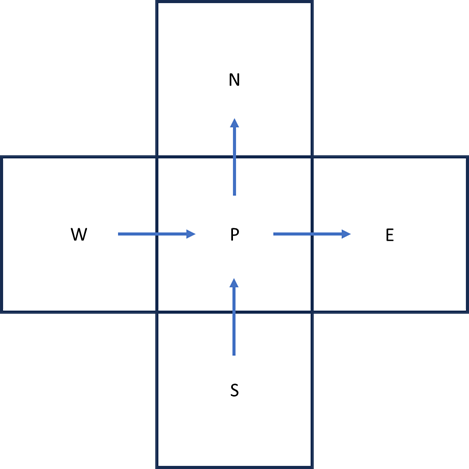
\includegraphics{Figures/FVMgrid.png}
    \caption{Typical 2D Finite Volume Domain}
    \label{fig:FVMgrid}
\end{figure}

Source terms are approximated using linearization, where $\overline{S}=S_c+S_p\phi_p$. The coefficient $a_p=\sum_{N,S,E,W}{a_{nb}+S_p\Delta V}$, where the subscript, $nb$, indicates neighboring points, and $\Delta V$ is the volume of the control volume, P. FVM then introduces under-relaxation to enhance convergence \cite{SIMPLEC}.

Time discretization techniques are often one of two categories: explicit, or implicit. Explicit discretization relies solely on information from the previous time-step, whereas implicit discretization relies on both information from the previous timestep, and information from the next timestep \cite{Anderson1995}.

Another important consideration in CFD simulations is whether to use a segregated or coupled method to solve the governing equations. The main difference between the two methods is that the coupled method combines all of the governing equations into one large linear system of equations, and solves all of the flow variables simultaneously, and employs density-based schemes. On the other hand, segregated solvers are pressure-based and solve flow variables iteratively using several different systems of equations \cite{ransom_1996}.

Stability in a CFD simulation is generally characterized by Von-Neumann Stability Analysis, which essentially says that the round-off error, $\epsilon$, must take the form $|\epsilon^{n+1} / \epsilon^{n}| \leq 1$, where n is the timestep.  Round-off error is represented by an arbitrary function, and that arbitrary function is approximated using a Fourier Series expansion. The result of this analysis leads to a dimensionless number, called the Courant number, shown in Equation \ref{eq:courantNo}, which is a function of the velocity, mesh size, and timestep. The criterion for stability is called the CFL criterion, and generally means that the Courant number must be close to unity for a solution to be stable. It is important to note that this the CFL criteria is generally necessary, but not always sufficient for a stable solution. As solvers get more complex, there are more stability criteria to consider \cite{Anderson1995}.

\begin{equation}
    Co=u\frac{\Delta t}{\Delta x}\ \approx 1
    \label{eq:courantNo}
\end{equation}

\subsection{Flow Discretization Schemes}
\begin{figure}
    \centering
    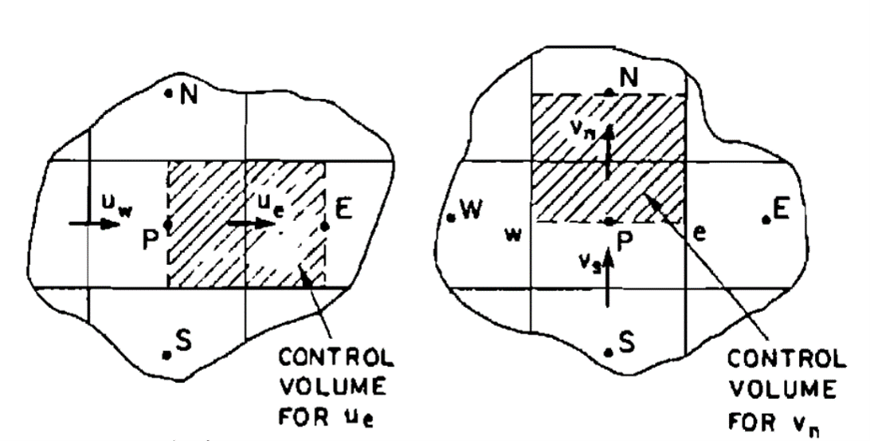
\includegraphics{Figures/faceCenteredCVs.png}
    \caption{Staggered face-centered control volumes}
    \label{fig:faceCenterCVs}
\end{figure}

The flow solver used in this study is a SIMPLEC Algorithm, developed as a modification to the SIMPLE algorithm that allowed for easier implementation and increased computational efficiency \cite{SIMPLEC}. The SIMPLE algorithm takes the general FVM scheme, and staggers the grid shown in Figure \ref{fig:FVMgrid}, to solve for the face-centered control volumes shown in Figure \ref{fig:faceCenterCVs} \cite{Patankar1972ACP}. For the u-component of velocity, the velocity and pressure terms are coupled via Equation \ref{eq:pressureVelocityCoupling},


\begin{equation}
    a_eu_e=\sum_{N,S,E,W}{a_{nb}u_{nb}+b_e+A_e\left(P_p-P_E\right)}
    \label{eq:pressureVelocityCoupling}
\end{equation}

Where e denotes the downwind face from p, A is area, and P is pressure. Here, \\ $a_e=\sum_{N,S,E,W}{a_{nb}+S_e\Delta V}\left(1+\frac{1}{E}\right)$, where $E=\frac{\alpha}{1-\alpha}$, and $\alpha$ is the under-relaxation factor. Pressure and velocity corrections are applied as well, in the form of $P=P^\ast+P^\prime$. These corrections are solved for via 

\begin{equation}
    a_eu_e^\prime=\sum{a_{nb}u_{nb}^\prime}+A_e\left(P_p^\prime-P_E^\prime\right).
    \label{eq:pressureCorrections}
\end{equation} 

With these equations in mind, the procedure can be carried out as follow \cite{Patankar1972ACP}:

\begin{enumerate}
    \item Guess an initial pressure field.
    \item Evaluate coefficients
    \item Evaluate mass source terms (coefficient b)
    \item Solve pressuire corrections at point p
    \item Correct the velocity and pressure fields
    \item Solve for fluxes $\Phi$, and update properties and coefficients
    \item Use the corrected pressure in step 4 as the new guess in step 1
    \item Repeat this process until convergence is reached
\end{enumerate}

One critique of the SIMPLE method is that neglecting the $\sum{a_{nb}u_{nb}^\prime}$ term in Equation \ref{eq:pressureCorrections} is unwarranted because an order of magnitude analysis shows that terms of a similar magnitude are present in the equation \cite{SIMPLEC}. To overcome this limitation, the SIMPLEC method subtracts $\sum{a_{nb}u_{nb}^\prime}$ from both sides of Equation \ref{eq:pressureCorrections}. The new term, $\sum{a_{nb}\left(u_{nb\ }^\prime-u_e^\prime\right)}$, is neglected instead, providing a more consistent approximation \cite{SIMPLEC}. 

\subsection{Multiphase Methods}
\label{sec:multiphase}

The work in this proposal relies heavily on numerical methods for multiphase flow, specifically the Eulerian approach to multiphase flow. In an Eulerian multiphase flow, each phase is modeled as continuous, as opposed to a Lagrangian approach where one or multiple phases are modeled as discrete \cite{GOPALA2008204}. There are several techniques used in Eulerian multiphase flow problems, and they can generally be categorized in one of two ways: surface-tracking, or volume-tracking \cite{GOPALA2008204}. The difference between the two methods can be seen in Figure \ref{fig:SurfaceAndVolumeTracking}.

\begin{figure}
    \centering
    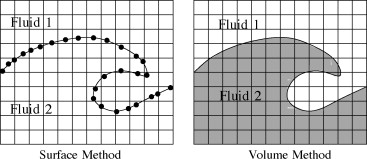
\includegraphics{Figures/surfaceAndVolumeTracking.jpg}
    \caption{Difference Between Surface-tracking (left) and Volume-tracking (right) methods in Eulerian Multiphase Flow \cite{GOPALA2008204}}
    \label{fig:SurfaceAndVolumeTracking}
\end{figure}

The Volume-of-Fluid (VOF) method is a volume method that obtains a single set of flow equations by volume-averaging the governing equations for each fluid. The volume-averaging can best be described in \ref{fig:volumeAveraging} \cite{GOPALA2008204}. Then, the information for each fluid is tracked with a volume fraction transport equation seen in Equation \ref{eq:VOFTransportdiffeq} \cite{HIRT1981201}.

\begin{figure}
    \centering
    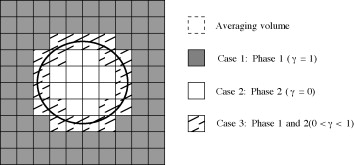
\includegraphics{Figures/volumeAveraging.jpg}
    \caption{Cases for volume averaging in the VOF method \cite{GOPALA2008204}}
    \label{fig:volumeAveraging}
\end{figure}

\begin{equation}
    \frac{\partial\gamma}{\partial t}+\frac{\partial U_i\gamma}{\partial d_i}=0
    \label{eq:VOFTransportdiffeq}
\end{equation}

Issues arise in the VOF method when the above equations are discretized in certain ways. For example, the first order upwind method causes smearing at the interface because of numerical diffusion \cite{GOPALA2008204}.

\subsection{Passive Scalars}
A passive scalar is a useful tool that can be used to track various properties in any given flow field by taking the convection-diffusion equation,

\begin{equation}
    \frac{\partial \phi}{\partial t} + \vec{u} \cdot \nabla \phi=D \nabla^{2} c
    \label{eq:passiveScalarTransport}
\end{equation}

\noindent and coupling it to an arbitrary scalar value, c \cite{Kirby_2010}. From Equation \ref{eq:passiveScalarTransport}, certain parts of the equation can be neglected to produce a different outcome. For instance, if convection should be ignored for the given problem, then $\vec{u} \cdot \nabla c =0$, and only diffusion transport will be modeled. The diffusion coefficient, $D$, can be set arbitrarily to a constant or any field property (such as density or volume fraction) \cite{Kirby_2010, starccm}.

\section{Shock-Droplet Interactions}
\label{sec:shockDropBackground}

\subsection{Shocks and Compressible Flow}

Fluid flow can be broken up into several regimes based on the Mach Number, $Ma$. $Ma$ is the ratio of the velocity of an object to the speed of sound in the surrounding medium, $Ma = u/a$ \cite{GasDynamics}. Generally, the speed of sound can be calculated with

\begin{equation}
    a = \sqrt{\left(\frac{\partial P}{\partial \rho}\right)_{s}},
    \label{eq:sound_speed}
\end{equation}

where P is the pressure, and $\rho$ is the density. The subscript $s$ denotes that the partial derivative is taken isentropically, or at a constant entropy \cite{GasDynamics}. However, if the Ideal Gas assumption is used, the calculation of $a$ is greatly simplified. The local sound speed can be calculated as $a = \sqrt{\gamma R T}$, where $\gamma$ is the ratio of specific heats, $R$ is the specific gas constant, and $T$ is the local temperature. Table \ref{tab:mach_regimes} highlights the different $Ma$ regimes based on their ranges. 

\begin{table}[htp!]
    \centering
    \caption{Mach-number based flow regimes}
    \begin{tabular}{c|c}
       Regime  & Mach Number\\
       \hline
        Incompressible, Subsonic & $Ma < 0.3$ \\
        Compressible, Subsonic &  $Ma < 0.8 $\\
        Compressible, Transonic & $ 0.8 < Ma < 1.2$\\
        Compressible, Supersonic & $1.2 < Ma < 5.0$\\
        Compressible, Hypersonic & $ Ma > 5.0$
    \end{tabular}
    \label{tab:mach_regimes}
\end{table}

The incompressible regime, where $Ma < 0.3$, is the regime in which the density in an infinitesimally small control volume does not change. Hence the flow must be divergence free, meaning that

\begin{equation}
    \nabla \cdot \textbf{u} = 0,
\end{equation}

or equivalently, the material derivative of the density must be zero \cite{johnson2016handbook}.
Beyond the incompressible regime, special care must be taken to handle the fact that density changes with respect to temperature and pressure. An equation of state must be introduced \cite{GasDynamics}, which, in CFD simulations, acts as a nonlinear step in the solver \cite{Anderson1995}. Popular equations of state for gases and liquids will now be summarized.

\subsection{Equations of State}

As mentioned earlier, equations of state (EOS) describe how a material's properties change with respect to other propertioes.

The Ideal Gas Law describes the relationship between a fluid's density, pressure, and temperature \cite{clapeyron1834}. In fluid dynamics, it is often written as

\begin{equation}
    P = \rho R T,
    \label{eq:idealGasLaw}
\end{equation}

This is to say that the pressure of a fluid is directly proportional to its temperature, density, and the specific gas constant. The Ideal Gas Law is valid for gasses at low pressure and high temperatures, and is often used for common gasses such as air, or water vapor. Variations of the Ideal Gas Law exist for other specific circumstances, such as the stiffened EOS, which is useful for describing underwater explosions \cite{stiffenedGas}.

The Real Gas EOS are more complicated than the Ideal Gas Law in the sense that they seek to account for compressibility affects, non-constant specific heats, molecular dissociation, and/or non-equilibrium thermodynamics depending on the use case \cite{vanderwaals, peng-robinson, redlich1949thermodynamics}. These EOS succeed near the critical points of fluids, or at very high pressures. As such, it is sometimes used in hypersonic flows \cite{anderson2019hypersonic}. Many of the Real Gas EOS have empirically-determined parameters. 

A common EOS for liquids is the Tait EOS \cite{tait1888physics}. It relates liquid density to hydrostatic pressure, and is given by

\begin{equation}
    \frac{V_{0} - V}{PV_{0}} = \frac{A}{\Pi + P}.
    \label{eq:tait}
\end{equation}

Here, $P$ is the cumulative pressure (atmospheric plus hydrostatic), $V_{0}$ is the volume at atmospheric pressure, $V$ is the volume at $P$. $A$ and $\Pi$ are empirically-determined coefficients. 

Recently, EOS have been developed to understand how liquids behave when interacting with acoustic waves. One such equation is given by
\begin{equation}
    \rho - \rho_{0} = \left( p_{abs} - P_{0} \right) \left( \frac{1}{c_{0}^{2}} - \frac{\left( \beta - 1 \right) \left( p_{abs} - P_{0} \right) }{\rho_{0} c_{0}^{4}} \right)
    \label{eq:hamiltonEOS}
\end{equation}

which provides second-order compressibility to help capture non-linear distortion in the acoustic wave \cite{hamilton2008nonlinear}. $\beta$ is the coefficient of nonlinearity, ($\approx$ 3.5 for water \cite{Esplin2016}). The low-amplitude speed-of-sound, $c_{0}$, is derived from the nonlinear sound speed,

\begin{equation}
    c = c_{0} + \frac{\left( \beta -1 \right) \left( p_{abs} - P_{0} \right)}{\rho_{0}c_{0}}.
    \label{eq:nonlinearsound}
\end{equation}



\subsection{Cavitation}
Cavitation occurs in water when the water reaches a metastable state in which the static pressure has fallen below the water's vapor pressure \cite{CAUPIN20061000}. At this point, the water must return to equilibrium via nucleation of bubbles \cite{CAUPIN20061000}. Acoustic cavitation is a specific type of cavitation that occurs due to acoustic waves in a droplet, whether they are from shocks \cite{kedrinskii2007shock} or ultrasound \cite{Yasui2018}. The process of cavitation is as follows:

\begin{enumerate}
    \item The static pressure of a region of water falls below vapor pressure
    \item Pre-existing microscopic bubbles of dissolved gas grow in size \cite{Plesset1977} while under tension
    \item Bubbles rapidly collapse due to compression of the surrounding liquid as they reach their maximum radius
    \item A shockwave propagates out from the center of the bubble collapse. In droplets, jutting behavior is observed fas the trailing-edge of the droplet moves inward to fill the void from the bubble \cite{REESE2024104822,Fan2024}.
\end{enumerate}

A diagram of this phenomena is shown in Figure \ref{fig:cavDiagram}

\begin{figure}
    \centering
    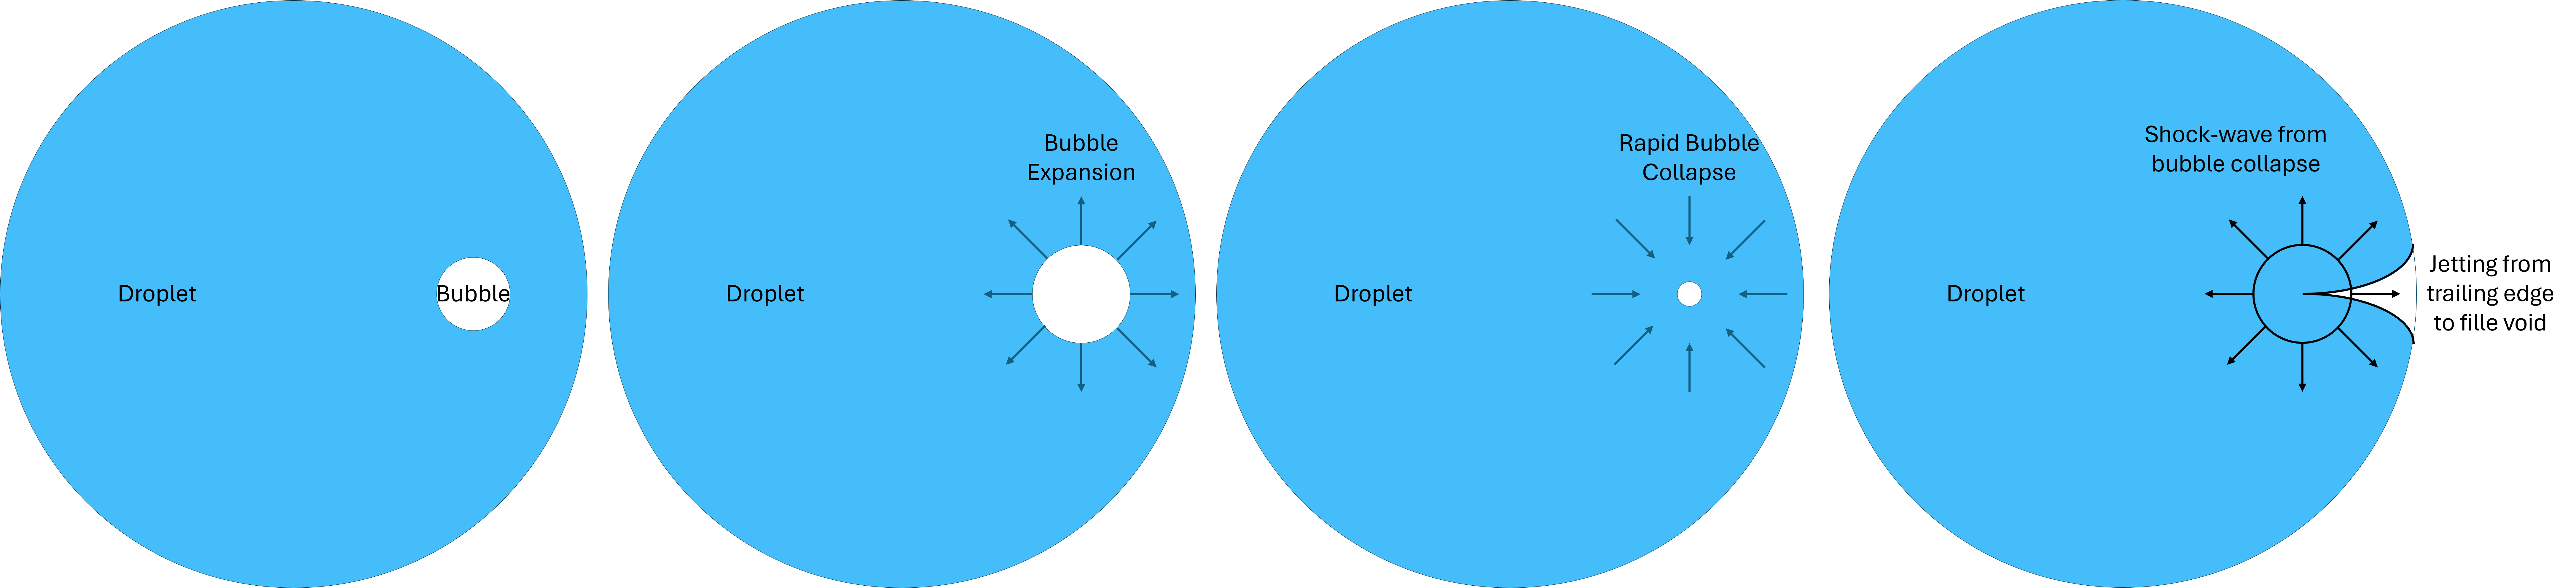
\includegraphics[width=\linewidth]{Figures/cavDiagram.png}
    \caption{Diagram showing the stages of cavitation \cite{Plesset1977, Yasui2018, kedrinskii2007shock}.}
    \label{fig:cavDiagram}
\end{figure}


Since the initial bubbles involved in cavitation are often smaller than the resolution of computational grids \cite{CAUPIN20061000}, a model is needed in order to initialize them in the subgrid scale, and once they achieve a large enough radius, bring them into the grid scale. 

One method of modeling the subgrid bubbles is through a seed-based mass transfer model \cite{Sauer2000InstationrKS}. An important metric for this seed-based approach is the cavitation number,

\begin{equation}
    N_{cav} = \frac{p - p_{sat}}{\frac{1}{2}\rho_{l}U^{2}}.
    \label{eq:cavitationNumber}
\end{equation}

Here, $p$ is the static pressure, $p_{sat}$ is the saturating pressure (or in this case, the vapor pressure of water). $\rho$ is the density, with the subscript $l$ referring to the liquid phase. $U$ is the velocity. This $N_{cav}$ can be thought of as the "potential" for a particular fluid to cavitate. Cavitation requires a surface to occur \cite{CAUPIN20061000}, and impurities in the liquid (such as dissolved gasses) can act as these surfaces \cite{starccm}. In order to use these seeds to propagate cavitation, some assumptions must be made. Primarily, the seeds must initially have the same radius, and they must be spherical and uniformly distributed in the liquid. There is proportionality between the number of seeds in a control volume, and the amount of liquid, such that

\begin{equation}
    N = n_{0}\alpha_{l}V.
    \label{eq:num_seeds}
\end{equation}

Here, $\alpha_{l}$ is the volume fraction of liquid, $n_{0}$ is the seed density, and $V$ is the volume. The total volume of vapor is given by

\begin{equation}
    V_{v} = N V_{b},
    \label{eq:total_vapor_volume}
\end{equation}

and the volume of one particular bubble is just the volume of a sphere. $V_{b} = \frac{4}{3}\pi R^{3}$. Now, it is useful to express the vapor volume fraction in terms of the seed density, radius, and the volume fraction of liquid such that

\begin{equation}
    \alpha_{v} = \frac{V_{v}}{V} = \frac{NV_{b}}{V} = \frac{4}{3}\pi R^{3} n_{0} \alpha_{l}.
    \label{eq:vapor_volume_fraction}
\end{equation}

It is important to be able to calculate $R$ from $\alpha_{v}$ in order to include $R$ in bubble growth calculations further down the line. This can be easily accomplished by rearranging Equation \ref{eq:vapor_volume_fraction} into $R=\left( \frac{3\alpha_{v}}{4\pi n_{0} \alpha_{l}} \right)^{\frac{1}{3}}$. With this, the rate of change of volume of an individual bubble can be calculated as

\begin{equation}
    \frac{dV_{b}}{dt} = 4\pi R^{2} \frac{dR}{dt} = 4\pi R^{2} v_{r}.
    \label{eq:volume_rate_of_change_of_bubble}
\end{equation}

Equation \ref{eq:volume_rate_of_change_of_bubble} introduces the term $v_{r}$, which is the bubble radius growth velocity. This is the primary unknown which cavitation models seek to solve for.

One such model is the Full Rayleigh-Plesset (FRP) equation,

\begin{equation}
    R\frac{dv_{r}}{dt} + \frac{3}{2} v_{r}^{2} = \frac{p_{sat} - p}{\rho_{l}} - \frac{2\sigma}{\rho_{l}R} - 4\frac{\mu_{l}}{\rho_{l}R}v_{r}
    \label{eq:Rayleigh-Plesset}
\end{equation}

which is a nonlinear, ordinary differential equation \cite{rayleigh1917, plesset1949}. The advantage of FRP is that it accounts for the influence of bubble growth acceleration, surface tension, and viscosity. 

The Schnerr-Sauer cavitation model \cite{schnerr2001physical} greatly simplifies FRP by neglecting bubble growth acceleration, surface tension, and viscosity, leading to 

\begin{equation}
    v_{r}^{2} = \frac{2}{3} \left( \frac{p_{sat} - p}{\rho_{l}} \right).
    \label{eq:schnerr-sauer}
\end{equation}

This is a purely algebraic equation that can be readily solved. It has been suggested that in many cases, surface tension and viscous effects can be safely ignored \cite{CavitationBubbleDynamics}. 

\subsection{Droplet Breakup}

When discussing droplets, several critical dimensionless parameters are commonly used: Reynold’s Number (Re), Ohnesorge Number (Oh), and Weber Number (We). The Reynold’s Number has many uses in fluid dynamics, but its primary purpose here is to represent a droplet’s ratio of inertial forces to viscous forces \cite{Cao2020NumericalSO}. The Weber Number represents the ratio of inertial forces to surface tension forces on the droplet \cite{Cao2020NumericalSO}. The Ohnesorge Number and Weber Number are related such that if Oh < 0.1, the viscous forces of the droplet are negligible, and the Weber Number can be used to predict the breakup behavior of the droplet \cite{Cao2020NumericalSO}. Typically in supersonic flow, a droplet experiences catastrophic breakup, meaning that the We is very large (>=500). The inertial forces greatly outweigh the surface tension forces, causing the droplet to be ripped apart violently via the pressure wave. The resulting secondary droplet formation is difficult to predict for these high-Mach situations. This difficulty is potentially due to Rayleigh-Taylor instability-induced piercing, and shear-induced entrainment \cite{Theofanus}. 

The interaction of a rain droplet with a vehicle's bow shock is of great interest. When these two interact, the following occurs \cite{Moylan2010RaindropDI, Forehand2024}:

\begin{enumerate}
    \item As the shock enters the droplet, it causes the liquid to compress
    \item The internal pressure rapidly increases
    \item A pressure wave propagates through the droplet
    \item The pressure starts to exceed the stagnation pressure at the front of the droplet
    \item Once the wave reaches the midpoint of the droplet, the underpressure region switches from tension to compression
\end{enumerate}

These steps are shown visually in Figure \ref{fig:shockDropStages}. These interactions can even cause cavitation, which can influence on the breakup mechanism of the droplet \cite{Briggs2024, Forehand2024}. However, the exact mechanism by which cavitation affects breakup is still unclear.

\begin{figure}
    \centering
    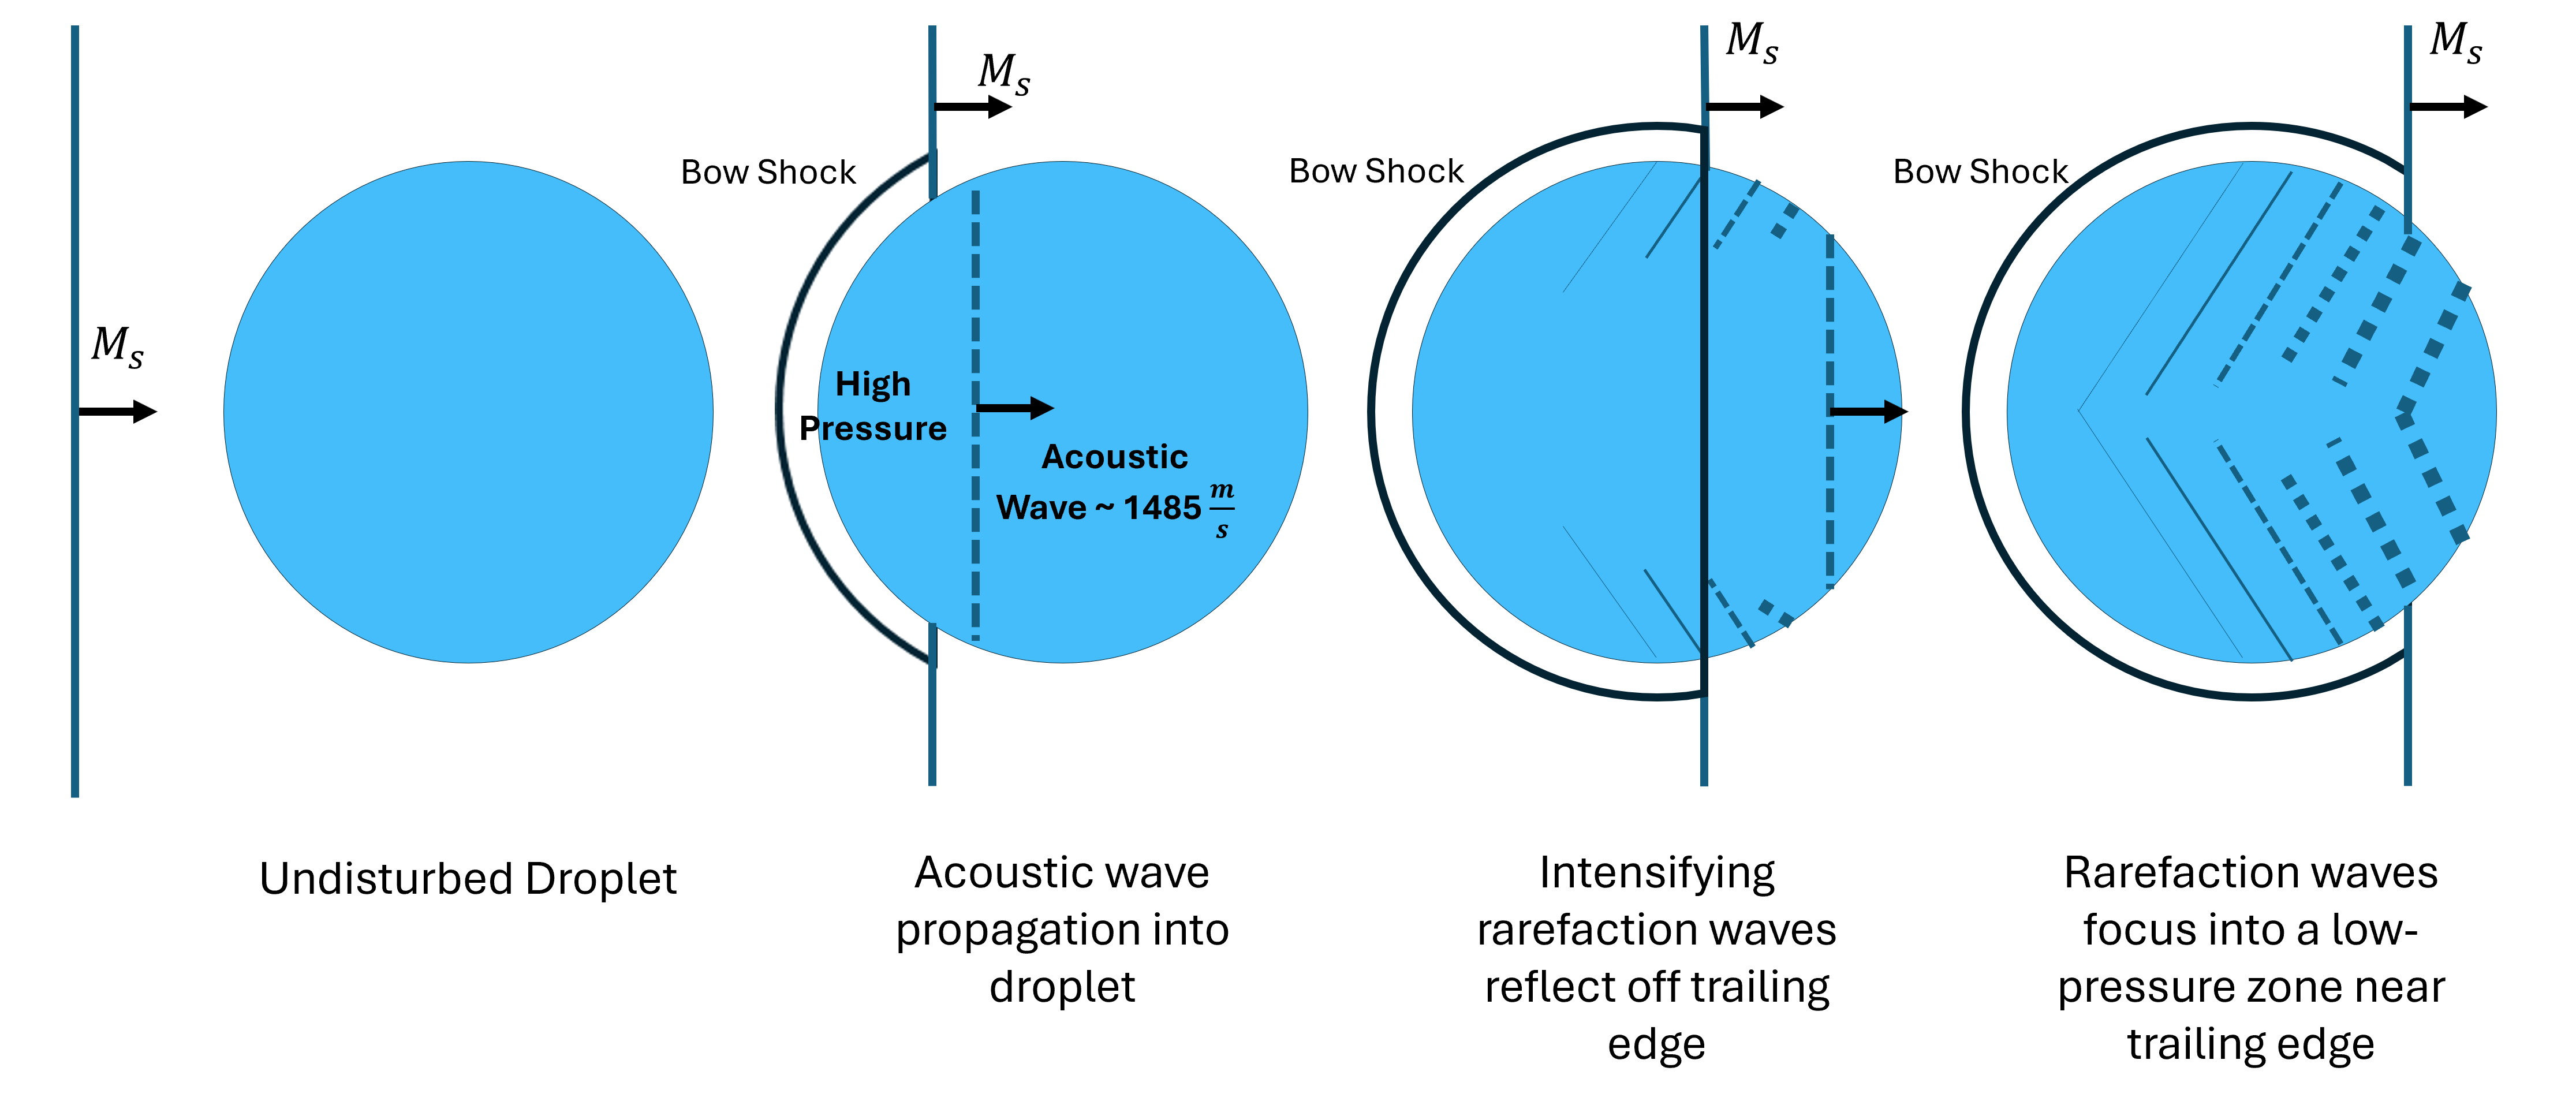
\includegraphics[width=\linewidth]{Figures/stagesOfShockDrop.png}
    \caption{Diagram depicting the various stages of a shock interacting with a droplet before the acoustic wave's first reflection.}
    \label{fig:shockDropStages}
\end{figure}

Numerical studies have been conducted using different droplet breakup models. One such study looked at a detonation wave moving through a water droplet spray \cite{Xu2021EffectOW}, which used the Pilch and Erdman model to predict droplet breakup time. The shear-induced entrainment model also seeks to predict droplet breakup time \cite{Theofanus}. However, all three of these models predict different breakup times and droplet distributions \cite{Bielawski2024}. 

There is some debate over whether cavitation promotes or hinders droplet breakup \cite{Preiss_cav}. Experimental results show that high-intensity cavitation does tend to cause quicker droplet breakup and larger secondary droplets \cite{Preiss_cav, Gall2022, SCHLENDER201584, Freudig2003, Gothsch2011}. However, other work suggests that some cavitation can cause more homogeneous distributions of secondary droplets \cite{LOO1950692}.

For high-Mach flows, experimental results can elucidate information such as cavitation locations \cite{Briggs2024}, but secondary droplet distributions are difficult to quantify because the optical techniques used at the time were not sufficient \cite{nicholls1969}. 
A recent numerical study used Saurel's equations \cite{RICHARDSAUREL20091678} to elucidate properties of the cloud of secondary droplets produced from a primary droplet \cite{Bielawski2024}. Here, the displacement, velocity, and spread of the secondary droplet cloud was calculated, and the atomized droplet distribution was tracked \cite{Bielawski2024}. Focusing on the atomized cloud, however, may take attention away from larger discrete secondary droplets, which can cause more damage to a vehicle.




\section{CMAS/TBC Interactions}
\label{sec:CMAS/TBC_background}

\subsection{Capillary Flow}

Capillary flow occurs when a fluid wicks across a surface without assistance from external forces \cite{kolliopoulos2021capillary}. The phenomena has a wide application spectrum, from lab-on-a-chip devices to study bone porosity \cite{SylvainTaylor} to waste management in microgravity \cite{McCraney}. Early descriptions of capillary flow were proposed by Washburn \cite{Washburn19213} and Lucas \cite{lucas1918ueber}. Here, the capillaries were considered small enough that the regions of turbulent and slip flow would not exist, thus, the flow is dominated by Poiseuille's Law.

Generally, a capillary flow in a cylindrical tube can be described as seen in Figure \ref{fig:capillaryFlowDioagram} and Equation \ref{eq:capillaryFlow}. Here, the pressure that drives the liquid upward is the capillary pressure, $p_{c}$. $p_{c}$ is dependent on the surface tension, $\gamma$, the contact angle of the interface with the wall, $\theta$, and the capillary radius, $r_{c}$. It is also thought of as the difference between the wetting and non-wetting pressure of a pore, which comes from the normal component of the interfacial forces because of surface tension \cite{Chen2022}. $P_{c}$ is also much larger in dynamic capillary flows over static capillary flows \cite{Chen2022}.

\begin{figure}[htp!]
    \centering
    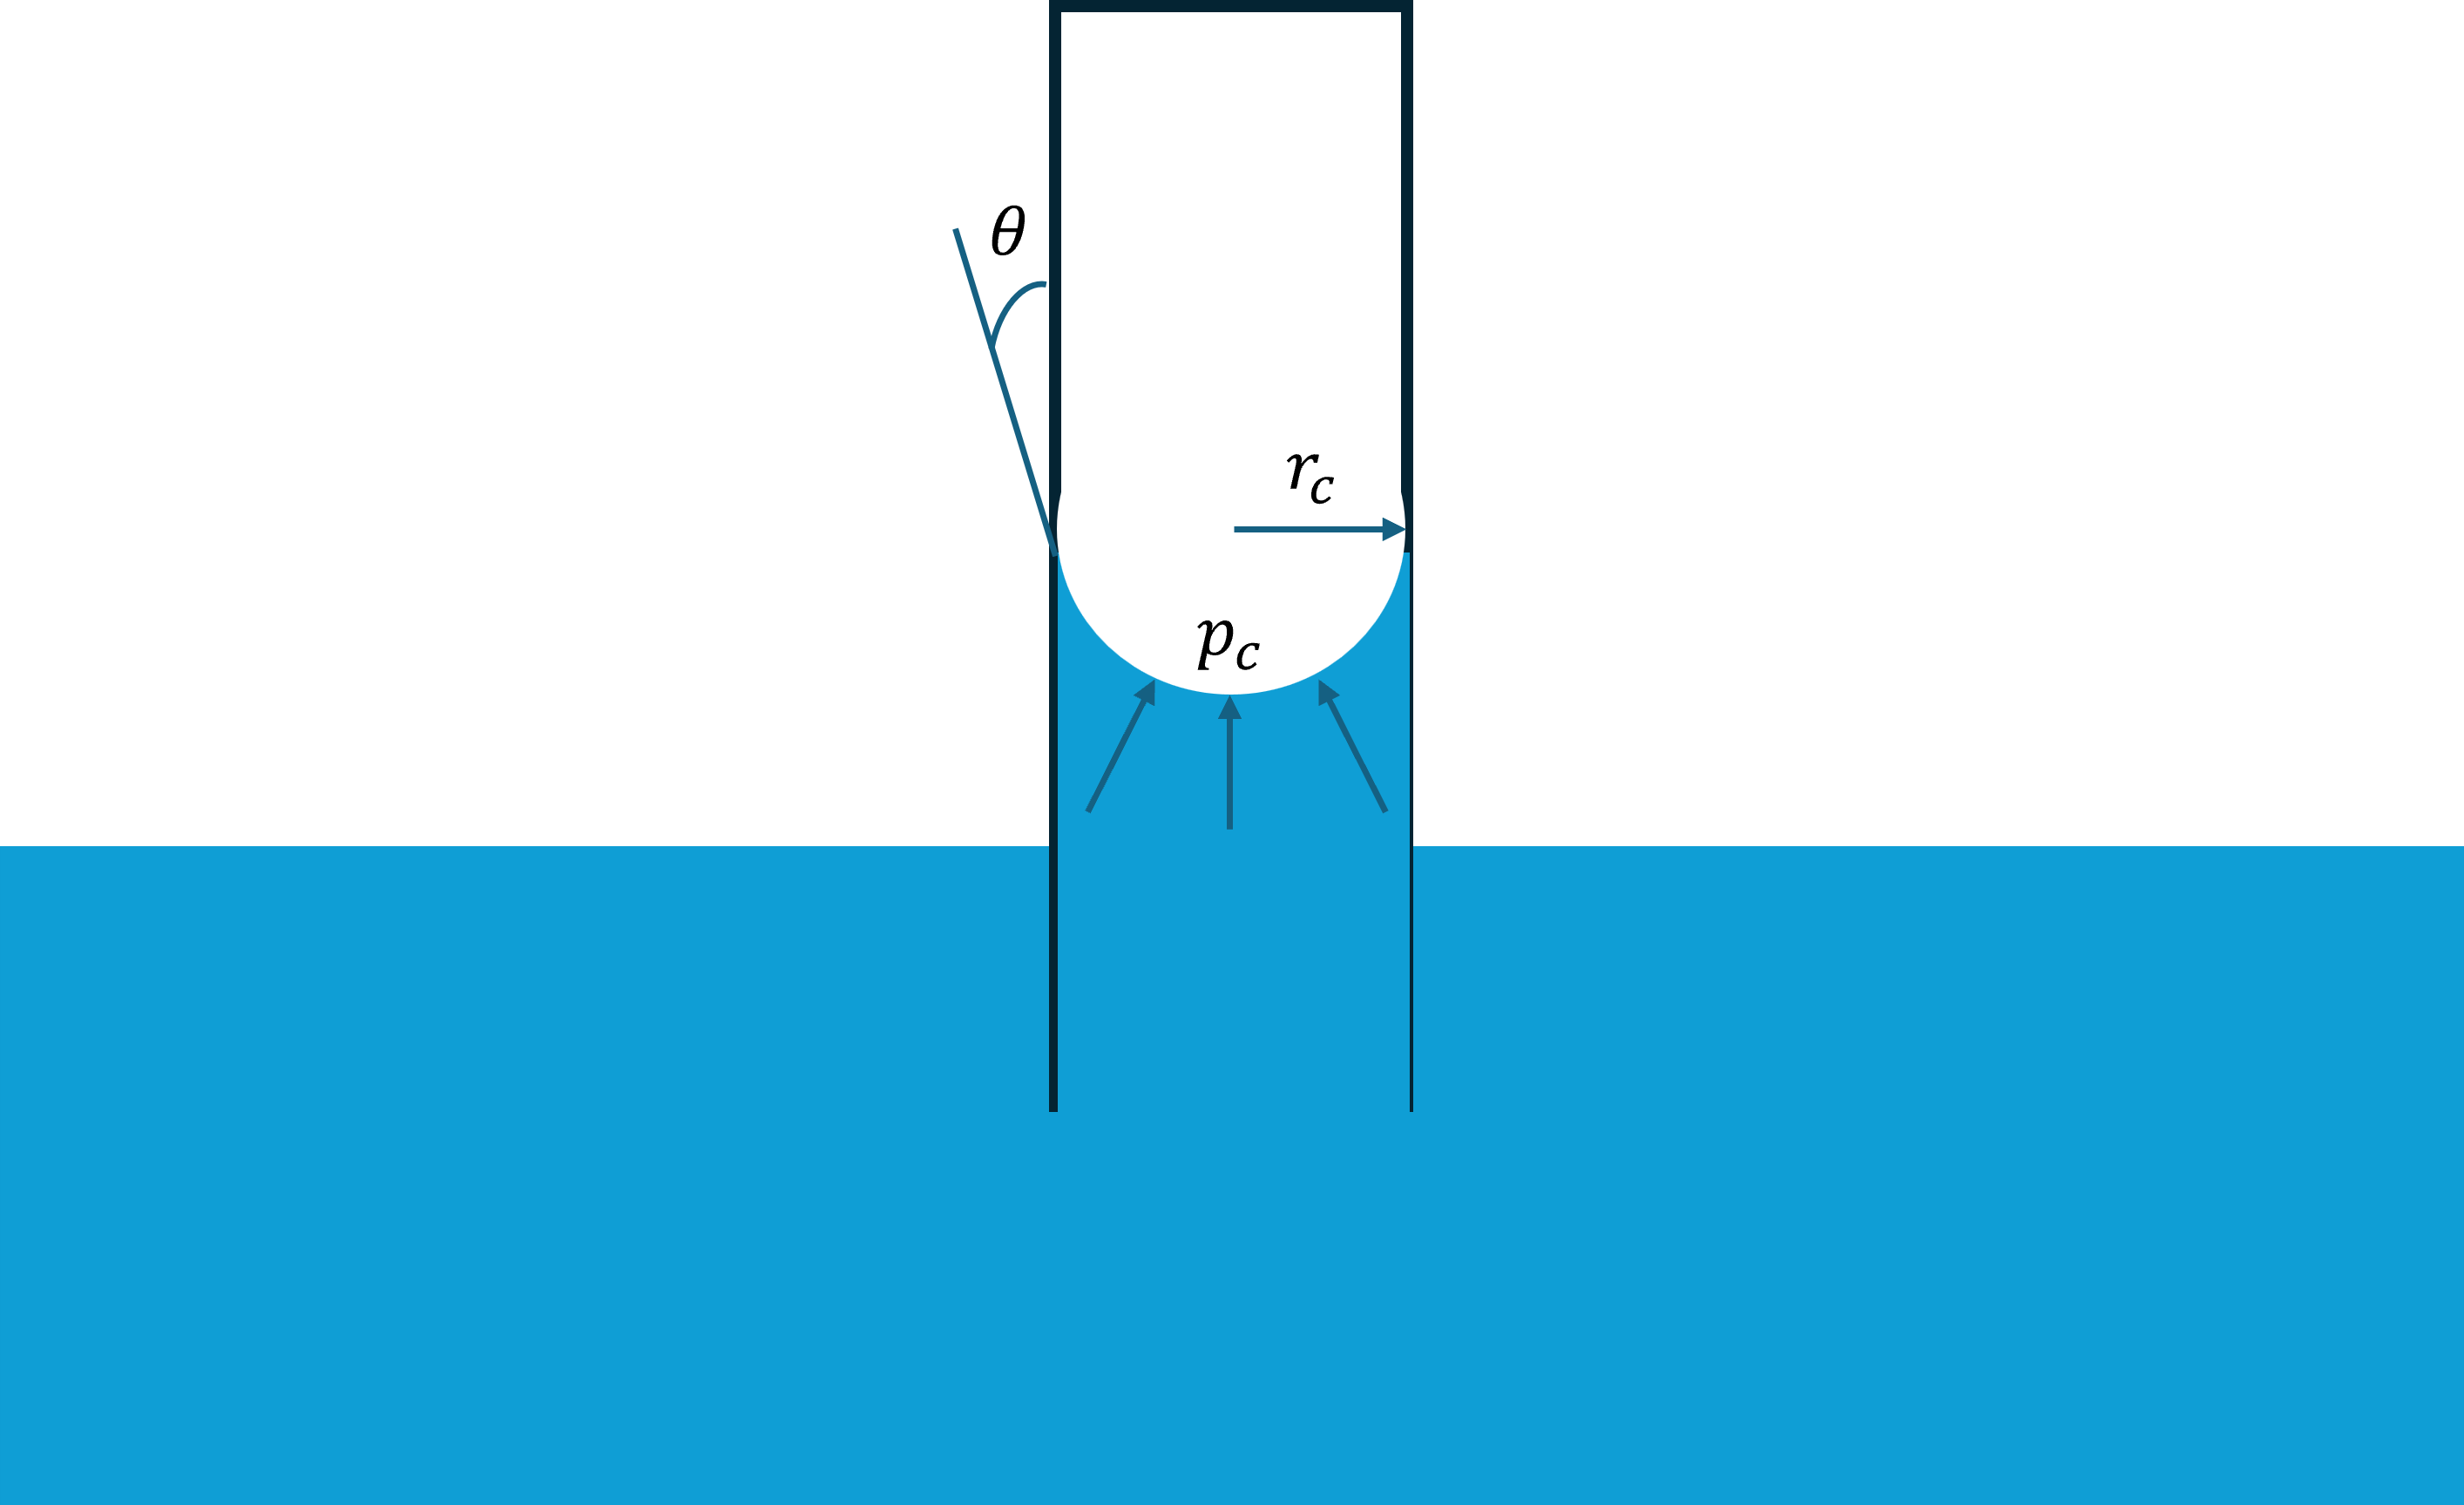
\includegraphics[width=.9\textwidth]{Figures/capillaryFlowDiagram.png}
    \caption{A diagram depicting capillary flow in an air-water system.}
    \label{fig:capillaryFlowDioagram}
\end{figure}

\begin{equation}
    p_{c} = \frac{2\gamma cos\theta}{r_{c}}
    \label{eq:capillaryFlow}
\end{equation}

Washburn and Lucas each describe the position of the curved meniscus as $\hat{z}_{m}$, which has different governing equations depending on the orientation of the tube. In a horizontal tube, the governing equation is $\hat{z}_{m} = \sqrt{\hat{k}\hat{t}}$. Here, $\hat{k}$ is the mobility parameter, which is dependent on the size of the tube, the viscosity, the surface tension, and the contact angle. The flow is dominated by inertial forces at first, but farther down the tube, viscous forces begin to dominate, resulting in different time scales of the flow depending on the current position of the meniscus \cite{kolliopoulos2021capillary}. 
In a vertical cylindrical tube, gravitational effects can become dominant and cause $\hat{z}_{m}$ to reach an asymptotic value \cite{kolliopoulos2021capillary}.

\subsection{Dangers of CMAS Ingestion in Aircraft Engines}
\label{subsec:CMAS_Dangers}
The intake of Calcium-Magnesium-Alumino-Silicate (CMAS) particles by airplane engines poses a threat to the safety and durability of aircraft. For instance, in 1982, all four engines of a Boeing 747 on British Airways Flight 9 failed when the plane flew through a volcanic ash cloud made up of CMAS. When CMAS particles enter the engine, they melt due to the high temperatures and then solidify again on cooling lines \cite{Chen2015}. This can cause damage to compressor blades and thermal barrier coatings, leading to overheating and engine stall \cite{Chen2015}. Helicopters operating in sandy desert environments are at an even higher risk of CMAS damage \cite{Smialek}. The financial impact of CMAS ingestion can also be significant, as demonstrated by the closure of European airspace for six days following the eruption of Eyjafjallajökull in Iceland, which cost commercial airlines an estimated \$1.7 billion \cite{Thehumanconditionblog_2010}. It is crucial to understand how CMAS behaves inside aircraft engines to prevent damage to both airplanes and the global economy. Experimentation and numerical modeling are crucial to understanding CMAS/TBC interactions, and can help regulatory bodies make better safety recommendations. A numerical model of the CMAS infiltration in a TBC has been developed using a Finite-element model in Abaqus \cite{Kabir2019FlowKO}. However, this model approximates surface tension with a suction pressure, and uses constant values for the viscosity of CMAS. Hence, developing a new methodology to simulate the infiltration process could provide a more accurate prediction of infiltration time. 


\subsection{Thermal Barrier Coatings}
Thermal Barrier Coatings (TBCs) are ceramic layers applied to aircraft engine components, such as high-pressure turbine blades, to protect them from prolonged exposure to heat \cite{Bennett2005}. A typical TBC consists of several layers. A metallic substrate is present at the bottom of the coating. This is the material the coating is protecting from heating. Above the metallic substrate is the bond coat; the layer that bonds the metallic substrate to the actual coating. Above that is a thermally-grown oxide layer. Lastly, above the oxide layer is the top coat; the layer responsible for preventing heat transfer. A diagram of a typical TBC is shown in \ref{fig:TBC_diagram} These coatings can reduce component temperatures from 1700 K to around 1200 K \cite{Sirigiri2018}. As higher temperature turbines are required for high thrust applications, it is essential to continue developing and understanding coatings that can more effectively reduce heat transfer in engines. TBC systems can be made using various materials and methods. Electron-beam Physical Vapor Deposition is a manufacturing method in which an anode made out of the desired material is placed inside of a vacuum chamber along with the target object. The anode is bombarded with high-energy electrons, causing the material to undergo a phase change. The now gaseous material precipitates onto everything in the vacuum chamber \cite{EBPVD}. Specifically here, the gaseous 7YSZ is deposited onto a 1mm thick aluminum substrate using a rotation method \cite{Renteria2007}. The microstructure of the TBC can be tuned by changing the rotation speed and temperature of the substrate inside the vacuum chamber \cite{Naraparaju2017}. The columnar microstructure of an EB-PVD coating is shown in Fig. \ref{Fig1}, which shows both ``normal'' and ``feathery'' TBCs, and various stages between. In these cases, the ``normal'' and ``feathery'' microstructures are achieved via the manufacturing parameters in Table \ref{tab:microstructure_manufacture}.

\begin{figure}[htp!]
\centering
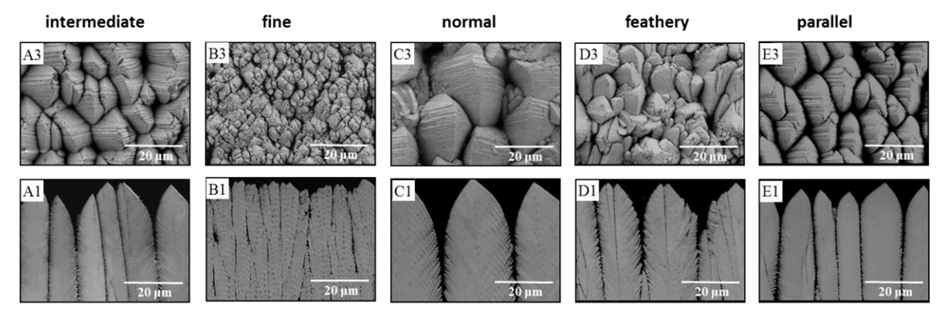
\includegraphics[width=.9\textwidth]{Figures/Fig1.png}
\caption{Various microstructures of EB-PVD TBCs under magnification \cite{Renteria2007}. The top panel depicts the TBC surface, while the lower panel shows a side view from a cut TBC. }
\label{Fig1}
\end{figure}

\begin{figure}[htp!]
\centering
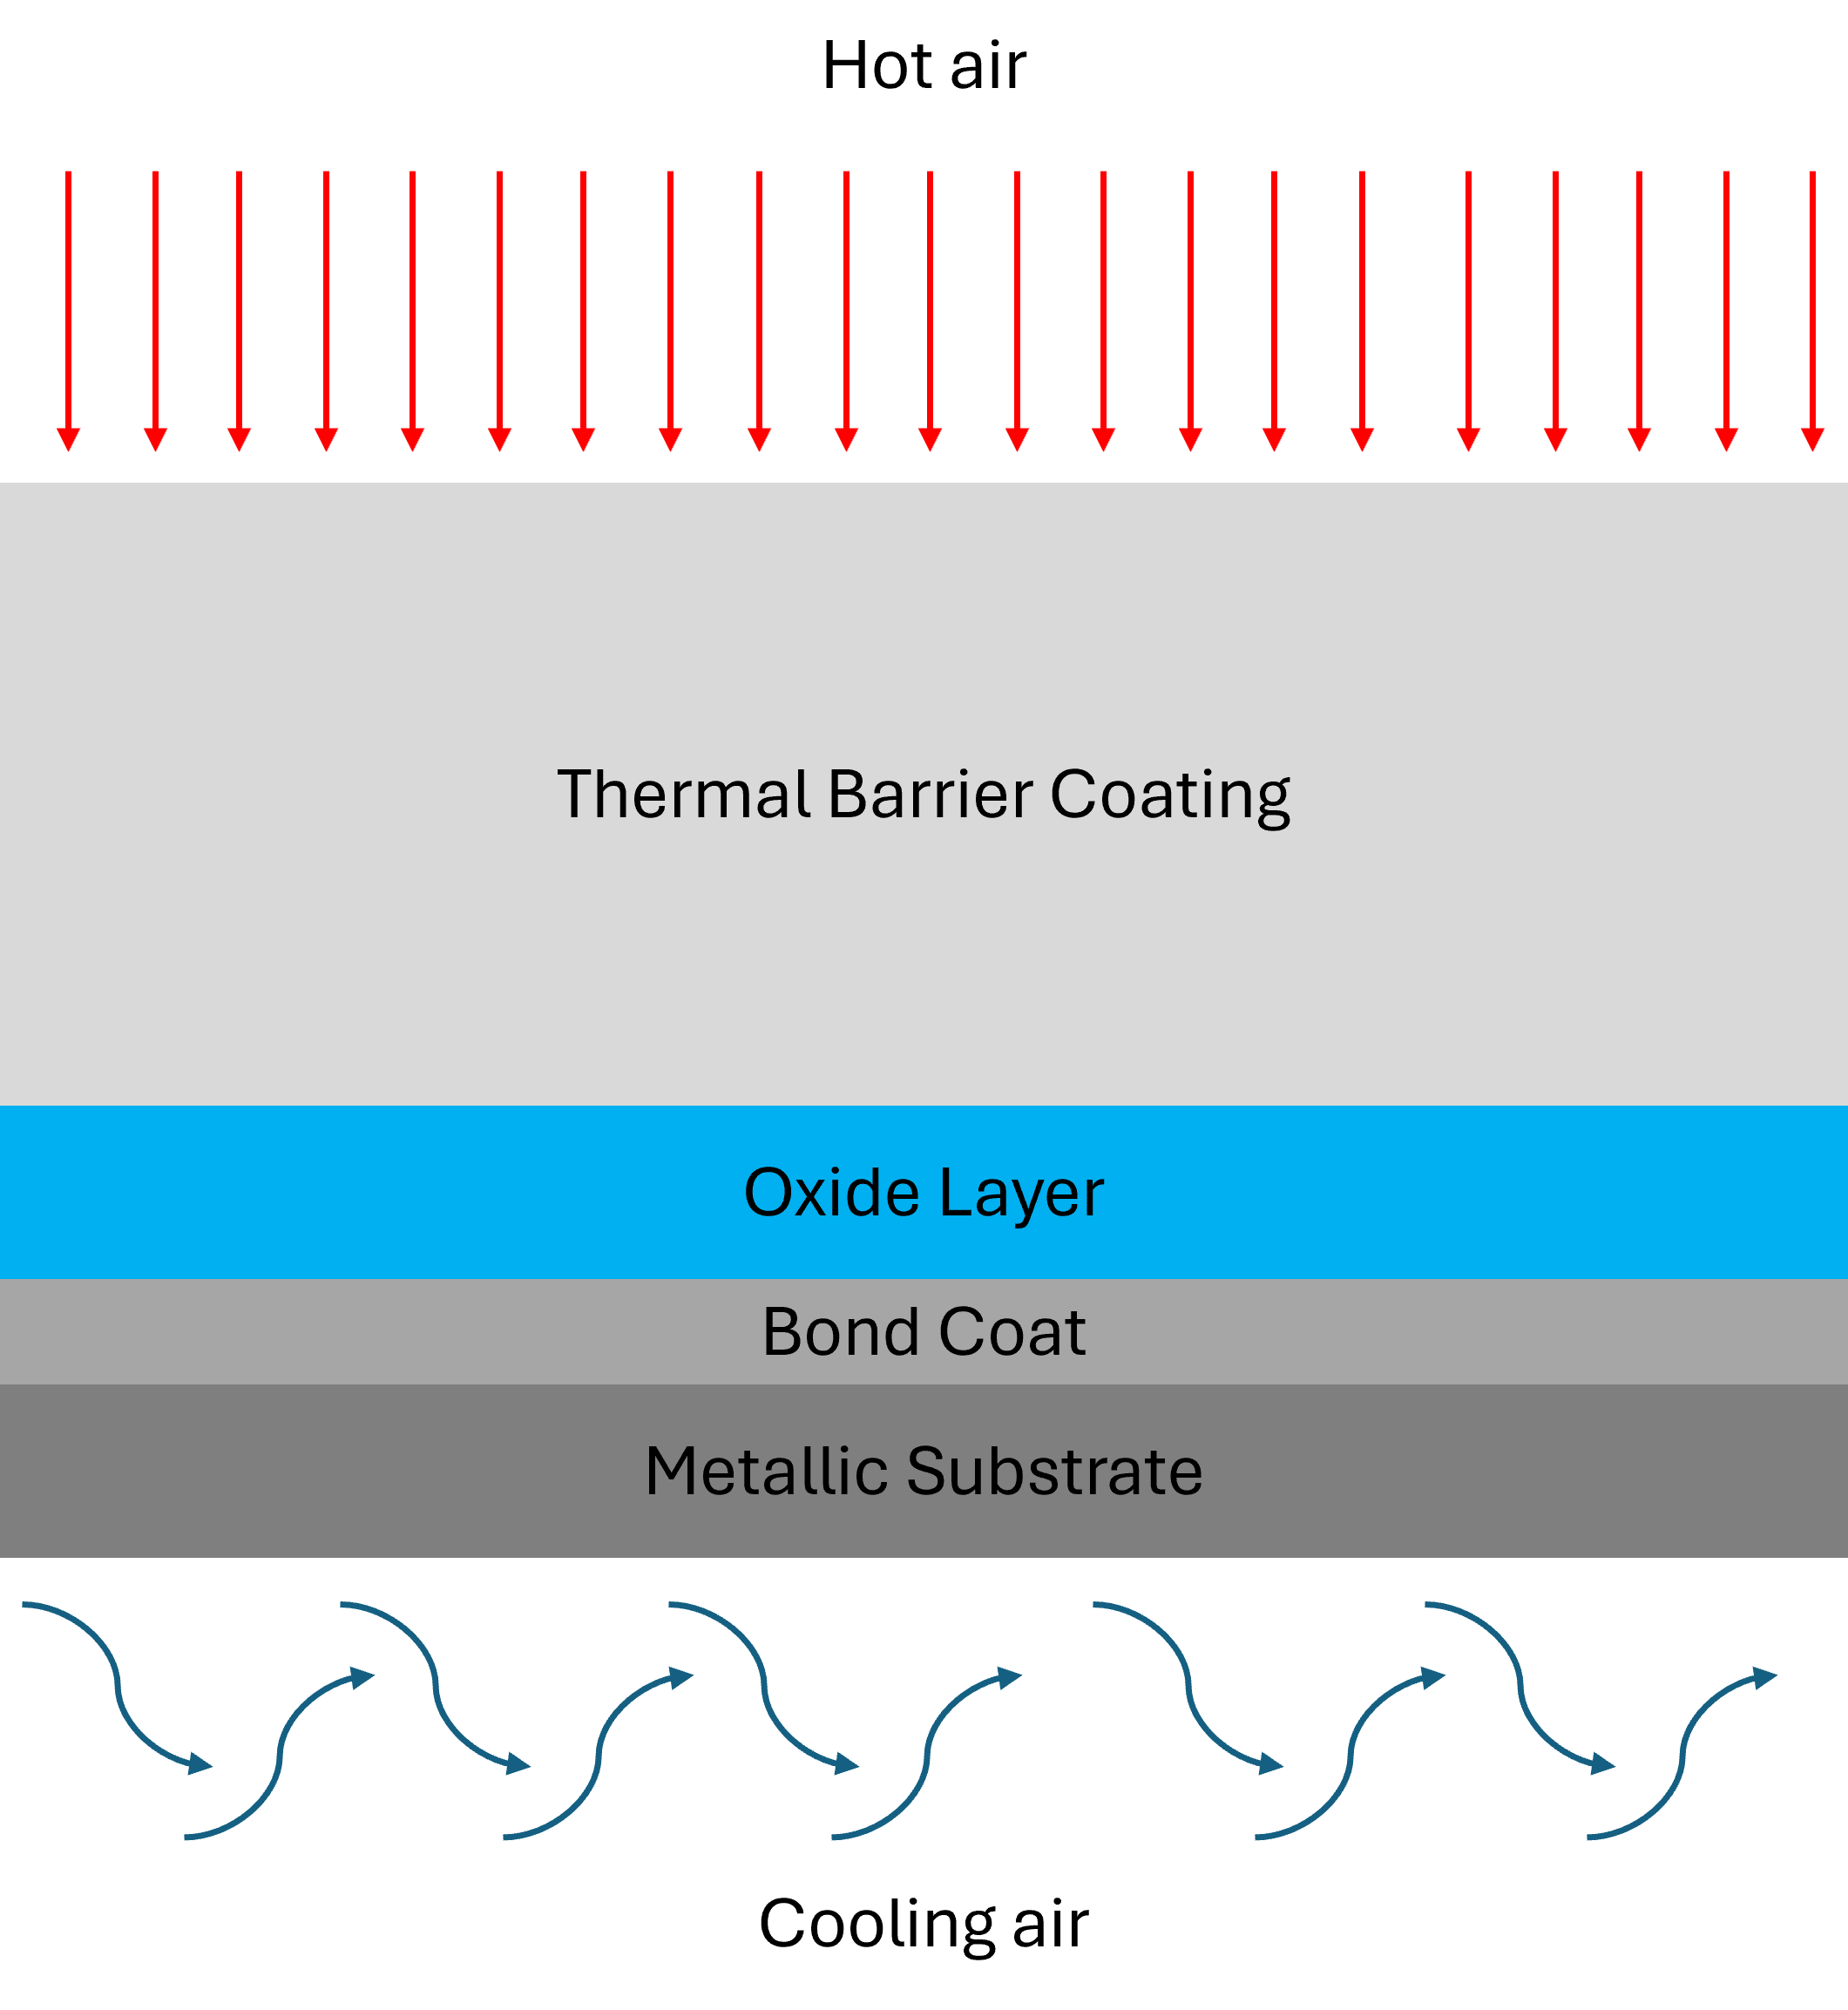
\includegraphics[width=.9\textwidth]{Figures/TBC_diagram.png}
\caption{Diagram showing the layers of the TBC as well as the heating and cooling mechanisms.}
\label{fig:TBC_diagram}
\end{figure}

\begin{table}[htp!]
    \centering
    \caption{TBC microstructure with associated manufacturing parameters}
    \begin{tabular}{c|c|c}
       Microstructure  & Substrate Temperature (\degree C) & Rotation Speed (rpm) \\
       \hline
        Normal & 1000 & 12\\
        Feathery & 840 & 30
    \end{tabular}
    \label{tab:microstructure_manufacture}
\end{table}

\subsection{Damage Mechanisms of CMAS in Aircraft Engines}

A diagram representing a turbofan engine interacting with a debris cloud is depicted in \ref{fig:fan_debris}. CMAS enters an aircraft engine as the aircraft moves through a debris cloud. From this stage, the CMAS particles can impact and erode the airframe, or enter the engine inlet. Once inside the engine, a variety of damaging behavior can occur. The major modes of damage include plugging of cooling channels, melting-solidifcation of particles on nozzle guide vanes (NGV), erosion of compressor blades, and deterioration of high-pressure turbine blade coatings \cite{Chen2015, Naraparaju2019}. Diagrams of these different damage mechanisms are seen in Figures 

\begin{figure}[htp!]
\centering
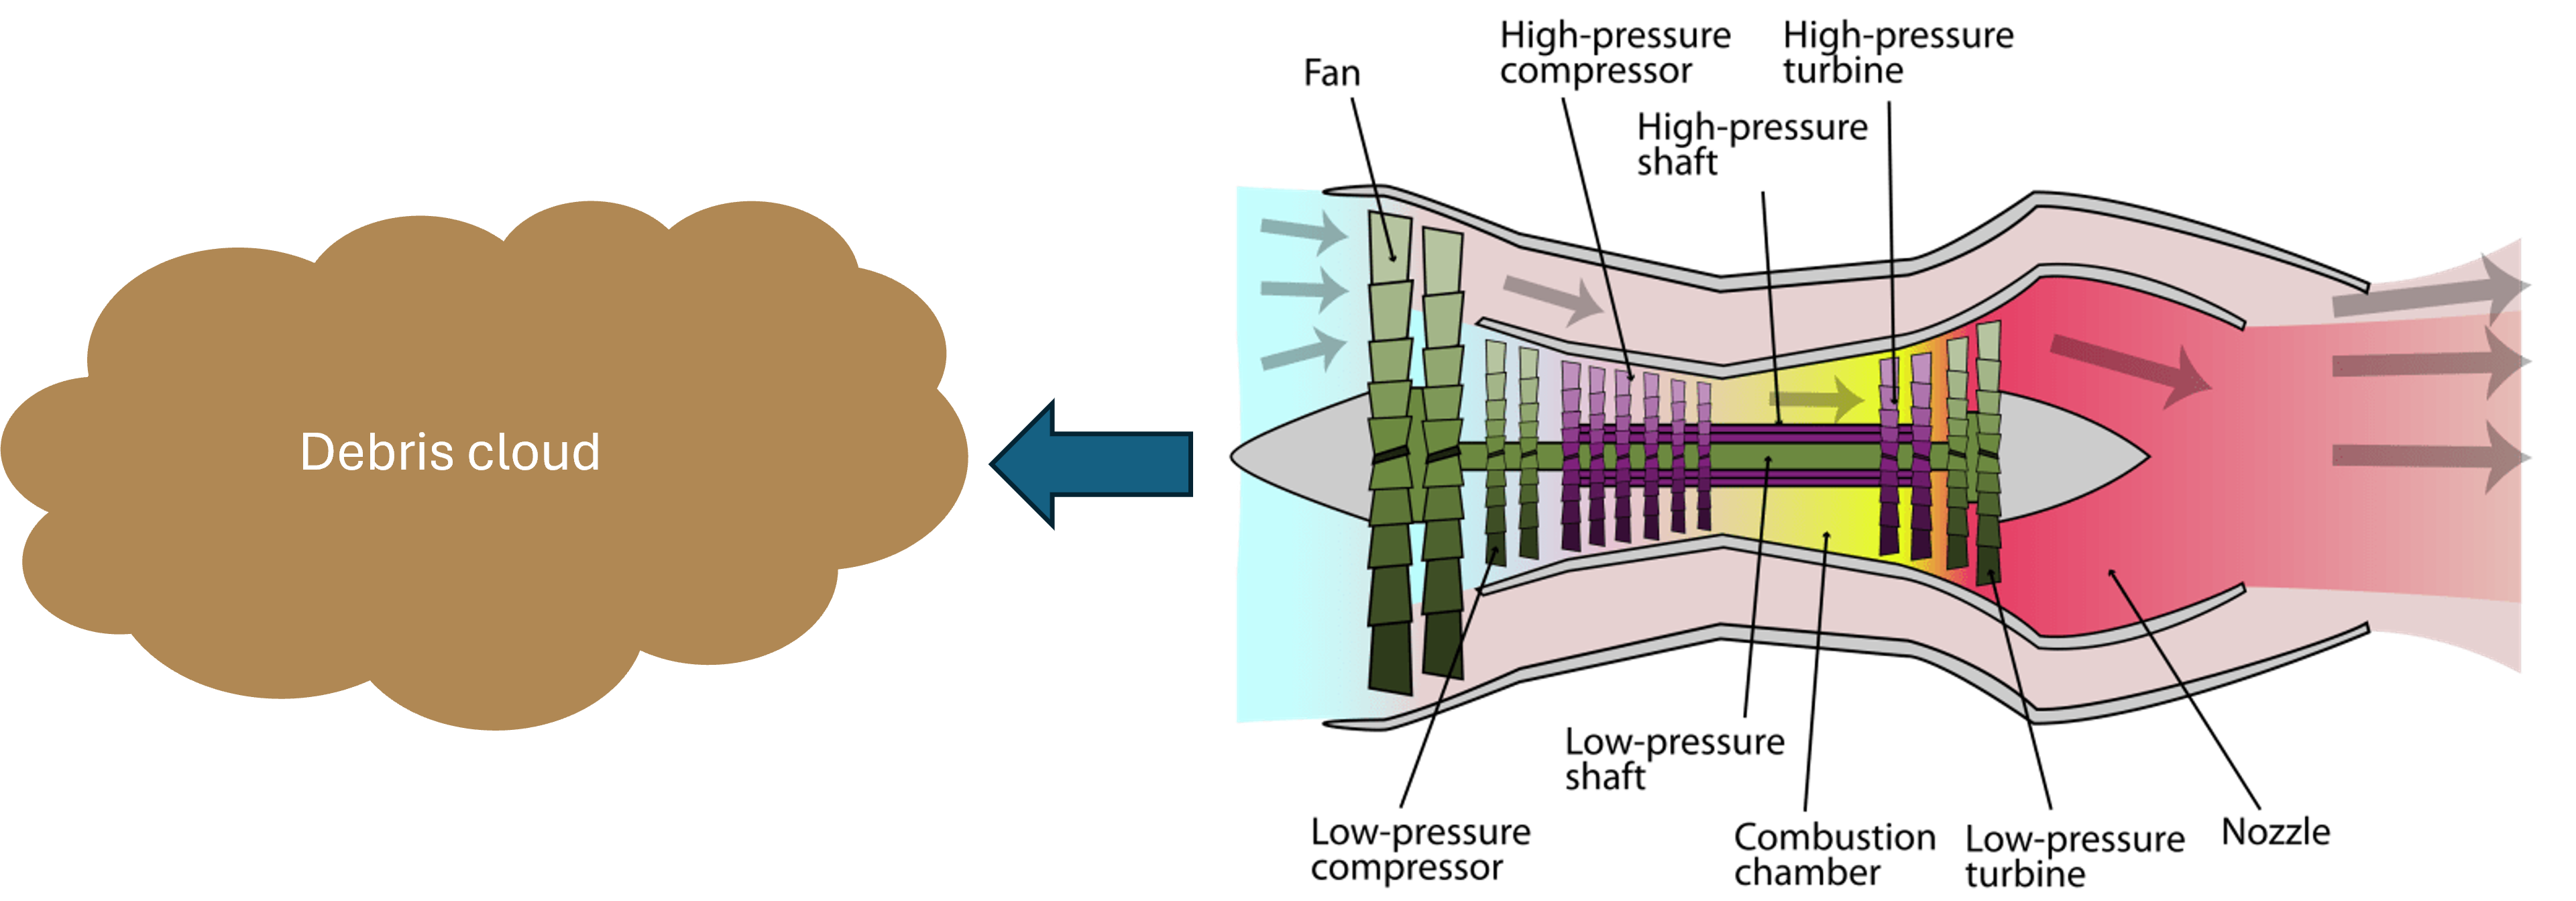
\includegraphics[width=.9\textwidth]{Figures/debrisCloudtoEngine.png}
\caption{A diagram showing a mock-up of a turbofan engine approaching a debris cloud. Components of the engine are labelled \cite{low-bypass_turbofan}.}
\label{fig:fan_debris}
\end{figure}


\begin{figure}[htp!]
\centering
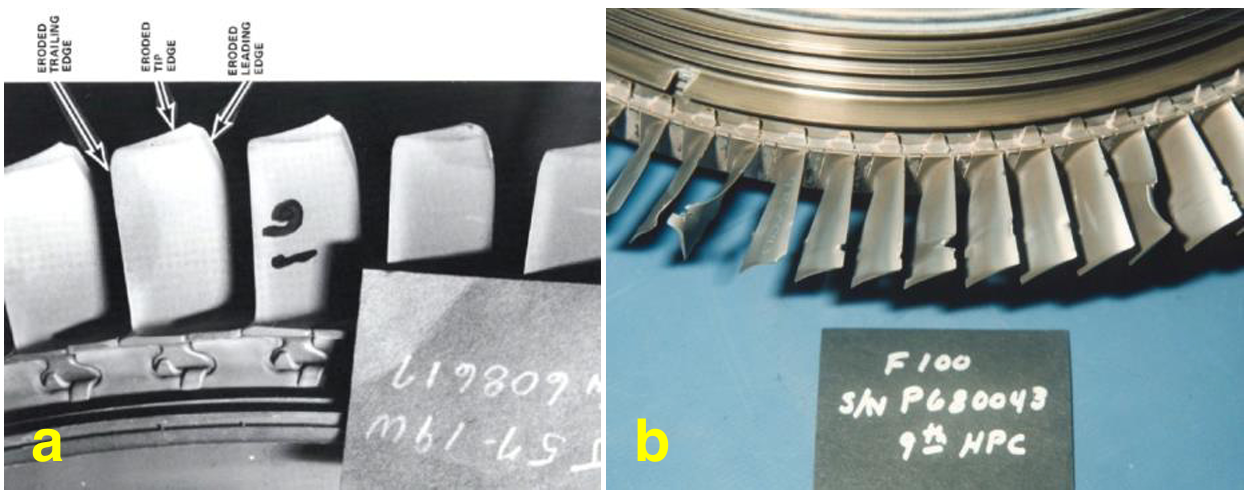
\includegraphics[width=.9\textwidth]{Figures/compressorBladeDamage.png}
\caption{Compressor blade damage after dust exposure in Pratt \& Whittney Engines \cite{Grindle}}
\label{fig:compressorBladeDamage}
\end{figure}

\begin{figure}[htp!]
\centering
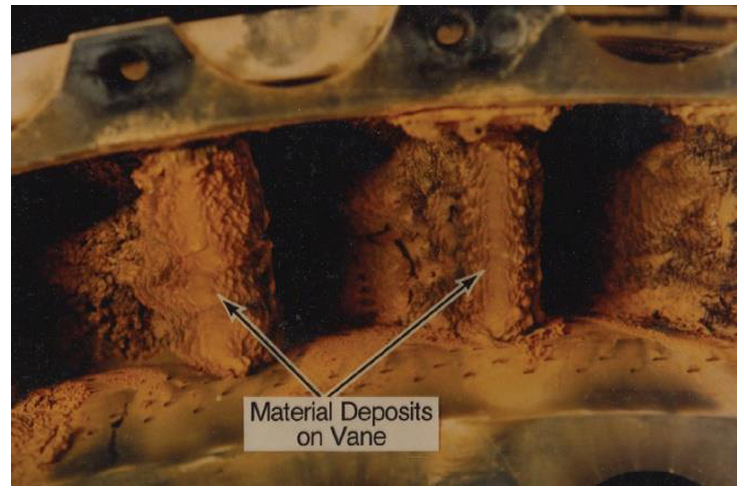
\includegraphics[width=.9\textwidth]{Figures/HPT_damage.png}
\caption{High-pressure Turbine Erosion after dust exposure\cite{Grindle}}
\label{fig:HPT_erosion}
\end{figure}

\subsection{Description of CMAS Infiltration Process}

Due to the established thermal gradient in the TBC, CMAS melts and is able to infiltrate some areas of the TBC, but not others. As a result of this, there is a discrepancy in thermal and mechanical properties within the coating. Strain tolerance decreases, thermal conductivity increases, and the thermal expansion coefficient changes between the infiltrated and uninfiltrated areas \cite{KRAMER200826, WU20111881, KAKUDA2015350}. This discrepancy in properties causes the coating to be susceptible to delamination once the CMAS has infiltrated to a critical depth \cite{MERCER20051029}. The CMAS attack also causes a sintering phenomena to occur, which also erodes TBCs \cite{Peng2012}. As manufacturers seek to help aero-engines achieve higher temperatures for efficiency gains, molten CMAS is becoming more of a problem \cite{Boyce2012}. Depending on composition, most forms of CMAS melt between 1150 - 1250 \degree C \cite{Costa2019,Naraparaju2014,Wellman2010,Kramer2006}. The sintering occurs when the molten CMAS comes into contact with the TBC. In One such case, molten volcanic ash interacted with a YSZ TBC to form yttria iron garnet \cite{Xia2019}.

Current literature has explored several important aspects of CMAS interaction with aircraft engines. One such study includes a computational model exploring CMAS particle fan-blade interaction \cite{Vogel2018}. This study found a distribution of particle sizes that are likely to move past the fan stage in aeroengines \cite{Vogel2018}. Another important study investigated how the impact of CMAS particle size and chemical composition would affect the particle’s time to equilibrate on the nozzle guide vane. The particle’s properties were summarized using the thermal Stokes number. The ratio of particle impact temperature ($T_{p,imp}$) to the temperature of the fluid ($T_f$) was measured. The study showed that the temperature of particles with a $St_{th}$ below unity unity equilibrate with the temperature of the surrounding fluid in a fraction of the surrounding fluid’s response time. $St_{th}$ larger than unity led to particles that take much longer than the surrounding fluid’s response time to equilibrate with the surrounding fluid \cite{Bojdo2019}. This correlation was used as a validation methodology for this method \cite{Cavainolo2022}.

TBC infiltration is widely considered to be a capillary flow problem \cite{Naraparaju2017}, models analgous to pipe flow have been derived for these granular capillary flows. One such model was originally created for water infiltration in soil, and was adapted to the CMAS/TBC infiltration problem \cite{CARMAN1997S32, Chapuis2003616, Naraparaju2019}. Whether these reduced-order models are valid for describing the CMAS/TBC infiltration in a TBC column is not fully understood. The pipe models are intended to describe the bulk flow of fluid through a porous medium \cite{Naraparaju2017}, whereas capillary flow models may better describe the flow in an isolated TBC columnar gap. This brings forth a basic question, \textit{how accurate are the analytical pipe models for isolated TBC columns with complex shapes?}

Previous simulation-based infiltration models have used a FEM approach \cite{Kabir, Sirigiri2018}, but this approach comes with several challenges, including difficulties associated with surface tension forces. Kabir and Sirigiri's approach uses a coupled Euler-Lagrange methodology. Here, the TBC is a rigid-body in a Lagrangian domain, and the molten CMAS is a fluid in an Eulerian domain. However, the Eulerian domain is not multiphase (i.e. the air-CMAS interface is not explicitly resolved). Void cells are used instead of an air-phase, and surface tension forces are modeled at the free-surface. Another drawback of the FEM infiltration model is that it was modeled in an isothermal setting. Hence, the temperature-varying properties of the molten CMAS are not captured. This is important because the viscosity of CMAS is heavily dependent on the temperature \cite{Naraparaju2019}.


\chapter{METHODOLOGY}

\section{Shock-droplet Interactions}
\label{sec:shock-droplet_method}
\subsection{Numerical Methods}
\label{sec:DropletnumericalMethods}
The computational model for this numerical study was developed within Star-CCM+ \cite{starccm}, utilizing the Finite-Volume variation of the Navier-Stokes equations. The SIMPLE-C solver technique was employed \cite{SIMPLEC}, as well as the Volume-of-Fluid (VOF) method \cite{HIRT1981201}. These methods are second-order accurate in space, and first-order accurate in time. The model builds upon research and models developed by Esplin \cite{Esplin2016,esplin2016bulk}, Anderson \cite{Andersom2020}, and Forehand \cite{Forehand2024}. 

The governing equations for the VOF method in Star-CCM+ ver. 18.02.008-R8 \cite{starccm} are shown in a finite-volume formulation and include Conservation of Mass

\begin{equation}
\label{eq:consMass}
    \frac{\partial}{\partial t}\int_{V}\rho dV+\ \oint_{A}{v\bullet d\ A}=\ \int_{V}\left(S\right)dV\ ,\ S=\ \sum_{i}{S_{a_i}\rho_i}
\end{equation}

\noindent Conservation of Momentum

\begin{align}
    \label{eq:consMomentum}
        \frac{\partial}{\partial t}\int_{V}\rho vdV &+ \oint_{A}{\rho v\times v}\bullet\ dA \\
        &= \oint_{A}{\rho I\bullet dA} + \oint_{A}{T\bullet dA} \nonumber \\
        &+ \int_{V}\rho gdV + \int_{V}{f_bdV} \nonumber \\
        &- \sum_{i}\int_{A}{a_i\rho_iv_{d,i}\times v_{d,i}dA} \nonumber
\end{align}

\noindent and Conservation of Energy

\begin{align}
    \label{eq:consEnergy}
        \frac{\partial}{\partial t}\int_{V}\rho EdV &+ \oint_{A}\left[\rho Hv+p+a_i\rho_i{H_iv}_{d,i}\right]\bullet dA \\
        &= -\oint_{A}{{\dot{q}}^{\prime\prime}\bullet dA}+ \oint_{A}{T\bullet v d A} \nonumber\\
        &+ \int_{V}{S_EdV} + \int_{V}{f_bdV} \nonumber
\end{align}

\noindent Equations \ref{eq:consMass}-\ref{eq:consEnergy} couple to the Eulerian Multiphase VOF Transport Equation which is formulated as follows 



\begin{align}
    \label{eq:VOFtrans}
        &\frac{\partial}{\partial t}\int_{V}{a_idV} + \oint_{A}{a_{i}\textbf{v}\bullet d\ A} \\
        &= \int_{V}{\left(S_{a_i}-\frac{a_i}{\rho_{i}}\frac{D\rho_{i}}{Dt} \right) dV} - \int_{V}{\frac{1}{\rho_{i}}\mathrm{\nabla}\bullet}\left(a_i\rho_{i}v_{d,i}\right)dV \nonumber
\end{align}


\noindent In these equations, the subscript i denotes a particular phase (in this case, air, water, or water vapor), $a_{i} = V_{i}/V$ is the volume fraction of a particular phase, and $S_{a_{i}}$ is a source term defined by the initialization of the phases. The VOF method implements a technique called High-Resolution Interface Capturing (HRIC). HRIC imposes a Courant number limit (i.e. Co = 1.0), and if the Courant number is exceeded, then the HRIC scheme reverts back to a standard upwind scheme, which results in a smeared interface. 

The description of the physical model  in this study will encompass the initial and boundary conditions, a description of the domain, and the meshing techniques. More information about the physics (specifically, the initialization of the shock, and cavitation in the droplet) can be found in Forehand's work \cite{Forehand2024}.

\subsubsection{Time Discretization}
\label{sec:metthods_time}

This smeared interface resulting from the VOF method can be corrected by implementing temporal subcycling. The general idea of temporal subcycling is shown in Equation \ref{eq:GeneralTempSubCycle}, where the right-hand side of the equation is a single source term that combines the right-hand side contributions from Equation \ref{eq:VOFtrans}. 

\begin{equation}
\label{eq:GeneralTempSubCycle}
    \alpha^{n+\Delta t}V - \alpha^{n}V + \int_{t^{n}}^{t^{n+\Delta t}}( \ \sum_{A}\alpha_{f}(s) v \cdot da) = \int_{t^{n}}^{t^{n+\Delta t}}(S(\alpha (s),...)ds
\end{equation}

In this work, an implicit multi-stepping version of this temporal subcycling is employed, which gives an unconditionally stable solution, and a sharp interface is achieved if $\frac{CFL}{N_{imp}} \leq 0.5 $. The sub-iterations calculated with Equation \ref{eq:implicitMultiStep1} are summed up to get the overall contribution for the whole time-step.

\begin{equation}
\label{eq:implicitMultiStep1}
    \alpha_{i+1}V - \alpha_{i}V + \tau( \ \sum_{A}\alpha_{f,i+1}(\tau) v \cdot da) = \tau(S(\alpha^{n+\Delta t},...) ~for~ i = 1, 2, ..., N
\end{equation}

A drawback of using the VOF method for the infiltration is the very small time-steps required to resolve the CMAS infiltration. So, adaptive time-stepping combined with sub-iterations was used to balance computational speed and accuracy. A free-surface condition was enforced so that the Courant number ($Co = \frac{u \Delta t}{\Delta x}$) at the interface was around 1.0. Such a criterion is often demanded to limit the interfacial motion to only a cell. The VOF method requires the use of a segregated solver (i.e. the energy equations is solved in a separate system of equations). This solver is second-order accurate in space, and first-order accurate in time. However, the lower-order time accuracy is offset by the implicit multi-stepping in the segregated VOF solver, described in Equations \ref{eq:GeneralTempSubCycle} - \ref{eq:implicitMultiStep1}. 


\subsection{Cavitation Model}
\label{sec:cavitation}
Cavitation models generally involve placing vapor bubble ``seeds'' within a liquid phase. These seeds grow and act as vapor sources The volume source term of the vapor is
\begin{equation}
    Q_{v} = N \frac{dV_{b}}{dt} = 4\pi n_{0}(1- \alpha_{v})VR^{2}v_{r}
    \label{eq:cavVolSource}
\end{equation}

\noindent where $N$ is the number of vapor bubble seeds, $V_{b}$ is the volume of the bubble seed, $n_{0}$ is the number of seeds per unit volume, $\alpha_{v}$ is the vapor volume fraction, $V$ is the total volume of a given control volume, $R$ is the bubble radius, and $V_{r}$ is the bubble radius growth velocity. All of the parameters in Equation~\ref{eq:cavVolSource} are either material properties, or specified by the user. The exception to this is $V_{r}$, which must be modeled as it is unknown. In this CFD study, the bubble growth velocity, $V_{r}$ is determined by the Full Rayleigh-Plesset equation,

\begin{equation}
    R \frac{dv_{r}}{dt} + \frac{3}{2} v_{r}^{2}=\frac{p_{sat} - p}{\rho_{l}}- \frac{2\sigma}{\rho_{l}R} - 4\frac{\mu_{l}}{\rho_{l}R}v_{r}.
    \label{eq:FullRayleighPlesset}
\end{equation}

\subsection{Passive Scalars}
A passive scalar is a useful tool that can be used to track various properties in any given flow field by taking the convection-diffusion equation,

\begin{equation}
    \frac{\partial}{\partial t} \int_{V} \rho \phi_{i}dV + \oint_{A} \rho \phi_{i} \textbf{v} \cdot da = \oint_{A} \textbf{j}_{i}\cdot da +\int_{V} S_{\phi_{i}}dV
    \label{eq:integral_passiveScalarTransport}
\end{equation}

\noindent and coupling it to an arbitrary scalar value, $\phi$ \cite{Kirby_2010}. From Equation \ref{eq:integral_passiveScalarTransport}, certain parts of the equation can be neglected to produce a different outcome. For instance, if convection should be ignored for the given problem, then $\oint \rho \phi_{i} \Vec{v} \cdot da=0$, and only diffusion transport will be calculated. The diffusion coefficient, $\textbf{j}$, can be set arbitrarily to a constant or any field property (such as density or volume fraction) \cite{Kirby_2010, starccm}. 

In this work, passive scalars are used to track several different aspects of the droplet, each passive scalar is discussed below.
\subsubsection{Secondary Droplet Tracking}
\label{sec:secondDropTrack}

The secondary droplets are tracked via 
\begin{equation}
    \frac{\partial}{\partial t} \int_{V} \rho \phi_{i}dV + \oint_{A} \rho \phi_{i} \textbf{v} \cdot da = \int_{V} S_{\phi_{i}}dV
    \label{eq:secondDropPassiveScalar}
\end{equation}
a passive scalar equation. In this passive scalar, diffusion is ignored, and the source term is set such that each droplet cell is seeded with its initial position, that is 
\begin{equation}
    S_{\phi} = \begin{cases}
        X_{i} & t = t_{0}, \frac{D}{D_{droplet}} < 1.0 \\
        0.0 & t \neq t_{0} 
    \end{cases}.
    \label{eq:diffusionSource}
\end{equation}

A similar scalar is set up to track the y-direction as well. This allows a one-to-one mapping of every cell's initial and final position. Information from this scalar can be used to generate distribution data of secondary droplets, even as atomization occurs.



\subsubsection{Accumulation of Forces}
\label{sec:force_accum}
To understand the forces driving physical phenomena in the droplet, two passive scalars are used to track the accumulation of shear and pressure forces.
Firstly, pressure force accumulation was tracked via

\begin{equation}
    \frac{\partial}{\partial t} \int_{V} \rho \phi_{i}dV = \int_{V} S_{\phi_{P}}dV,
    \label{eq:pressureScalar}
\end{equation}

\noindent where 
\begin{equation}
    S_{\phi_{P}} = \Delta P \times \alpha_{H_{2}O}\times V_{cell}^{1/3}.
    \label{eq:pressureSource}
\end{equation}

\noindent Here, $\Delta P = \partial P / \partial x$, so the pressure gradient is tracked, and scaled by the cell length in the x-direction to reconstitute pressure force. Equations~\ref{eq:pressureScalar} and~\ref{eq:pressureSource} are defined such that, when Equation~\ref{eq:pressureScalar} is integrated through time in a given cell, 

\begin{equation}
    \phi_{P} =  \int_{0}^{t_{f}} \left( \alpha_{H_{2}O}(t) \times \Delta P(t) \times V_{cell}^{1/3} \right) dt. 
    \label{eq:pressureIntegrated}
\end{equation}

\noindent This same method is carried out for the shear stress as well, where

\begin{equation}
    \phi_{\tau} =  \int_{0}^{t_{f}} \left( \alpha_{H_{2}O}(t) \times \tau(t) \right) dt. 
    \label{eq:shearIntegrated}
\end{equation}

\noindent Here, the shear stress does not need to be scaled since the gradient is not being calculated. Now we have two passive scalars whose values represent the accumulation of the two fundamental forces driving droplet deformation and breakup.

\subsection{One-way Coupled Cavitation and CFD Model}
\label{sec:onewaycav}
In this section, we propose a novel method of coupling CFD data and a cavitation model. Here, data from a CFD simulation without a cavitation model is extracted. Then, the CFD data is used as input for an analytical cavitation model. The cavitation model proposed by Esplin \cite{esplin2016bulk, Esplin2016} predicts the bubble radius based on the bubble expansion velocity and the time the bubble is under tension via,

\begin{equation}
    R \left( t_{2} \right) \approx \dot{R}_{max}T \approx \sqrt{\frac{2 \left( p_{vap} - \Bar{p} \right)}{3 \rho_{0}}}T
    \label{eq:bubbleRad}
\end{equation}

\noindent Here, $T=t_{2}-t_{1}$, where $t_{1}$ is the time when $p_{abs}$ becomes less than $p_{vap}$ and $t_{2}$ is the time when $p_{abs}$ rises above $p_{vap}$ once again. A time-averaged pressure, $\Bar{p}$, is calculated during $T$. The variables on the RHS of Equation \ref{eq:bubbleRad} are calculated in the CFD simulation. From here, $R \left( t_{2} \right)$ is calculated and used as input for the rest of Esplin's cavitation model. That is, cavitation criteria and cavitation threshold \cite{esplin2016bulk,Esplin2016} is calculated analytically following the CFD calculation. Integrating the CFD equations with a cavitation model, like Full Rayleigh-Plesset, can frequently result in numerical instabilities.  By isolating the cavitation model from the CFD solution, we can enhance stability since it prevents the cavitation model from influencing the CFD’s stability. Nonetheless, this approach also means that the cavitation model’s impact on the CFD solution is not captured.

\subsubsection{Calculating Cavitation Time and Time-averaged Underpressure}
\label{subsec:cav_time_and_underpressure}
As discussed above, $T$ and $\Bar{p}$ must be calculated within the CFD solution. This can be accomplished with two additional passive scalars, 

\begin{equation}
    \phi_{T} = \begin{cases}
        \int dt & p_{abs} < p_{vap}\\
        0 & p_{abs} \geq p_{vap}
    \end{cases}
    \label{eq:cavTimeScalar}
\end{equation}

\noindent and 

\begin{equation}
    \phi_{\Bar{p}} = \begin{cases}
        \int p_{abs} dt & p_{abs} < p_{vap}\\
        0 & p_{abs} \geq p_{vap}
    \end{cases}
    \label{eq:pbarscalar}
\end{equation}

\noindent where $\Bar{p} = \phi_{\Bar{p}}/T$.  However, the shock reflects multiple times within the droplet, resulting in multiple periods of bubble growth. Hence, the calculation must be carried out for $T_{1, 2,...,n}$ where n is the number of reflections that cause significant pressure drops.


\subsection{Droplet Shape}
\label{sec:dropShapeMethod}

Here, a method is introduced to track the ellipticity, or "flattening" of a droplet ($f_{d}$). $f_{d}$ is calculated via
\begin{equation}
    f_{d} = \frac{a-b}{a},
    \label{eq:flattening}
\end{equation}
\noindent where a is the major diameter of the ellipsoid, and b is the minor diameter of the ellipsoid. One key assumption, given the axisymmetric nature of the domain, is that the dimensions a and c in Figure~\ref{fig:ellipsoid} are always the same length. In a three-dimensional model, this would not necessarily be the case.

\begin{figure}
    \centering
    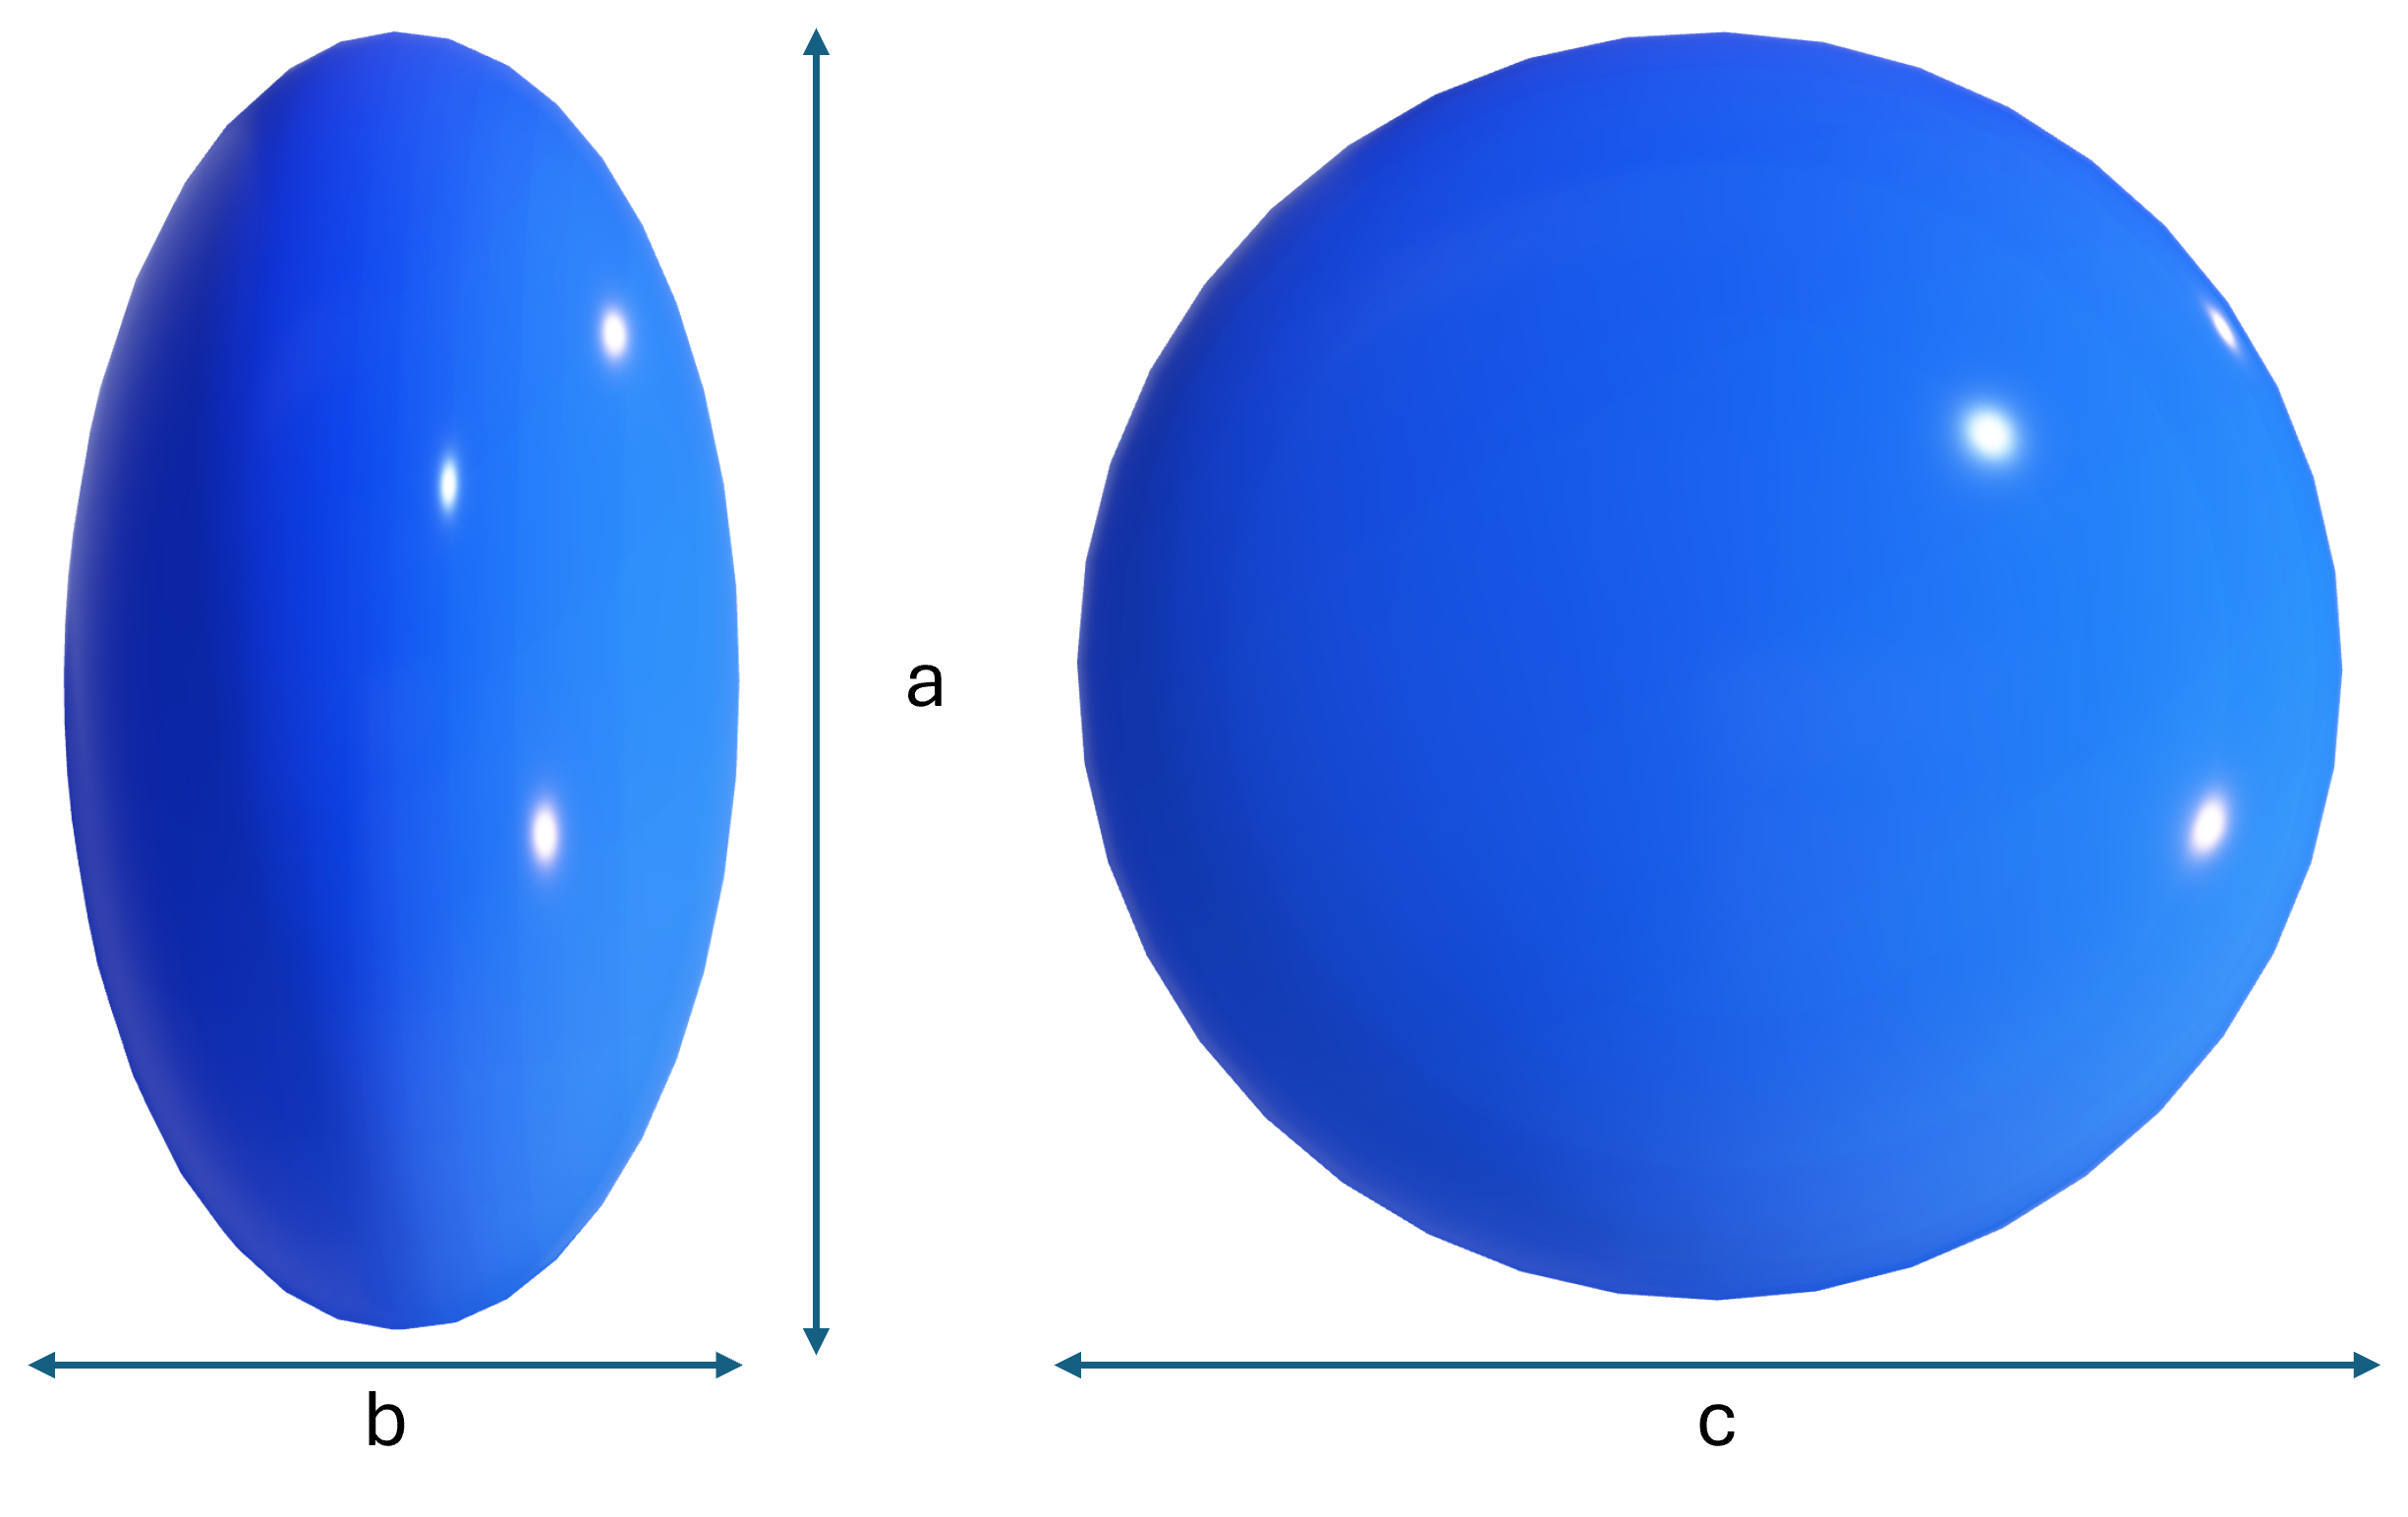
\includegraphics[width=0.8\linewidth]{Figures/ellipsoid.png}
    \caption{Diagram of an ellipsoid representing a deformed droplet, where the diameters a,b, and c are labeled. This figure demonstrates the congruency of diameter a and diameter c}
    \label{fig:ellipsoid}
\end{figure}

A challenge arises when trying to pick where to measure the diameters $a$ and $b$. 
Since the droplet does not deform into a perfect ellipse, a methodology is devised to geometrically normalize the deformed droplets to that of an ellipse.
The method involves calculating the moments of inertia ($I_{xx}$ and $I_{yy}$)  of the droplet over time. 
To do this, the center of mass of the droplet was found, and $I_{xx}$ and $I_{yy}$ of each cell was calculated about that center of mass.
Then, $I_{xx}$ and $I_{yy}$ of each cell was added up to get the total $I_{xx}$ and $I_{yy}$ of the droplet, such that

\begin{equation}
    I_{xx} = \sum_{i=1}^{N} \Delta y_{i}^{2} m_{i},
    \label{eq:MOI_x}
\end{equation}

\noindent and 

\begin{equation}
    I_{yy} = \sum_{i=1}^{N} \Delta x_{i}^{2} m_{i}.
    \label{eq:MOI_y}
\end{equation}

Here, $i$ indicates a particular cell, $N$ represents the total number of cells in the droplet, $\Delta y_{i}$ is the distance from the cell center to the droplet's center of mass, $m_{i}$ is the cell's mass
Next, the Equations \ref{eq:MOI_x} and \ref{eq:MOI_y} are set equal to $\frac{\pi}{4} b^{3} a$ and $\frac{\pi}{4} b a^{3}$ respectively.
These are the equations that define the MOI of an equivalent ellipse. 
From here, $a$ and $b$ can be calculated from that equivalent ellipse.

% A parameter, called the non-sphere, is introduced to relate the droplet's deformed shape to its initial spherical shape. The non-sphere parameter is calculated as in Equation \ref{eq:non-sphere}

% \begin{equation}
%     non-sphere = \iiint_V \begin{cases}
%         \begin{cases}
%             \alpha dV & \alpha < 1 \\
%             0 & \alpha = 1
%         \end{cases} & r < R \\
%         \alpha dV & r \geq R
%     \end{cases}
%     \label{eq:non-sphere}
% \end{equation}

% \noindent Here, the volume-integral of the $\alpha_{H2O}$ is taken to find the amount of liquid that is outside the initial radius of the droplet. A term accounting for partially liquid cells inside the radius is added as well. A diagram of what this is intended to track is shown in \ref{fig:non-sphereDiagram}. 
% \begin{figure}
%     \centering
%     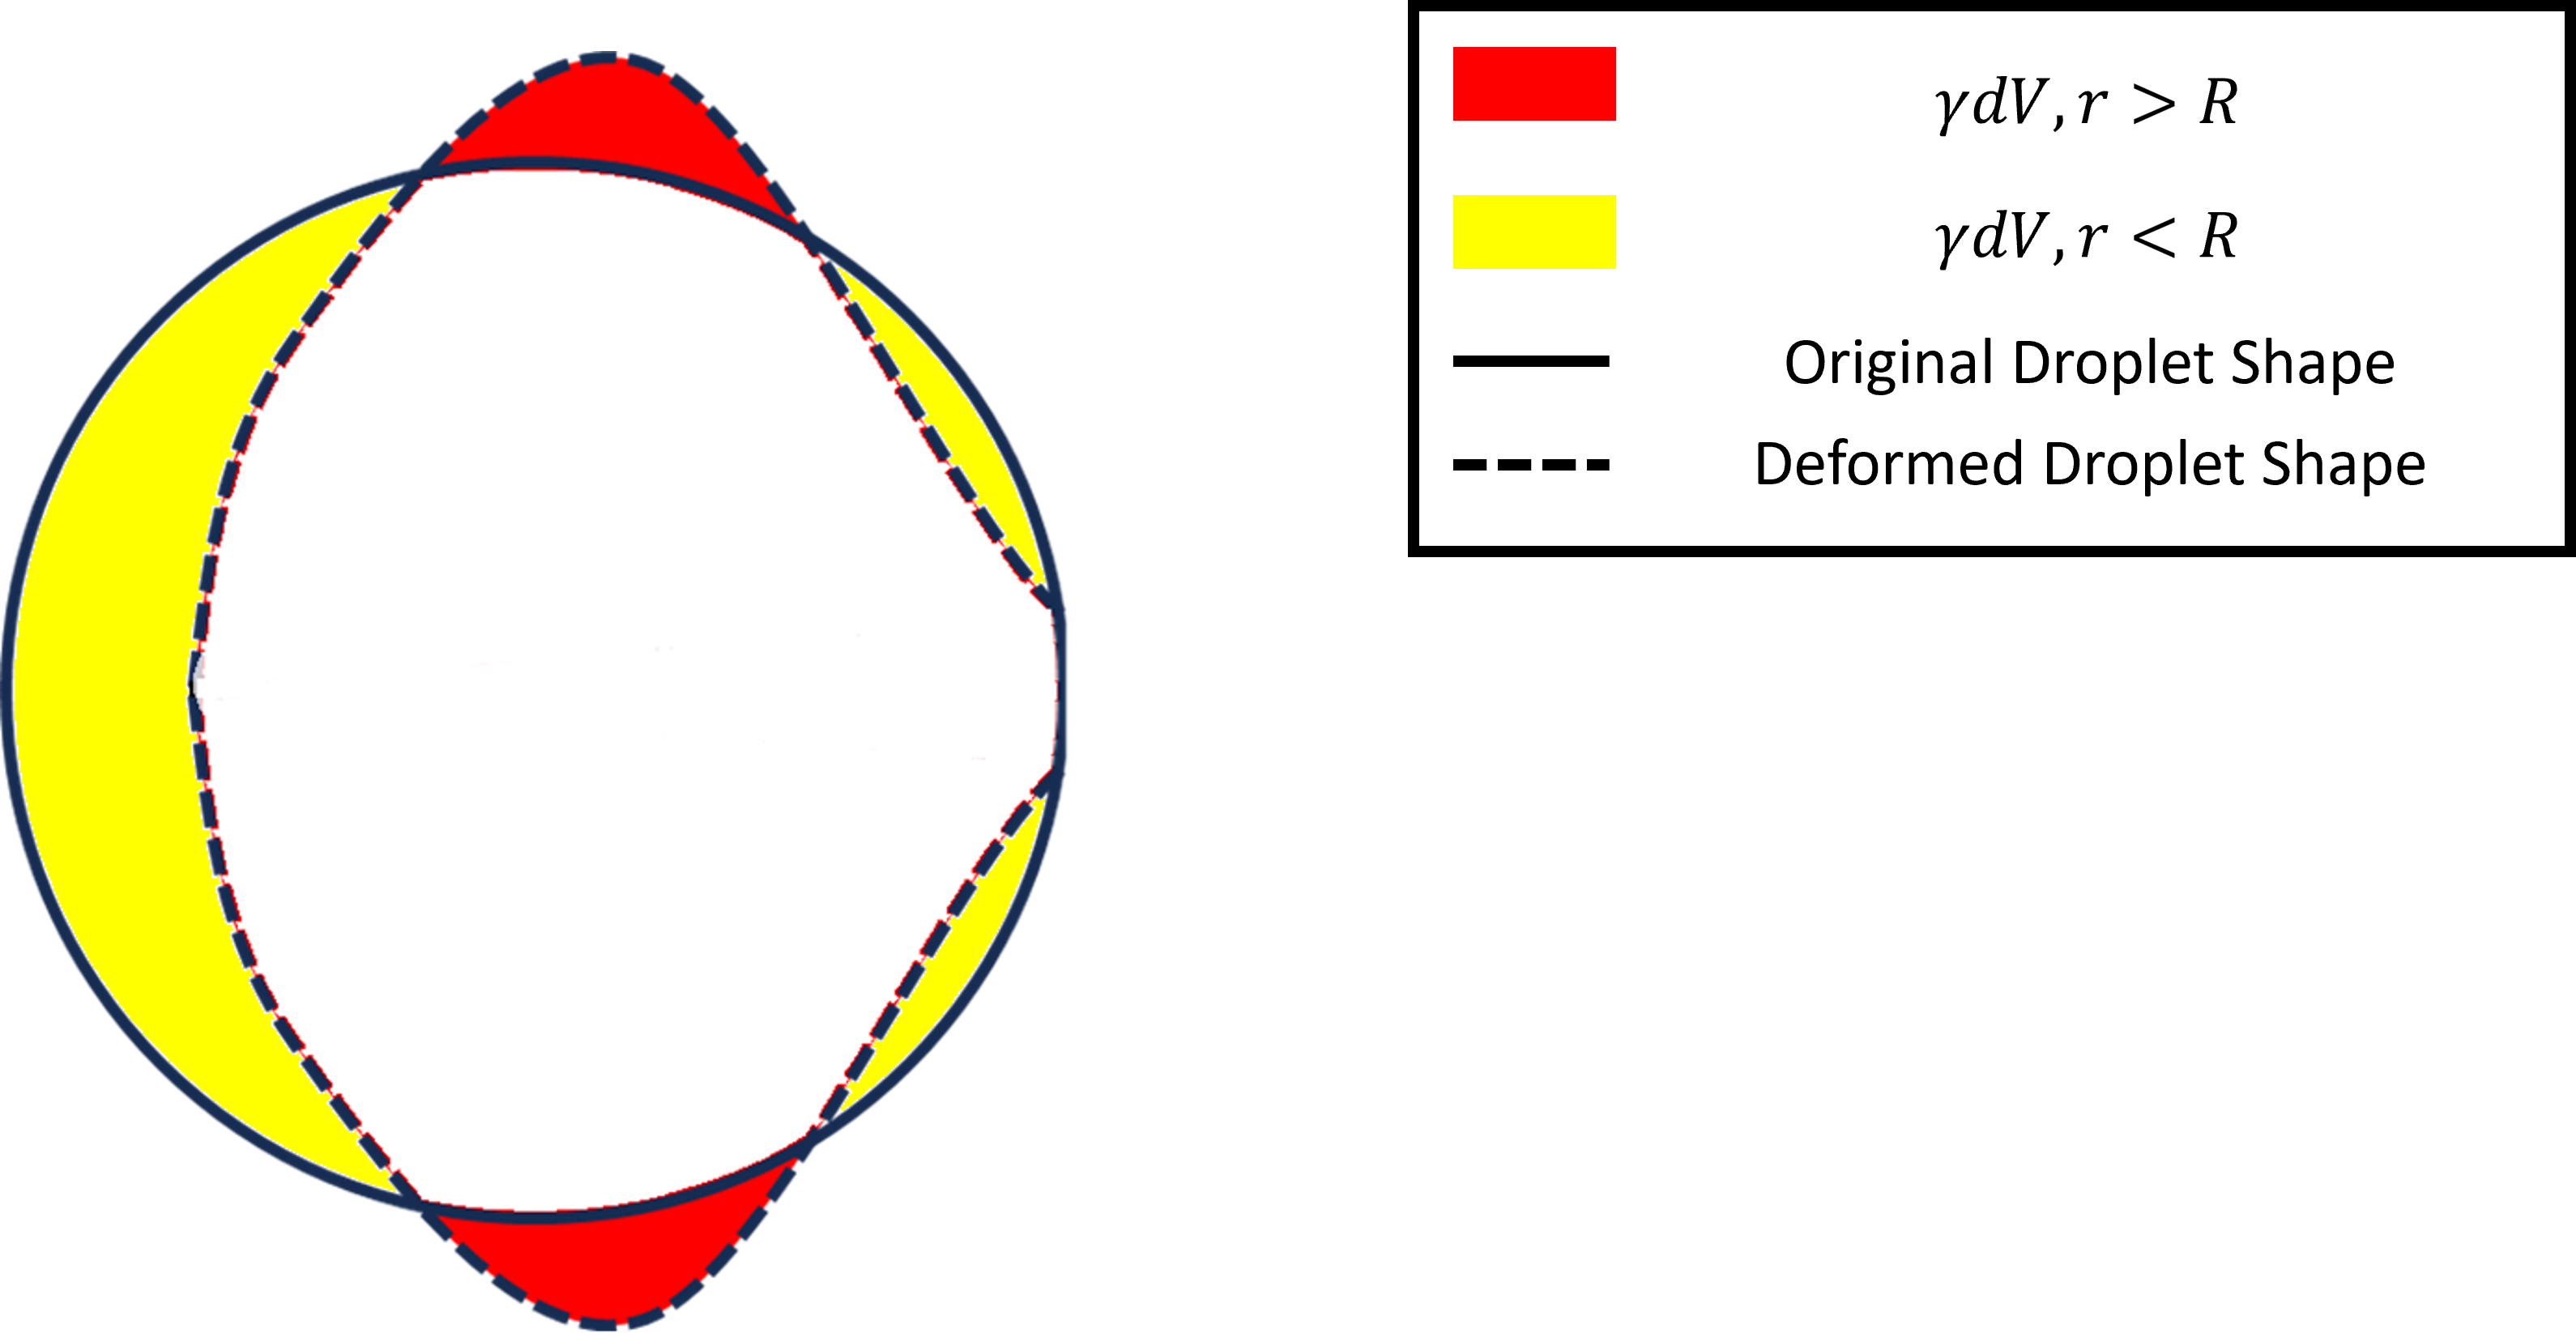
\includegraphics[width=0.8\linewidth]{Figures/nonsphere_diagram.png}
%     \caption{Shown is a diagram of the original droplet shape (solid line) and a deformed droplet shape (dashed line). Regions highlighted in red show the $r > R$ contribution to Equation \ref{eq:non-sphere}, regions highlighted in yellow show the $r<R$ contribution to Equation \ref{eq:non-sphere}}
%     \label{fig:non-sphereDiagram}
% \end{figure}

\subsection{Material Laws of Air and Water, and Water Vapor}
\label{sec:materials}
Air was modeled via the Ideal-gas Law, $P = \rho R T$. The water vapor generated from the cavitation model was also modeled as an Ideal-Gas. The liquid water was modeled with a second-order compressible equation-of-state \cite{hamilton2008nonlinear},

\begin{equation}
    \rho - \rho_{0} = \left( p_{abs} - P_{0} \right) \left( \frac{1}{c_{0}^{2}} - \frac{\left( \beta - 1 \right) \left( p_{abs} - P_{0} \right) }{\rho_{0} c_{0}^{4}} \right)
    \label{eq:waterEOS}
\end{equation}

\noindent which was described for water by Esplin \cite{Esplin2016, esplin2016bulk}. Here, $\beta$ is the coefficient of nonlinearity, ($\approx$ 3.5 for water). the low-amplitude speed-of-sound, $c_{0}$, is derived from the nonlinear sound speed,


\noindent The advantage of second-order compressibility is the ability to capture nonlinear distortion in the pressure waves.

\subsection{Domain, Mesh, Initial, and Boundary Conditions}
\subsubsection{Virtual Shock Tube}
\label{sec:domain_mesh}
The simulation was set up as an axisymmetric virtual shock tube, a depiction of which is shown in Fig. \ref{fig:domain}. These dimensions were chosen to emulate a shock tube in the VASU Lab at UCF \cite{Briggs2024}. The droplet is initialized at the center of the virtual shock tube, and a moving normal shock is initialized upstream of the droplet such that it will interact with the droplet after some time. The initial and boundary conditions were parameterized such that only the ambient air conditions and the $M_{shock}$ need to be specified (shown in Figure \ref{tab:boundaryConditions_shockDrop}). Given these parameters, the moving normal shock equations and the isentropic flow equations \cite{john2006gas} are used to calculate the upstream conditions required to produce a shock at the given $M_{shock}$ and ambient air conditions.



\begin{figure}[htp!]
\centering
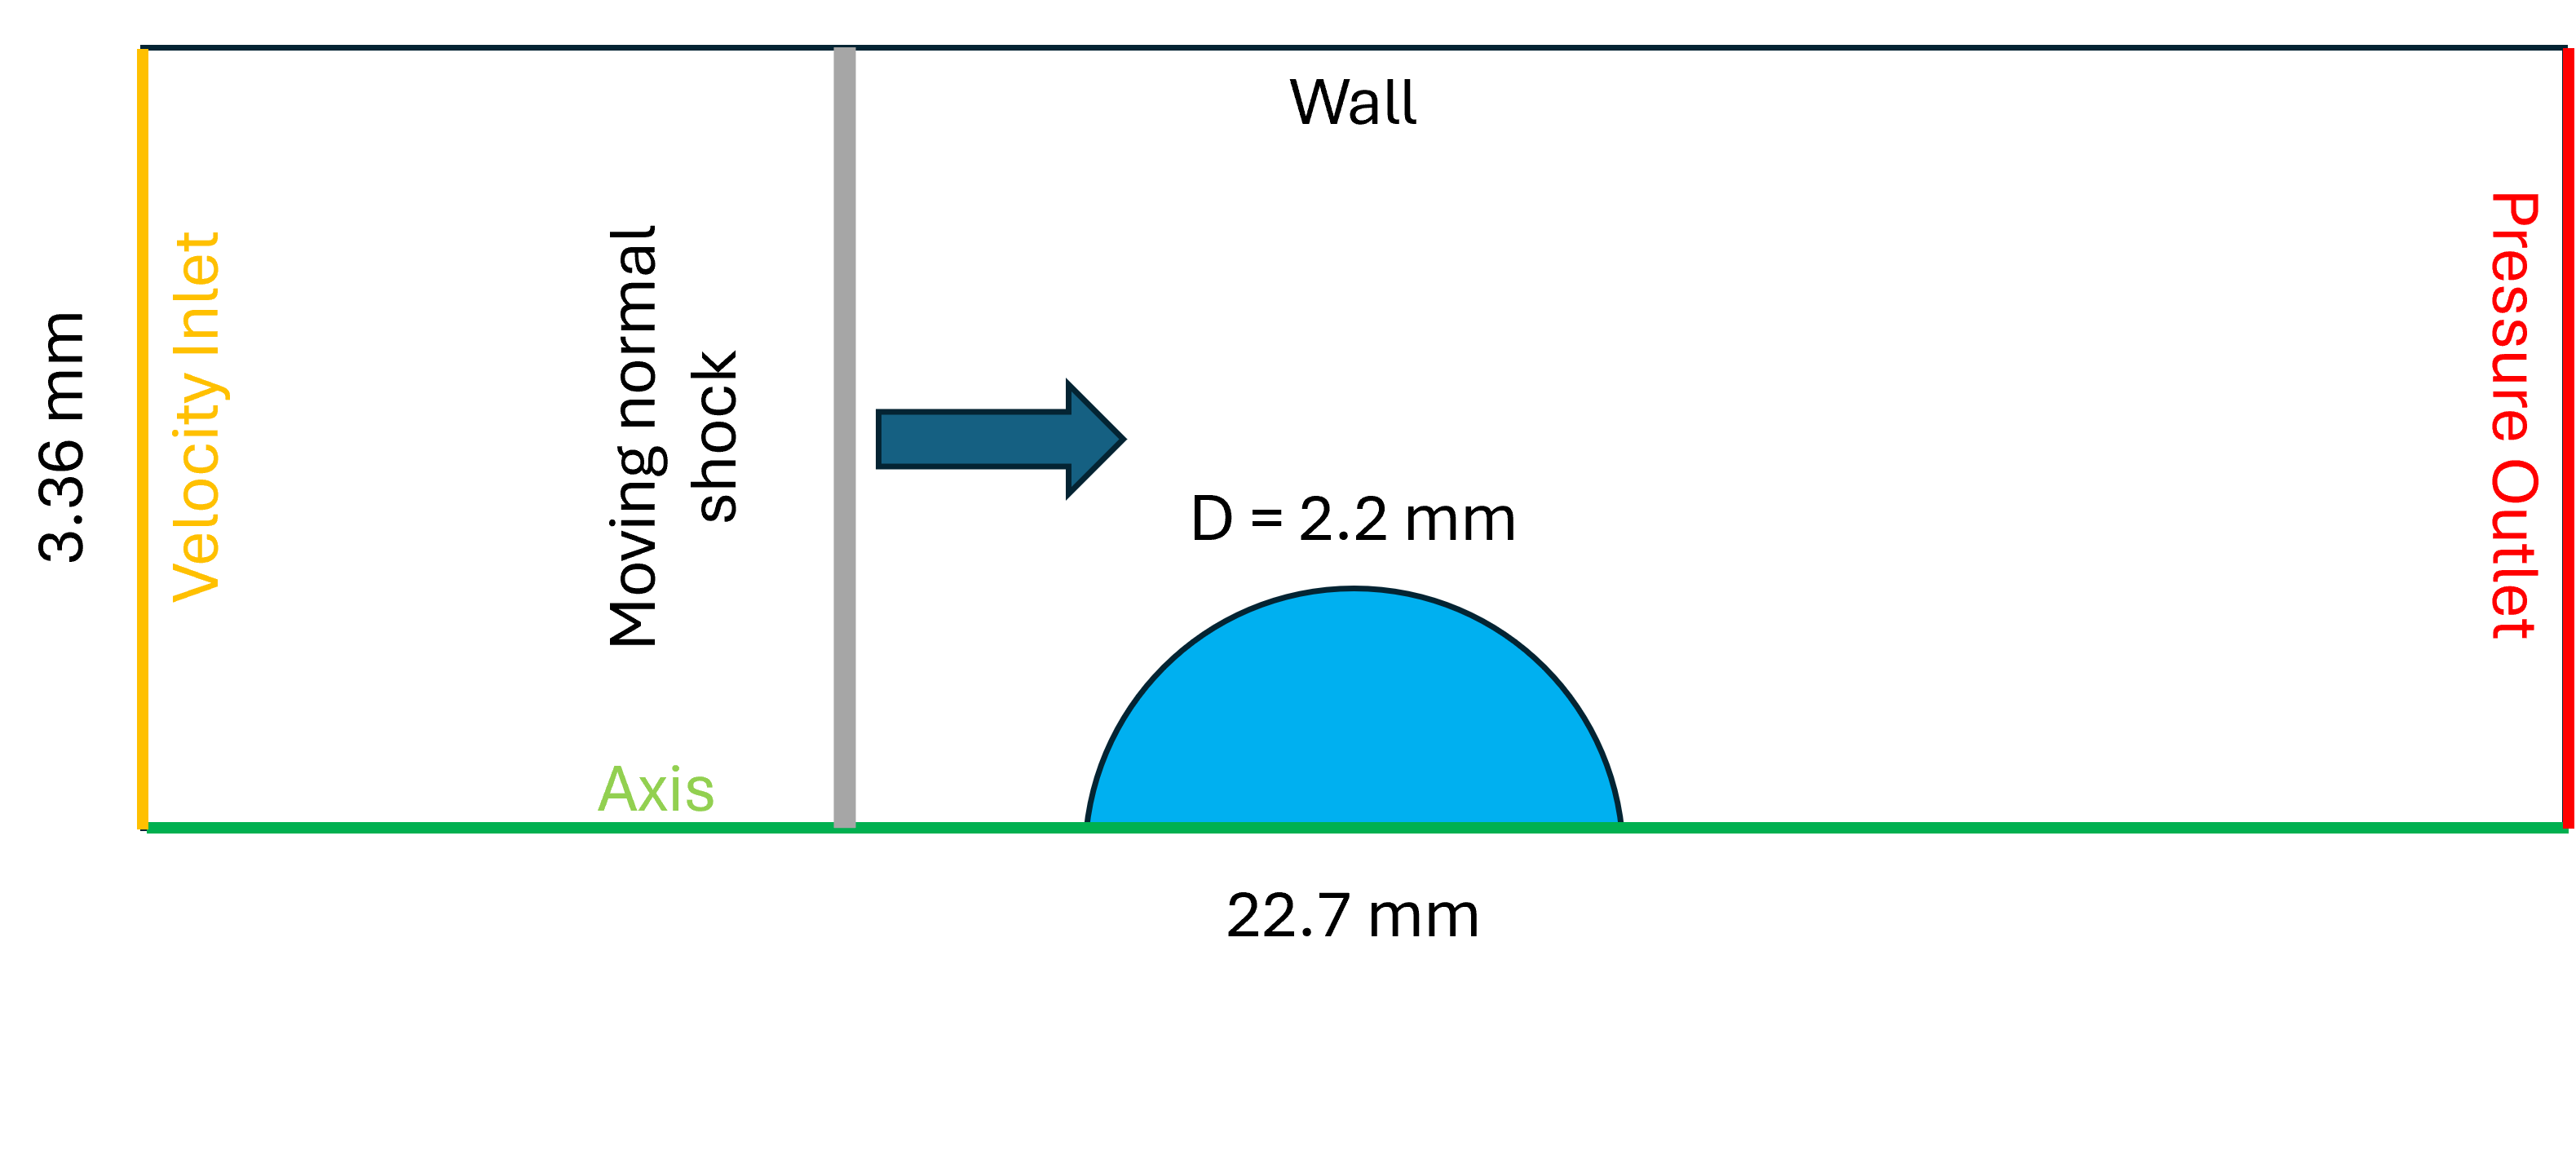
\includegraphics[width=.75\textwidth]{Figures/domain.png}
\caption{Virtual shock tube domain with labelled dimensions and boundaries.}
\label{fig:domain}
\end{figure}

\begin{figure}
\centering
    \begin{subfigure}[b]{\textwidth}
        \centering
        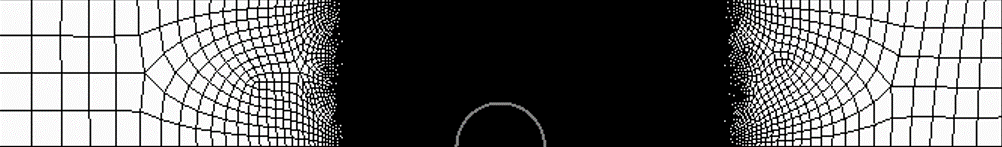
\includegraphics[width=0.8\textwidth]{Figures/mesh.png}
        \caption{}
        \label{subfig:mesh_zoomed_out}
    \end{subfigure}
        \begin{subfigure}[]{0.49\textwidth}
        \centering
        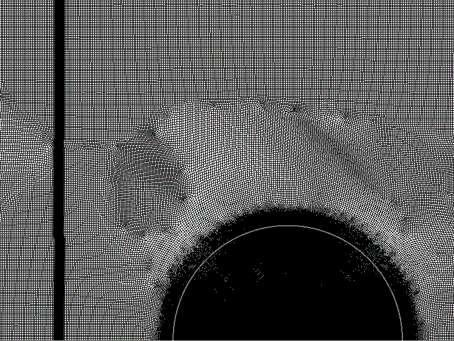
\includegraphics[width=\textwidth]{Figures/zoomed-in_mesh.png}
        \caption{}
        \label{subfig:mesh_shock}
    \end{subfigure}
        \begin{subfigure}[]{0.49\textwidth}
        \centering
        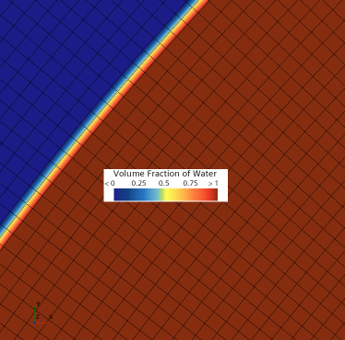
\includegraphics[scale=0.55]{Figures/mesh_alignment.png}
        \caption{}
        \label{subfig:mesh_alignment}
    \end{subfigure}
\caption{ (\ref{subfig:mesh_zoomed_out}) Image of the numerical mesh showing coarsening far away from the droplet, (\ref{subfig:mesh_shock}) a zoomed-in image of the droplet and shock with mesh edges overlayed on a numerical schlieren image, and (\ref{subfig:mesh_alignment}) an image zoomed in on the air-droplet interface showing the initially aligned mesh at the interface.}
\label{fig:dropMesh}
\end{figure}

%\renewcommand{\arraystretch}{1.75}
\begin{table}
\caption{\label{tab:boundaryConditions_shockDrop} Summary of Boundary Conditions (Pressure values with respect to reference pressure)}
\centering
\begin{tabular}{lcc}
\hline
Label & Boundary Condition& Value (Units)\\\hline
Velocity Inlet & Velocity & $\frac{2a_{air}M_{shock}}{\gamma +1} \left( 1- M_{shock}^{2}\right) $(m/s) \\
-& Temperature & $ T_{air}\left[ 1 + \frac{\gamma - 1}{2 a_{air}^2} \left( 2sV - V^{2} \right)  \right]$ (K)\\
Pressure Outlet & Pressure& 101,000 (Pa)\\
-& Temperature & 295 (K) \\
Wall& No-slip& -\\
\hline
\end{tabular}
\end{table}

\subsubsection{Description of Numerical Mesh}
\label{subsubsec:mesh}
The finite-volume representation of the virtual shock tube is captured by unstructured quadrilateral control-volumes, as shown in Figure~\ref{fig:dropMesh}. Figure~\ref{fig:dropMesh} also shows the coarsened cells upstream and downstream of the droplet. Coarsening far away from the droplet was done to increase computational efficiency without affecting the result. The mesh is refined near the droplet. A fine mesh at the air-water interface is important to resolve surface tension and to prevent interface smearing. A fine mesh within the droplet is necessary to capture potential regions of cavitation.





% \section{Particle-Wall Impact}
% The methodology for a droplet impinging on a wall is incredibly similar to that shown in Section \ref{sec:shock-droplet_method}. The physics and numerics are set up identically, except for the following:

% \begin{enumerate}
%     \item There is no shock in the domain (If it is a high-Mach flow, the droplet would've already passed through the vehicle's bow shock)
%     \item A solid region is modeled downstream of the droplet.
% \end{enumerate}

% \subsection{Domain and mesh}

% The color-coded and labeled domain is shown in Figure \ref{fig:wallDropDomain}. The major differences between this domain and that shown in Section \ref{sec:shock-droplet_method} is the lack of an initial shock, as well as a solid wall region. The boundary conditions are summarized in Table \ref{tab:wallDroplets}

% \begin{figure}[htp!]
%     \centering
%     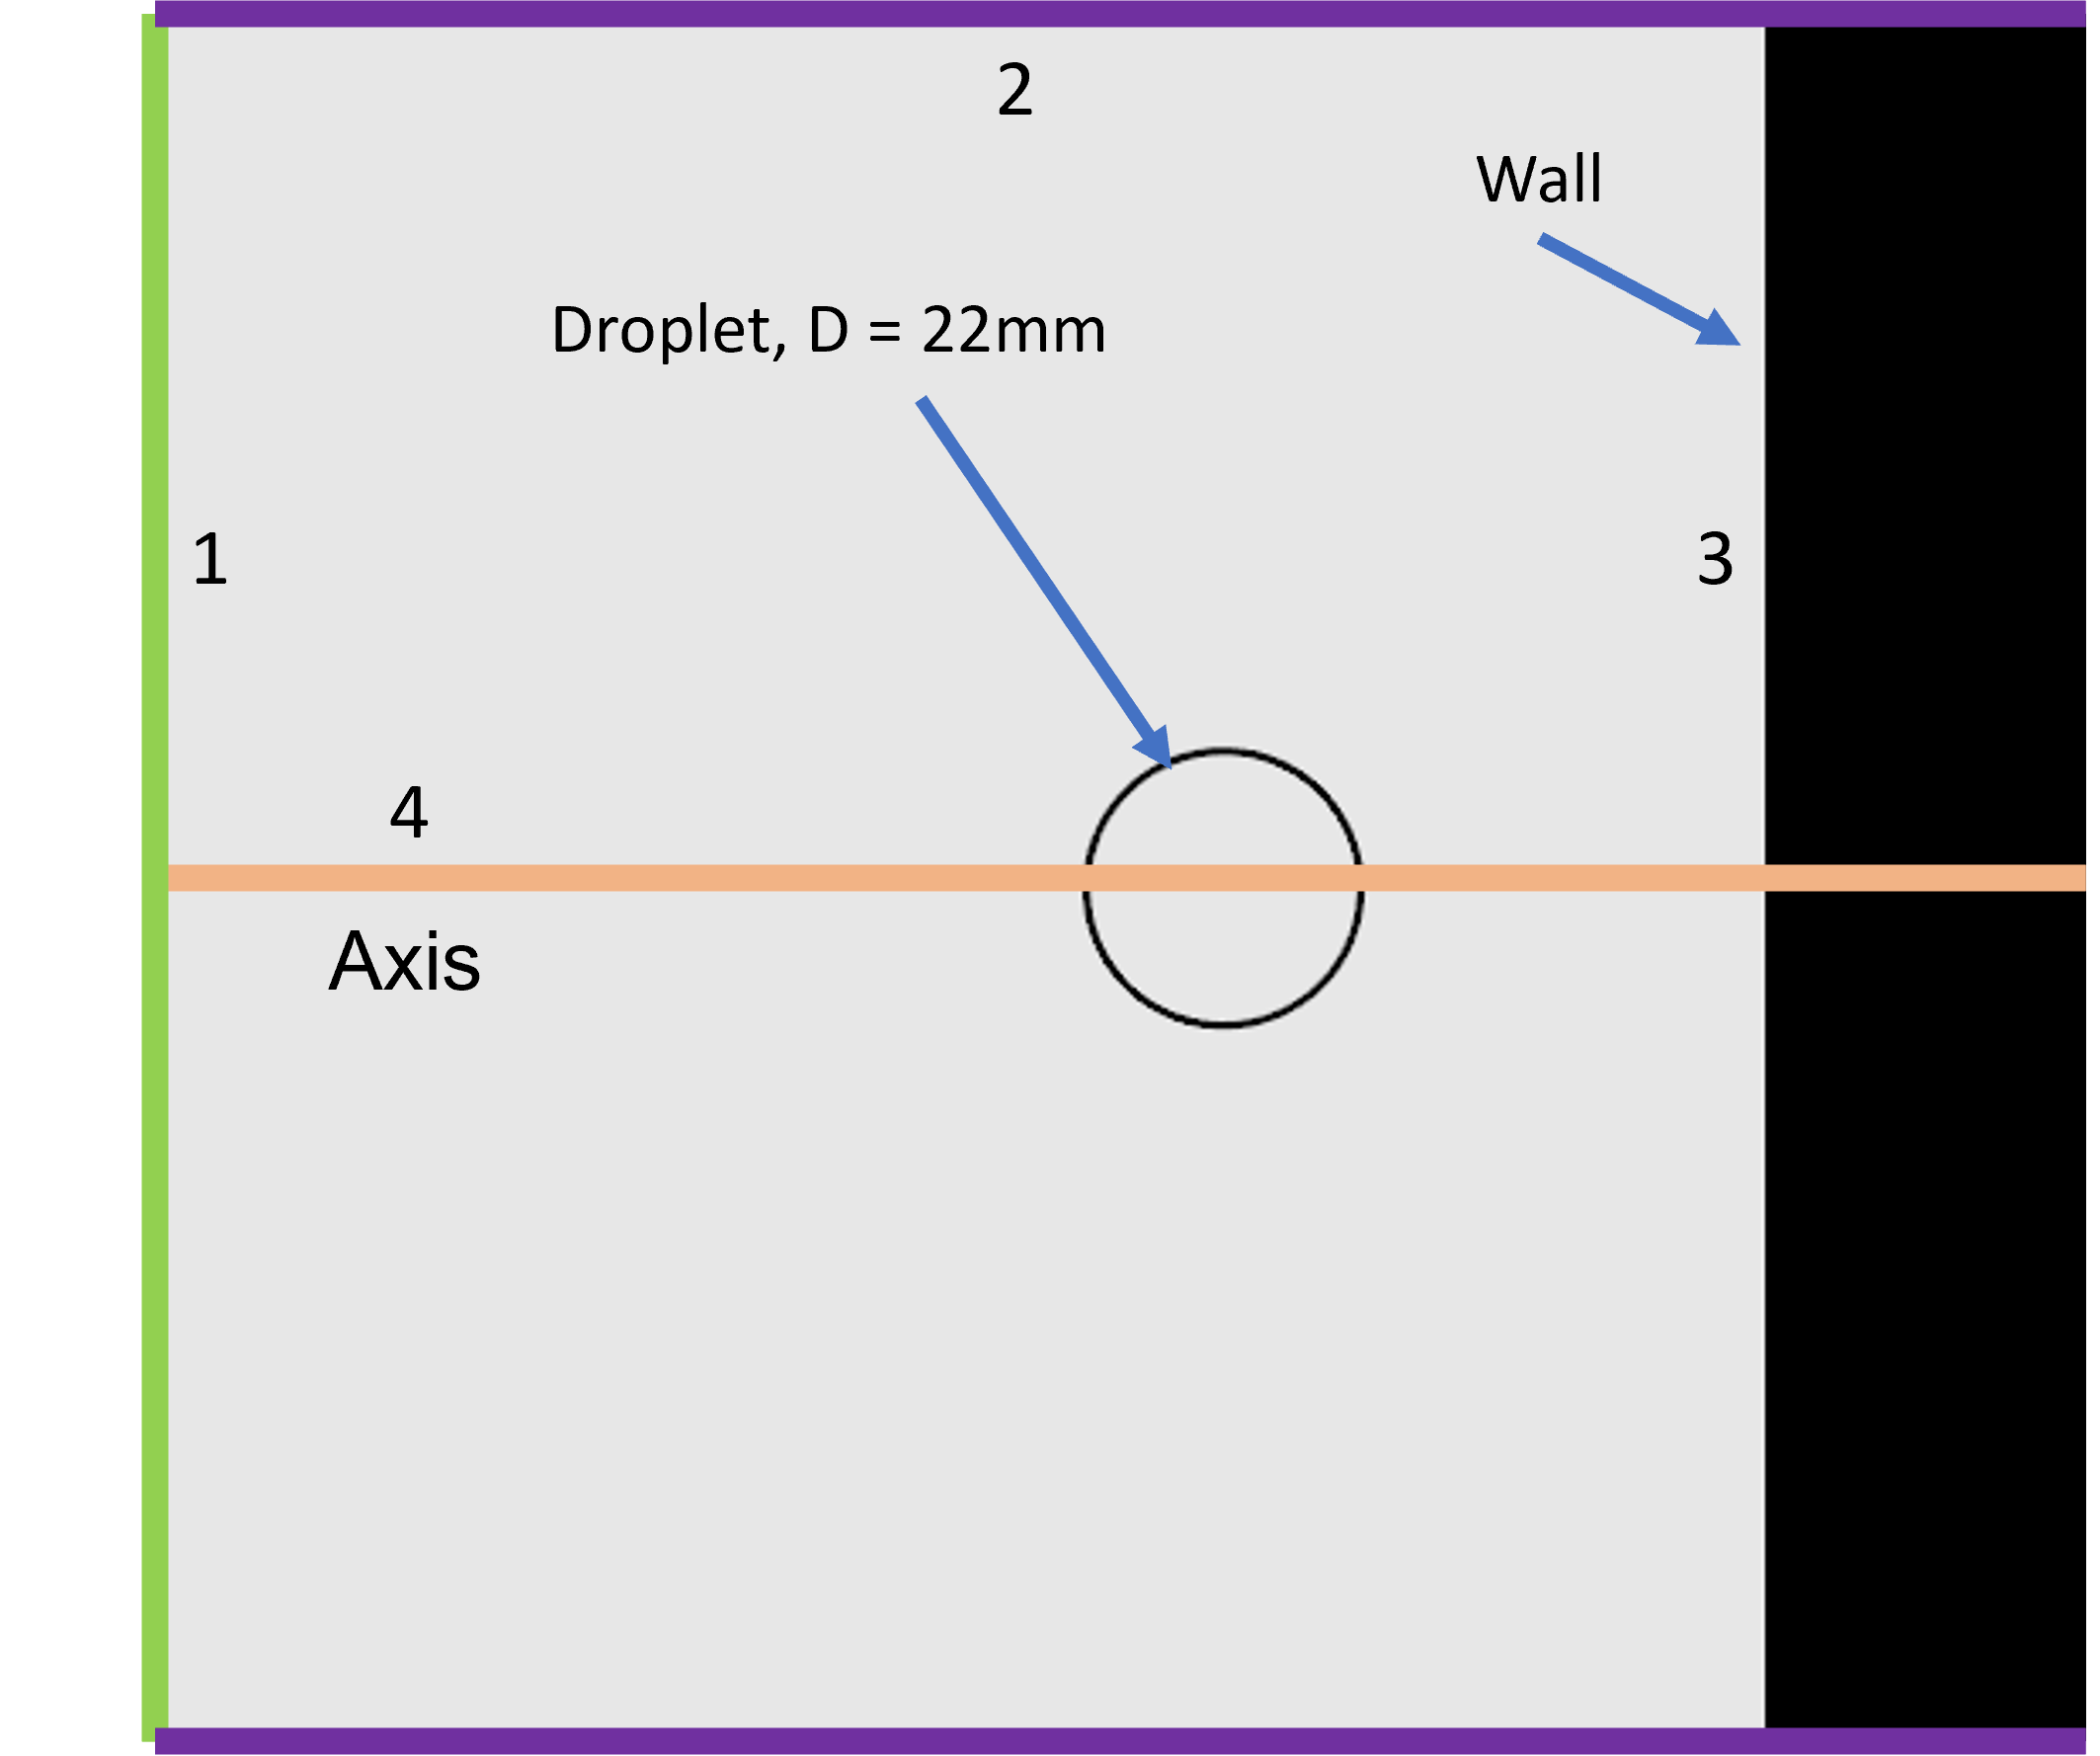
\includegraphics[width=.5\textwidth]{Figures/wallImpact_numerical_schliren.png}
%     \caption{Labaled and color-coded domain for the wall impingement simulation model}
%     \label{fig:wallDropDomain}
% \end{figure}

% \begin{table}
% \caption{\label{tab:wallDroplets} Summary of Labeled Boundary Conditions for wall impingement simulation domain}
% \centering
% \begin{tabular}{lcccccc}
% \hline
% Label & Boundary Condition& Value (Units)\\\hline
% 1& Stagnation Inlet & -----\\
% -& Total Pressure & 12.6 MPa\\
% -& Temperature & 2655 K\\
% 2& No-slip Wall & -----\\
% 3& Resolved Wall & -----\\
% 4& Axis & -----\\
% \hline
% \end{tabular}
% \end{table}

% The meshing for this work is also similar to that in Section \ref{sec:shock-droplet_method}. However, a new refinement region is introduced to capture any droplet spread/spray. The wall region is also meshed coarsely with quad cells. A diagram of the mesh is seen in Figure \ref{fig:wallDropMesh}

% \begin{figure}[htp!]
%     \centering
%     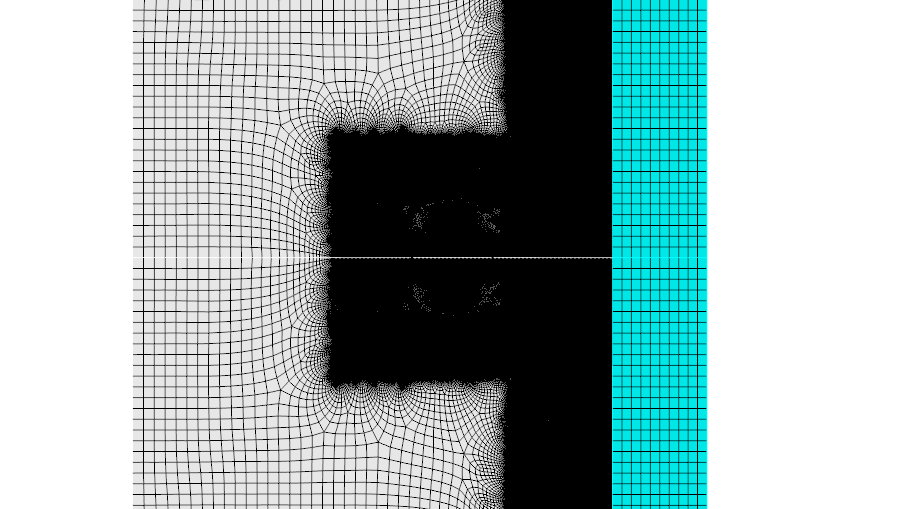
\includegraphics[width=.75\textwidth]{Figures/wallImpact_numerical_schliren_mesh.png}
%     \caption{A diagram of the mesh for the wall impingement simulation}
%     \label{fig:wallDropMesh}
% \end{figure}

% \subsection{Data Collection Methods}

% The same passive scalars described in Section \ref{sec:shock-droplet_method} are used here, but in different context. The shock-tracking passive scalars are still used to track the shock. However, now the shock is expected to appear inside the droplet as the droplet impacts the wall. The primary difference is that the shock propagates radially from the initial point of contact, as opposed to the normal shock transmitted in the shock-droplet interaction case.

% The diffusive passive scalar used to track secondary droplets is used here as well, this time to track the droplet splashing after wall impact. Data from this passive scalar is used to characterize the splashing.

% The shape characterization methods, mainly the sphericity and ellipticity calculation is used here as well to track the droplet spread as it impacts the wall.

% Pressure and shear forces will be calculated in the solid wall region to elucidate potential damage caused by the droplet impact. An important note here is that, for this to work, the simulation domain must be expanded from axisymmetric to 3D, because the solid stress solver in Star-ccm+ requires a 3D mesh. To maintain 

% \section{CMAS/TBC Interactions}
% \label{sec:CMAS/TBC_method}
% The simulation methodology is explained in previous work \cite{Cavainolo2023, Cavainolo2022} and will be summarized here. 

% \subsection{Governing Equations}
% The simulation methodology is explained in previous work \cite{Cavainolo2023, Cavainolo2022} and will be summarized here. The first step in simulating the infiltration of CMAS was to ensure the VOF method is a valid approach for capturing the melting-solidification of a CMAS particle. A mesh independence study was conducted in previous work \cite{Cavainolo2022}, and it is shown that melting particles between the solidus and liquidus temperatures of CMAS can be accurately resolved with the VOF method. For multiphase physics, the Eulerian Multiphase Volume-of-Fluid method was used to simulate the interactions between the two Eulerian phases, air, and CMAS.  Modeling surface tension properly is critical as the infiltration is driven mostly by capillary forces. The governing equations for the VOF method in Star-CCM+ ver. 18.02.008-R8 \cite{starccm} are shown in a finite-volume formulation and include the the Conservation of Mass,

% \begin{equation}
% \label{consMass:equation}
%     \frac{\partial}{\partial t}\int_{V}\rho dV+\ \oint_{A}{v\bullet d\ A}=\ \int_{V}\left(S\right)dV\ ,\ S=\ \sum_{i}{S_{a_i}\rho_i},
% \end{equation}

% \noindent the Conservation of Momentum,

% \begin{eqnarray}
% \label{consMomentum:equation}
%     &&\frac{\partial}{\partial t}\int_{V}\rho vdV+\oint_{A}{\rho v\times v}\bullet\ dA \nonumber\\
%     &&=\oint_{A}{\rho I\bullet d\ A}+\oint_{A}{T\bullet d\ A}+\int_{V}\rho gdV\ \\
%     &&+\int_{V}{f_bdV}-\sum_{i}\int_{A}{a_i\rho_iv_{d,i}\times v_{d,i}dA}\nonumber
% \end{eqnarray}


% \noindent and the Conservation of Energy,

% \begin{eqnarray}
% \label{consEnergy:equation}
%    &&\frac{\partial}{\partial t}\int_{V}\rho EdV+\oint_{A}\left[\rho Hv+p+a_i\rho_i{H_iv}_{d,i}\right]\bullet dA=\nonumber \\
%    &&=-\oint_{A}{{\dot{q}}^{\prime\prime}\bullet d A} \\
%    &&+\oint_{A}{T\bullet v d A}+\int_{V}{S_EdV}+\ \int_{V}{f_bdV}.\nonumber
% \end{eqnarray}


% \noindent Equations 3-5 couple to the Eulerian Multiphase VOF Transport Equation which is formulated as follows 

% \begin{eqnarray}
% \label{VOFtrans:equation}
%     &&\frac{\partial}{\partial t}\int_{V}a_{i}dV+ \oint_{A}a_{i}v\cdot dA\nonumber\\
%     &&=\int_{V}\left(S_{a_{i}}-\frac{a_i}{\rho_i}\frac{D\rho_{i}}{Dt}\right)dV\\
%     &&-\int_{V} \frac{1}{\rho_{i}}\nabla\cdot \left(a_{i}\rho_{i}v_{d,i}\right)dV\nonumber
% \end{eqnarray}

% \noindent In these equations, the subscript i denotes a particular phase (in this case, air or CMAS), $a_{i} = V_{i}/V$ is the volume fraction of a particular phase, and $S_{a_{i}}$ is a source term defined by the initialization of the phases. The VOF method implements a technique called High-Resolution Interface Capturing (HRIC). HRIC imposes a Courant number limit (i.e. Co = 1.0), and if the Courant number is exceeded, then the HRIC scheme reverts back to a standard upwind scheme, which results in a smeared interface. This smeared interface can be corrected by implementing temporal subcycling. The general idea of temporal subcycling is shown in Equation \ref{eq:GeneralTempSubCycle}, where the right-hand side of the equation is a single source term that combines the right-hand side contributions from Equation \ref{VOFtrans:equation}. 

% \begin{eqnarray}
% \label{eq:GeneralTempSubCycle}
%     &&\alpha^{n+\Delta t}V - \alpha^{n}V + \int_{t^{n}}^{t^{n+\Delta t}}( \ \sum_{A}\alpha_{f}(s) v \cdot da)\nonumber\\
%     &&=\int_{t^{n}}^{t^{n+\Delta t}}(S(\alpha (s),...)ds
% \end{eqnarray}


% \noindent In this work, an implicit multi-stepping version of this temporal subcycling is employed, which gives an unconditionally stable solution, and a sharp interface is achieved if $\frac{CFL}{N_{imp}} \leqslant 0.5 $. The sub-iterations calculated with Equation \ref{eq:implicitMultiStep1} are summed up to get the overall contribution for the whole time step.

% \begin{eqnarray}
% \label{eq:implicitMultiStep1}
%     &&\alpha_{i+1}V - \alpha_{i}V + \tau( \ \sum_{A}\alpha_{f,i+1}(\tau) v \cdot da) \nonumber \\
%     &&=\tau(S(\alpha^{n+\Delta t},...) ~ for~ i = 1, 2, ..., N
% \end{eqnarray}

% A drawback of using the VOF method for the infiltration is the very small time steps required to resolve the CMAS infiltration. So, adaptive time-stepping combined with sub-iterations was used to balance computational speed and accuracy. A free-surface condition was enforced so that the Courant number ($Co = \frac{u \Delta t}{\Delta x}$) at the interface was around 1.0. Such a criterion is often demanded to limit the interfacial motion to only a cell. The VOF method requires the use of a segregated solver (i.e. the energy equation is solved in a separate system of equations). This solver is second-order accurate in space, and first-order accurate in time. However, the lower-order time accuracy is offset by the implicit multi-stepping in the segregated VOF solver, described in Equations \ref{eq:GeneralTempSubCycle} - \ref{eq:implicitMultiStep1}. 

% \subsection{Solidification Model}
% \label{sec:solidmodel}
% Solidification is treated in the following way in Star-CCM+'s implementation of the VOF method \cite{starccm}

% \begin{equation}
%     \alpha^{*}_{s} = \begin{cases}
%     1 & T^{*} < 0 \\
%     f(T^{*})& 0<T^{*}<1 \\
%     0& 1 < T^{*}
%     \end{cases},
%     \label{eq:solidificationModel}
% \end{equation}

% \noindent where
% \begin{equation}
%     T^{*} = \frac{T - T_{solidus}}{T_{liquidus} - T_{solidus}}
% \end{equation}.

% \noindent latent heat of fusion, $h_{fusion}$ is also taken into account in the model, where

% \begin{equation}
%     h_{is}^{*} = h_{is} + \left( 1 - \alpha_{s}^{8}\right)h_{fusion}
% \end{equation}

% \noindent A flow-stop submodel is also employed to stop the fluid flow in the cells that have reached a particular solid threshold (the flowability threshold). In order to maintain numerical stability in the solution of the continuity equation, the density in the stopped cells must be held constant, which is achieved with the flow-stop mass compensation option.  

% \subsection{Geometry, Mesh, and Boundary Conditions}

% Four different geometries were created for this study. Firstly, a planar micro-channel, represented by a 2D plane extending infinitely into the z-direction. The planar channel's purpose is to serve as a benchmark; a case that allows the numerical methods in this model to be compared to analytical models for capillary flow. For similar reasons, a circular pipe was set up both as an axisymmetric domain and a full 3D domain, and a full 3D concetric pipe was created. 

% Once the three geometries above were benchmarked, their results were compared to a fourth geometry, a feathery micro-channel. This feathery micro-channel was created by scientists at DLR \cite{Sirigiri2018} and imported into Star-ccm+ as an infinite 2D plane, shown in Figure \ref{dimensions}. Where the feathery pattern shown on the right is repeated downward until the TBC column is 200 $\mu m$ deep. This is half the size of a typical TBC column. 

% The mesh is an unstructured trimmed-cell mesh. The effect of contact angle was captured using prism layers at the wall. Boundary conditions, and domain dimensions, are summarized in Figure \ref{dimensions} and Table \ref{tab:boundaryConditions}. The top of the domain is a stagnation inlet, and the bottom of the domain was set as a pressure outlet with a pressure smaller than the reference pressure. This pressure difference between the inlet and outlet was set up so that a pressure gradient pushes the CMAS downward. The sides of the domain are also set as pressure outlets. Conjugate heat transfer was considered by setting the TBC as a solid region, the walls of the TBC were prescribed a temperature gradient, ($\Delta T_{x}$), of -1 $K/\mu m$, such that the top of the coating is close to a typical operating temperature for an engine environment. The gradient is defined this way because a typical YSZ EB-PVD TBC is around 400 $\mu m$ deep, and manages to be around 400 K cooler at the bottom of the TBC than the top, such that the operating temperature is below the melting point of the materials used. It should be noted there is only a gradient in the x-direction, so any walls on the same x-plane will have a constant temperature, and any walls along the same y-plane will have a temperature that varies.

% The mesh can be seen in Figure \ref{Fig3}. The wall contact angle of the CMAS phase is expected to be somewhere between 40 and 60 degrees based on experiments \cite{Naraparaju2019}. These values are temperature dependent though. For simplicity, a constant wall contact angle of 67 degrees was used \cite{Naraparaju2019}.  


% The thermal gradient described above for boundary conditions was also used as the initial condition for both the fluid region and solid region, except for the CMAS particle, which had a variable starting temperature. The fluid domain's initial velocity was set such that there was a very small downward velocity. This is done because it helps with convergence in the first calculations in the simulation. The CMAS particle was set at 0.2 m/s downward to ensure a quick interaction with the TBC. The reference pressure is 1 atm. While it could potentially make more sense to use engine operating pressures for the simulation's reference pressure, this domain was set up to be more in line with experiments conducted by Naraparaju et al. \cite{Naraparaju2014, Naraparaju2017, Naraparaju2019} to ensure the comparison to experimental data is as accurate as possible. Gravity was also enabled to capture any infiltration effects from buoyancy. Turning on gravity also adds the Boussinesq Approximation to the energy equation to account for natural convection. However, the effects of natural convection do not dominate the flow.

% \begin{figure}[htp!]
% \centering
% 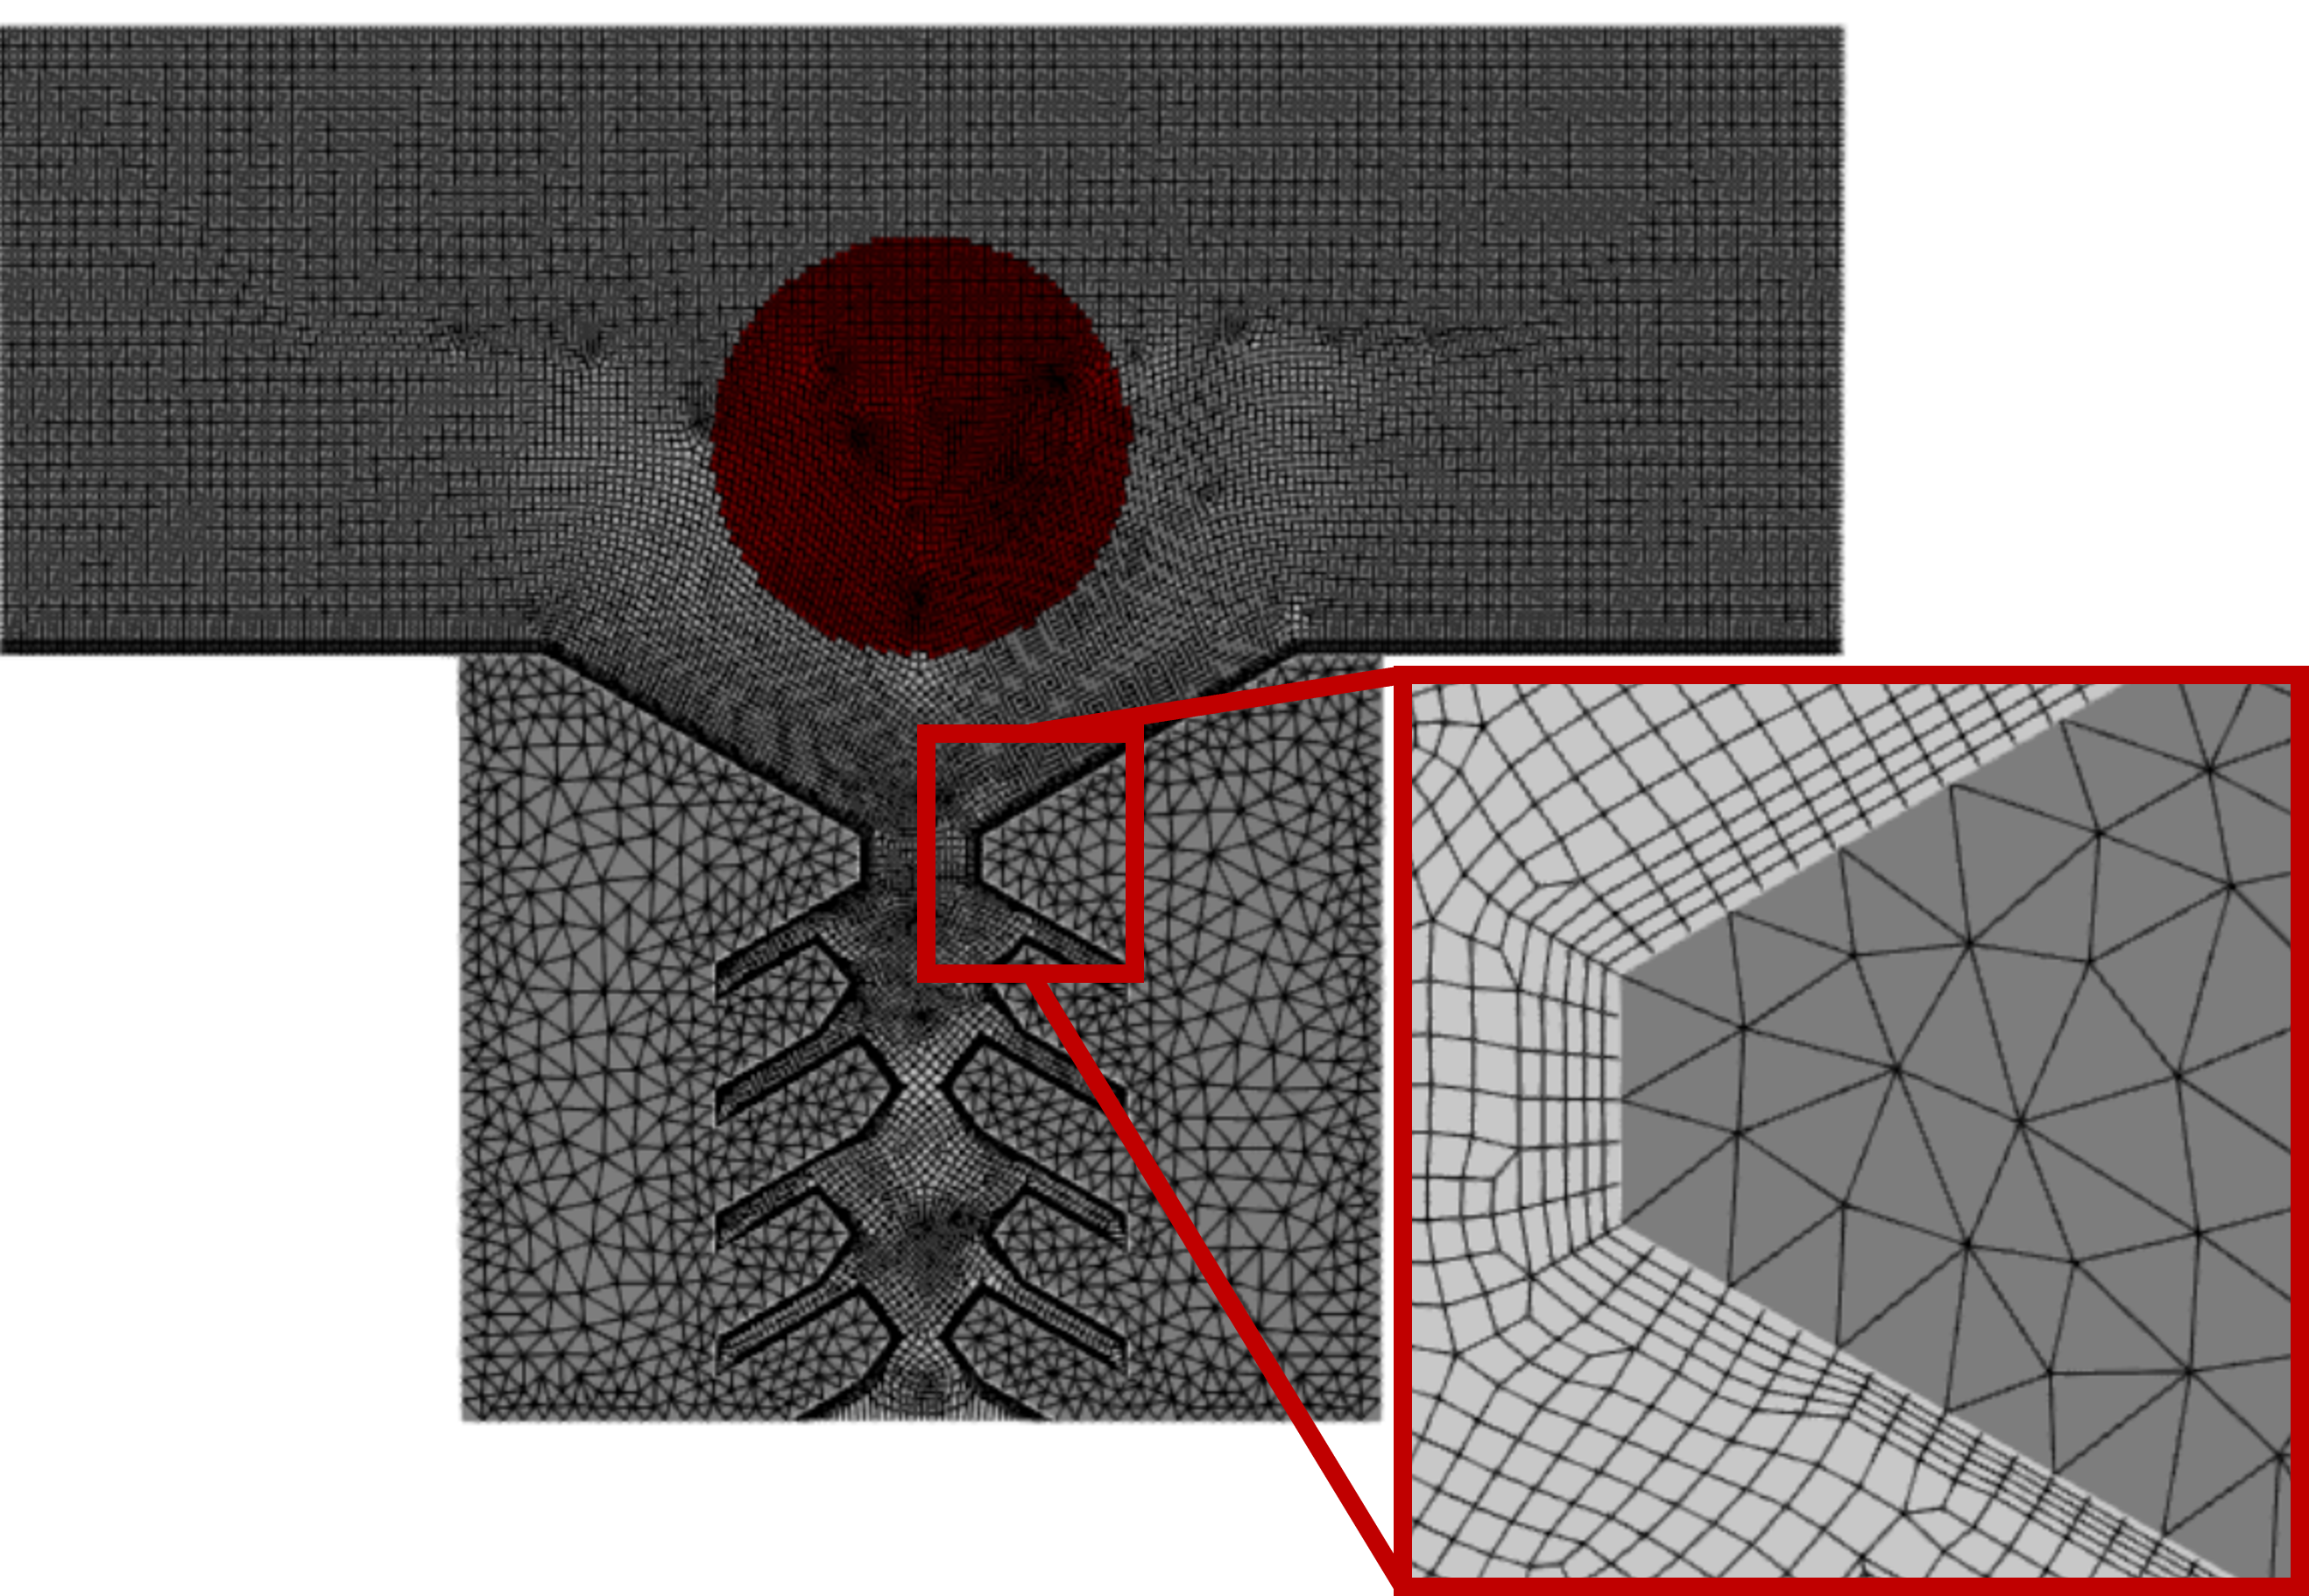
\includegraphics[width=\linewidth]{Figures/Fig3.png}
% \caption{Zoomed out mesh, and  mesh zoomed in around wall region}
% \label{Fig3}
% \end{figure}

% \begin{figure*}
% \centering
% 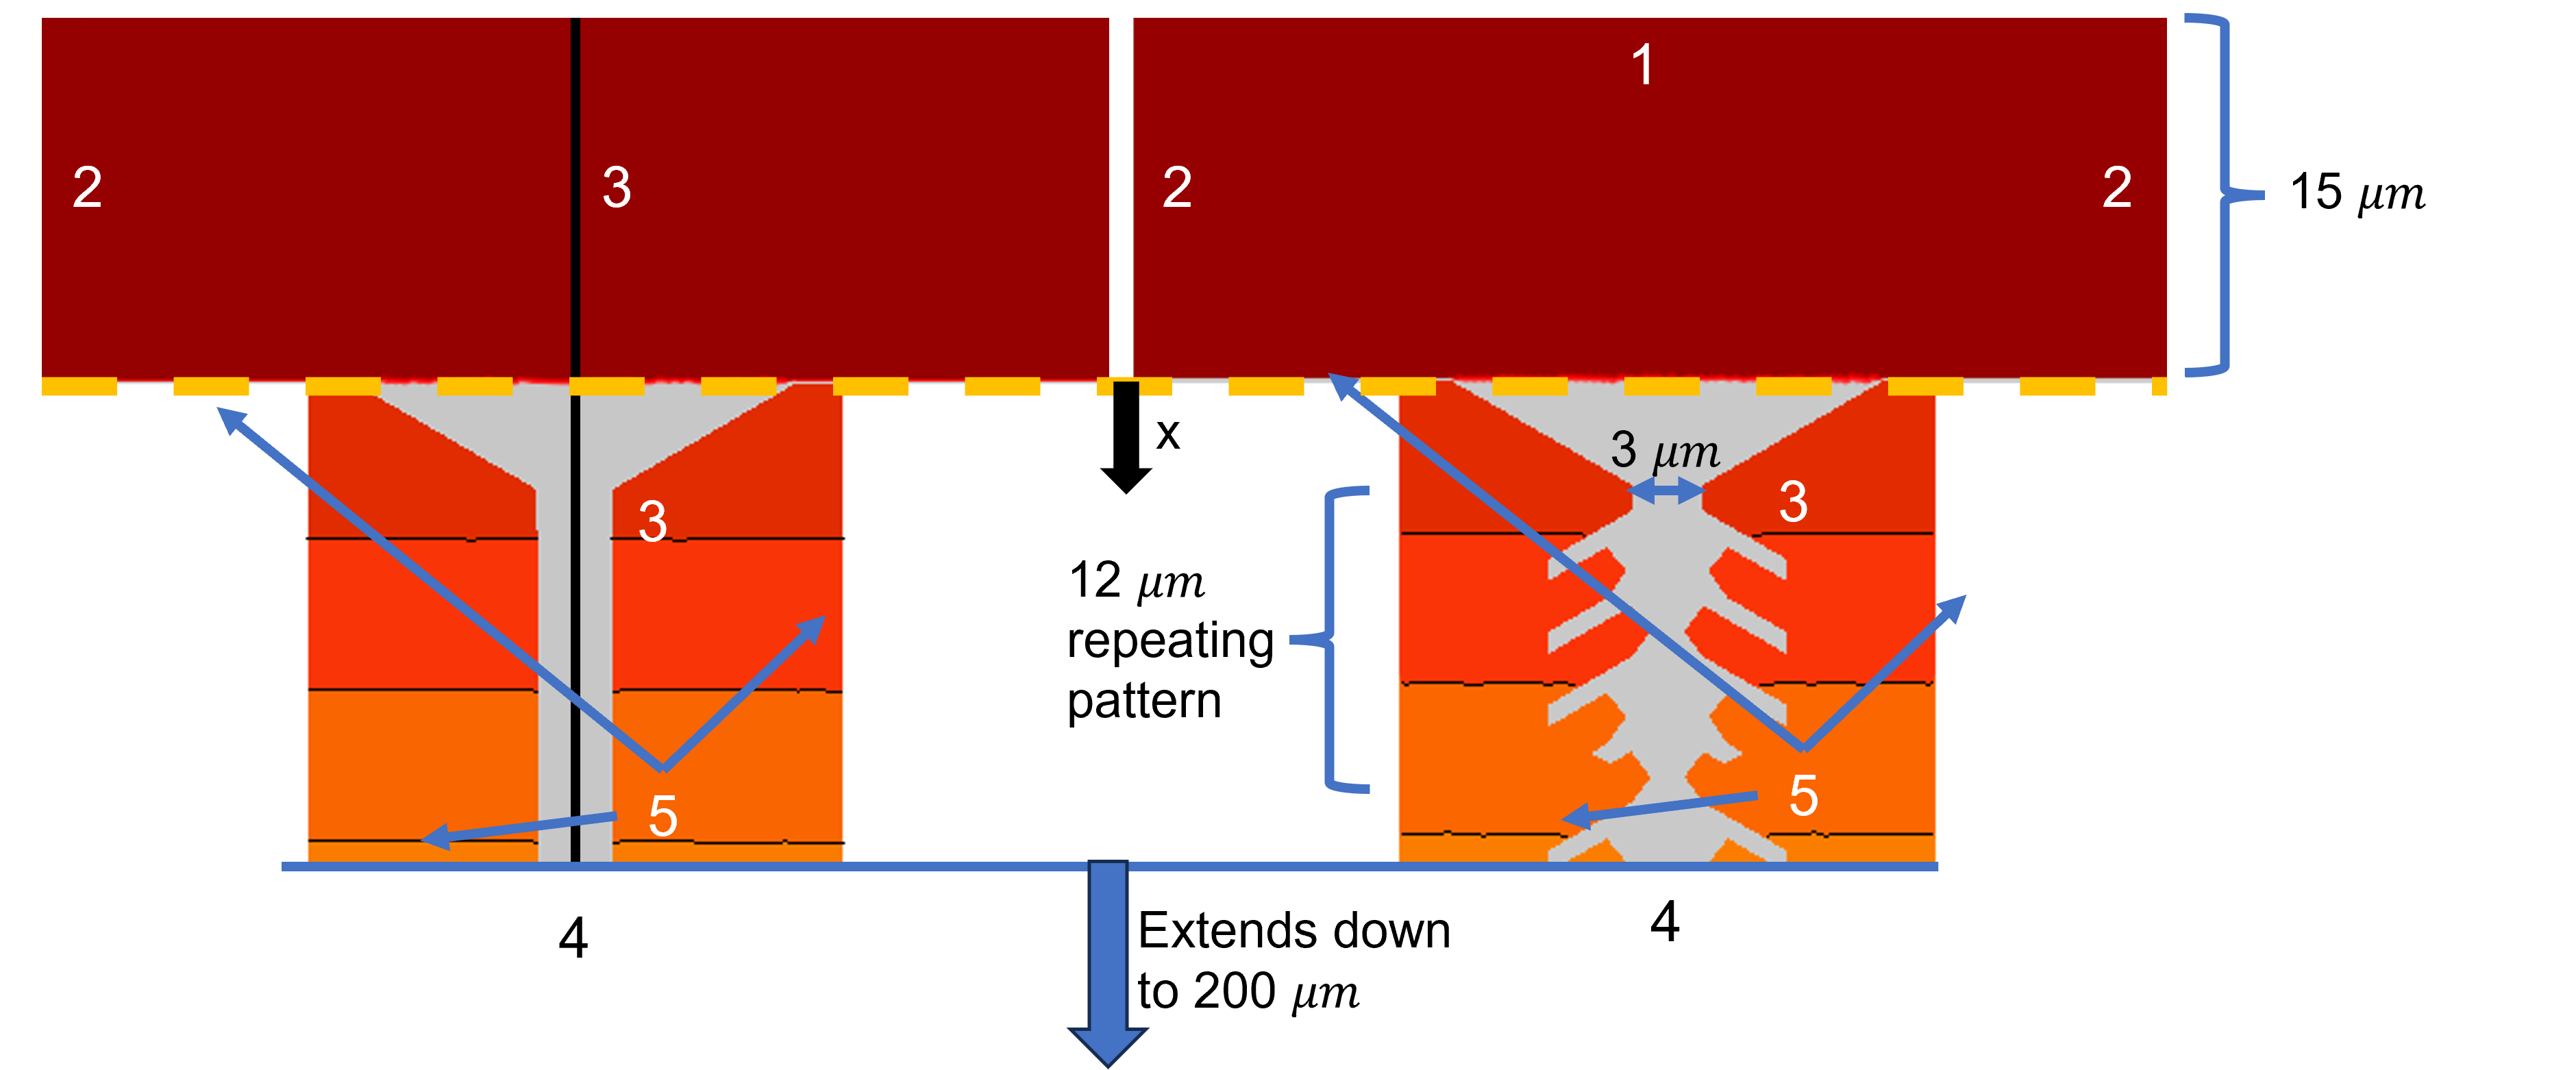
\includegraphics[width=0.9\linewidth]{Figures/dimensions.png}
% \caption{Geometry with labeled dimensions and boundary conditions}
% \label{dimensions}
% \end{figure*}



% \begin{table}[htp!]
% \caption{\label{tab:boundaryConditions} Summary of Labeled Boundary Conditions (Pressure values with respect to reference pressure $P_{ref} = 101325$ Pa)}
% \centering
% \begin{ruledtabular}
% \begin{tabular}{cccc}
% Label &Type& Boundary Condition& Value (Units)\\\hline
% 1& Inlet&Pressure & 3.0 $MPa$\\
% -& -&Temperature& $1530$ K\\
% 2& Inlet&Pressure& 3.0  $MPa$\\
% -& -&$T(x)$& 1530 -$\Delta T_{x}\times x$ (x in $\mu m$)\\
% 3& Symmetry&- & -\\
% 4& Oulet&Pressure& -50 $MPa$\\
% -& -&Temperature & $1324$ K \\
% 5& Walls&$T(x)$& 1530 -$\Delta T_{x}\times x$ (x in $\mu m$)\\
% \end{tabular}
% \end{ruledtabular}
% \end{table}

% \subsection{Air Phase and Porosity}
% The air phase was modeled as a constant-density fluid in this simulation. Thus, it is necessary to account for air getting trapped within the feather gaps as it would prevent the CMAS from infiltrating those gaps. To accomplish this, the interface between the fluid and solid regions was set as a porous boundary, only allowing air to escape. The rate at which air was allowed to escape was based on a user-defined external pressure, inertial resistance, and viscous resistance, which were 0 Pa (reference), 100 (dimensionless), and 1 m/s respectively. Hence, the air can escape the fluid domain at a maximum velocity of 0.01 m/s according to Eq. \ref{porous:equation} \cite{starccm}.

% \begin{equation}
% \label{porous:equation}
%     \Delta P = -\rho (\alpha |v_n| + \beta)v_n
% \end{equation}

% \subsection{Properties of the TBC and CMAS}
% \label{subsec:CMAS/TBCProp}
% Properties of both the CMAS and the TBC can affect the infiltration. Some of these properties are widely documented, such as thermal conductivity of the TBC \cite{Han2023}. Table \ref{tab:CMAS and TBC properties} shows the properties for both the CMAS and the TBC used in these simulations. Blank entries are properties not required by the models selected (in this case, for the solid TBC region).


\begin{table}
\caption{\label{tab:CMAS and TBC properties} Summary of thermal and physical properties of CMAS and TBC}
\centering
\begin{tabular}{lcccccc}
Property & CMAS& TBC\\\hline
Thermal Conductivity (W/m-K)& 1.15 \cite{Bakal2017} & tabular \cite{Han2023} \\
Specific Heat (J/kg-K)& 900 \cite{KAKUDA2015350} & tabular \cite{Han2023} \\
Density (kg/m$^3$)& 2690 \cite{BANSAL20153901}& 4800 \cite{KAKUDA20092583}\\
Dynamic Viscosity (Pa-s)& Polynomial \cite{Naraparaju2019}& -\\
Latent Heat of Fusion (J/kg)& $1.973x10^7$ \cite{Costa2019}& -\\
Surface Tension (N/m)& 0.4 \cite{Bravo2020}& -\\
\end{tabular}
\end{table}

% One important departure from previous work, however, is the use of the melting-solidification flow stop model to achieve a more accurate infiltration time. Here, a linear solidification curve is defined between the liquidus and solidus temperatures (1503 K and 1523 K respectively). The solid fraction of a particular cell is calculated as described in Section \ref{sec:solidmodel}.

% % \subsection{Modifications to the Governing Equation for Capillary Flow in a planar micro-channel}

% % For analytical benchmarking, this works seeks to modify an existing governing equations for capillary flow in a micro-channel. One such governing equation for capillary flow in a planar micro-channel is given as \cite{Waghmare2012}

% % \begin{equation}
% %     \left( h^* + C_{1} \right) \frac{d^{2}h*}{dt^{*2}} + C_{2} \left( \frac{dh^{*}}{dt^{*}} \right)^{2}  + \left(C_{3} + C_{4}h^{*} \right) \frac{dh^{*}}{dt^{*}} + C_{5}h^{*} + C_{6} = 0.
% %     \label{eq:ODEeq}
% % \end{equation}

% % \noindent Note that $t^{*}$ and $h^{*}$ are non-dimensional time and depth, and are respectively normalized by $t_{0} =\frac{ \rho 4B^{2} }{12\mu} $ and $ h_{0} = 2B $. The modified coefficients are given and described in Table \ref{tab:ODECoeff}.

% % \begingroup
% % \setlength{\tabcolsep}{10pt} % Default value: 6pt
% % \renewcommand{\arraystretch}{2} % Default value: 1
% % \begin{table}[htp!]
% % \caption{\label{tab:ODECoeff} Description of Constants and Coefficients in Equation \ref{eq:ODEeq}}
% % \centering
% % \begin{tabular}{lcccccc}
% % \hline
% % Coefficient & Definition&\\\hline
% % $C_{1}$ & $\frac{0.55}{\alpha_{1}} \sqrt{\gamma}$ \\
% % $C_{2}$ & $\frac{\alpha_{1}}{1.158 + \alpha_{1}}$  \\
% % $C_{3}$ & $\frac{1}{3\alpha_{1}\left[ \Phi^{4} -6exp\left( \frac{-\Phi^{2}t^{*6}}{3}\right)\right] \times \left[ \Phi^{6} \left( 1-\alpha_{1} \right) - 4\Phi^{2}exp\left( \frac{-\Phi^{2}t^{*6}}{3} + 3\Phi^{4}  \right) \right]}$  \\
% % $C_{4}$ &  $\frac{0.295 \sqrt{\gamma}}{\alpha_{1}}$     \\
% % $C_{5}$ &  $\frac{Bo}{144\alpha_{1} Oh^{2}}$    \\
% % $C_{6}$ &  $\frac{\gamma - cos\theta}{72\alpha_{1} Oh^{2}}$\\
% % $\alpha_{1}$ & $\frac{\left[ \Phi^{4} - 4exp\left(- \frac{\Phi^{2}t^{*}}{3}\right) \right]}{\left[ \Phi^{4} - 6exp\left(- \frac{\Phi^{2}t^{*}}{3}\right) \right]}$\\
% % $\Phi$ & $\lambda_{n}B$ \\
% % $\lambda_{n}$ &$\frac{\left( 2n-1\right)\pi}{2B}$ \\
% % \hline
% % \end{tabular}
% % \end{table}
% % \endgroup

% % The ODE is solved numerically by converting it from a second-order ODE into a system of first-order ODEs, seen in Equation \ref{eq:linearSystem}. This system is stiff, so it is solved numerically using Matlab's ODE23s algorithm.

% % \begin{equation}
% % \label{eq:linearSystem}
% % \begin{bmatrix}
% %     y^{'}_{1} \\
% %     y^{'}_{2}
% % \end{bmatrix} = 
% % \begin{bmatrix}
% %     y_{2} \\ 
% %     \frac{-C_{2} y_{2}^{2} - (C_{3} + C_{4} y_{1}) y_{2} - C_{5} y_{1} - C_{6}}{y_{1} + C_{1}}
% % \end{bmatrix}
% % \end{equation}

% % Initial conditions from simulations are used to construct a solution to this equation. This solution is compared to simulated, analytical, and experimental results.

% \subsection{New Method: Feathery Pipe Network}
% \label{sec:pipeNetworkMethod}
% This works also seeks a more representative, but still intuitive way of describing the flow in a feathery TBC. Another way of looking at a feathery TBC is a network of capillary channels, one going primarily downward, and many secondary channels extending (almost) horizontally from the primary tube. These secondary channels, in theory, cause the flow in the primary channel to slow down. To do this, the following variables are defined:

% \begin{itemize}
%     \item n, the number of secondary channels affecting the flow in the primary channel (increases as depth of CMAS in primary tube increases)
%     \item $h_{p}$, the depth of the CMAS in the primary channel
%     \item $h_{s}$, the depth of the CMAS in a secondary channel
%     \item $B$ is the intercolumnar gap (width of the primary channel)
%     \item $b$ is the feather gap width
%     \item $\Delta b$ is the separation between each feather gap
%     \item $L_{s}$ and $L_{p}$ are the lengths of the primary channel (the coating depth), and the feather length respectively
% \end{itemize}

% \noindent Now, examining the Washburn problem \cite{Washburn19213}

% \begin{equation}
%     \frac{dh}{dt} = \frac{d^{2}}{\mu}\frac{\Delta P}{L}
% \end{equation}

% \noindent where $\Delta P = \sigma/d$, this is the proposed relation for the primary channel, as so

% \begin{equation}
%     \frac{dh_{p}}{dt} = \frac{B^{2}}{\mu}\frac{\Delta P}{L_{p}}.
% \end{equation}

% \noindent However, an additional term to account for the flow in the secondary channels must be added (i.e. the flow that is causing 'resistance' in the primary channel). If we assume that this resistance takes the form

% \begin{equation}
%     R_{secondary} = \frac{b^{2}}{\mu}\frac{\Delta P}{L_{s}},
% \end{equation}

% \noindent it can be said that 
% \begin{equation}
%         \frac{dh_{p}}{dt} = \frac{B^{2}}{\mu}\frac{\Delta P}{L_{p}} -n\frac{b^{2}}{\mu}\frac{\Delta P}{L_{s}}.
% \end{equation}

% \noindent Increasing $n$ as the infiltration of the primary channel increases must be accounted for as well. This can be done with

% \begin{equation}
%     n = 2\frac{h_{p}}{b + \Delta b}.
% \end{equation}

% \noindent So the overall equation becomes, after substituting $\Delta P = \sigma/d$,

% \begin{equation}
%     \frac{dh_{p}}{dt} = \frac{B \sigma}{h_{p}\mu} - 2\left(\frac{h_{p}}{b + \Delta b} \right)\frac{b \sigma}{L_{s}\mu}.
% \end{equation}


% \noindent Now, it is assumed that the time it takes for the flow to infiltrate the feathers, $L_{s}(t)$ is much smaller than the time scale of the primary flow. So, $L_{s}(t)$ can be integrated with respect to time to get 
% \begin{equation}
%     L_{s}\left( t \right) = \sqrt{\frac{\sigma t b}{\mu}}.
% \end{equation}

% \noindent Implemnting this definition and rearranging yields a time-dependent differential equation

% \begin{equation}
%     \frac{dh_{p}}{dt} = \frac{\sigma B}{\mu} \frac{1}{h_{p}(t)} - 2h_{p}(t) \left( \frac{1}{b+\Delta b} \right) \sqrt{\frac{\sigma b}{\mu t}}
% \end{equation}

% \noindent which can be rearranged and rewritten in terms of the Ohnesorge numbers with respect to the primary channel and the secondary channel

% \begin{equation}
%     h_{p}\left(t\right)\frac{dh_{p}}{dt} + 2\left(h_{p}\left(t\right)\right)^{2} \left( \frac{1}{b+\Delta b} \right) \frac{1}{\sqrt{t}}\frac{Oh_{b}}{\sqrt{\nu}} = \frac{Oh_{B}^{2}}{\nu} .
% \end{equation}

% \noindent This is a nonlinear first-order ODE that is readily solvable. Note that this ODE is solved incrementally in order to account for the non-linear viscosity.


\section{CMAS/TBC Infiltration}
\label{sec:CMAS_methods}

CMAS infiltration of TBCs was simulated using the same numerical methods presented in Section \ref{sec:DropletnumericalMethods}. However, some additional models are required to resolve the different physical attributes of this model. 

\subsection{Solid Conduction and Conjugate Heat Transfer Modeling}

Modeling heat transfer in a pure fluid or pure solid is straightforward; that is, the energy equation is included in the solution steps. However, the infiltration of CMAS into a TBC involves the interaction of a fluid and solid, thus, heat transfer between the fluid and solid must be handled. This is because the energy equation for the fluid (Equation \ref{eq:consEnergy}) takes both convection and conduction into account, while the energy equation for the solid is 

\begin{equation}
    \frac{d}{d t} \int_V \rho C_p T d V=-\oint_A \dot{\mathbf{q}} \prime \prime \cdot d \mathbf{a}+\int_V S_u d V,
    \label{eq:solidEnergy}
\end{equation}

Where

\begin{itemize}
    \item $\rho$ is solid density
    \item $C_{p}$ is the solid's specific heat
    \item $T$ is the temperature
    \item $\dot{\mathbf{q}} \prime \prime$ is the boundary heat flux, and
    \item $S_{u}$ accounts for any user-generated source terms.
\end{itemize}

This version of the solid energy equation ignores solid motion, as the TBC is not moving in this case.

Now that the energy equations for the fluid and solid have been established, a method is necessary to couple these equations at the fluid-solid interface. First let's zoom in on the fluid-solid interface in Figure \ref{fig:conjugateHT_diagram}.

\begin{figure}[htp!]
\centering
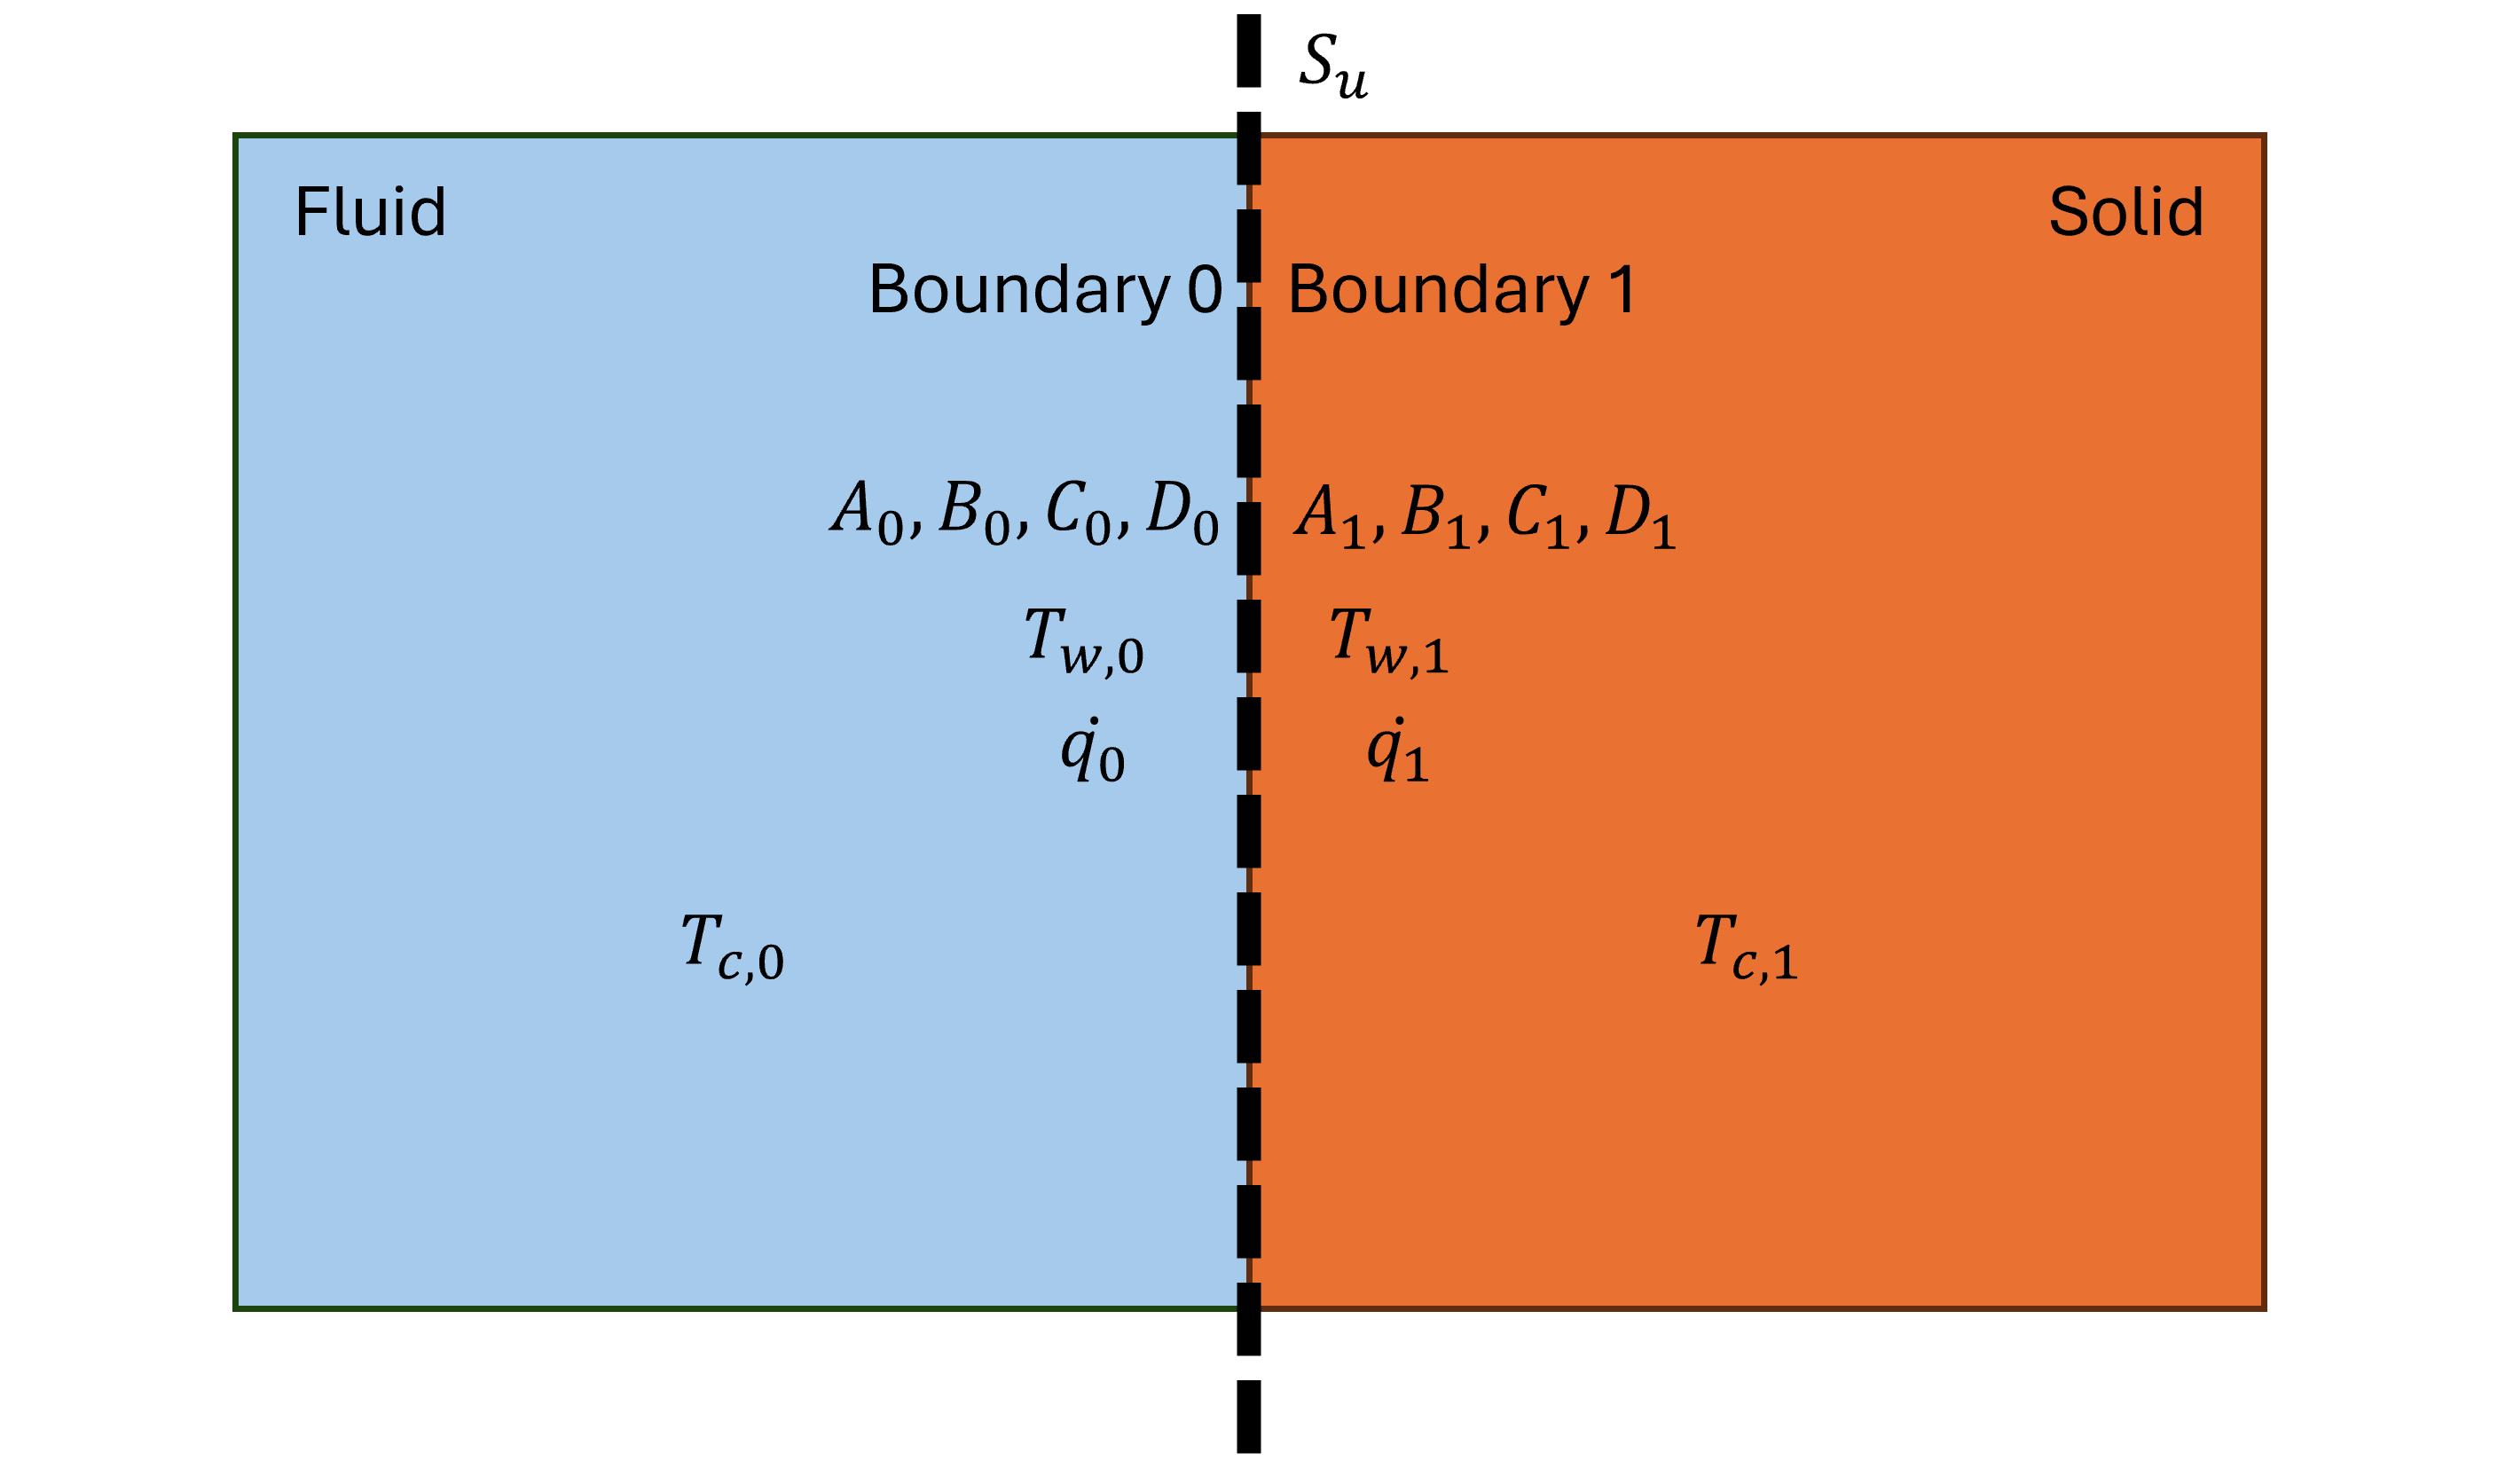
\includegraphics[width=\linewidth]{Figures/conjugateHeatTransferDiagram.png}
\caption{Diagram of the fluid-solid interface at a conjugate heat transfer boundary.}
\label{fig:conjugateHT_diagram}
\end{figure}

The heat flux on each side of the wall is given by

\begin{equation}
    \Dot{q}_{0} = A_{0} + B_{0}T_{c,0} + C_{0}T_{w,0} + D_{0}T^{4}_{w,0},
    \label{eq:q0}
\end{equation}

and 

\begin{equation}
    \Dot{q}_{1} = A_{1} + B_{1}T_{c,1} + C_{1}T_{w,1} + D_{1}T^{4}_{w,1},
    \label{eq:q1}
\end{equation}

where $A$, $B$, $C$, and $D$ are the linearized heat transfer coefficients. These coefficients account for thermal conductivity, convective heat transfer coefficient, and area, and are given by

\begin{equation}
    A = k\left[ \nabla T_{c} - \left( \nabla T_{c} \cdot \mathbf{ds} \right) \vec{\alpha}\right],
    \label{eq:HTC_A}
\end{equation}

\begin{equation}
    B = -k\vec{\alpha},
    \label{eq:HTC_B}
\end{equation}

\begin{equation}
    C = k\vec{\alpha},
    \label{eq:HTC_C}
\end{equation}

and

\begin{equation}
    D = 0. 
    \label{eq:HTC_D}
\end{equation}

With these coefficients, the heat flux across the wall can be obtained with

\begin{equation}
    \dot{q}_0=-\frac{S_u}{2}+\frac{T_{w 1}-T_{w 0}}{R}.
    \label{eq:wallHF}
\end{equation}

\subsection{Solidification Model}
\label{sec:solidmodel}
Solidification is treated in the following way in Star-CCM+'s implementation of the VOF method \cite{starccm}

\begin{equation}
    \alpha^{*}_{s} = \begin{cases}
    1 & T^{*} < 0 \\
    f(T^{*})& 0<T^{*}<1 \\
    0& 1 < T^{*}
    \end{cases},
    \label{eq:solidificationModel}
\end{equation}

\noindent where
\begin{equation}
    T^{*} = \frac{T - T_{solidus}}{T_{liquidus} - T_{solidus}}.
\end{equation}

\noindent latent heat of fusion, $h_{fusion}$ is also taken into account in the model, where

\begin{equation}
    h_{is}^{*} = h_{is} + \left( 1 - \alpha_{s}^{8}\right)h_{fusion}
\end{equation}

\noindent A flow-stop submodel is also employed to stop the fluid flow in the cells that have reached a particular solid threshold (the flowability threshold). In order to maintain numerical stability in the solution of the continuity equation, the density in the stopped cells must be held constant, which is achieved with the flow-stop mass compensation option.  

\subsubsection{Geometry, Mesh, and Boundary Conditions}

In this study, several different microstructures (shown in Fig.~\ref{fig:dimensions}) are evaluated to represent the micro-scale pores. Firstly, a rectangular micro-channel, represented by a two-dimensional (2D) plane extending infinitely into the z-direction. The rectangular channel's purpose is to serve as a benchmark; a case that allows the numerical methods in this model to be compared to analytical models for capillary flow. 

This rectangular geometry was  evaluated against the results from a feathery micro-channel. This feathery micro-channel was scanned by DLR scientists \cite{Sirigiri2018} and a representation of the geometry was converted into a 2D and three-dimensional (3D) geometry, shown in Fig. \ref{fig:dimensions}. The 3D geometry is just the 2D geometry extended into the page. Here, the feathery pattern shown on the right is repeated downward until the TBC column is 200 $\mu m$ deep. This is half the depth of the TBC sample used in experiments \cite{Naraparaju2019}. It should be noted that a typical TBC coating on an aircraft component is $\approx 150 - 180~\mu m$ deep. The TBC coating used in the experiments was larger in order to perform longer kinetic experiments. 

The geometry is then meshed using an unstructured trimmed-cell mesh which can be seen in Fig. \ref{fig:mesh}. The 3D simulations used adaptive mesh-refinement (AMR) at the air-CMAS interface. 

Due to limitations in the 2D model, a separate set of boundary conditions had to be used in the 2D and 3D models. The 2D model is not capable of spontaneously producing capillary flow, unlike the 3D model. The interface resolution, paired with the lack of a inflow/outflow boundary in the z-direction causes the inertial forces to dominate the flow in the 2D model. So, the flow in the 2D model must be ''jump-started`` by an enforced pressure gradient. The boundary conditions for the 2D model are summarized in Table \ref{tab:2DboundaryConditions}. 

Boundary conditions and domain dimensions for the 3D model are summarized in Fig. \ref{fig:dimensions}b and Table \ref{tab:3DboundaryConditions}. Note that only the feathery geometry was simulated in 3D. All flow boundary conditions are zero-gradient, that is, pressure and volume fraction on each of the boundaries is the same as the fluid entering/leaving the boundary. These boundary conditions are important because they ensure the flow of the CMAS is purely driven by capillary effects and not pressure gradients. While it could potentially make more sense to use engine operating pressures for the simulation's reference pressure, this domain was set up to be more in line with experiments conducted by Naraparaju et al. \cite{Naraparaju2014, Naraparaju2017, Naraparaju2019} to ensure the comparison to experimental data is as accurate as possible.

For both the 2D and 3D geometries, conjugate heat transfer was considered by setting the TBC as a solid region, the walls of the TBC were prescribed as a temperature gradient, (i.e. $\Delta T_{x}$), of -1 $K/\mu m$, such that the top of the coating is close to a typical operating temperature for an engine environment. The gradient is defined this way to relate the simulation to the TBC sample that was used in experiments \cite{Naraparaju2019}, which was around 400 $\mu m$ deep, and manages to be around 400 K cooler at the bottom of the TBC than the top, such that the operating temperature is below the melting point of the materials used. It should be noted there is only a gradient in the x-direction, so any walls on the same x-plane will have a constant temperature, and any walls along the same y-plane will have a temperature that varies. 

The wall contact angle of the CMAS phase is expected to be somewhere between 40 and 70 degrees based on experiments \cite{Naraparaju2019}. 
These values are temperature dependent though. For simplicity, a constant wall contact angle of 67 degrees was used \cite{Naraparaju2019}.

The thermal gradient described above for the boundary conditions was also used as the initial temperature condition for both the fluid region and solid region. The fluid domain's initial velocity was set such that there was a very small downward velocity. This is done because it helps with convergence in the first calculations in the simulation.  An additional assumption made in the CFD is that TBC walls are perfectly smooth, which is not necessarily the case in an actual TBC.  Gravity was also enabled to capture any infiltration effects from buoyancy. Turning on gravity also adds the Boussinesq Approximation to the energy equation to account for natural convection. However, the effects of natural convection do not dominate the flow. 


\begin{figure*}
    \centering
    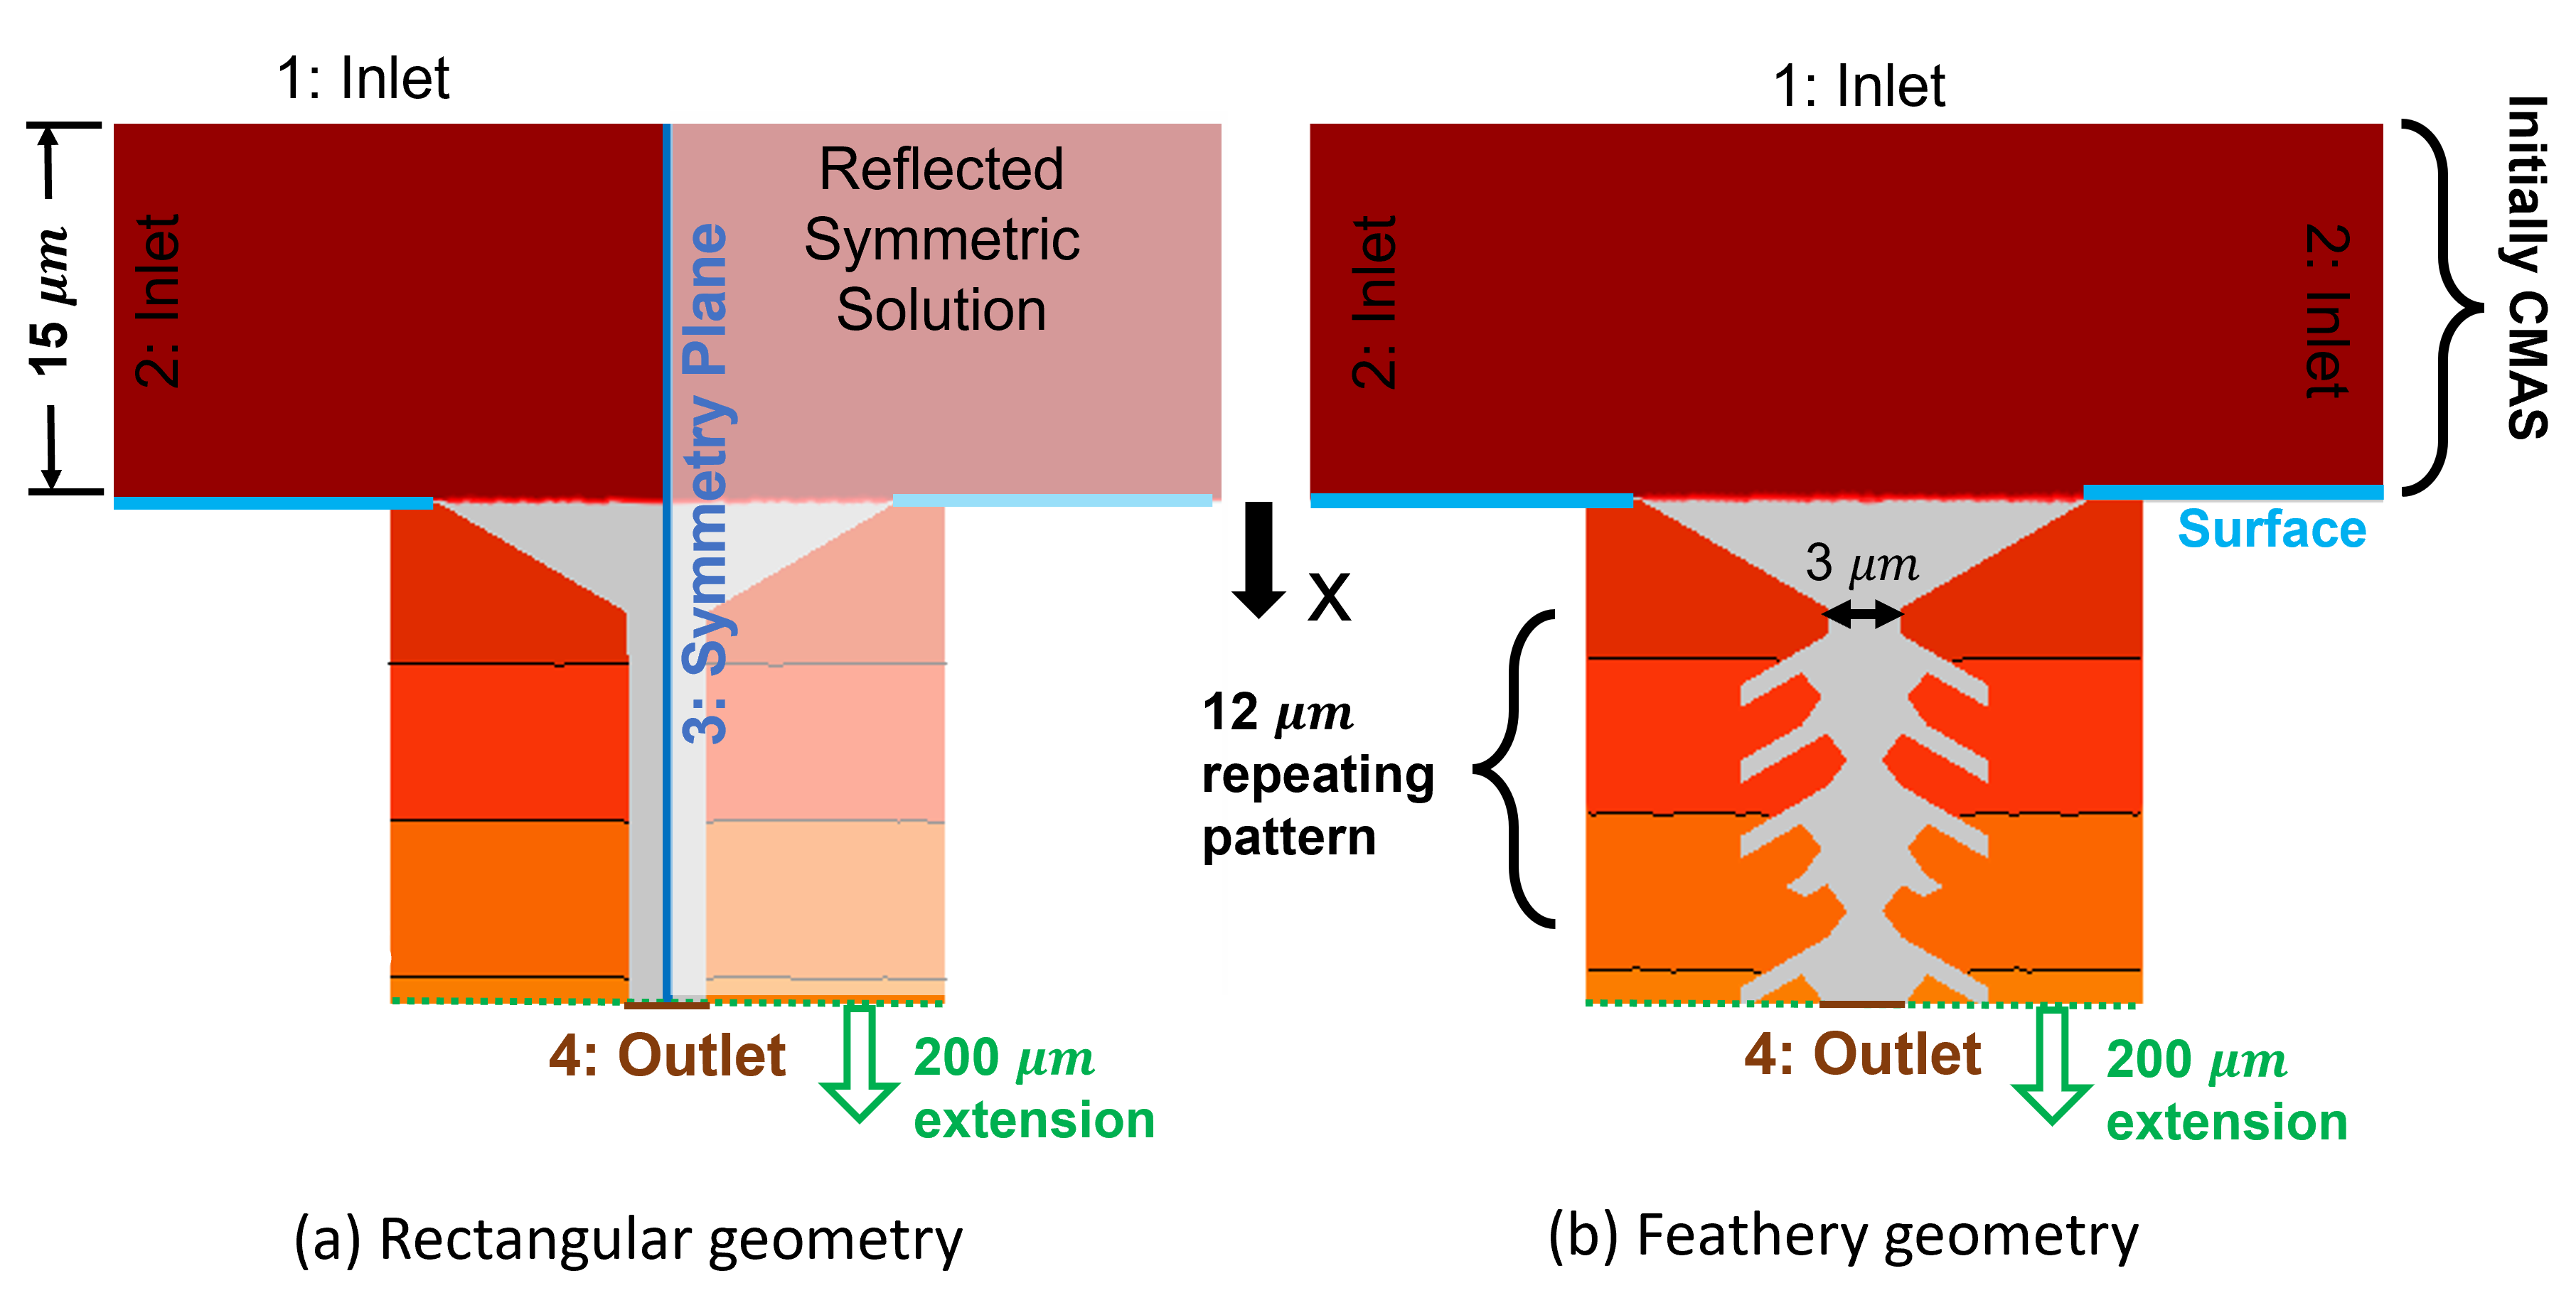
\includegraphics[width=0.9\linewidth]{Figures/dimensionsTwoView.png}
    \caption{Dimensions and boundary conditions applied to two channel types. The contours indicate the thermal boundary conditions in the solid. The dark-red colored area is filled with CMAS which infiltrates into the gray region (air). The red-to-orange gradient represents the decreasing temperature within the TBC as depth increases.}
%    \caption{rectangular (left) and feathery (right) geometries with labeled dimensions and boundary conditions. The dark red colored area shows the starting position of CMAS, and the gray area shows the starting position of air. The red-to-orange gradient represents the decreasing temperature in the TBC as the depth increases.}
    \label{fig:dimensions}
\end{figure*}

% \begin{figure*}
%     \centering
%     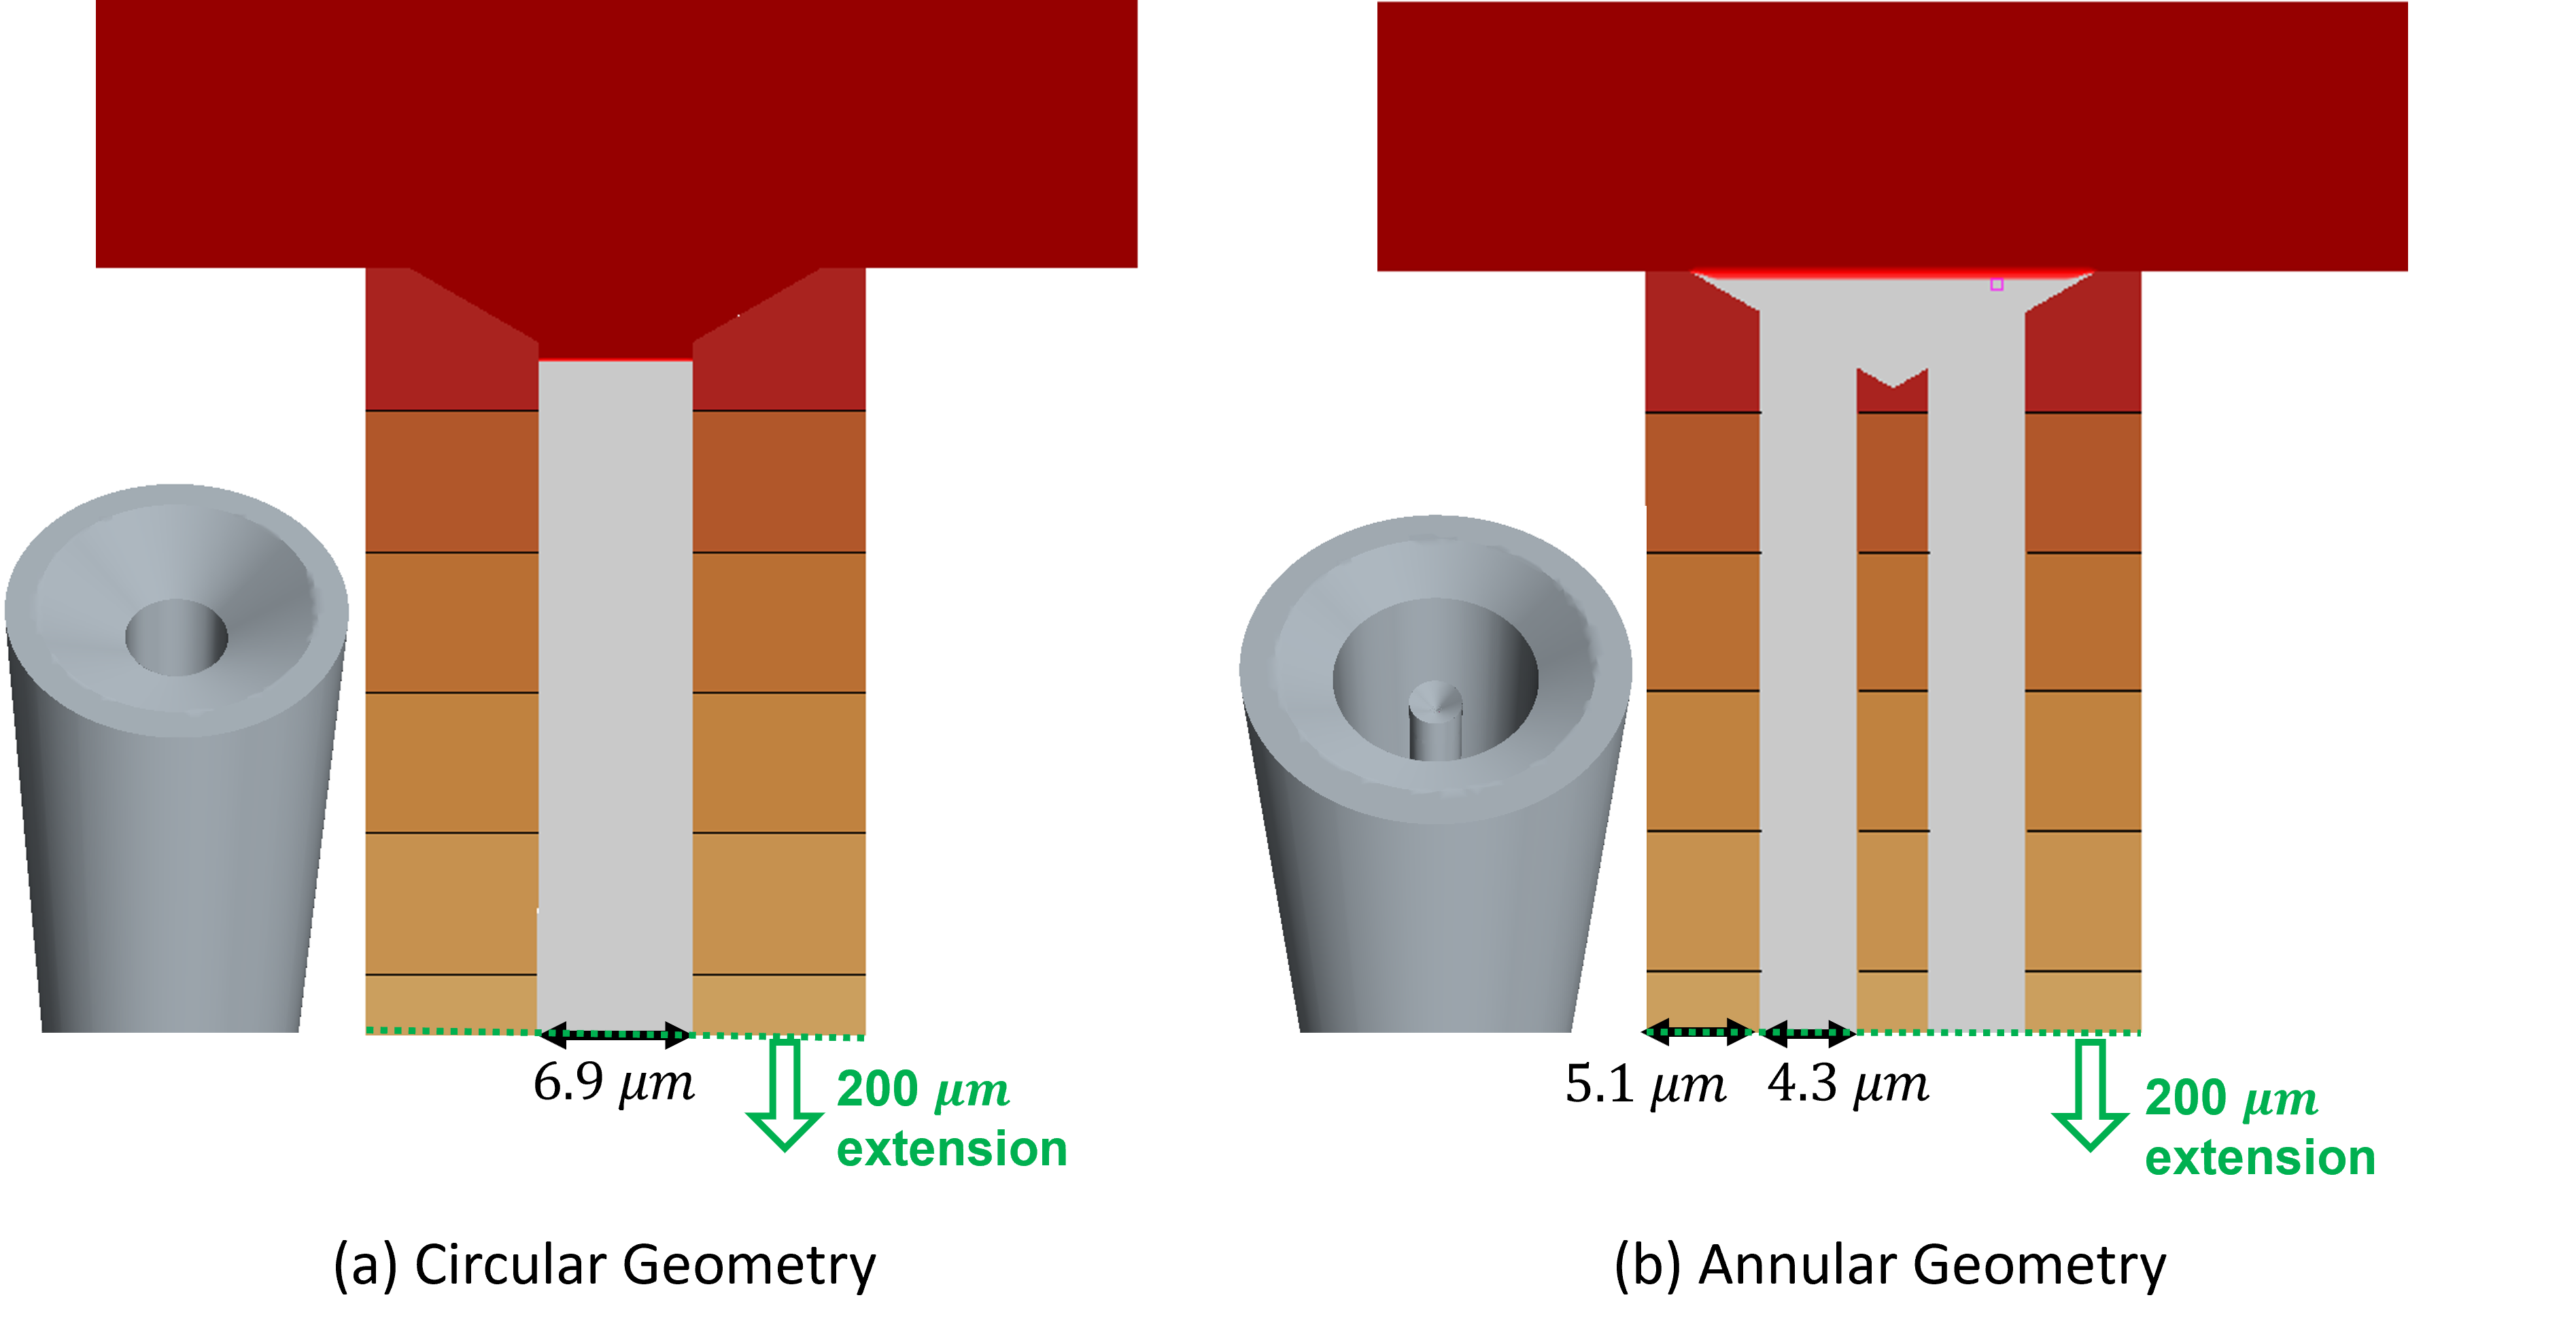
\includegraphics[width=0.9\linewidth]{Figures/3d_geometries.png}
%     \caption{Axisymmetric geometries and dimensions (labeled). Boundary conditions are similar to discussed in Fig.~\ref{fig:dimensions}}
%     \label{fig:3D_Geometries}
% \end{figure*}

\begin{figure}[htp!]
\centering
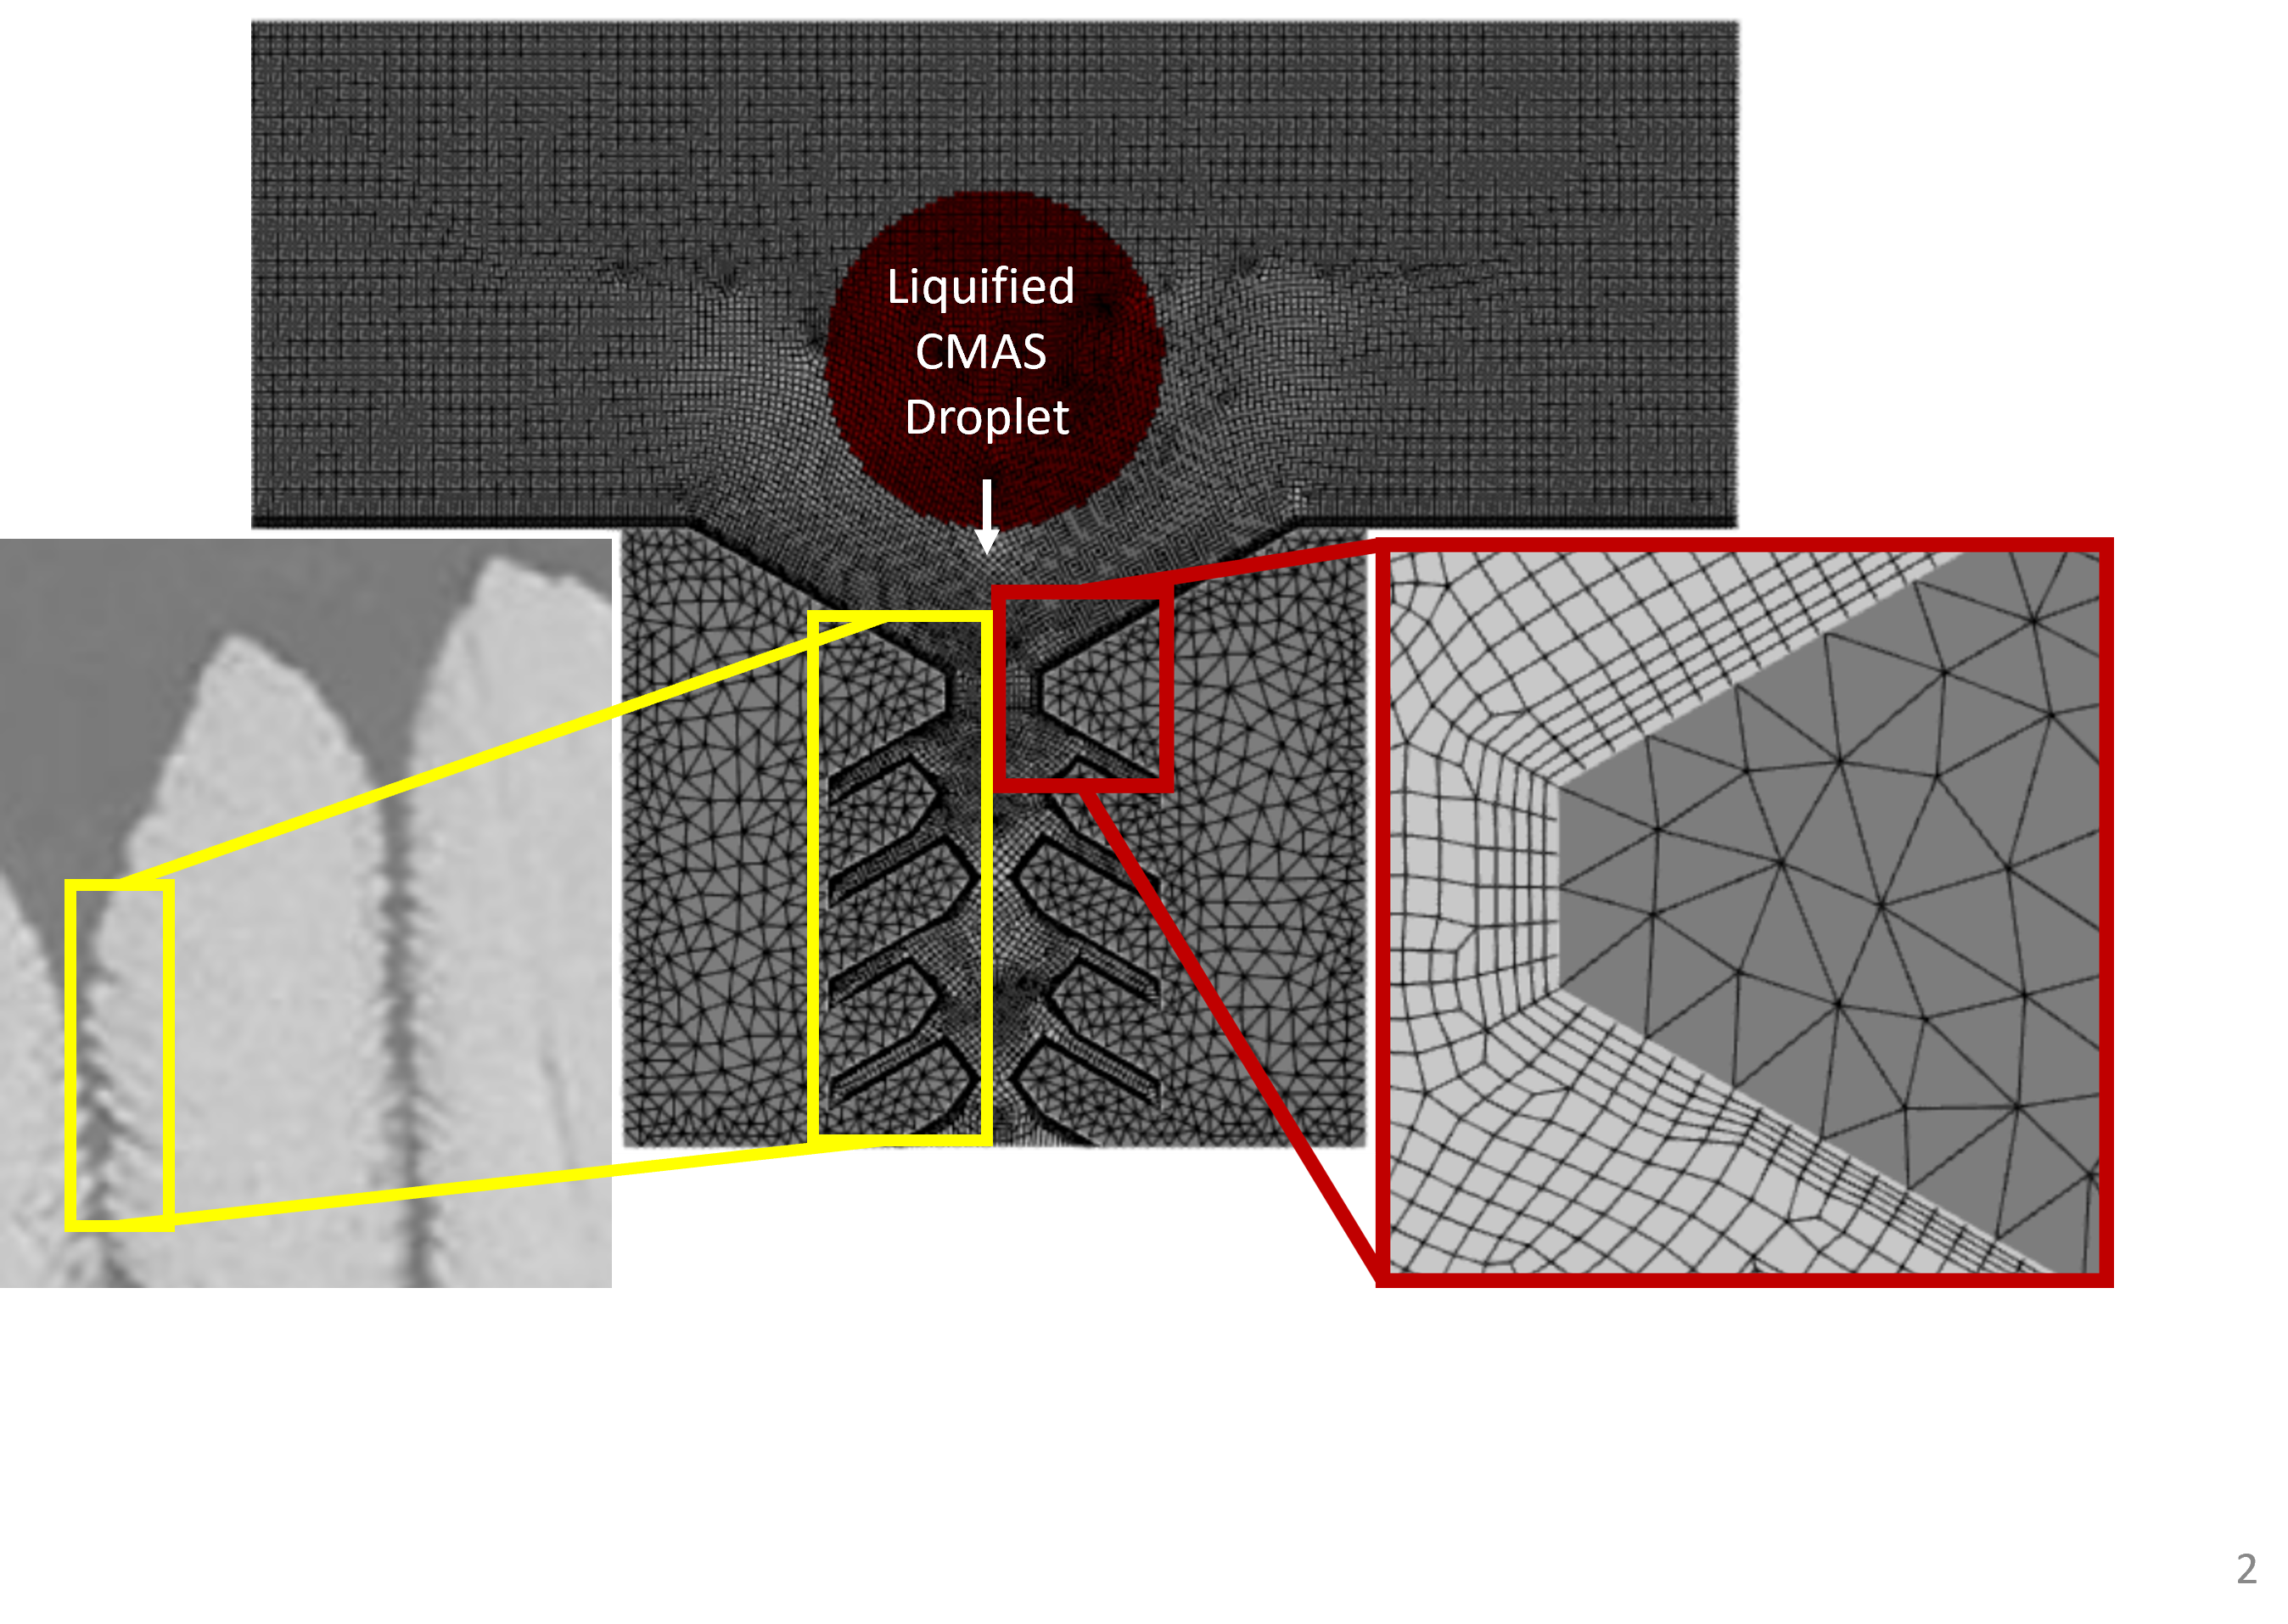
\includegraphics[width=\linewidth]{Figures/mesh_and_sem_compare.png}
\caption{Overall computational mesh and domain compared to a scanning electron microscope (SEM) image (yellow). The mesh has zoomed-in view in the near-wall region. Also, the feather shape can be correlated to feathers from the SEM image.}
\label{fig:mesh}
\end{figure}



\begin{table}[htp!]
\caption{\label{tab:2DboundaryConditions} Summary of labeled boundary conditions for the 2D domain (pressure values with respect to reference pressure $P_{ref} = 101325$ Pa)}
\centering
\begin{tabular}{cccc}
Label &Type& Boundary Condition& Value (Units)\\\hline
1& Inlet&Pressure & 3.0 $MPa$\\
-& -&Temperature& $1530$ K\\
2& Inlet&Pressure& 3.0  $MPa$\\
-& -&$T(x)$& 1530 -$\Delta T_{x}\times x$ (x in $\mu m$)\\
3& Symmetry&- & -\\
4& Outlet&Pressure& -50 $MPa$\\
-& -&Temperature & $1324$ K \\
5& Walls&$T(x)$& 1530 -$\Delta T_{x}\times x$ (x in $\mu m$)\\
\end{tabular}
\end{table}

\begin{table}[htp!]
\caption{\label{tab:3DboundaryConditions} Summary of labeled boundary conditions for the 3D domain (pressure values with respect to reference pressure $P_{ref} = 101325$ Pa). Note that the 3D domain is the same as the 2D domain shown in \ref{fig:dimensions}b, but extended in the -Z and +Z directions (into and out of the page). The -Z and +Z boundary conditions are unlaballed, but are shown in this table.}
\centering
\begin{tabular}{cccc}
Label &Type& Boundary Condition& Value (Units)\\\hline
1& Inflow/Outflow & $\frac{\partial P}{\partial x}$ & 0\\
-& -&Temperature& $1530$ K\\
2& Inflow/Outflow& $\frac{\partial P}{\partial x}$ & 0\\
-& -&$T(x)$& 1530 -$\Delta T_{x}\times x$ (x in $\mu m$)\\
3& Symmetry&- & -\\
4& Inflow/Outflow& $\frac{\partial P}{\partial x}$ & 0\\
-& -&Temperature & $1324$ K \\
5& Walls&$T(x)$& 1530 -$\Delta T_{x}\times x$ (x in $\mu m$)\\
-Z and +Z & Inflow/Outflow& $\frac{\partial P}{\partial x}$ & 0\\

\end{tabular}
\end{table}

%\subsection{Air Phase and Porosity}
Additionally, due to the 2D model assumptions and incompressible air phase, air pockets within the feather gaps demanded paths to escape. To accomplish this, %the interface between the fluid and solid regions 
the fluid-solid interface
was modeled as %set as 
a porous boundary to allow the air to escape. The boundary was modeled with a pressure rise calculated as
\begin{equation}
\label{porous:equation}
    \Delta P = -\rho (\alpha |v_n| + \beta)v_n.
\end{equation}
%The rate at which air was allowed to escape with 
Here, the values of the external pressure ($\Delta P$), inertial resistance ($\alpha$), and viscous resistance ($\beta$), were set to the ambient pressure (i.e., $0 Pa$), 100 (dimensionless), and $1 \frac{m}{s}$, respectively. With this model, the air can escape the pore based on the local pressure and is limited to a maximum velocity of $0.01 \frac{m}{s}$ according to Eq. \ref{porous:equation}.



% \subsection{Modifications to the Governing Equation for Capillary Flow in a rectangular micro-channel}

% For analytical benchmarking, this works seeks to modify an existing governing equations for capillary flow in a micro-channel. One such governing equation for capillary flow in a rectangular micro-channel is given as \cite{Waghmare2012}

% \begin{equation}
%     \left( h^* + C_{1} \right) \frac{d^{2}h*}{dt^{*2}} + C_{2} \left( \frac{dh^{*}}{dt^{*}} \right)^{2}  + \left(C_{3} + C_{4}h^{*} \right) \frac{dh^{*}}{dt^{*}} + C_{5}h^{*} + C_{6} = 0.
%     \label{eq:ODEeq}
% \end{equation}

% \noindent Note that $t^{*}$ and $h^{*}$ are non-dimensional time and depth, and are respectively normalized by $t_{0} =\frac{ \rho 4B^{2} }{12\mu} $ and $ h_{0} = 2B $. The modified coefficients are given and described in Table \ref{tab:ODECoeff}.

% \begingroup
% \setlength{\tabcolsep}{10pt} % Default value: 6pt
% \renewcommand{\arraystretch}{2} % Default value: 1
% \begin{table}[htp!]
% \caption{\label{tab:ODECoeff} Description of Constants and Coefficients in Equation \ref{eq:ODEeq}}
% \centering
% \begin{tabular}{lcccccc}
% \hline
% Coefficient & Definition&\\\hline
% $C_{1}$ & $\frac{0.55}{\alpha_{1}} \sqrt{\gamma}$ \\
% $C_{2}$ & $\frac{\alpha_{1}}{1.158 + \alpha_{1}}$  \\
% $C_{3}$ & $\frac{1}{3\alpha_{1}\left[ \Phi^{4} -6exp\left( \frac{-\Phi^{2}t^{*6}}{3}\right)\right] \times \left[ \Phi^{6} \left( 1-\alpha_{1} \right) - 4\Phi^{2}exp\left( \frac{-\Phi^{2}t^{*6}}{3} + 3\Phi^{4}  \right) \right]}$  \\
% $C_{4}$ &  $\frac{0.295 \sqrt{\gamma}}{\alpha_{1}}$     \\
% $C_{5}$ &  $\frac{Bo}{144\alpha_{1} Oh^{2}}$    \\
% $C_{6}$ &  $\frac{\gamma - cos\theta}{72\alpha_{1} Oh^{2}}$\\
% $\alpha_{1}$ & $\frac{\left[ \Phi^{4} - 4exp\left(- \frac{\Phi^{2}t^{*}}{3}\right) \right]}{\left[ \Phi^{4} - 6exp\left(- \frac{\Phi^{2}t^{*}}{3}\right) \right]}$\\
% $\Phi$ & $\lambda_{n}B$ \\
% $\lambda_{n}$ &$\frac{\left( 2n-1\right)\pi}{2B}$ \\
% \hline
% \end{tabular}
% \end{table}
% \endgroup

% The ODE is solved numerically by converting it from a second-order ODE into a system of first-order ODEs, seen in Equation \ref{eq:linearSystem}. This system is stiff, so it is solved numerically using Matlab's ODE23s algorithm.

% \begin{equation}
% \label{eq:linearSystem}
% \begin{bmatrix}
%     y^{'}_{1} \\
%     y^{'}_{2}
% \end{bmatrix} = 
% \begin{bmatrix}
%     y_{2} \\ 
%     \frac{-C_{2} y_{2}^{2} - (C_{3} + C_{4} y_{1}) y_{2} - C_{5} y_{1} - C_{6}}{y_{1} + C_{1}}
% \end{bmatrix}
% \end{equation}

% Initial conditions from simulations are used to construct a solution to this equation. This solution is compared to simulated, analytical, and experimental results.

\subsection{Previous Theoretical Models: Open-pipe and Concentric-pipe models}
\label{sec:RaviPipeModels}
A summary of the open-pipe and concentric-pipe models is presented here. For a more in-depth description, please see ``Estimation
of CMAS Infiltration Depth in EB-PVD TBCs: A New Constraint Model Supported with Experimental Approach''

\begin{equation}
    t=\frac{\mu r\ h^2}{2\sigma k cos\theta}
    \label{eq:PM_base}
\end{equation}

\noindent here, t is the infiltration time, r is the radius open for infiltration, h is the infiltration depth, $\mu$,$ \sigma$, $\theta$ are viscosity, surface tension, and contact angle respectively \cite{Naraparaju2017,ZHAO201474}. The parameter k represents the porosity and varies depending on whether the open-pipe or concentric-pipe model is being used. Some difficulties arise here, as some of the properties in the above equation vary nonlinearly with temperature, so initial values will be used for the calculations. The open-pipe model defines k as the following

\begin{equation}
    %k_o=\frac{r^2\phi^2}{8\tau\left(1-\phi\right)^2}
    k=\frac{r^2\phi^2}{8\tau\left(1-\phi\right)^2}
    \label{eq:oPM}
\end{equation}

\noindent here $\phi$ is the overall pore fraction, and $\tau$ is a geometric factor based on a ratio of area of the column to area of the feather arms, and it was found to be 2.31 for feathery microstructures \cite{Naraparaju2019}.The concentric-pipe model is similar, but defines k as

\begin{equation}
    %k_o=\frac{\phi}{8\tau^2}b^2\left[1+\frac{a^2}{b^2}+\left(1-\frac{a^2}{b^2}\right)\frac{1}{ln\left(a/b\right)}\right]
    k=\frac{\phi}{8\tau^2}b^2\left[1+\frac{a^2}{b^2}+\left(1-\frac{a^2}{b^2}\right)\frac{1}{ln\left(a/b\right)}\right]
    \label{eq:CPM}
\end{equation}

\noindent where a and b are the outer radii of the concentric pipes \cite{Naraparaju2019}. 


\subsection{Theoretical Model: FPNM}
\label{sec:pipeNetworkMethod}
This works also seeks a more representative, but still intuitive way of describing the flow within the feathery microstructure of a TBC. Therefore, a feathery-pipe-network model (FPNM)  is formulated and proposed and is based on considering a network of capillary channels. This model was inspired by a capillary flow electrical circuit analogy \cite{Mikaelian2020}. However, the circuit analogy does not allow for configurations matching the TBC gap. So, FPNM is proposed. Theoretical model development has also shown that the Lucas-Washburn equation can indeed be extended into larger, heterogeneous porous media \cite{Cai2021, WAGHMARE2010561}, but this theoretical model is also more generalized and is difficult to specifically model the configurations seen in Figure \ref{fig:dimensions}.
In FPNM, there is a primary channel, with other secondary channels extending (almost) perpendicular from the primary tube. In the context of the FPNM, these secondary channels, effectively retard the primary-channel flow. The FPNM model formulation demands added input using the following variables (which can be referenced in Fig. \ref{fig:FPNM_cartoon}:

\begin{itemize}
    \item $n$, the number of secondary channels affecting the flow in the primary channel (increases as depth of CMAS in primary tube increases)
    \item $h_{p}$, the depth of the CMAS in the primary channel
    \item $h_{s}$, the depth of the CMAS in a secondary channel
    \item $B$ is the inter-columnar gap (width of the primary channel)
    \item $b$ is the feather gap width
    \item $\Delta b$ is the separation between each feather gap
    \item $\theta$ is the feather angle
    \item $L_{s}$ and $L_{p}$ are the lengths of the primary channel (the coating depth), and the feather length respectively
\end{itemize}

\begin{figure}
    \centering
    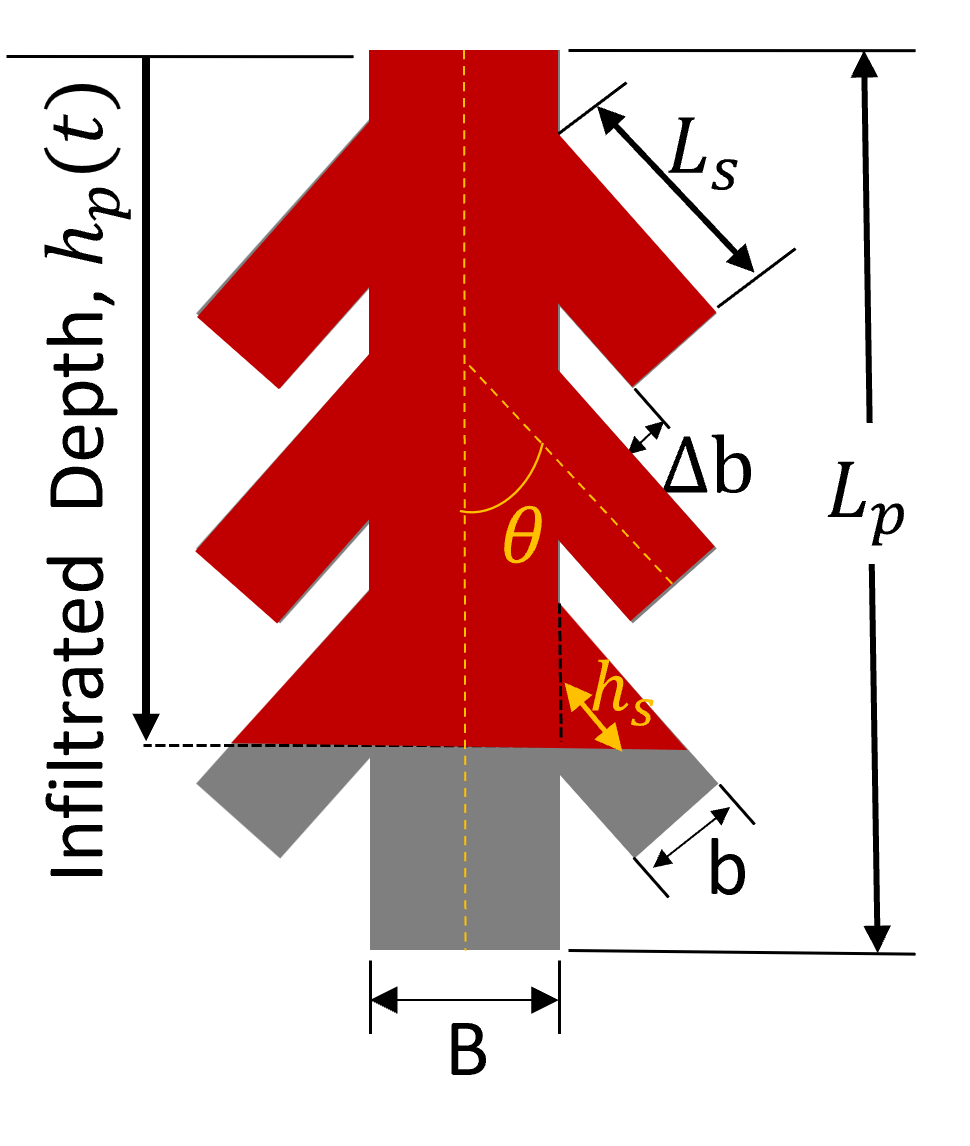
\includegraphics[width=\linewidth]{Figures/FPNM_cartoon.png}
    \caption{Visual representation of geometric parameters describing FPNM}
    \label{fig:FPNM_cartoon}
\end{figure}

\noindent A visual representation of these variables is shown in Fig.~\ref{fig:FPNM_cartoon}. It is proposed to adapt these variables into the Washburn model\cite{Washburn19213}, which is given as

\begin{equation}
    \frac{dh}{dt} = \frac{d^{2}}{\mu}\frac{\Delta P}{L}.
\end{equation}

\noindent Where $\Delta P = \sigma/d$, this is the proposed relation for the primary channel, as so

\begin{equation}
    \frac{dh_{p}}{dt} = \frac{B^{2}}{\mu}\frac{\Delta P}{L_{p}}.
\end{equation}

\noindent However, an additional term to account for the flow in the secondary channels must be added (i.e. the flow that is causing ``resistance'' in the primary channel). If we assume that this resistance, $R_{s}$, takes the form

\begin{equation}
    R_{s} = \frac{b^{2}}{\mu}\frac{\Delta P}{L_{s}}cos\theta,
\end{equation}

\noindent it can be said that 
\begin{equation}
        \frac{dh_{p}}{dt} = \frac{B^{2}}{\mu}\frac{\Delta P}{L_{p}} -ncos\theta\frac{b^{2}}{\mu}\frac{\Delta P}{L_{s}}.
\end{equation}

\noindent The number of feathers affecting the flow in the primary channel ($n$) increases as the depth of CMAS in the primary channel increases. However, $n$ can be solved directly since the primary channel height ($h_p$), feather width ($b$), and feather gap width ($\Delta b$) are known.

\begin{equation}
    n = 2\frac{h_{p}}{b + \Delta b}.
\end{equation}

\noindent So the overall equation becomes, after substituting $\Delta P = \sigma/d$,

\begin{equation}
    \frac{dh_{p}}{dt} = \frac{B \sigma}{h_{p}\mu} - 2 cos\theta\left(\frac{h_{p}}{b + \Delta b} \right)\frac{b \sigma}{L_{s}\mu}.
\end{equation}


\noindent Now, it is assumed that the time it takes for the flow to infiltrate the feathers, $L_{s}(t)$ is much smaller than the time scale of the primary flow. So, $L_{s}(t)$ can be integrated with respect to time to get 
\begin{equation}
    L_{s}\left( t \right) = \sqrt{\frac{\sigma t b}{\mu}}.
\end{equation}

\noindent Implementing this definition and rearranging yields a time-dependent differential equation

\begin{equation}
    \frac{dh_{p}}{dt} = \frac{\sigma B}{\mu} \frac{1}{h_{p}(t)} - 2 cos\theta h_{p}(t) \left( \frac{1}{b+\Delta b} \right) \sqrt{\frac{\sigma b}{\mu t}}
    \label{eq:FPNM_dimensional}
\end{equation}

\noindent which can be rearranged and rewritten in terms of the $Oh$ with respect to the primary channel, as well as non-dimensional variables $h_p^* = h_p/B$, and $t^* = t/t_{B}$, where $t_{B} = \sqrt{\frac{\rho B^{3}}{\sigma}}$
\begin{eqnarray}
\label{eq:FPNM_non-dimensional}
    &&h_{p}^{*}\left(t^{*}\right)\frac{dh_{p}^{*}}{dt^{*}} + 2 cos\theta \sqrt{\frac{\rho B^{3}}{\sigma}} \left( \frac{1}{b+\Delta b} \right)\left(h_{p}^{*}\left(t^{*}\right)\right)^{2} \\
    && + \sqrt{\frac{\sigma b}{\mu B^{2}}} \frac{1}{\sqrt{t^{*}}} h_{p}^{*} \left(t^{*}\right) = Oh_{B}^{-1}. \nonumber
\end{eqnarray}
% \begin{equation}

% \end{equation}


\noindent Here, we have a nonlinear, first-order ODE that is readily solvable. To account for non-linear variations of fluid properties, such as viscosity, Eq.~\ref{eq:FPNM_non-dimensional} is solved in small time increments, and the properties are updated after each increment. Importantly, the maximum viscosity is limited to the viscosity the CMAS achieves at its solidification temperature. Viscosity does not change above this point in FPNM.

\chapter{RESULTS AND DISCUSSION}
\section{Shock-droplet Interactions}
\label{sec:shockDropResults}

This section will outline the preliminary results from each method described in Section \ref{sec:shock-droplet_method}, and discuss what further work is necessary in order to formulate a coherent journal article.

The shock-droplet interaction CFD simulation was carried out for various $M_{shock}$ such that $We_{droplet}$ was varied throughout the various breakup regimes \cite{PILCH1987741}. 
In the following sections, we assess the effect of $M_{shock}$, $We_{droplet}$, and cavitation on the droplet shape, driving forces of breakup, and secondary droplet distribution.



\subsection{Driving Forces of Droplet Deformation and Breakup}

Now, we examine how the passive scalars described for force accumulation (Equations~\ref{eq:pressureIntegrated} and ~\ref{eq:shearIntegrated}) behave.
The goal is to understand the fundamental driving forces of droplet breakup, and to identify forces in regions of interest (such as regions likely to cavitate.)
This is accomplished, first, by qualitatively visualizing the passive scalars in the droplet after the shock has passed over it, seen in Figure~\ref{fig:shear_pressure_accumulation}.
Now, we highlight information that can be inferred from Figure~\ref{fig:shear_pressure_accumulation}.\\

The accumulated shear stress in Figure~\ref{fig:shear_pressure_accumulation} is distributed along the air-water interface.
Along this interface, at $\approx 45 \degree$ from the horizontal axis, the accumulated shear switches from negative to positive. This area is highlighted in Figure~\ref{fig:roll_up_points}
Hence, the point at which the switch occurs is experiencing tension; the interfacial cells adjacent to this cell are being pulled in opposite directions.
This provides evidence that this point is where initial droplet roll-up is experienced.
Interestingly, a Kelvin-Helmholtz (K-H) instability also arises at this point.
This finding somewhat contradicts findings that say the ``pit''  at this particular location is formed because of the interaction with the triple-point of the shock \cite{Xu2024}.
The planar shock structure being used for this study does not have a triple-point, unlike Xu's cellular detonation wave. So, in the present case, the surface instability must be responsible for the pit formation.


\begin{figure}
    \centering
    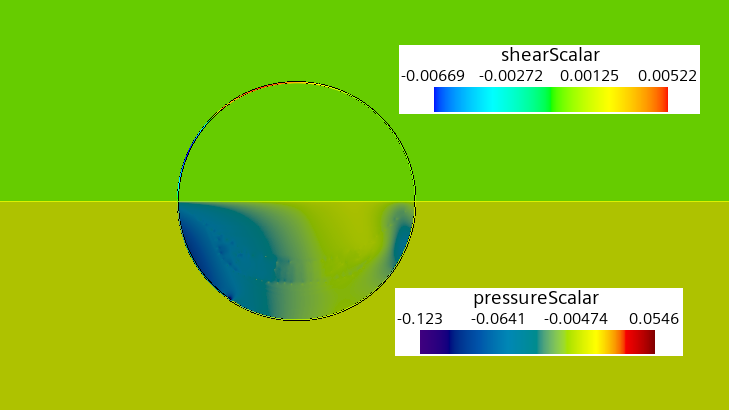
\includegraphics[width=0.8\textwidth]{Figures/pressure_and_shear_accumulation.png}
    \caption{Accumulation of shear stress and pressure on the droplet after the shock has passed over the droplet. The shear stress accumulates along the air-water interface whereas the pressure accumulates both on the interface and within the droplet.}
    \label{fig:shear_pressure_accumulation}
\end{figure}

\begin{figure}
    \centering
    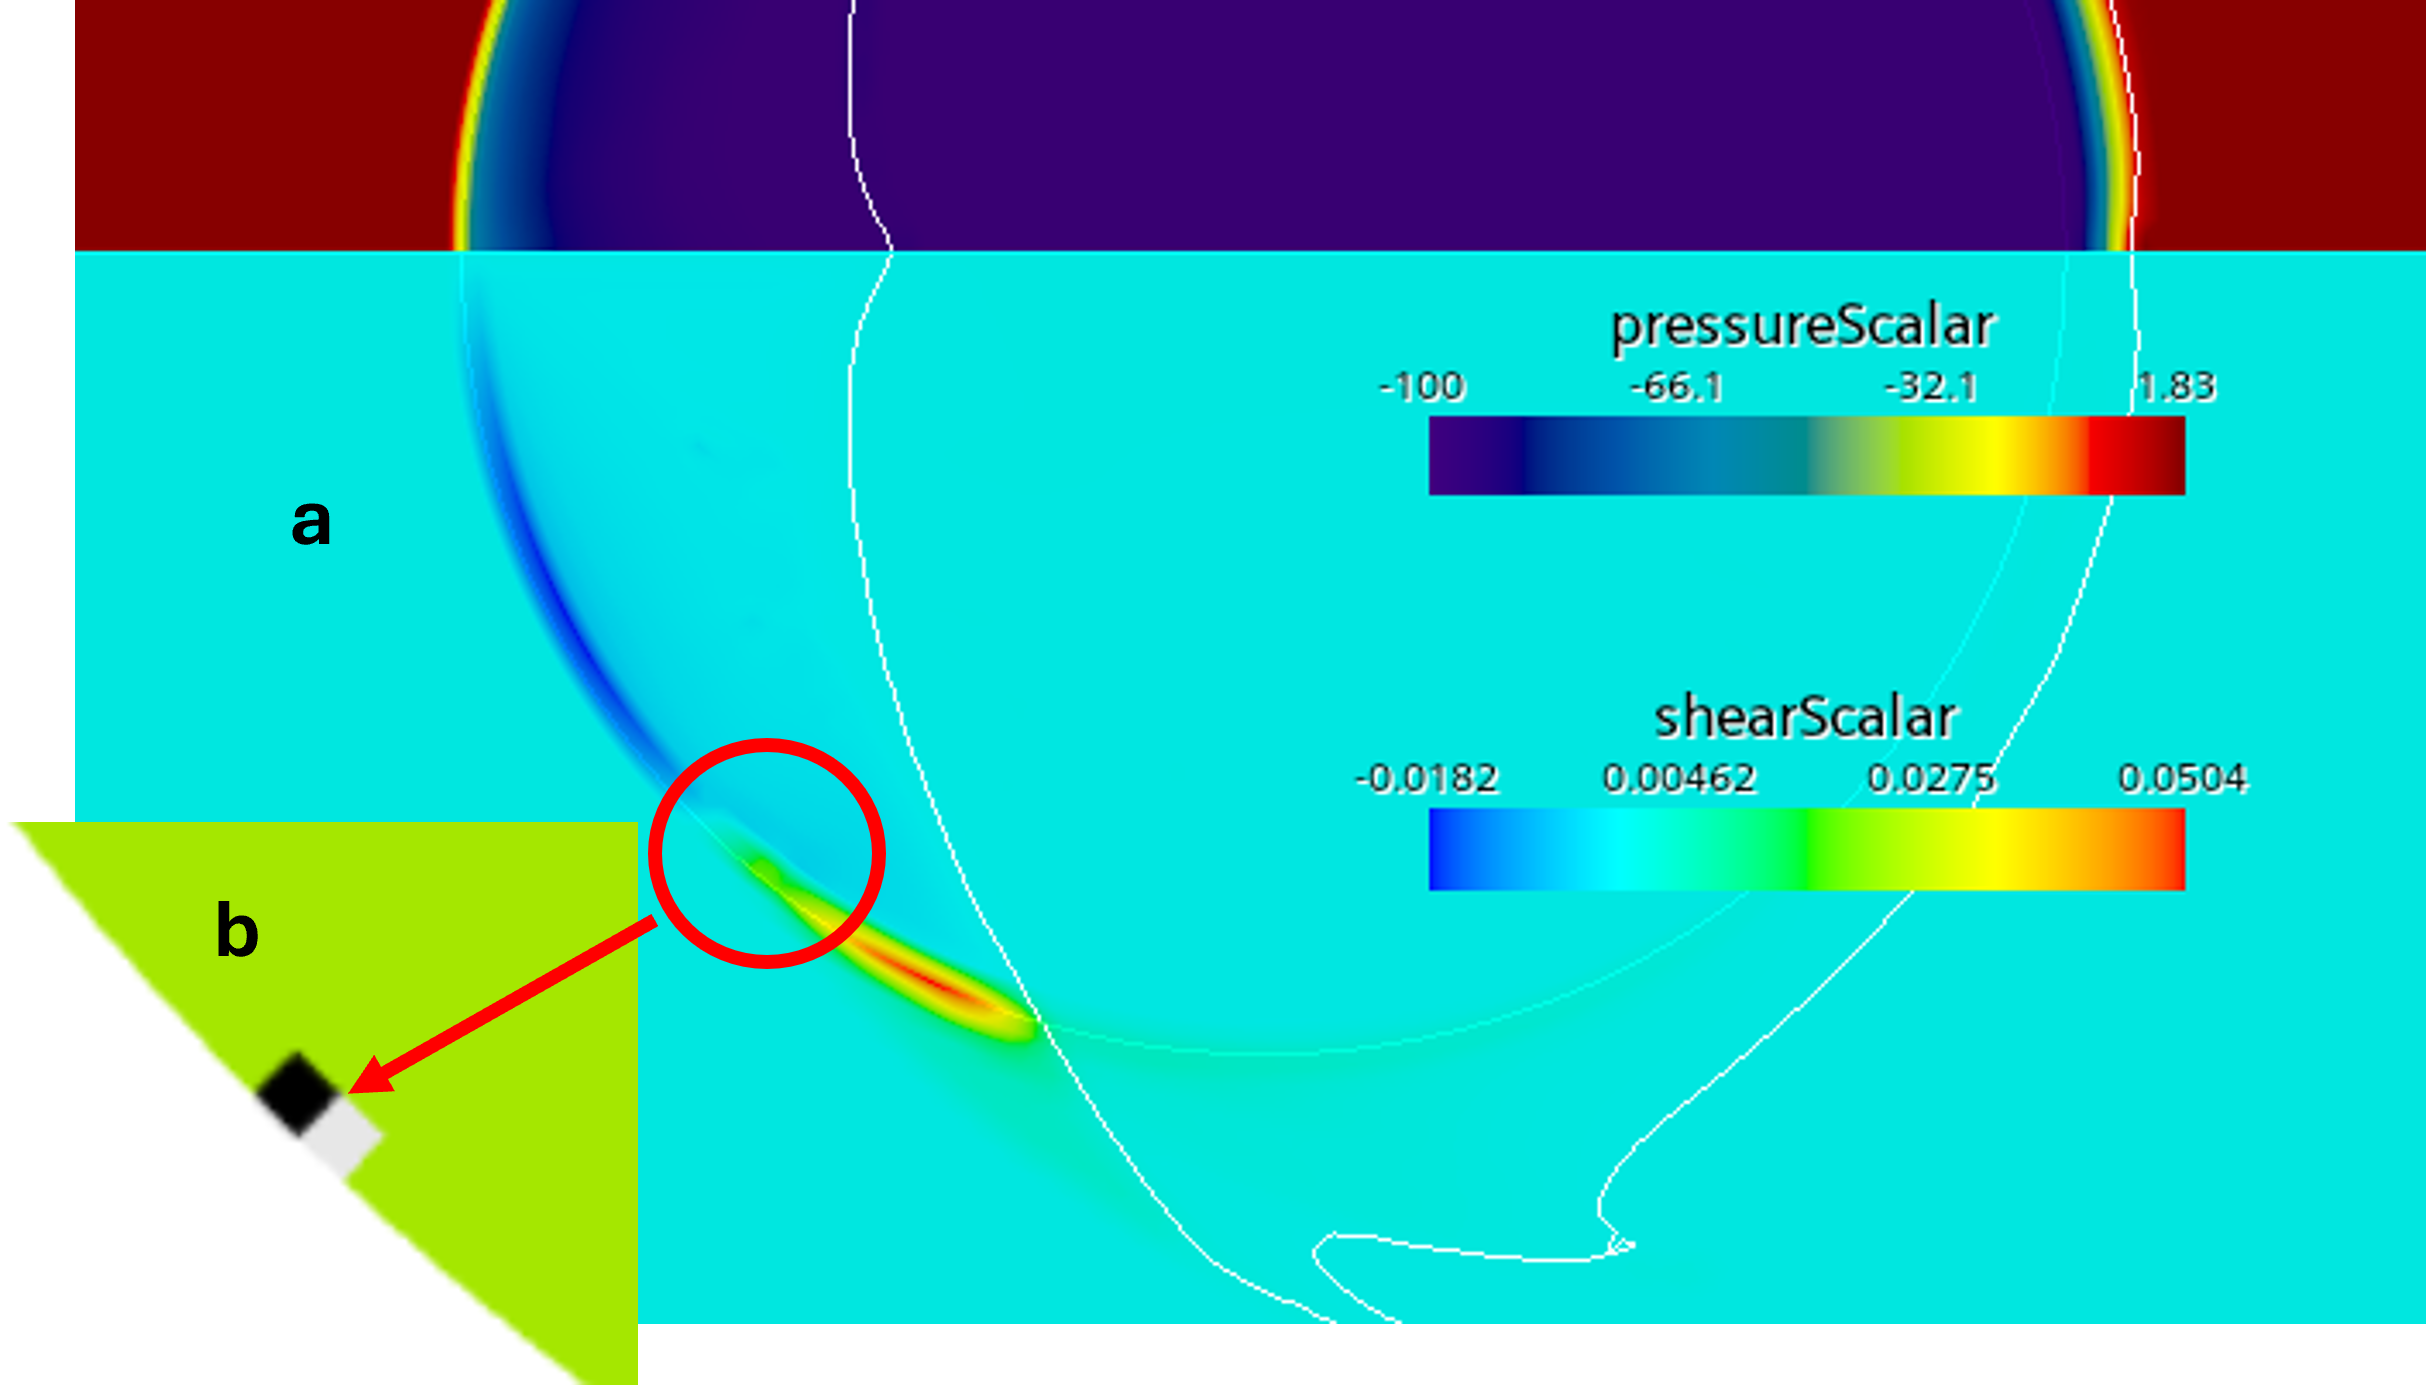
\includegraphics[width=0.8\textwidth]{Figures/roll_up_points.png}
    \caption{(a) Zooming in on the shear stress accumulation in the droplet to see the point at which shear stress switches from positive to negative. (b) Zoomed-in image of the roll-up point, where a mask has been applied to the accumulated shear stress to separate positive and negative shear stress. This elucidates the exact cells that correlate to the roll-up point.}
    \label{fig:roll_up_points}
\end{figure}

Now, this begs the question \textit{does Mach No. affect where this initial roll-up occurs?} To answer this question, this methodology was carried out for droplets at various $M_{shock}$, and the location of the roll-up point was tracked. The results from this can be seen in \ref{fig:roll_up_points_data}.
Here, the roll-up point location was tracked in degrees relative to the droplet center, starting from 0\degree at the leading edge of the droplet

\begin{figure}
    \centering
    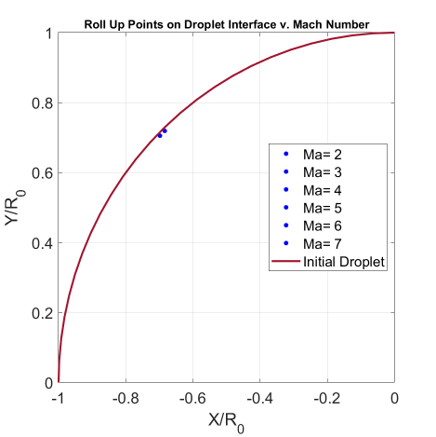
\includegraphics[width=0.8\textwidth]{Figures/roll_up_Mach.png}
    \caption{Location of the initial roll-up point (the point where the Kelvin-Helmholtz instability initiates) as a function of Mach Number. Here, it is shown that the location of the roll-up point is largely independent of Mach Number.}
    \label{fig:roll_up_points_data}
\end{figure}

Another way to understand how droplet deformation can occur is to observe the boundary layer along the droplet's surface.
Figure \ref{fig:boundary_layer_v_Mach} shows how the droplet's boundary layer changes with respect to $M_{shock}$ at different non-dimensional times ($t^{*} = \frac{t-t_{impact}}{D \times c_{H2O}}$). Figure \ref{fig:BL_diagram} shows where the velocity information was extracted for these boundary layers.
The boundary layer is directly related to the shear stress the droplet is experiencing along the interface. 
This is a result of Newton's Law of Viscosity, where $\tau_{w} = \mu \left[\frac{\partial u}{\partial y}\right]_{y=0}$. 
From this, there are many ways to estimate skin friction and pressure drag given the boundary layer information. 

\begin{figure}
    \centering
    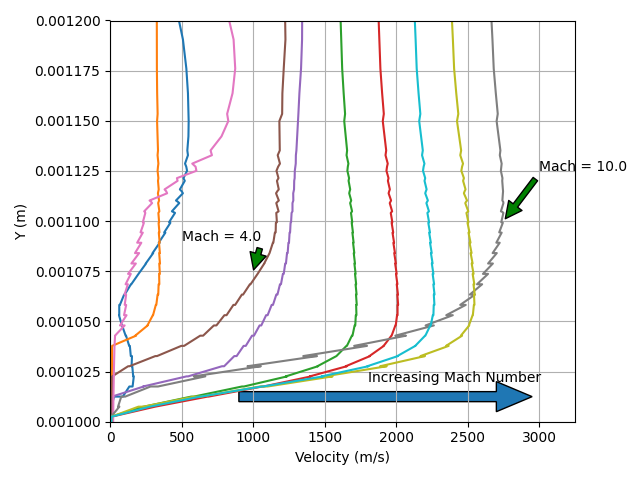
\includegraphics[width=0.8\textwidth]{Figures/coplotted_BLs.png}
    \caption{Droplet's velocity boundary layer for $M_{shock} = 1.0, 2.0,...,10.0$ taken at the location marked in Figure \ref{fig:BL_diagram}. From left to right, top to bottom, $t^{*} = \frac{t-t_{impact}}{D \times c_{H2O}} = 1.0, 2.0, 3.0, 4.0$.}
    \label{fig:boundary_layer_v_Mach}
\end{figure}

\begin{figure}
    \centering
    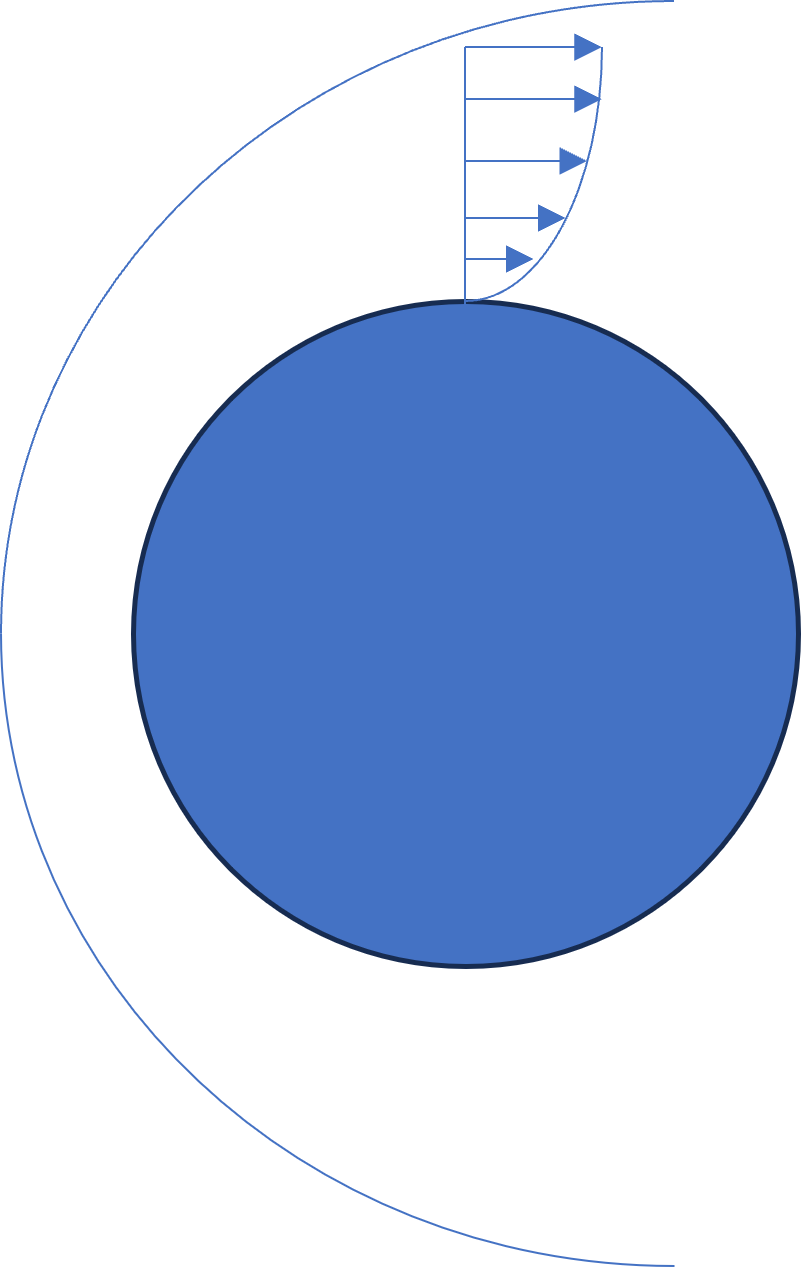
\includegraphics[width=0.25\textwidth]{Figures/BL_diagram.png}
    \caption{Diagram of the boundary layer surrounding the droplet, where the boundary layer height is governed by the post-shock velocity.}
    \label{fig:BL_diagram}
\end{figure}

Figure \ref{fig:boundary_layer_v_Mach} shows that the boundary layers all have a similar shape, and the height of the boundary can be approximated by the location of the maximum velocity in the boundary layer. The maximum velocity is of a similar magnitude as the post-shock velocity once the bow shock has formed around the droplet.
Once the boundary layer height is calculated, boundary layer theory can be used to determine the skin friction drag coefficient, $C_{f} = \frac{\tau_{w}}{0.5 \rho U^{2}_{post-shock}}$.

\begin{figure}
    \centering
    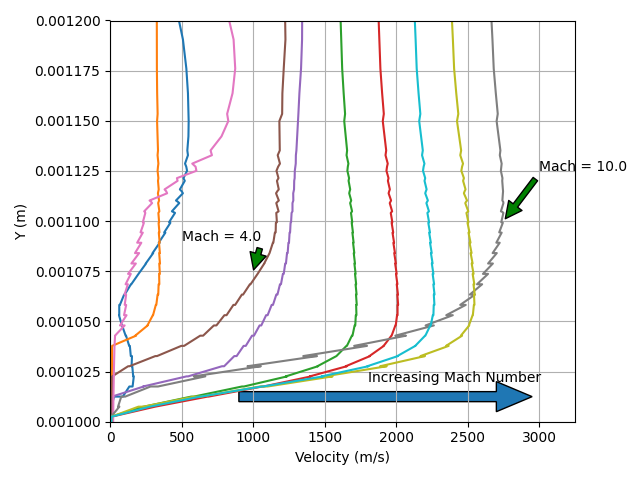
\includegraphics[width=0.8\textwidth]{Figures/coplotted_BLs.png}
    \caption{Droplet's velocity boundary layer for $M_{shock} = 1.0, 2.0,...,10.0$ taken at the location marked in Figure \ref{fig:BL_diagram}.}
    \label{fig:BL_heigh_v_mach}
\end{figure}

Using Newton's Law of Viscosity, $\tau_{w}$ can be approximated by replacing the velocity derivative with a finite-difference near the interface.
This is done for every cell along the interface before the flow detaches from the droplet ($\theta \approx 150\degree$). Shear force is in the detached region is negligible \cite{Khan2004}. 
Now, $\tau_{w}$ is multiplied by $2\pi$ to convert to an axisymmetric value to a full 3D value. \\
It may also be possible to estimated the skin friction drag only knowing the boundary layer height.


\subsection{Results of One-way Coupled CFD/Cavitation}

\subsubsection{Evaluating $T$ and $\Bar{p}$}

Now we evaluate areas within the droplet where absolute pressure is less than vapor pressure for a significant amount of time.
$\Bar{p}$ and $T$ are evaluated in these areas to determine potential for bubble growth and cavitation.
Figure~\ref{fig:underpressure_cav_time} shows $T$ and $\Bar{p}$ within the droplet as the simulation progresses. 
After the initial wave enters and propagates through the droplet (Figure~\ref{subfig:initialWave}), the point at which the wave is focused experiences a significant drop in pressure, and thus, has the most potential cavitation time.
This time period will be referred to as $T_{1}$ henceforth. \\

Figure~\ref{subfig:first_reflection} shows the droplet after the wave has reflected off the trailing edge of the droplet and reached the leading edge. 
The reflection causes the first underpressure region to grow, causing more energy to be available for cavitation than the initial propagation alone.
A new region of the droplet toward the leading edge also enters the cavitation regime.

The pattern above tends to repeat; existing regions of potential cavitation grow in size and magnitude, and new regions enter the cavitation regime.
This happens until the reflecting wave is no longer strong enough to decrease the absolute pressure below the vapor pressure.
While some regions are in the cavitation regime for longer periods of time, others have increased $\Bar{p}$.
This emphasizes how the likelihood of cavitation is not just dependent on the time in tension, but the strength of the tensile force as well.\\

Figure~\ref{fig:cav_time_and_underpressure_centerline} shows the total time spent under vapor pressure and the integral with respect to time of the pressure when it is under vapor pressure.
The data in this figure further highlights that there are two components of potential cavitation: time, and magnitude.
Figure~\ref{fig:cav_time_and_underpressure_centerline} (top) shows that the point along the droplet centerline that is under vapor pressure for the most time is close to the droplet center.
However, Figure~\ref{fig:cav_time_and_underpressure_centerline} (bottom) shows that the point which experiences the largest magnitude of underpressure is toward the trailing edge of the droplet.


\begin{figure}
    \centering
    \begin{subfigure}[b]{0.3\textwidth}
        \centering
        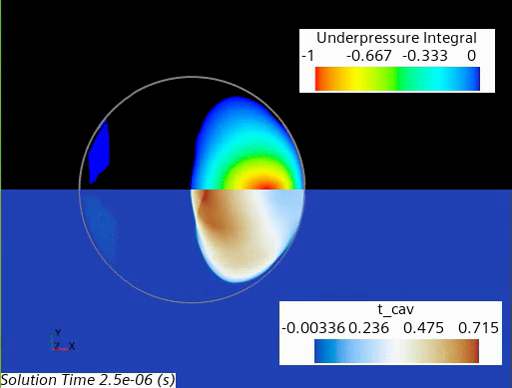
\includegraphics[width=\textwidth]{Figures/init_shock.png}
        \caption{$\phi_{\Bar{p}}$ and $T$ at $T_{1}$}
        \label{subfig:initialWave}
    \end{subfigure}
    \begin{subfigure}[b]{0.3\textwidth}
        \centering
        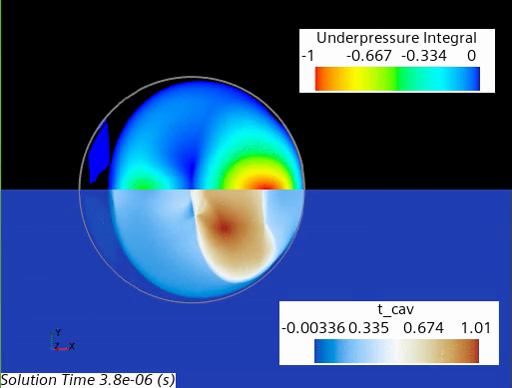
\includegraphics[width=\textwidth]{Figures/reflect_1.png}
        \caption{$\phi_{\Bar{p}}$ and $T$ at $T_{2}$}
        \label{subfig:first_reflection}
    \end{subfigure}
    \begin{subfigure}[b]{0.3\textwidth}
        \centering
        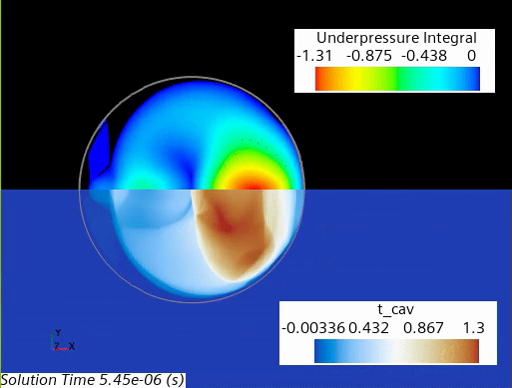
\includegraphics[width=\textwidth]{Figures/reflect_n.png}
        \caption{$\phi_{\Bar{p}}$ and $T$ at $T_{n}$}
        \label{subfig:n_reflections}
    \end{subfigure}
    \caption{Evolution of $\phi_{\Bar{p}}$ (top) and $T$ (bottom) through time. In \ref{subfig:initialWave}, a region toward the trailing edge of the droplet enters the underpressure regime, concentrated where the shockwave was focusing via lensing. In \ref{subfig:first_reflection}, the pressure wave reflects off of the trailing edge and moves back to the leading edge, and is focused toward another point that enters the underpressure regime. ~\ref{subfig:n_reflections} shows that this pattern continues, increasing the magnitude of $T_{max}$ and $|\phi_{\Bar{p}}|$ in regions that have already entered the underpressure regime, and causing new regioons to under the regime as well.}
\label{fig:underpressure_cav_time}
\end{figure}

\begin{figure}
    \centering
    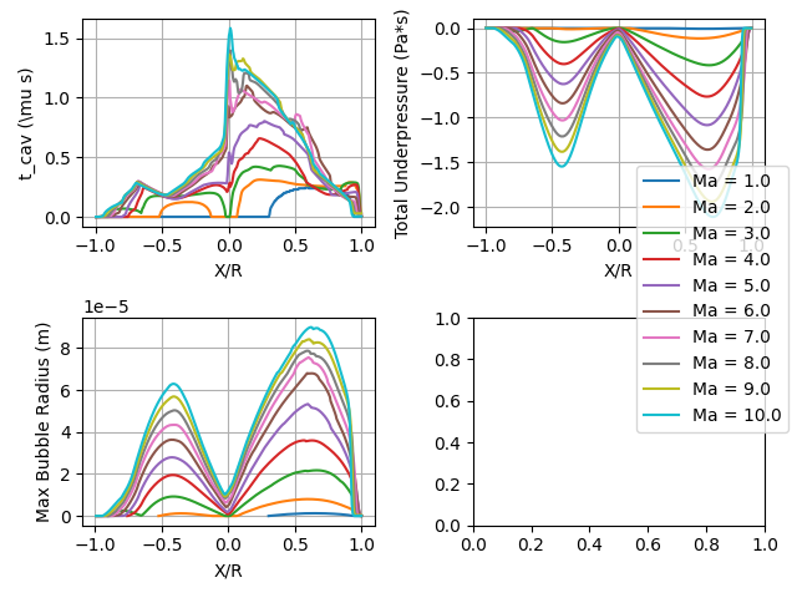
\includegraphics[width=0.9\linewidth]{Figures/cavitation.png}
    \caption{Variation of cavitation time (top) in $\mu s$ and total underpressure (bottom) in Pa along the center axis of the droplet. The data was extracted at 14.3 $\mu s$. Here, it is shown that increasing $Ma$ decreases the total time spent under vapor pressure, and the amount by which the pressure drops. This suggests $Ma$ and cavitation potential have an inverse relationship beyond the $Ma$}
    \label{fig:cav_time_and_underpressure_centerline}
\end{figure}

Figure~\ref{fig:pressure_mach_sweep} shows the time history of pressure at the points highlighted in Figure \ref{fig:point_probes}.
Here, it is easy to see how the intensity of the pressure spikes increase with $Ma$.
The absolute pressure within the droplet also increases with $Ma$.
This happens because as the bow shock forms around the droplet, the droplet essentially becomes pressurized as it is surrounded by high-speed air.
Interestingly, this effect subsides as the measurement location moves from P0 to P9.
Interestingly, as the pressure is measured closer to the droplet center, the spacing between pressure spike events becomes more uniform.
The negative pressure spikes are also less intense toward the droplet center.
This indicates that cavitation is less likely to occur at the droplet center, a finding that is supported by the time-integrated underpressure in \ref{fig:cav_time_and_underpressure_centerline} as well.\\

In the front half of the droplet, the negative pressure spikes tend to be less intense than the positive pressure spikes.
However, in the back half of the droplet, the negative pressure spikes are more intense than the positive pressure spikes.
This supports the idea that the region of the droplet closest to the trailing edge is more likely to cavitate. This finding is again supported by the total time spent under vapor pressure and total underpressure in Figure ~\ref{fig:cav_time_and_underpressure_centerline}.

\begin{figure}
    \centering
    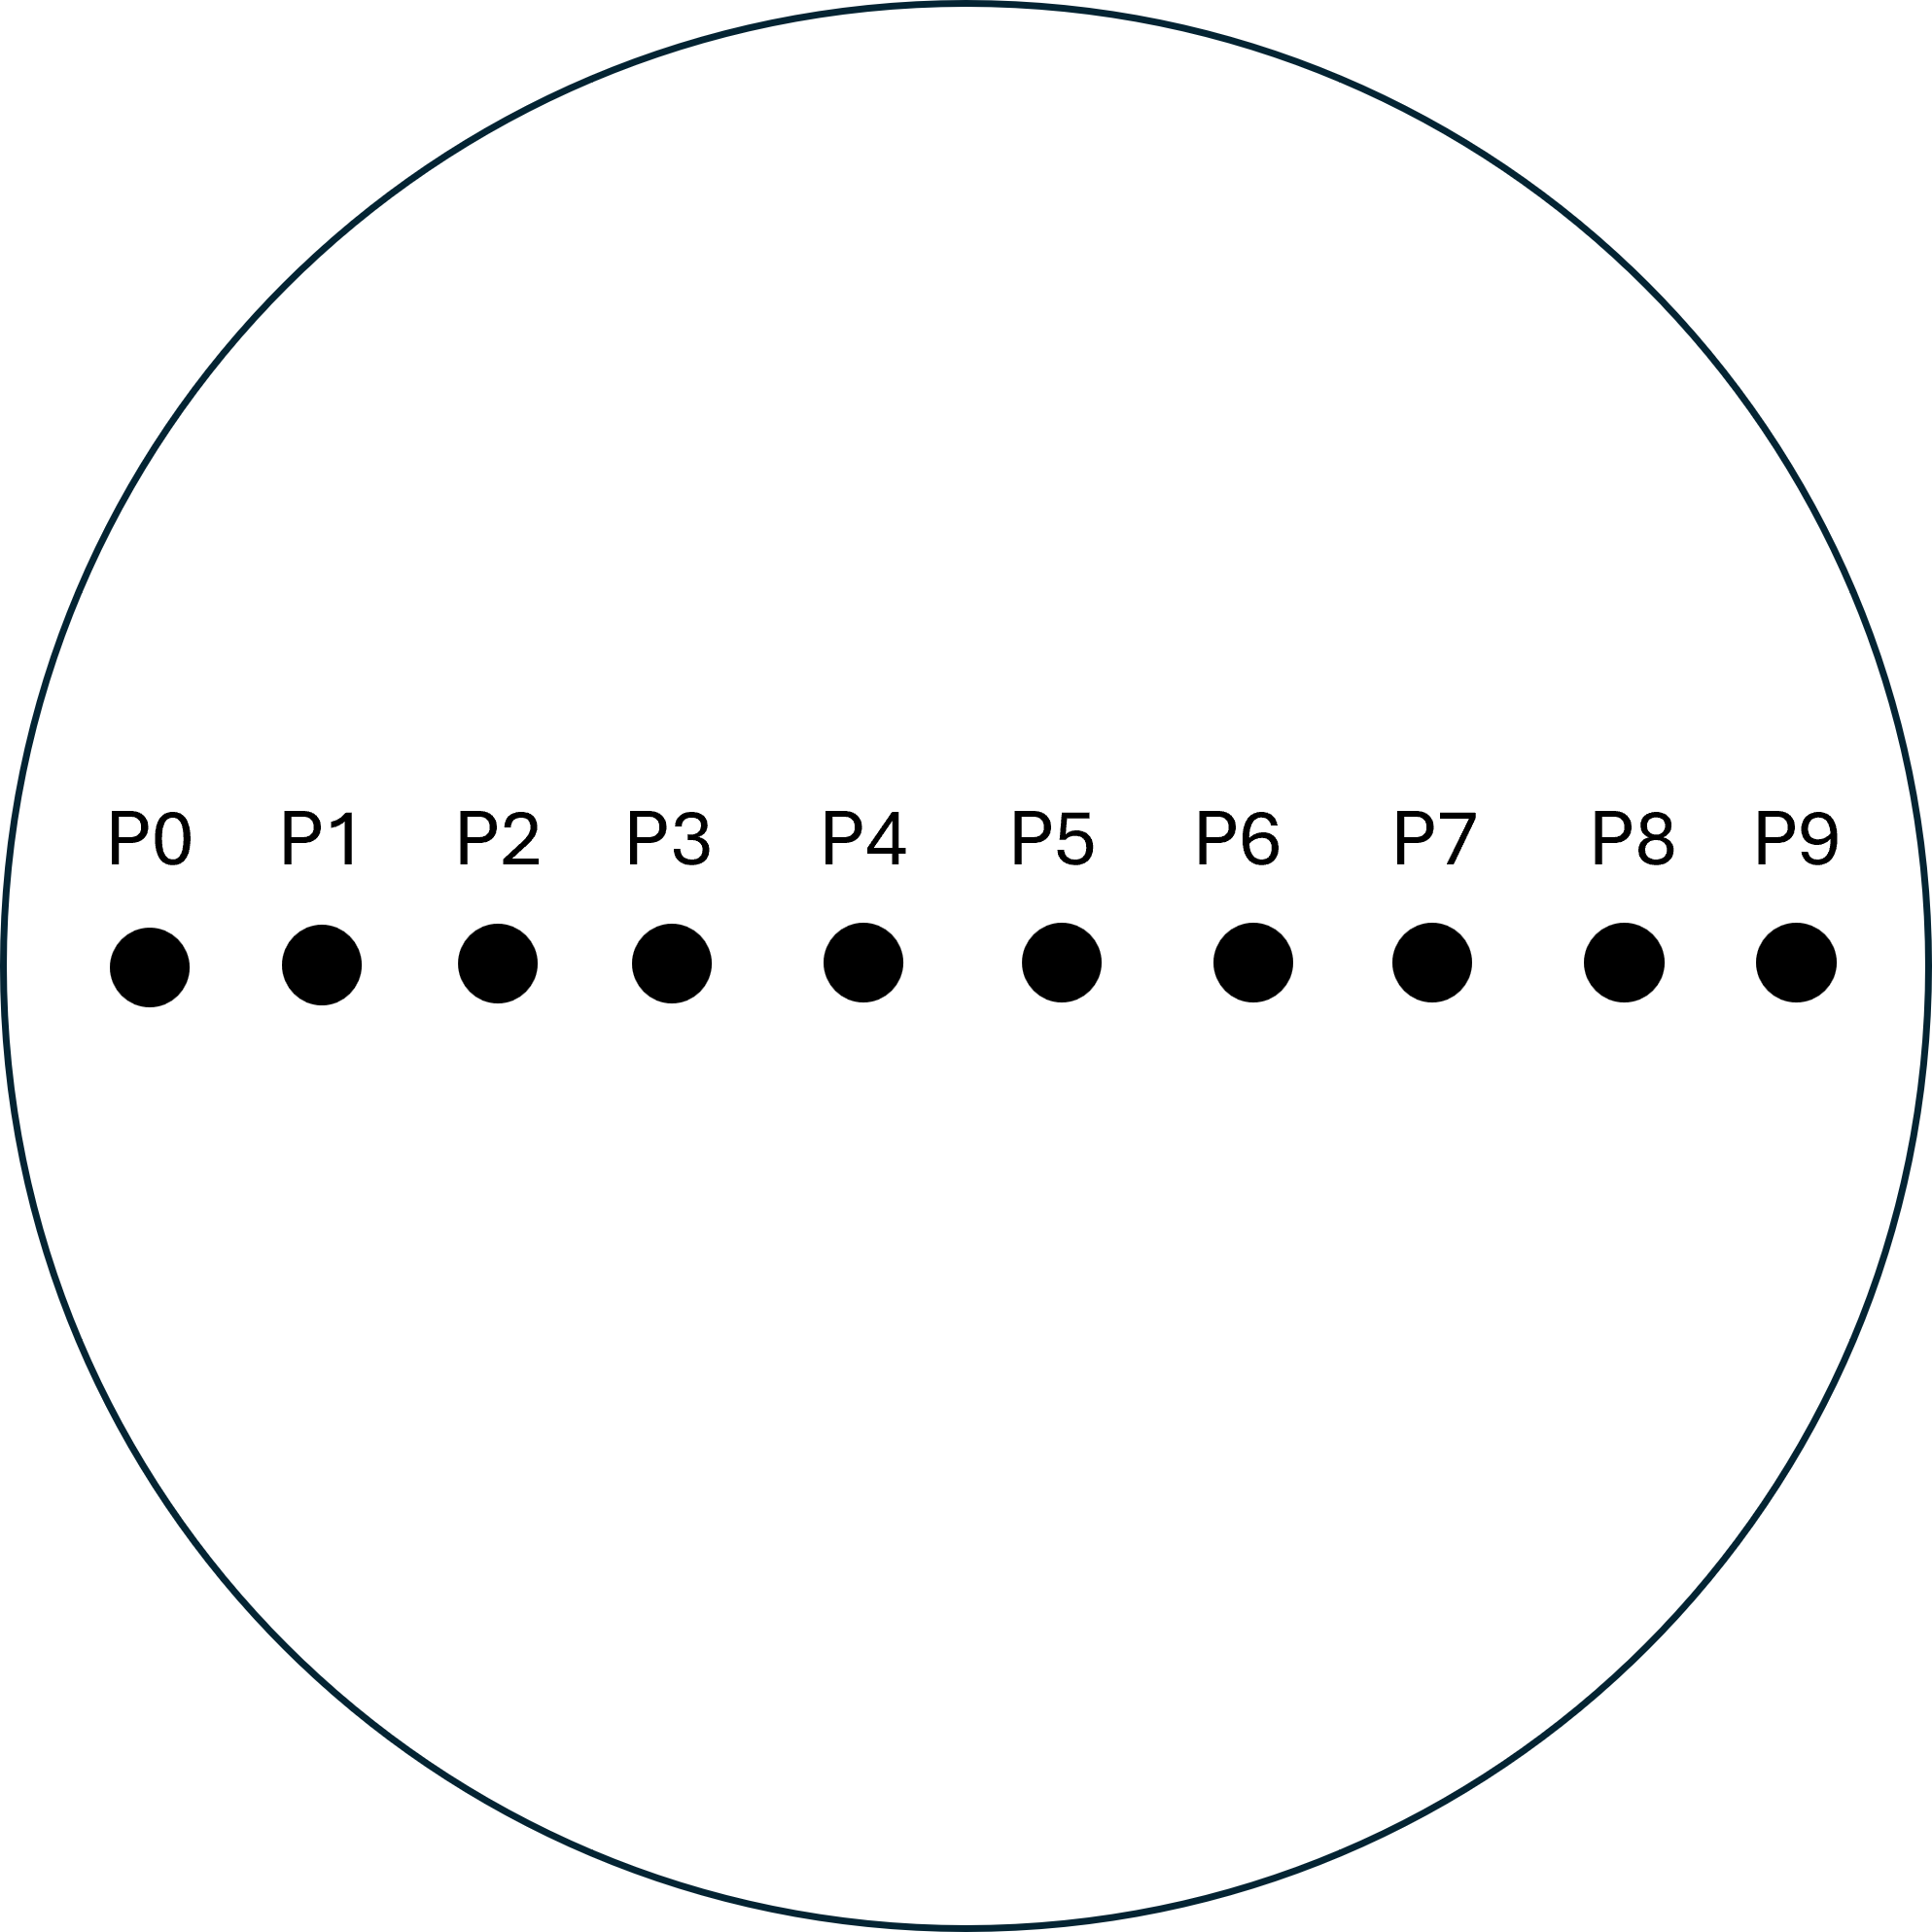
\includegraphics[width=0.5\linewidth]{Figures/probes_points.png}
    \caption{Probes at which pressure and temperature are measured in Figure \ref{fig:pressure_mach_sweep}}
    \label{fig:point_probes}
\end{figure}

\begin{landscape}
    \begin{figure}
        \centering
        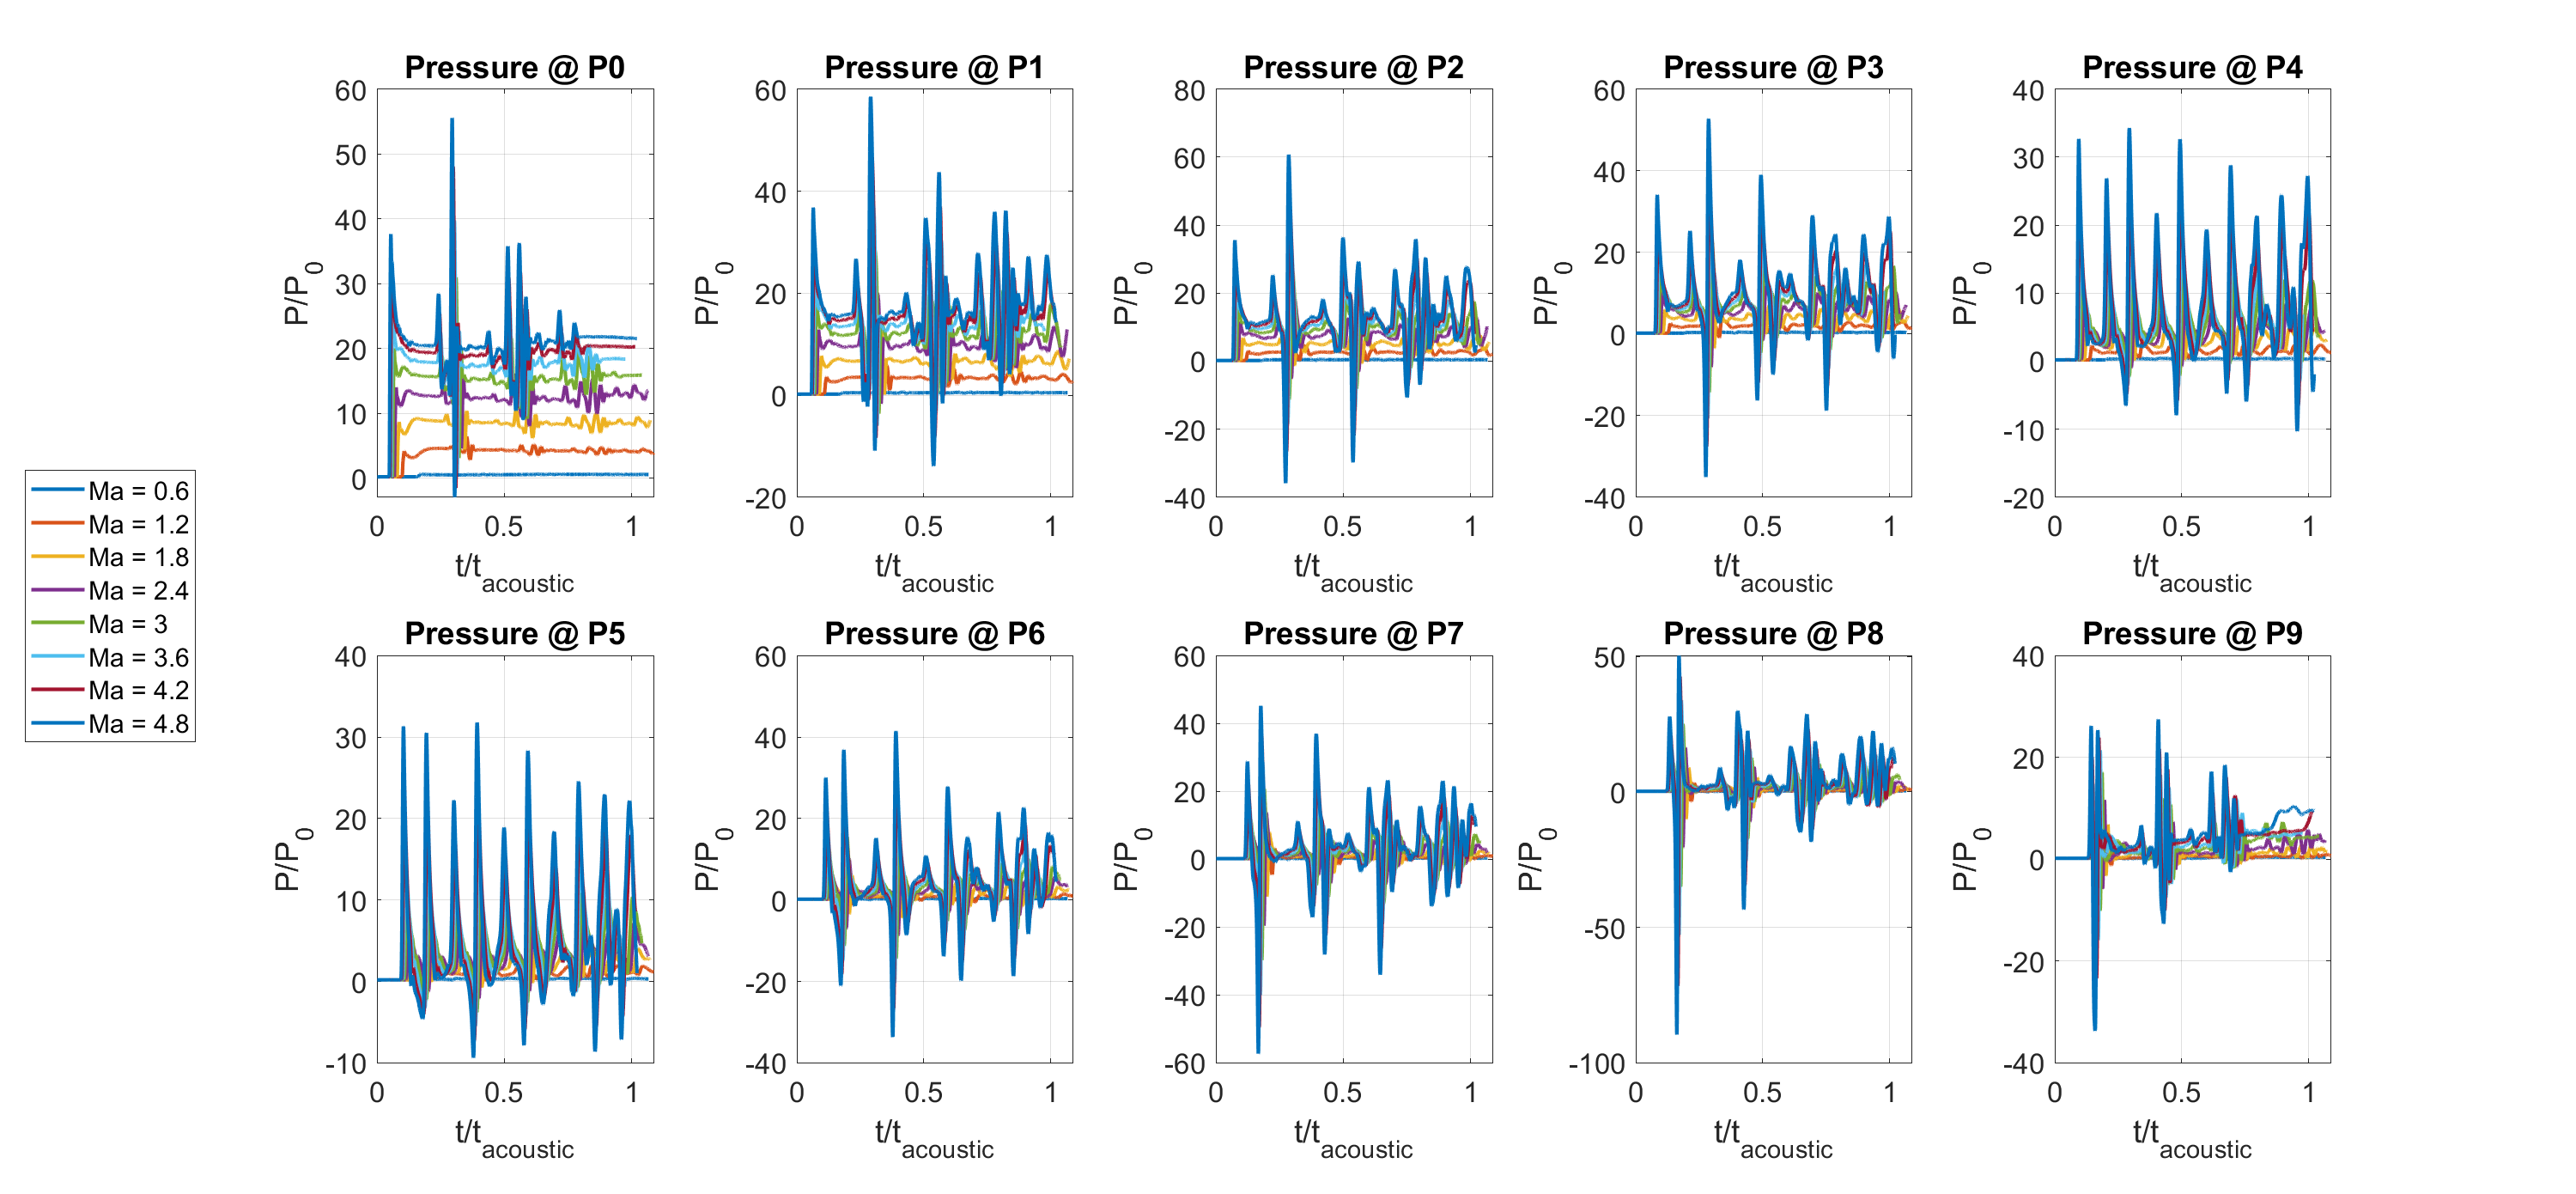
\includegraphics[width=\textwidth,height=\textheight,keepaspectratio]{Figures/pressures_Mach_sweep.png}
        \caption{Normalized pressure measured at probe points throughout the droplet center axis.}
        \label{fig:pressure_mach_sweep}
    \end{figure}
\end{landscape}

\subsection{Deformation Dynamics}
\label{subsec:secondaryDropResults}
The passive scalar described in Equation \ref{eq:secondDropPassiveScalar} and \ref{eq:diffusionSource} was set up in the simulation domain, and ran. Figure \ref{fig:secondaryDropResult} shows the evolution of the position-tracking passive scalar after the droplet begins to experience breakup. 
In Figure \ref{fig:secondaryDropResult} shows that the leading edge of the droplet tends to roll up to the top of the droplet, and hence, the leading edge is the first part of the droplet to atomize via sheet-stripping. The top of the droplet moves downward toward the trailing edge

\begin{figure}[htp!]
\centering
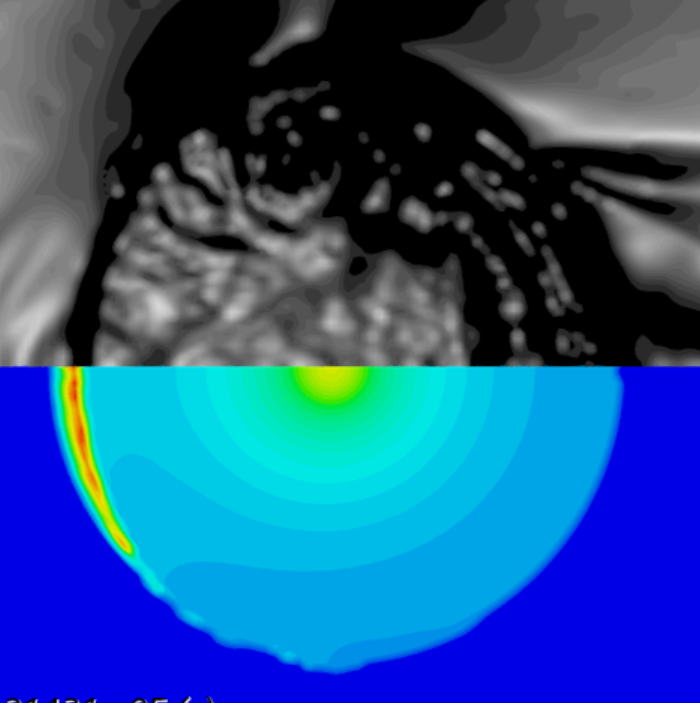
\includegraphics[width=.5\textwidth]{Figures/secondaryDropPassiveScalar.png}
\caption{Position-tracking passive scalar used to track droplet deformation dynamics after the shock has passed through the droplet.}
\label{fig:secondaryDropResult}
\end{figure}

\subsection{Shock-Tracking}
\label{subsec:shockTrackingResults}

The evolution of the passive scalar to track pressure gradient accumulation is shown in Figure \ref{fig:pressureGradScalar}. The shock front is tracked through the minimum of this passive scalar, with a threshold part. Interestingly, the point with the most accumulation in pressure gradient in \ref{fig:t_star_1} corresponds with the point where shear stress begins to build up, as in Figure \ref{fig:shearScalar}, and a point where a Kelvin-Helmholtz instability is seen in an unpublished, high-fidelity simulation result by Rebecca Shannon and Dr. Sheryll Grace at Boston University. This merits further investigation to determine whether the high pressure accumulation may lead to the instability. 

Further work is needed to make this analysis more comprehensive. First, the shear-tracking passive scalar will be altered to ensure it can only accumulate inside the droplet. Also, convection will be turned off for both the pressure and shear passive scalars. To elucidate dominant forces ion the droplet that could be causing instability and breakup, a ratio of pressure force to shear force will be calculated for the cells inside the droplet.

\begin{figure}[htp!]
    \centering
    \begin{subfigure}{0.4\textwidth}
        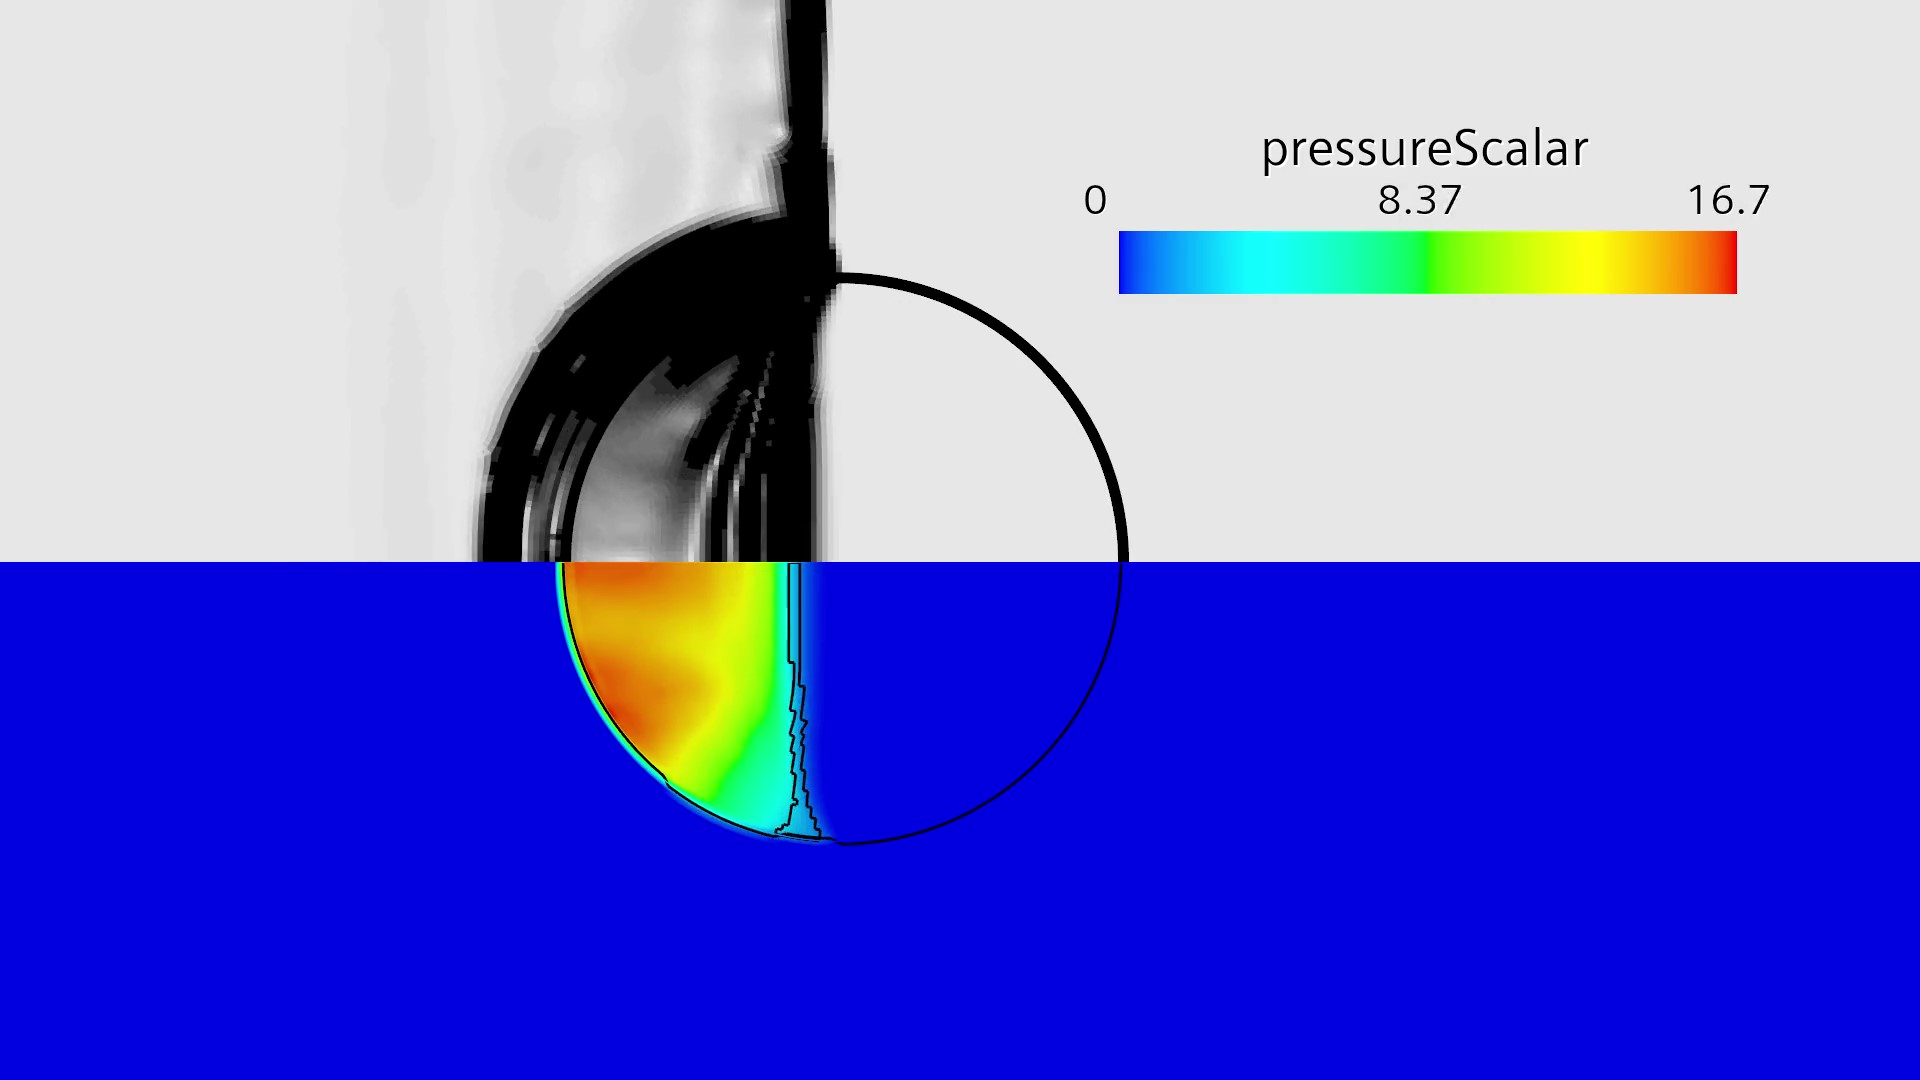
\includegraphics[width=\textwidth]{Figures/pressureGradScalarMiddle.jpg}
        \caption{$t^{*} = 0.5$}
        \label{fig:t_star_0.5}
    \end{subfigure}
    \begin{subfigure}{0.4\textwidth}
        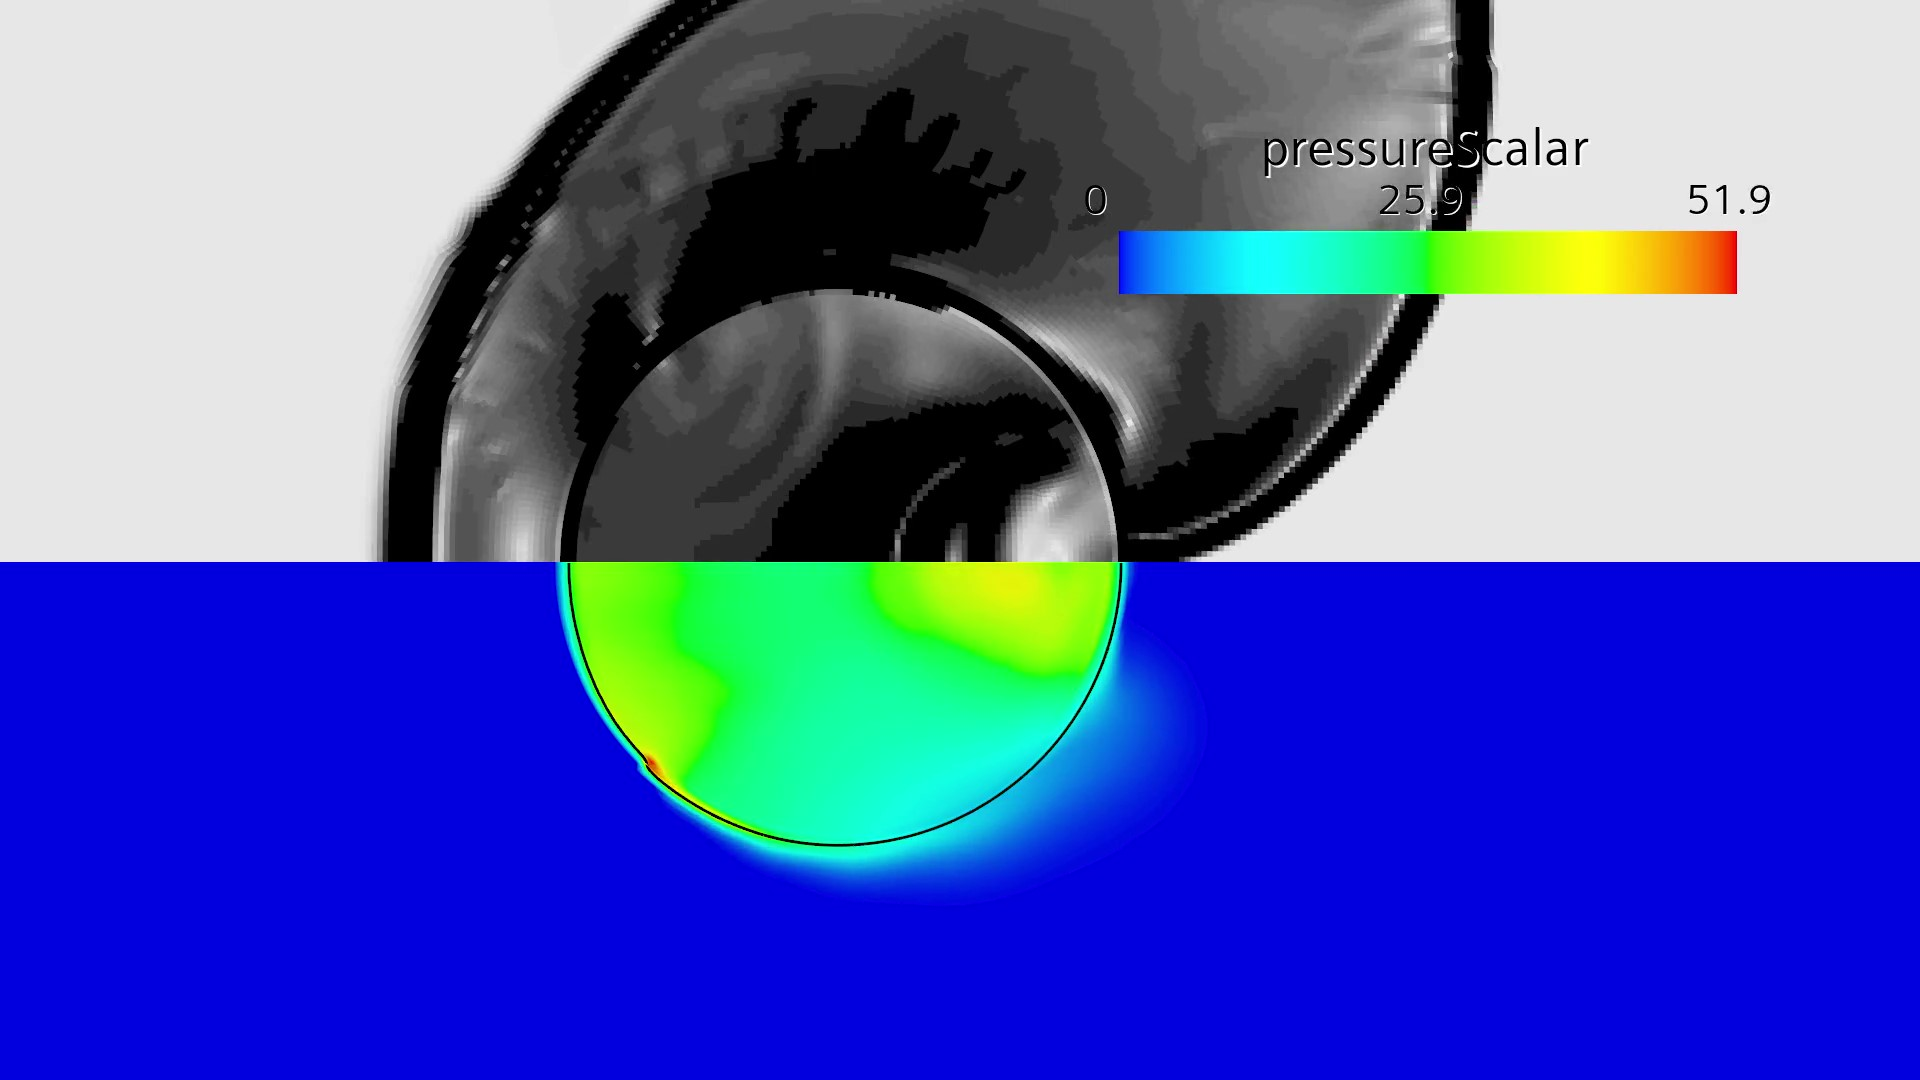
\includegraphics[width=\textwidth]{Figures/pressureGradScalarfinal.jpg}
        \caption{$t^{*} = 1.0$}
        \label{fig:t_star_1}
    \end{subfigure}
    \caption{Evolution of the passive scalar that tracks pressure gradient through time. Here, $t^{*} = 1.0$ is the time it takes for the shock to pass through the droplet. The shock front is also visualized as the minimum value of this passive scalar, as seen by the black outline in \ref{fig:t_star_0.5}}
    \label{fig:shearScalar}
\end{figure}

\begin{figure}[htp!]
    \centering
    \begin{subfigure}{0.4\textwidth}
        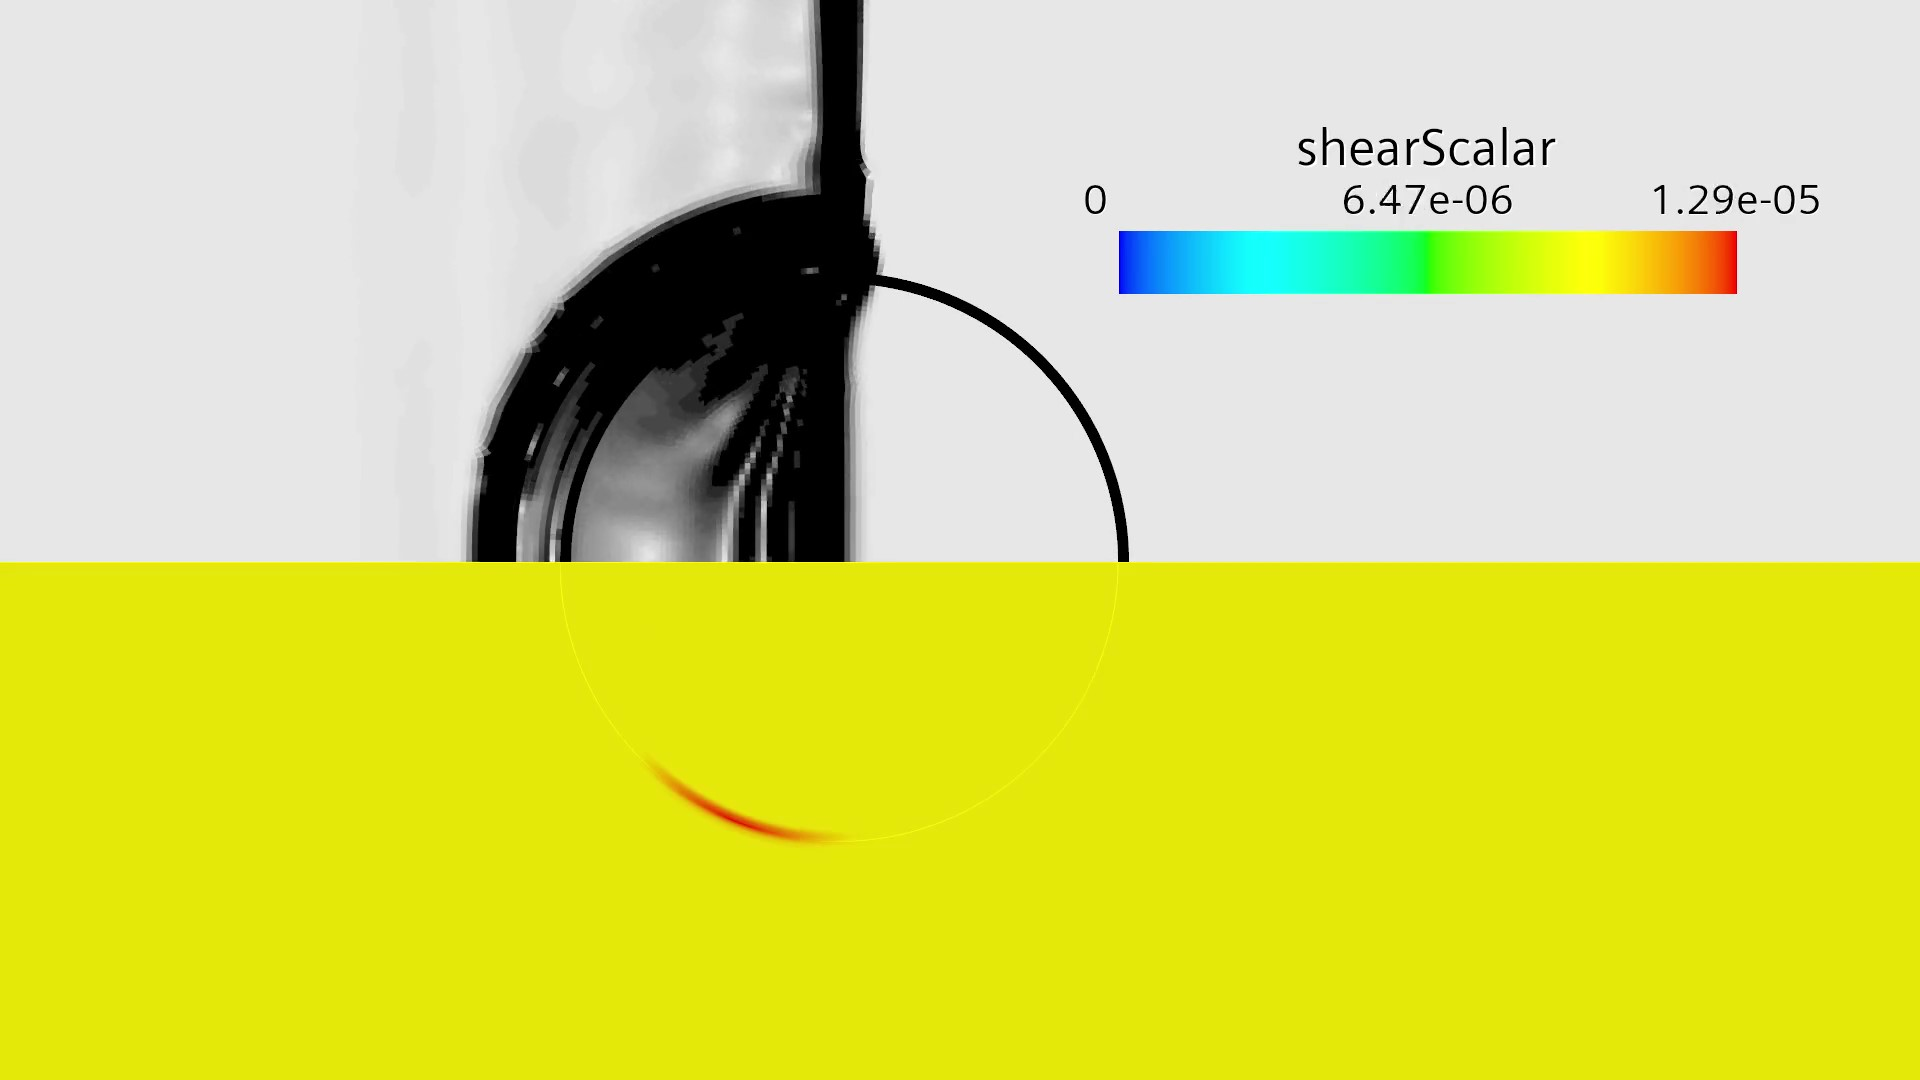
\includegraphics[width=\textwidth]{Figures/shearScalarMiddle.jpg}
        \caption{$t^{*} = 0.5$}
        \label{fig:t_star_0.5_shear}
    \end{subfigure}
    \begin{subfigure}{0.4\textwidth}
        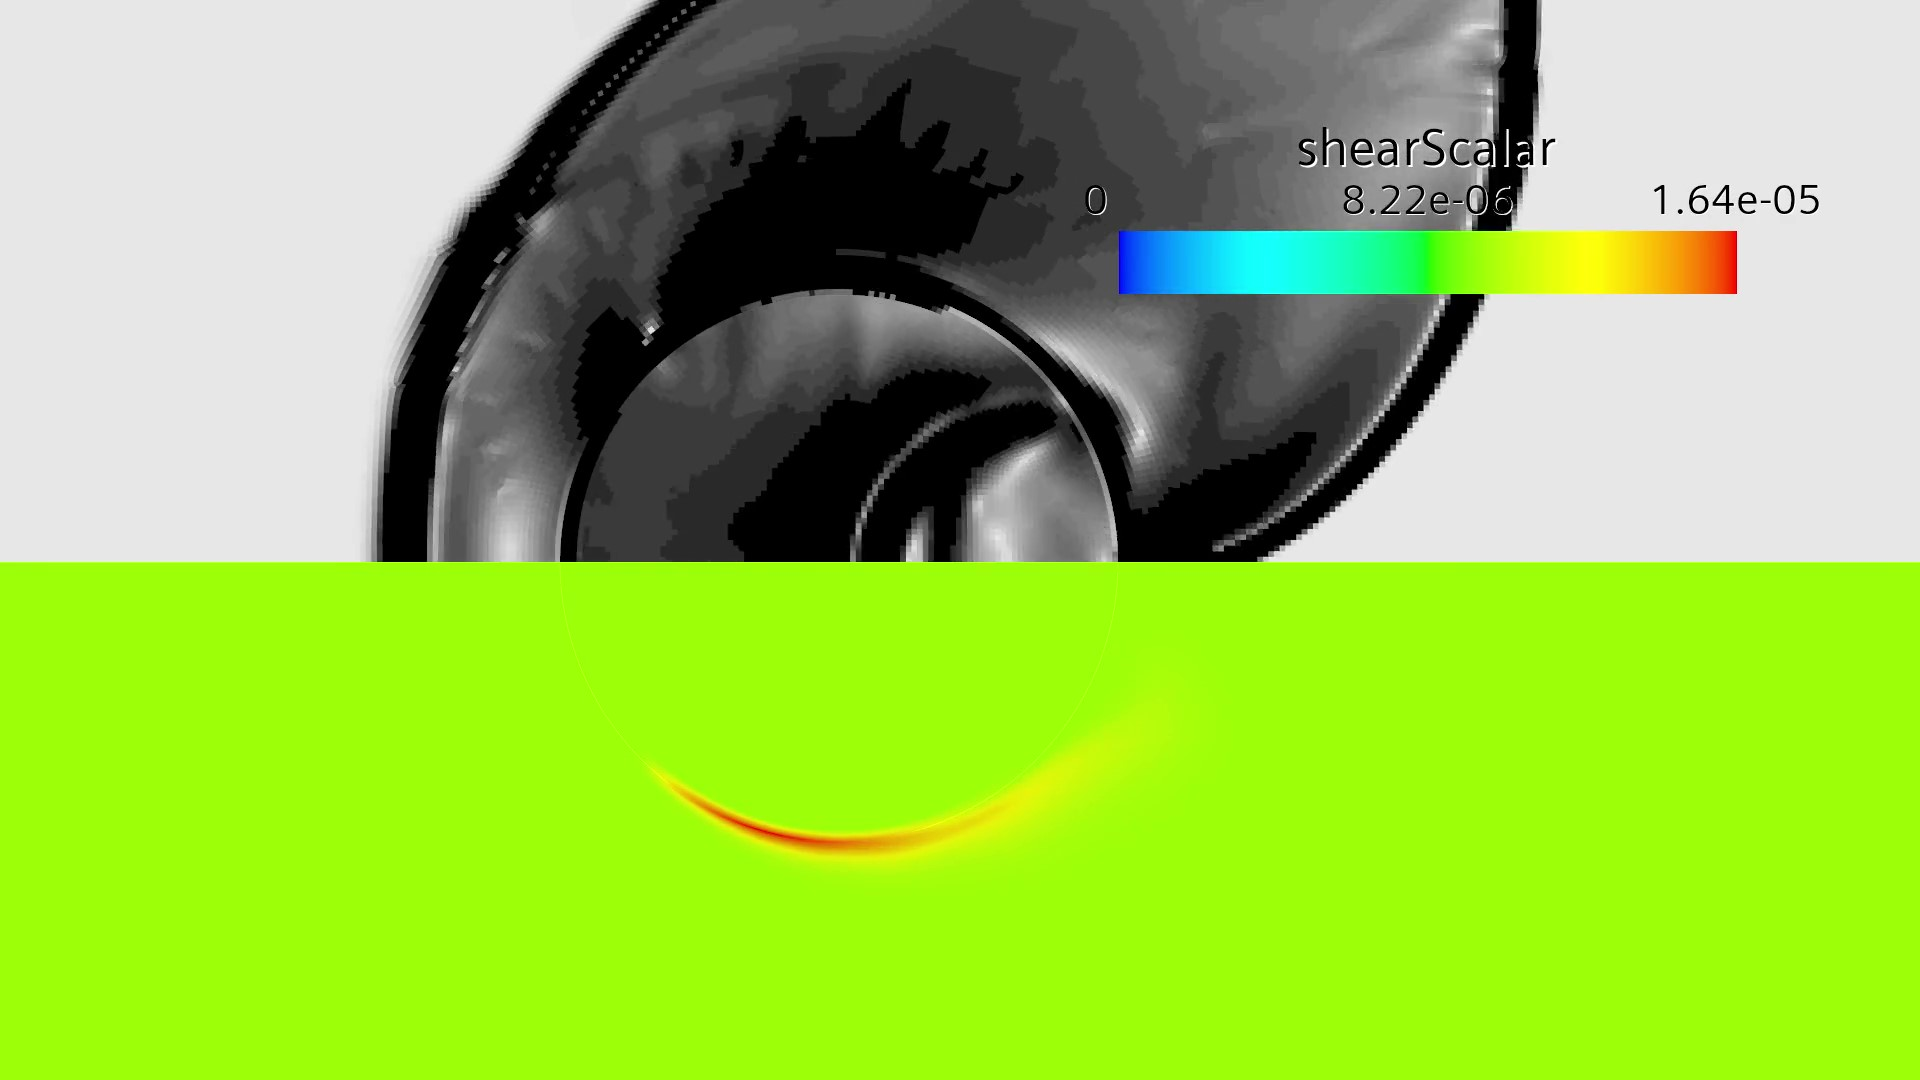
\includegraphics[width=\textwidth]{Figures/shearScalarFinal.jpg}
        \caption{$t^{*} = 1.0$}
        \label{fig:t_star_1_shear}
    \end{subfigure}
    \caption{Evolution of the passive scalar that tracks $\tau_{xy}$. Here, $t^{*} = 1.0$ is the time it takes for the shock to pass through the droplet. Here, it can be seen that the shear stress is built up along the interface of the droplet, and begins to build up around the same point where the highest pressure accumulation occurs in Figure \ref{fig:pressureGradScalar}.}
    \label{fig:pressureGradScalar}
\end{figure}

\subsection{Shape Characterization}
\label{subsec:shapeCharacterResults}

The shape characterization methods described in Section \ref{sec:dropShapeMethod} were used to track the deformation of the droplet as the shock passes through it.The major and minor diameter of the droplet was tracked as a function of time for several $M_{shock}$.
Figure \ref{fig:diameters_v_time} shows how the major diameter decreases with time and the minor diameter increases with time. This result is consistent with the general trend of the Taylor Analogy Breakup (TAB) distortion model \cite{TAB_model}. 

\begin{figure}
\centering
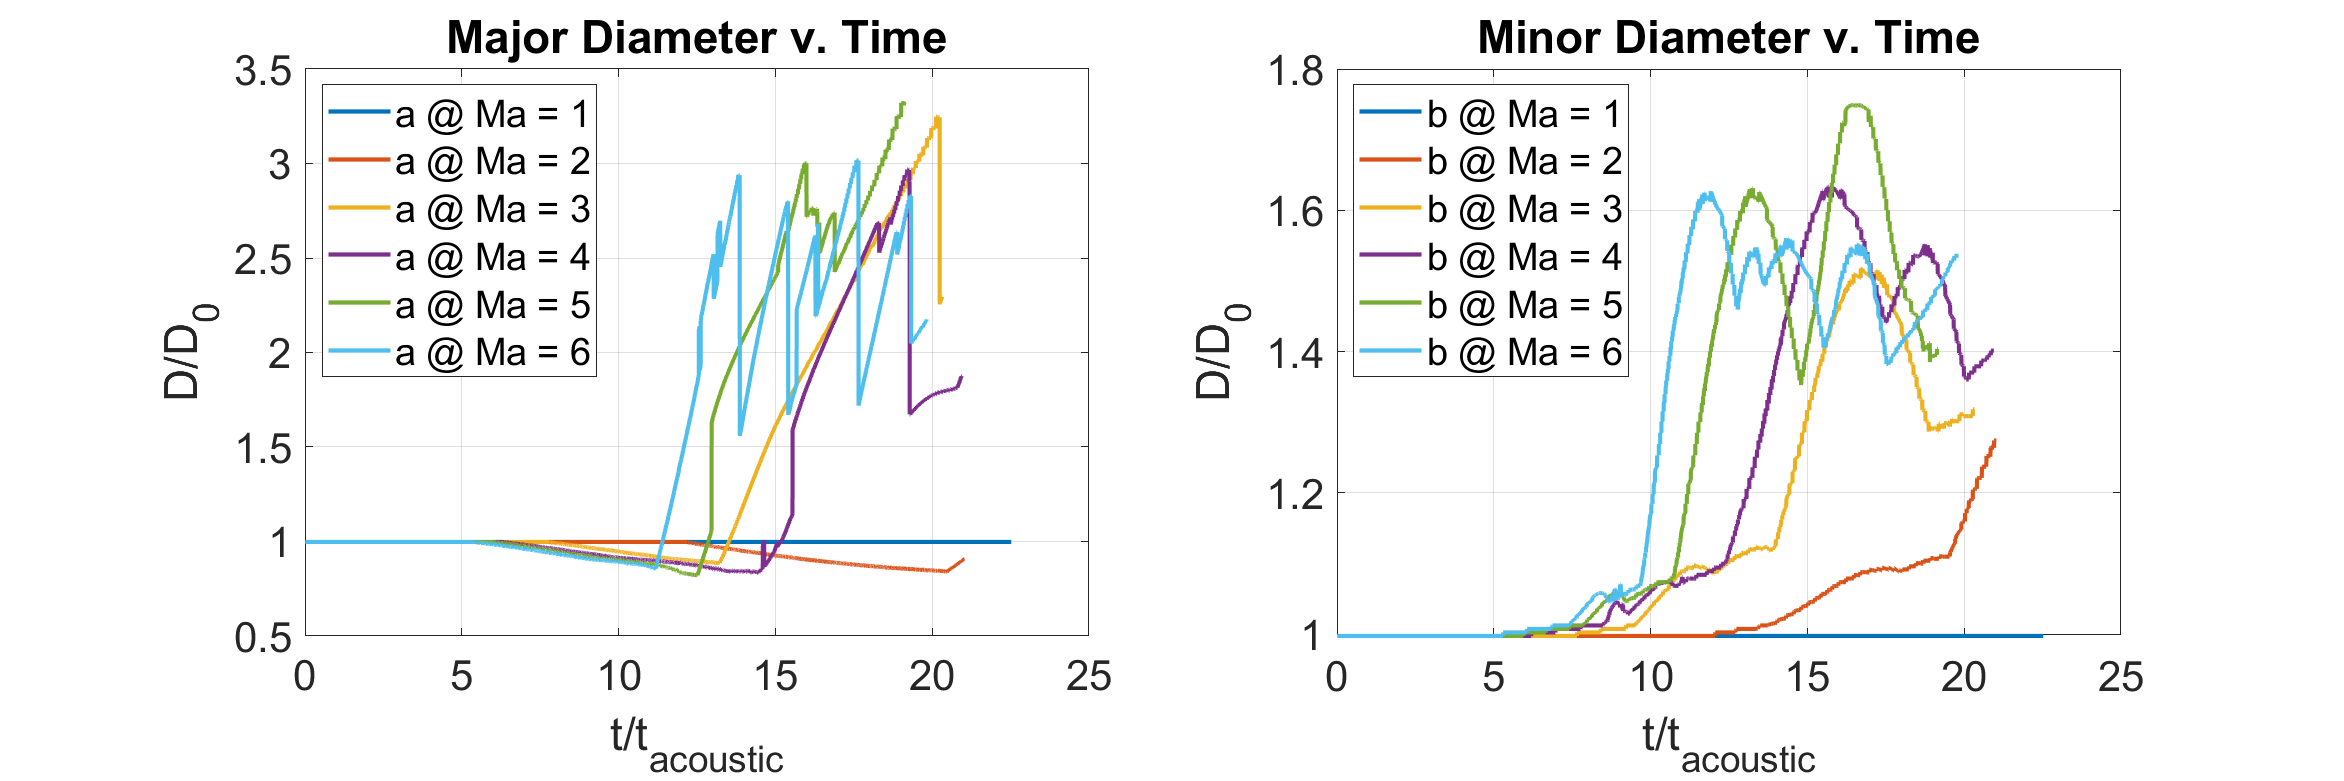
\includegraphics[width=\linewidth]{Figures/Diameters_v_time.png}
\caption{Flattening (Equation~\ref{eq:flattening}) of the droplet as a function of time. This time history is plotted for various $M_{shock}$.}
\label{fig:diameters_v_time}
\end{figure}


The flattening of the droplet (Equation~\ref{eq:flattening}) was continuously calculated before droplet breakup.
Figure~\ref{fig:transientFlattening} shows the flattening of the droplet as a function of time for various $M_{shock}$ and corresponding $We_{droplet}$.
Figure~\ref{fig:transientFlattening} also shows comparative experimental results for selected cases \cite{Briggs2024}. 
We are primarily interested in the time period after the shock moves past the droplet, but before the droplet begins to break up. This is the ``flattening period''.
The time to reach this ``flattening period'' is the deformation time-scale, $t_{deform}$.
The CFD results in Figure \ref{fig:transientFlattening} show that higher $M_{shock}$ leads to an increase in maximum flattening
Figure~\ref{fig:transientFlattening} also shows that higher $M_{shock}$ tends to accelerate the droplet flattening. 
The acceleration in droplet flattening is highlighted in Figure \ref{fig:def_time_scale}.
The relationship between $M_{shock}$ and $t_{deform}$ is clearly nonlinear. In the regime $M_{shock} < 4.0$, $t_{deform}$ has much higher sensitivity to $M_{shock}$ than in the regime $M_{shock} > 4.0$.
To speculate as to why this is the case, we must examine why droplets distort in the first place. 
To do this, we look at droplet distortion in the context of the TAB model \cite{TAB_model}.
Here, O'Rourke says a droplet is analogous to a damped mass-spring system \cite{TAB_model}.
The spring can only absorb so much energy before it must deform.
As $M_{shock}$ increases, it is depositing energy in the droplet more quickly, thus causing it to reach a critical state earlier.


\begin{figure}
\centering
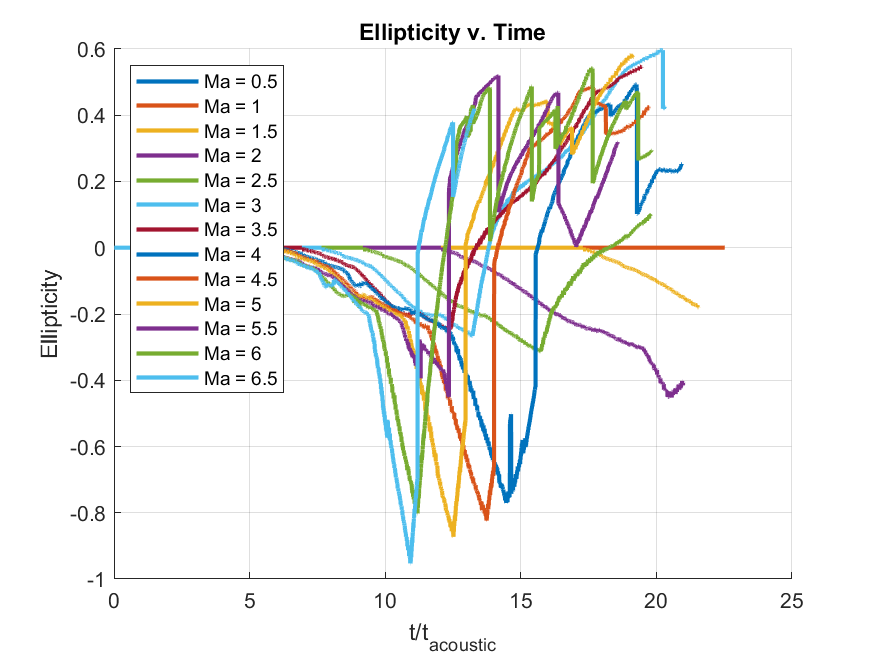
\includegraphics[width=\textwidth]{Figures/Ellipticity_v_Ma.png}
\caption{Flattening (Equation~\ref{eq:flattening}) of the droplet as a function of time. This time history is plotted for various $M_{shock}$.}
\label{fig:transientFlattening}
\end{figure}

\begin{figure}
\centering
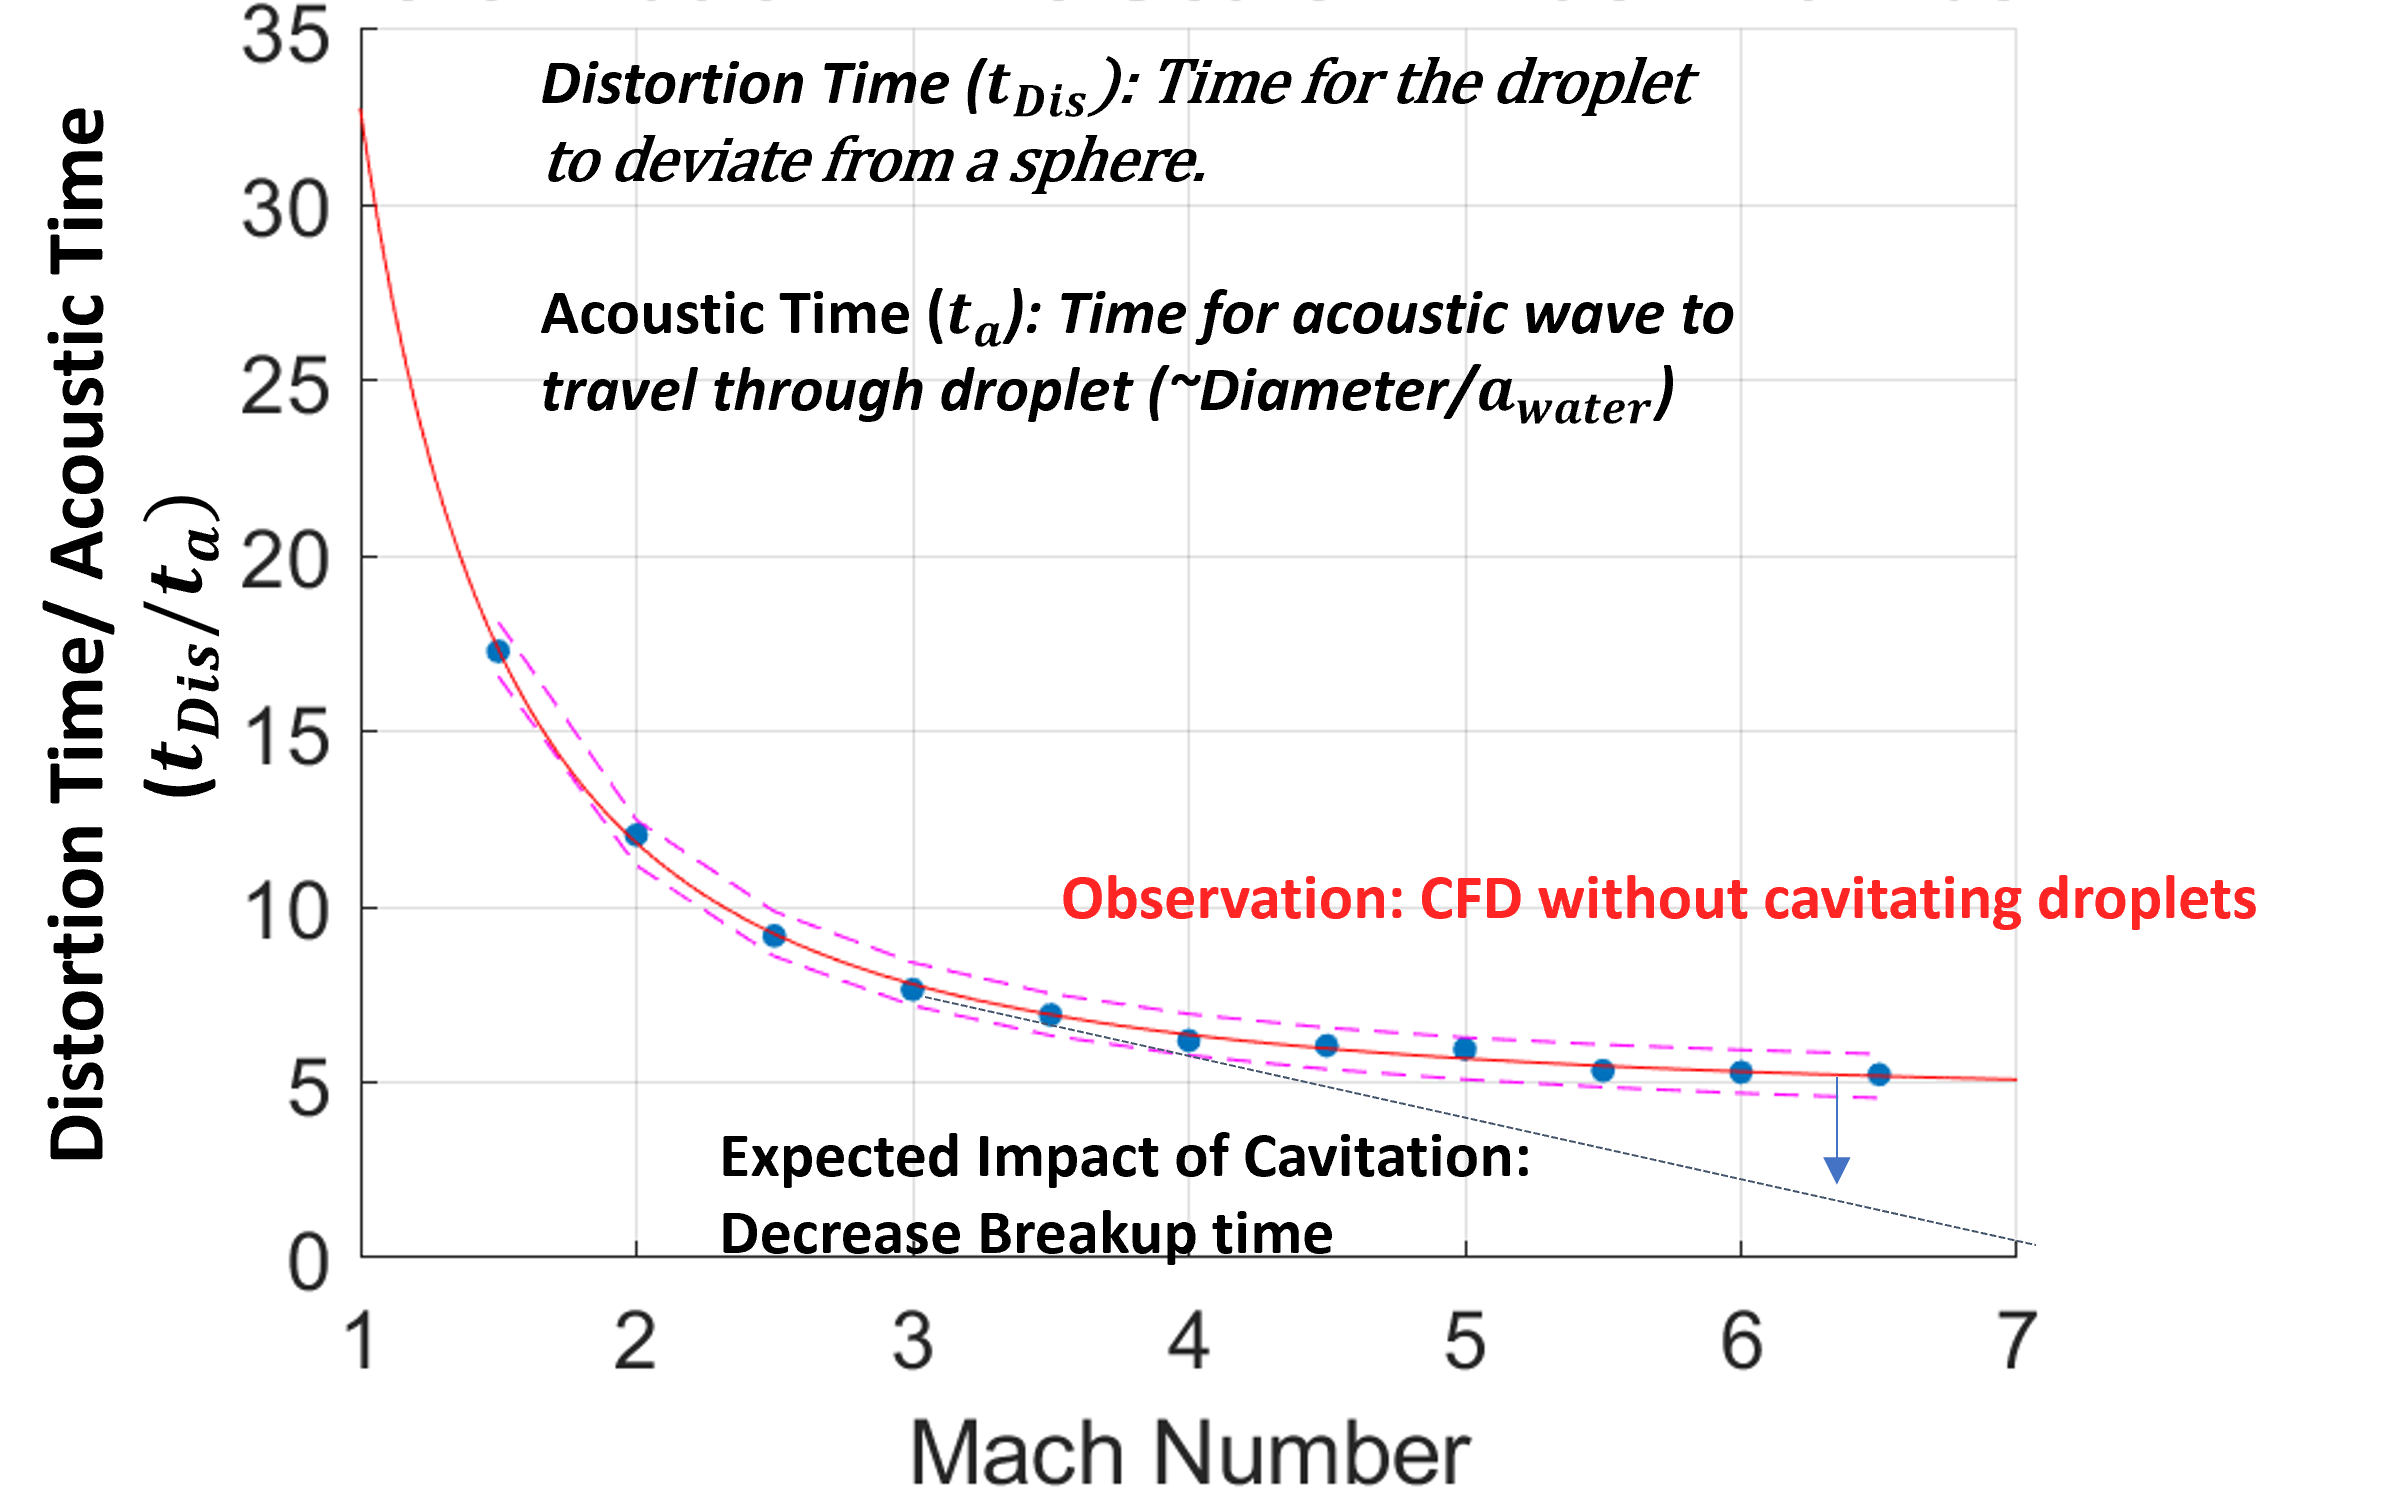
\includegraphics[width=\textwidth]{Figures/Deformation_time_scale_v_Ma.png}
\caption{Time for droplet to begin deformation versus $M_{shock}$.}
\label{fig:def_time_scale}
\end{figure}




\section{CMAS/TBC Infiltration}
\label{sec:CMAS_results}
Here, the results from the simulations and analytical models are discussed, starting with a mesh sensitivity study, moving on to comparing the analytical models with the numerical results, and finally characterization based on several properties is considered.

\subsection{CFD Model}
\subsubsection{Benchmark: Capillary Rise in a Circular Tube}

Since CMAS infiltration in a TBC is a capillary-dominated flow, the methodology above must be validated for use with such flows.
A canonical configuration for a capillary-driven flow is the transient capillary rise in a circular tube.
This case is typically used when validating multiphase numerical methods \cite{GRUNDING2020142, Shiri2022}. 
To do this, a 3D cylindrical tube was set up using the same methods described in Section \ref{sec:CMAS_methods}.
Constant viscosity water with no solidification model was used in place of the molten CMAS, and the domain was isothermal.
The tube's dimensions and boundary conditions are shown in Fig.\ref{fig:benchmark_diagram}. Zero pressure gradient boundaries were used to ensure only capillary forces are driving the flow. Only water was allowed to enter the tube, while water and air can exit the tube.

\begin{figure*}
    \centering
    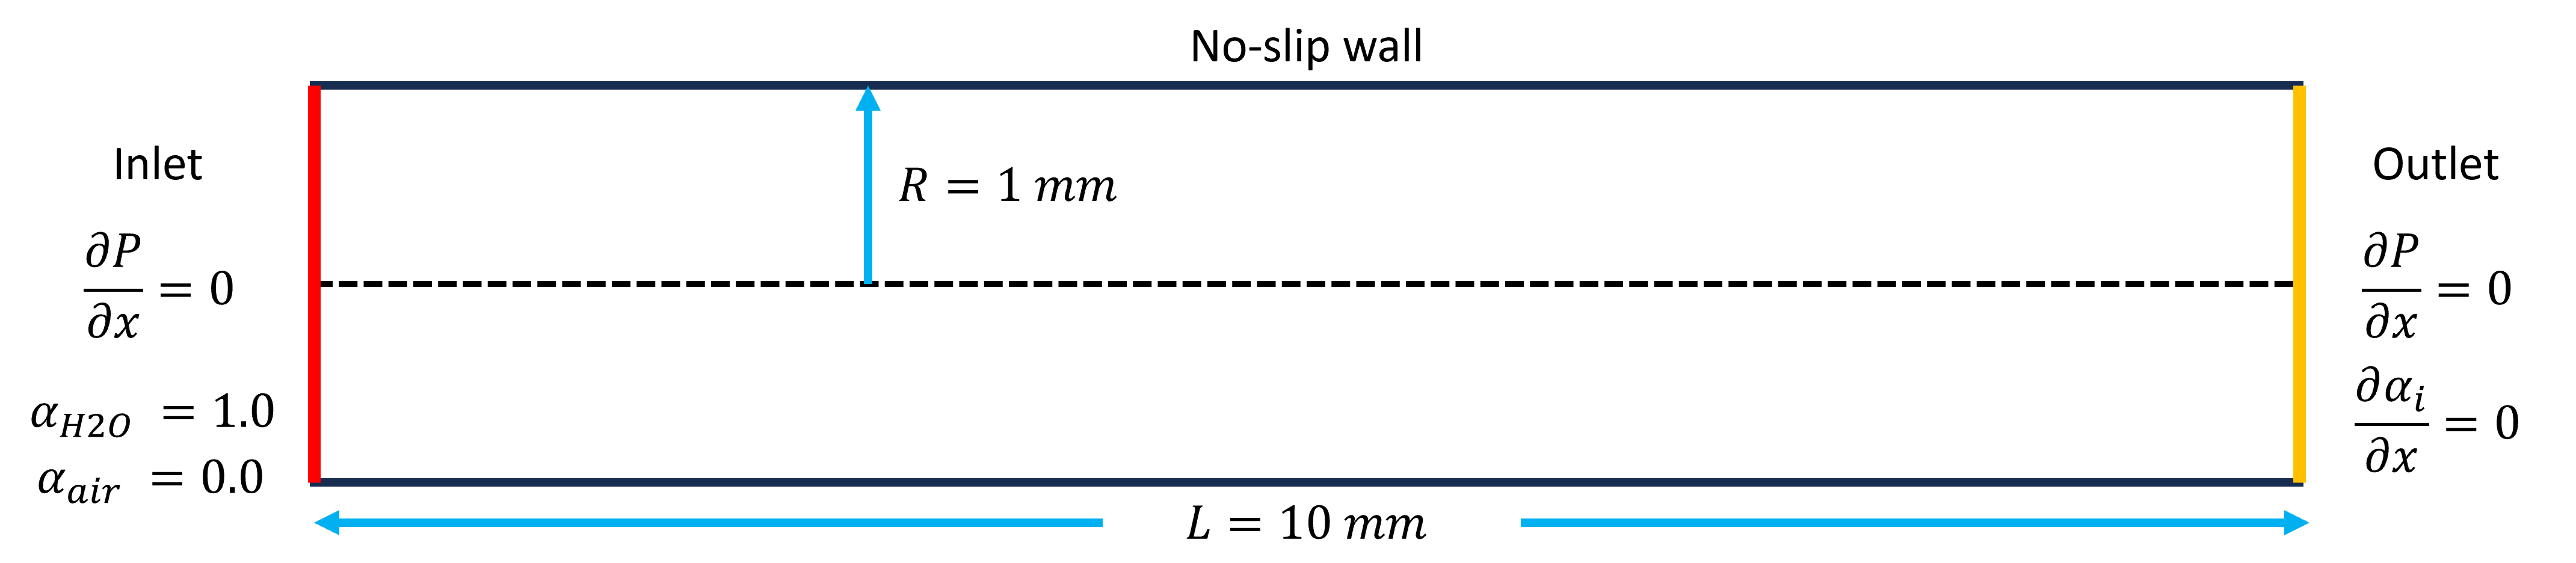
\includegraphics[width=\linewidth]{Figures/capillaryRiseDiagram.png}
    \caption{Diagram showing the dimensions and boundary conditions for the benchmark capillary rise in a tube case.}
    \label{fig:benchmark_diagram}
\end{figure*}

Fig. \ref{fig:capillaryRise} shows the volume fraction of water throughout the capillary rise simulation. Here, a meniscus spontaneously forms due to the capillary action at the tube wall. Then, the meniscus continues to ascend. The ascent rate of the meniscus according to an analytical formulation of the Lucas-Washburn equation \cite{HAMRAOUI2002415} should be around 0.32 $m/s$  (Note that this value was achieved ignoring effects of dynamic contact angle, as this phenomenon is ignored in the present study). The ascent rate of the meniscus in this benchmark CFD model is around 0.36 $m/s$. A 12.5\% error is achieved between the analytical Lucas-Washburn equation and the CFD model. The qualitative observations in Fig. \ref{fig:capillaryRise} and the quantitative comparison between the analytical Lucas-Washburn equation and the CFD model demonstrate the ability of the simulation methodology to resolve capillary-driven flow. 

\begin{figure}
    \centering
    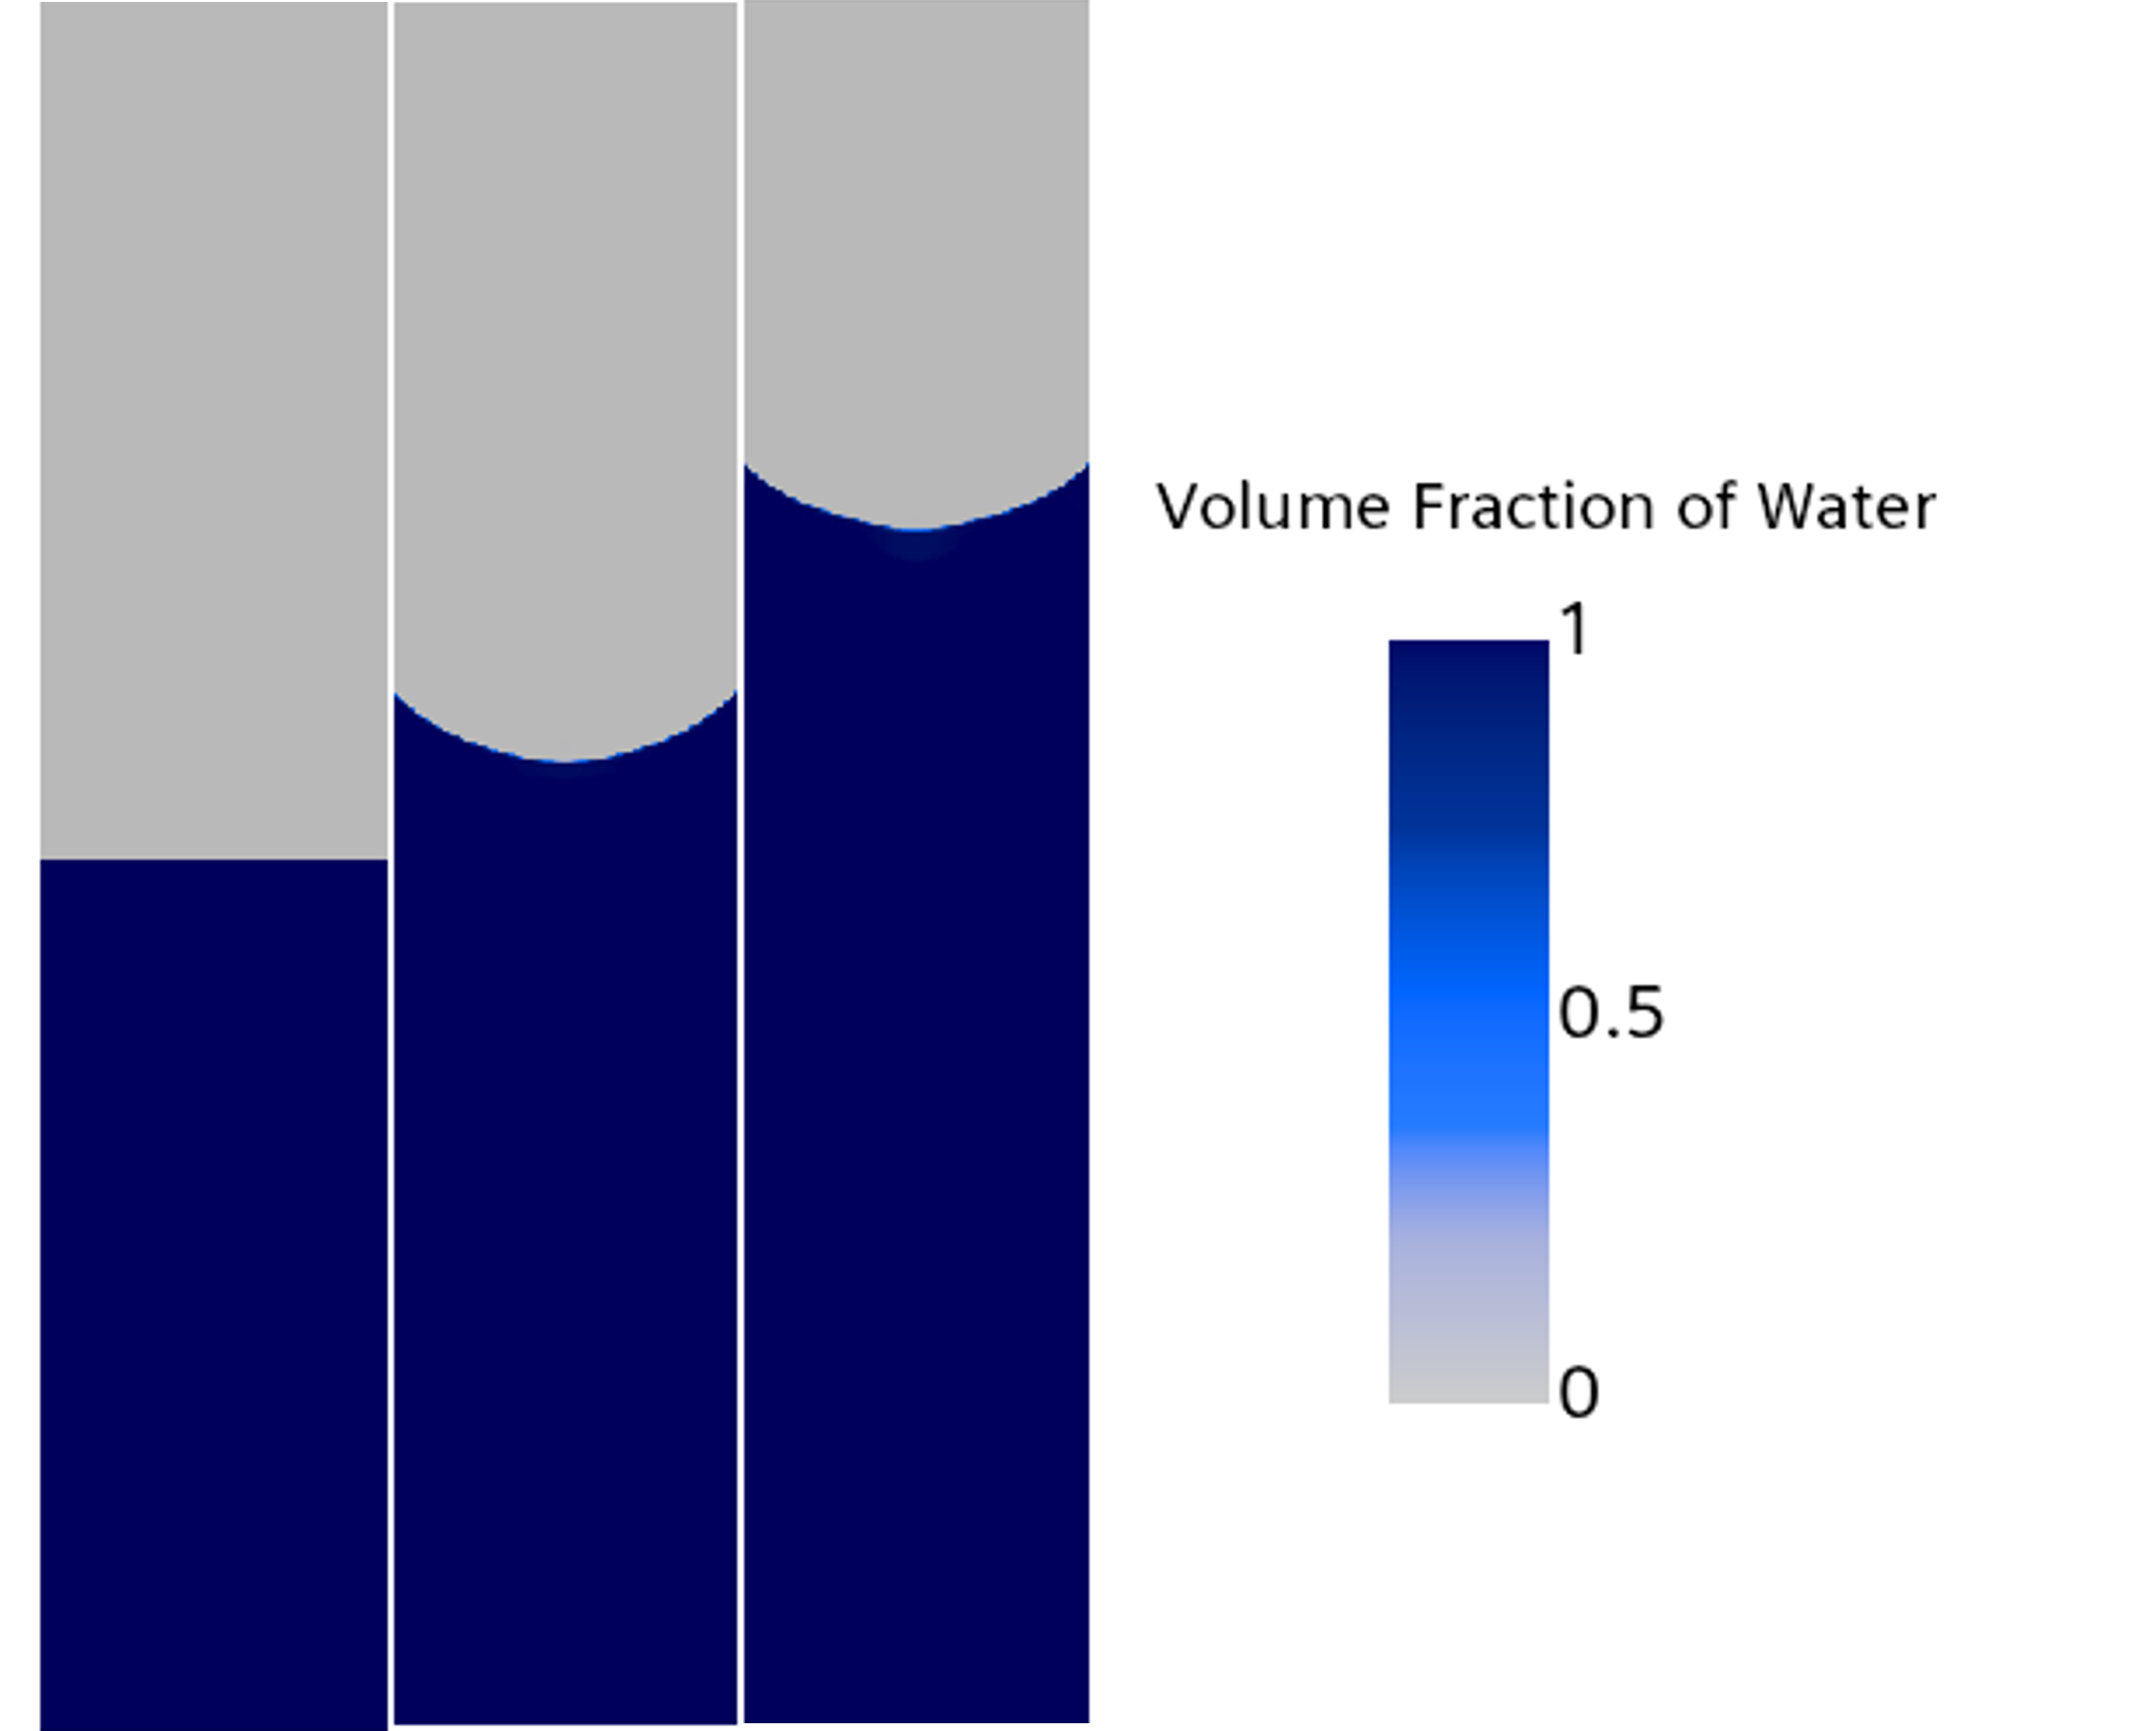
\includegraphics[width=\linewidth]{Figures/validation_capillaryRise.png}
    \caption{Simulated capillary flow in a tube at three different stages. From left to right, the flow is initialized halfway up the tube and there is no meniscus. Next, the meniscus spontaneously forms and begins to move upward. Last, the meniscus has moved much further up the tube than where it started. This shows that capillary rise is resolved.}
    \label{fig:capillaryRise}
\end{figure}

\subsubsection{Validation: Mesh Sensitivity Study}
A mesh sensitivity study was conducted where a single CMAS droplet was resolved. The droplet's initial velocity was 0.2 $m/s$, allowing for quick impingement of the TBC. From there, the droplet infiltrates via capillary action as normal. The setup for this is shown in Fig. \ref{fig:mesh}. The infiltration depth at 0.1 s of physical time was extracted for several levels of refinement. The results in Fig. \ref{fig:meshSensResults} and Table \ref{tab:meshSensResults} show convergence. Since results vary incredibly little with finer mesh sizes, a mesh with a base size of ${1.4\times 10^{-7}}$ m will be used for further simulations. Performing the formal grid convergence index (GCI) calculations \cite{ECA2014104, celik2008procedure} shows that the results in Table \ref{tab:meshSensResults} imply oscillatory convergence, because  $0<\epsilon_{21}/\epsilon_{32}=\ 0.004<1$, and a GCI of $7.5\times 10^{-4}$.
%The physical time to extract the infiltration depth was chosen because beyond that time, error accumulates in the low-fidelity simulation, where the mass of CMAS grows beyond the initial value, causing the result to be non-physical. This non-physical phenomenon can be seen in the coarsest mesh in Fig. \ref{fig:mesh-a}, and the result becomes more clear in Fig. \ref{fig:mesh-b} \ref{fig:mesh-d}. 

% \begin{figure}[htp!]
%     \begin{subfigure}{0.5\linewidth}
%         \centering
%         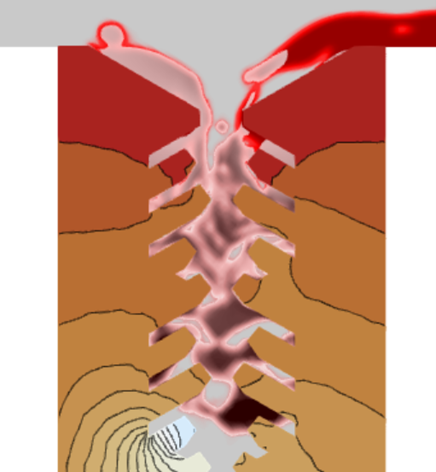
\includegraphics[scale=0.75]{Figures/coarsestMesh.png}
%         \caption{$2.1x10^{-7}$}
%         \label{fig:mesh-a}
%     \end{subfigure}
%     \begin{subfigure}{0.5\linewidth}
%         \centering
%         \includegraphics[scale=0.75]{Figures/fineMesh.png}
%         \caption{$1.4x10^{-7}$}
%         \label{fig:mesh-b}
%     \end{subfigure}
%     \begin{subfigure}{0.5\linewidth}
%         \centering
%         \includegraphics[scale=0.75]{Figures/finerMesh.png}
%         \caption{$1.0x10^{-7}$}
%         \label{fig:mesh-c}
%     \end{subfigure}
%     \begin{subfigure}{0.5\linewidth}
%         \centering
%         \includegraphics[scale=0.75]{Figures/finestMesh.png}
%         \caption{$7.5x10^{-8}$}
%         \label{fig:mesh-d}
%     \end{subfigure}
%     \caption{CMAS Infiltration at different levels of mesh refinement}
%     \label{fig:mesh-refine}
% \end{figure}

\begin{figure}
    \centering
    \includegraphics[width=\linewidth]{Figures/infilDepthMesh.png}
    \caption{Infiltration Depth ($\mu m$) as a function of the inverse of representative mesh size ($\mu m ^{-1}$)}
    \label{fig:meshSensResults}
\end{figure}

\begin{table}[htp!]
    \centering
    \caption{Mesh Sensitivity Results from Fig. \ref{fig:meshSensResults}}
    \begin{tabular}{c|c}
       Representative Mesh Size (m)  & Infiltration depth at 0.1 s (m) \\
       \hline
        $2.1\times10^{-07}$ & $4.475\times10^{-05}$ \\
        $1.4\times10^{-07}$ & $3.281\times10^{-05}$ \\
        $1.0\times10^{-07}$ & $3.232\times10^{-05}$ \\
        $7.5\times10^{-08}$ & $3.238\times10^{-05}$
    \end{tabular}
    \label{tab:meshSensResults}
\end{table}

\subsubsection{2D CFD Model}
In Section \ref{sec:CMAS_methods}, it is mentioned that the boundary conditions on the 2D model make it such that it is not strictly a capillary-driven flow, but also inertially-driven. This has unintneded consequences on the results. The limitations in the 2D model causes the flow to reach a state of equilibrium, as seen in Fig. \ref{fig:rect_v_feather}. This phenomenon is non-physical, since the CMAS should continue to infiltrate instead of reach a point of equilibrium \cite{Naraparaju2017}. So, the 2D geometry cannot be used to ``resolve'' the infiltration process. However, it is still valuable in the sense that it can demonstrate a microstructure's ability to stop the infiltration under different circumstances.

To understand the effect of geometry, the 2D CFD results from the rectangular and feathery channel geometries are shown in Fig. \ref{fig:dimensions}.
Additionally, the 2D CFD results are compared to analytical solutions of the open-pipe and concentric-pipe models (OPM, and CPM respectively) \cite{Naraparaju2019} based on models detailed in Appendix \ref{sec:RaviPipeModels}. 
Fig.~\ref{fig:rect_v_feather} shows the infiltration depth versus time for the rectangular and feathery simulations, co-plotted with the analytical OPM and CPM solutions. 
Note that the CFD results in Fig.~\ref{fig:rect_v_feather} account for a fluidic viscosity that varies with temperature which is based on polynomial fit to experimentally-measured data \cite{Naraparaju2017}.\\

First, consider the rectangular and feathery CFD data in Fig.~\ref{fig:rect_v_feather}.
These CFD results show that the feathery channel works to mitigate infiltration as compared to the rectangular channel. Such an inference can be drawn from the CMAS infiltrating to shallower depths for the feathery channel compared to the rectangular channel. 
% Next, consider the circular and annular CFD results in Fig.~\ref{fig:rect_v_feather}, which differ as they depict a constant value for both cases.
% These differences are associated with the CMAS flow in the circular and annular channels results reaching an equilibrium at essentially the initial condition. 
% Such a result may seem counter-intuitive at first, however, it is supported by capillary flow theory.
% Capillary flow in small tubes is driven by the inertial response time \cite{Weislogel}, $t_{R}  \thicksim \sqrt{\frac{\rho R^{3}}{\sigma}}$; since the radius of the tube is small, the inertial response time is on the order of $1\times 10^{-9} s$. This is much smaller than the minimum time-step of the CFD simulations.
% Therefore, CMAS infiltration flow reaches an equilibrium immediately.
%Experimental results \cite{Naraparaju2019} for infiltration depth versus time are compared to simulations. These experimental results come from the German Aerospace Center, and the material used for “CMAS 1” is consistent with the material defined in the simulation. Unfortunately, the data is much farther advanced in time and with much less time resolution than the simulation. 


To understand the evolution of CMAS attack, the time history of the CMAS distribution is discussed. 
The effort starts with data extracted from the CFD results. The CFD time history is plotted in Fig.~\ref{fig:rect_v_feather} and, at several points of interest in time, contour plots of the CMAS volume fraction and TBC temperature are plotted in Fig. \ref{fig:feathery_timehistory}. In the contour plots, the red/gray area shows the distribution of air and CMAS, and the red-orange gradient shows the temperature distribution within the TBC (with isocontours in intervals of 1 K). First, consider the initial infiltration in both the rectangular and feathery channels on a time interval from $t=0$ to $t=0.001 s$ in Fig.~\ref{fig:rect_v_feather}.
This early infiltration occurs much faster and the rate of infiltration appears to significantly slow down thereafter. 
Such an fast infiltration occurring early is a result of the conical shape of the micro structure in the coating, shown in Fig.~\ref{fig:feathery_timehistory}. It appears to work much like a converging nozzles, where the flow accelerates with the reduction of the cross-sectional, interstitial area. 

Now consider a later time interval range from $t=0.001 - 0.13 s$ in Fig.~\ref{fig:feathery_timehistory}.
At $t \approx 0.05s$, the infiltration rates of the rectangular and feathery channels diverge.
There, the infiltration in the rectangular channel continues at a faster rate than in the feathery channel.
At $t \approx 0.13 s$, the CMAS in the feathery channel reaches an equilibrium state and no longer infiltrates. Concurrently, the infiltration in the rectangular channel shows a trend that indicates it begins to slow down.
Lastly, after $t \approx 0.15 s$, the infiltration in the rectangular channel eventually reaches an equilibrium as well.
It is important to emphasize that the infiltration in the feathery channel reaches an equilibrium faster and penetrates to shallower depths than in the rectangular channel.
Such an observation is consistent with previous experimental results \cite{Naraparaju2017} and further demonstrates the effectiveness of feathery TBCs to resisting CMAS attack.

In further evaluation of the results, it can be observed from Fig. ~\ref{fig:feathery_timehistory} when focusing on the distribution of air and CMAS that air pockets form within the infiltrated CMAS.
With respect to this, recall that the the thermal conductivity of air is $1-2$ orders of magnitude lower than that of the TBC and CMAS (depending on the temperature). Such air pockets can also not support convection. Hence, the air pockets potentially contribute to a decrease of thermal conductivity in a TBC that has experienced CMAS attack.

In Fig.~\ref{fig:feathery_timehistory}(center) and ~\ref{fig:rect_timehistory}(center), a developing temperature profile is seen within the TBC. The temperature profile develops as energy is absorbed by the CMAS moving downward and that energy is conducted back into the TBC. 
In Fig.~\ref{fig:feathery_timehistory}(right), after further infiltration, the temperature profile switches directions along the TBC interface.
This happens because more energy is being redirected to satisfy the latent heat of fusion of CMAS. The CMAS is effectively cooling the TBC.
This effect is less drastic in Fig.~\ref{fig:rect_timehistory} because there is overall less infiltrated CMAS available for energy absorption.

One discrepancy between these results and previous work is that the meniscus of the CMAS/air interface is convex in Figures \ref{fig:feathery_timehistory} and \ref{fig:rect_timehistory}. Previous work suggests that this meniscus should be concave \cite{Naraparaju2019}. This discrepancy is likely caused by the initial condition in the CFD simulation. That is, the flow is driven by a pressure gradient and capillary action, as opposed to being driven by capillary action from the start. Another discrepancy between experiments, analytical models, and 2D CFD is that the CMAS in the 2D CFD model reaches a state of equilibrium, rather than continuing to infiltrate. This limitation could be fixed with more mesh resolution at the CMAS/Air interface so that the capillary action is properly resolved, but the numerical methods being used here do not support AMR in 2D simulations. Hence, a 3D model is necessary to properly resolve the capillary-driven part of this phenomenon. 

% \begin{figure}[h!]
%     \centering
%     \includegraphics[width=0.75\linewidth]{Figures/analyticalBenchmark.png}
%     \caption{Comparison of Simulation Results to Analytical Models for infiltration depth}
%     \label{fig:analytBench}
% \end{figure}

\begin{figure}
    \centering
    \includegraphics[width=\linewidth]{Figures/2d_results.png}
    \caption{Comparison of infiltration depth versus time for the 2D CFD model's rectangular and feathery micro-channels co-plotted with the analytical pipe model results. Note that the feathery channel reaches an equilibrium at shallower depths at a shorter time than the rectangular channel.}
    \label{fig:rect_v_feather}
\end{figure}

\begin{figure*}
    \centering
    \includegraphics[width=\linewidth]{Figures/featheryTimeHistory.png}
    \caption{Time history of the feathery TBC simulation showing the volume fraction of CMAS and the temperature of the TBC (for $Oh_{initial} \approx 115$ to $Oh_{final} \approx 1300$). The left ($t \approx 2\times 10^{-5}s$) image shows the initial conical infiltration, the middle image ($t\approx 0.005 s$) shows CMAS as it infiltrates the feather arms, and the right image ($t \approx 0.13 s$) is the equilibrium point. Note that the isolines in the TBC represent the thermal gradient, where the temperature at each isoline is 1 K less than the one above it.}
    \label{fig:feathery_timehistory}
\end{figure*}

\begin{figure*}
    \centering
    \includegraphics[width=\linewidth]{Figures/rect_timeHistory.png}
    \caption{Time history of the rectangular TBC simulation showing the volume fraction of CMAS and the temperature of the TBC (for $Oh_{initial} \approx 115$ to $Oh_{final} \approx 1300$). The left image ($t \approx 1\times 10^{-5}s$) shows the initial conical infiltration, the middle image ($t \approx 0.1 s$)shows CMAS as it infiltrates the thin rectangular channel, and the right image ($t \approx 0.4 s$) is the equilibrium point. Note that the isolines in the TBC represent the thermal gradient, where the temperature at each isoline is 1 K less than the one above it.}
    \label{fig:rect_timehistory}
\end{figure*}

% The results from the experiments, pipe models, and the simulation are summarized in Table \ref{tab:resultsSummary}.

% \begin{table}[htp!]
%     \centering
%     \caption{Summary of Analytical, Numerical, and Experimental Results. Note that the simulated result is extrapolated to the same time as the experiments and models, because the simulation result is asymptotic at t = 0.5 s}
%     \begin{tabular}{c|c|c}
%        -  & Time (s) & Depth ($\mu m$)\\
%        \hline
%         Experiment & 120 & 125\\
%         Open-pipe & 120 & 176\\
%         Closed-pipe & 120 & 95\\
%         rectangular micro-channel Simulation & 120 & 45 (extrapolated) \\
%         Feathery micro-channel Simulation & 120 & 45 (extrapolated)
%     \end{tabular}
%     \label{tab:resultsSummary}
% \end{table}

% \noindent Fig.\ref{fig:ODEvSim_Oh_nonconstant} shows how system of ODEs is solved, and compared to the simulation data. Here, the analytical solution for capillary flow in a "feathery" micro-channel and the simulated solution for the same flow agree fairly well. An important note is that to attain this good agreement, the Ohnesorge number was linearly increased at each timestep in the solution of the ODE system. This was meant to replicate the linearly increasing viscosity, and eventual solidification, of the particle in the channel. This is important because it provides further evidence that capillary flow is not the only dominant feature in the infiltration of CMAS into a TBC.

% \begin{figure}[htp!]
% \centering
% \includegraphics[width=.7\linewidth]{Figures/ODEsolution.png}
% \caption{Comparison of simulation and analytical infiltration depth versus time (non-dimensional).}
% \label{fig:ODEvSim_Oh_nonconstant}
% \end{figure}

\subsubsection{3D CFD Model}

While the 2D model was unable to attain spontaneous capillary flow, the CMAS in the 3D model was able to spontaneously form a meniscus, and infiltrate the TBC without the assistance from an external pressure gradient. Hence, this model can reasonably resolve the actual physical processes in the CMAS infiltration, rather than just a comparison tool like the 2D model. 

The infiltration depth as a function of time for the 3D model is shown in Fig. \ref{fig:3D_results}. The reults from the 3D model, 2D models, OPM, and CPM are compared. Fig. \ref{fig:3D_results} shows that the CMAS in the 3D CFD model does not reach a point of equilibirum, as the 2D CFD does, and the shape of the infiltration versus time curve is similar to that of OPM and CPM. 

\begin{figure*}
    \centering
    \includegraphics[width=\linewidth]{Figures/3D_results.png}
    \caption{Infiltration depth versus time for the 3D CFD model. Here, the simulation data is plotted along with a curve-fit of that data in order to extrapolate past the simulated time.}
    \label{fig:3D_results}
\end{figure*}

The time resolution of experimental measurements is very low, with measurements taking place every few minutes during infiltration \cite{Naraparaju2017}. The first data point that can be compared to is taken at 120 s. One drawback of the 3D CFD model is the time it takes to run. Even on an HPC system using 4 Intel Xeon Platinum 8558 processors (192 compute cores), it still takes nearly a week to run the 3D CFD model to 0.1 s of physical time. As a result of this, to compare to experiments, the 3D CFD infiltration versus time data must be fitted to a curve, and the depth at 120 s must be extrapolated to compare to the experiments. The fitted curve is shown in Fig. \ref{fig:3D_results}, and the extrapolated depth at 120 s is shown in Table \ref{tab:resultsCompare}. Note that the time-period where the meniscus was forming was excluded from the curve-fit. The extrapolated depth of the 3D CFD model at 120 s is ~50 $\mu m$. So, the 3D CFD model under-predicts the infiltration depth compared to all other models. This under-prediction can be partially explained by the 

\begin{figure*}
    \centering
    \includegraphics[width=\linewidth]{Figures/3D_timehistory.png}
    \caption{Time history of the feathery 3D CFD model showing the volume fraction of CMAS and the temperature of the TBC. The left image ($t \approx 1\times 10^{-3}s$) shows the initial infiltration, where the meniscus begins to spontaneously form, the middle image ($t \approx 0.12 s$) shows the CMAS as it begins to enter the first feather gap, and the right image ($t \approx 0.035 s$) shows the CMAS as fully infiltrating the feather arms, and continuing to move down the TBC. Note that the isolines in the TBC represent the thermal gradient, where the temperature at each isoline is 1 K less than the one above it.}
    \label{fig:3D_timehistory}
\end{figure*}

Importantly, the prediction from the extrapolated curve is in between the results from OPM and CPM in Fig. \ref{fig:3D_results}. Experimental measurements at 120 s are also between the predictions for OPM and CPM \cite{Naraparaju2017}. So, the 3D CFD model is more closely aligned with experimental results than the present theoretical models. This is beneficial because it allows more accurate predictions, but since the 3D CFD model is so computationally expensive, it is worth looking for a simpler model, such as FPNM. However, this is only the case at small time scales. At larger timescales, the 3D CFD model under-predicts the infiltration, as seen in Table \ref{tab:resultsCompare}. 

Fig. \ref{fig:3D_timehistory} shows images of the CMAS infiltration at several important time points. Fig. \ref{fig:3D_timehistory} (left) shows the meniscus spontaneously forming, and the CMAS beginning to move downward from its original state. Then, Fig. \ref{fig:3D_timehistory} (center) shows the CMAS starting to enter the feather gaps as it creeps along the TBC walls. Interestingly, in Fig. \ref{fig:3D_results}, there are brief pauses in the infiltration (like between $t=0.015 s and t=0.0175 s$). These pauses seem to correlate periods where the flow in the primary gap stops, but the flow in the feather gaps continues. The flow must reach a certain point in the feather gap for the CMAS to continue to infiltrate the primary channel. This phenomena occurs between the timepoints in Fig. \ref{fig:3D_timehistory} (center) and Fig. \ref{fig:3D_timehistory} (right).

\subsection{FPNM: Benchmarks with CFD, Conventional Models, and Experiment}
%Comparison of analytic and CFD results to evalaute analytic model accuracy. 
Consider infiltration comparisons of the newly formulated FPNM model to results from the OPM, CPM, and the CFD models. 
Results are plotted in Fig. \ref{fig:pipeNetworkResults}, with comparisons of FPNM (Eq.~\ref{eq:FPNM_dimensional}), OPM (Eq.~\ref{eq:oPM}), and CPM (Eq.~\ref{eq:CPM}). The CFD results are based on the model described in Fig.~\ref{fig:rect_v_feather}. 
The FPNM infiltration was calculated with both constant viscosity ($\mu = 5.65$ Pa$\cdot$s) and temperature-dependent viscosity, while OPM and CPM were only calculated with constant viscosity.
In the early stages of this comparison $(t<0.025s)$, it can be observed that the FPNM provides an improved correlation with the CFD results compared to the OPM and CPM models. The improved agreement is observed in the initially rapid infiltration rate from the FPNM. 
As time evolves to $t\approx0.5s$, the FPNM tends to be more in-line with OPM and CPM. The CFD model results shows an equilibrium infiltration depth, whereas the FPNM, OPM, and CPM results indicate that equilibrium is not achieved. 
Additionally, at times beyond $0.5s$, the FPNM also appears to be bounded by the OPM and CPM results. 
To summarize the results, the three model results at $120 s$, and a measured experimental result are summarized in Table \ref{tab:resultsCompare}. The CFD results are not included in this table because the infiltration equilibrates in the CFD, so the results are not directly comparable.
Table \ref{tab:resultsCompare} shows that the experimentally measured infiltration is also bounded between OPM and CPM.
However, FPNM is closer to the experimental result than OPM. 
Thus, the results demonstrate that the FPNM enhances the predictions of infiltration depth for CMAS attack.

One aspect the FPNM does not take into account is the solidification of the CMAS. As the CMAS approaches the solidification onset temperature, it will tend to slow down not just due to an increase in viscosity, but because the CMAS itself will begin to crystallize \cite{Naraparaju2019}. This process occurs beyond what is calculated in Fig.\ref{fig:pipeNetworkResults} for FPNM, OPM, and CPM. However, this shows that FPNM is over-predicting the infiltration depth. If a solidification model were included in FPNM, it would align even closer to experimental results.

Another advantage of the FPNM is its computational efficiency. While it is not as efficient as a purely algebraic model, like OPM or CPM, it is far more efficient than a fully-fledged CFD model. The computational time required to solve the FPNM equation is on the order of minutes whereas the CFD models could take hours for a 2D model or days for a 3D model. Thus, the FPNM is a compromise between the speed of OPM/CPM, and the accuracy of CFD. The speed of FPNM also allows for quick evaluation of different material properties. The ability to solve FPNM incrementally also allows the addition of additional non-linear steps to the solver, such as solidification, or other temperature-dependent properties. The speed of FPNM could be further optimized using parallelization. 



%Fig. \ref{fig:pipeNetworkResults} shows how the analytical solution to the ODE described in Section \ref{sec:pipeNetworkMethod} compares to the analytical solution from the open and concentric-pipe models, as well as the simulated results for the feathery and rectangular channel flow. Here, it is seen that the pipe network model more closely resembles the simulated results at the beginning of the infiltration; the simulated results and pipe network both infiltrate much quicker than the open and concentric-pipe models at first. As the infiltration continues however, the pipe network result does not change as sharply as the simulated result, and also does not equillibrate. Results for infiltration depth at 120 s for all three analytical models are summarized in Table \ref{tab:resultsCompare}. Table \ref{tab:resultsCompare} and Fig. \ref{fig:pipeNetworkResults} show that the result from the pipe network model becomes bounded between the open-pipe and concentric-pipe models. Therefore, the pipe-network model is more in-line with experimental results than the open-pipe and concentric-pipe models \cite{Naraparaju2019}. 

\begin{figure}[htp!]
    \centering
    \includegraphics[width=\linewidth]{Figures/analytical.png}
    \caption{Depth versus time for the CFD, analytical pipe models, and the proposed FPNM (with both a constant viscosity and temperature-varying viscosity solution).}
    \label{fig:pipeNetworkResults}
\end{figure}

\begin{table}[htp!]
\caption{\label{tab:resultsCompare} Infiltration depth at 120 s from experiments \cite{Naraparaju2019}, open-pipe \cite{Naraparaju2019}, concentric-pipe \cite{Naraparaju2019}, and feathery pipe network model}
\centering
\begin{tabular}{lcc}
 & Infiltration Depth ($\mu m$)\\
\hline
Experiment & 125\\
Open-pipe & 176\\
Concentric-pipe & 95\\
Feathery Pipe-Network Model & 154\\
3D CFD Model & 50
\end{tabular}
\end{table}

\subsection{Geometric Parameterization with FPNM}

The quick solutions offered by FPNM (the ODE can be solved in minutes, whereas CFD can take hours or days) allows for easy manipulation of geometric parameters without the need to change a physical model, remesh, and rerun the solution every time. Hence, it is advantageous to use FPNM to study how the geometric parameters of the TBC affect the CMAS infiltration.

First, the affect of the intercolumnar gap, $B$, was analyzed, and the results are shown in Fig. \ref{fig:columnGapStudy}. 
Here, it is shown that larger intercolumnar gaps lead to faster infiltration, and this effect scales nonlinearly, meaning larger gaps allow exponentially faster infiltration. 
This data is supported by other's numerical efforts evaluating the TBC microstructure \cite{Sirigiri2018}.
A good analogy to describe why this physically makes sense is blood flow. When arterioles and venules bifurcate and becomes smaller, their flow-resistance becomes larger, because the resistance is inversely proportional to $R^{4}$ \cite{Chandran2012}. So, it can be said that smaller intercolumnar gaps increase the TBC's resistance to infiltration.

\begin{figure}[htp!]
    \centering
    \includegraphics[width=\linewidth]{Figures/intercolumnarGapStudy.png}
    \caption{Depth versus time for various intercolumnar gap widths using FPNM.}
    \label{fig:columnGapStudy}
\end{figure}

Similarly, the feather gap width, $b$, was evaluated, and results are shown in Fig. \ref{fig:featherGapStudy}. 
Here, larger feather gaps lead to faster overall infiltration in the primary channel, because the CMAS must fully infiltrate the feather gaps before it can move further down the primary channel. Hence, increasing the flow resistance at the feather gap increases the overall resistance. 
However, decreasing the feather gap width had diminishing returns, after $b = 2 \mu m$, the infiltration is not mitigated nearly as much as before $b=2 \mu m$.

\begin{figure}[htp!]
    \centering
    \includegraphics[width=\linewidth]{Figures/featherGapStudy.png}
    \caption{Depth versus time for various feather gap widths widths using FPNM.}
    \label{fig:featherGapStudy}
\end{figure}

The results in Fig. \ref{fig:columnGapStudy} and Fig. \ref{fig:featherGapStudy} elucidate an important ratio,  $B^{*} = B/b$. As $B^{*}$ increases, the infiltration will become slower. Designing TBC microstructures around this ratio will lead to more effective infiltration mitigation.

The feather angle can also influence the infiltration characteristics. Infiltration depth versus time for several feather angles are shown in Fig. \ref{fig:angleStudy}. It is shown that larger feather angles tend to increase the infiltration speed, while smaller angles decrease the infiltration speed. However, increasing the feather angle has a greater effect than decreasing it.

\begin{figure}[htp!]
    \centering
    \includegraphics[width=\linewidth]{Figures/featherAngleStudy.png}
    \caption{Depth versus time for various feather angles widths using FPNM.}
    \label{fig:angleStudy}
\end{figure}

\subsection{Characterization Based on Ohnesorge Number with CFD and FPNM}

In an effort to better understand micro-scale flows, we look at a more generalized fluid flow in the microstructures shown in Fig. \ref{fig:dimensions}. We are particularly interested in whether bringing the feathery microstructure into the broader world of microfluidics has any desirable effects. For this effort, the effect of viscosity and surface tension are evaluated. These are captured in the Ohnesorge Number, ($Oh$), a dimensionless number that represents the ratio of the viscous forces to the inertial and interfacial forces ($Oh = \mu / \sqrt{\rho \sigma L}$). 
The rectangular and feathery micro-channel simulations were reevaluated, replacing the experimentally measured viscosity with a constant viscosity, while the surface tension was held constant.
Similarly, different $Oh$ were used as inputs for FPNM.
Note that constant viscosity would not be a great assumption for the CMAS/TBC problem. However, the goal here is to generalize the approach for potential applications outside of CMAS infiltration in TBCs.
To provide some context, the CMAS in a simulation with the temperature-dependent viscosity would vary from 
$Oh\approx 10$ at the initial condition to $Oh \approx 100$ at its maximum depth. So this analysis allows evaluation of materials outside of that range.
Hence, a range of $Oh$ were evaluated to understand how $Oh$ affects the infiltration time in the CFD model, and FPNM. 
Fig. \ref{fig:rect_v_feather_oh} plots the non-dimensional equilibrium point (where $D^{*} = D/b$, $b$ is the columnar gap width) against infiltration depth for various $Oh$. 
An interesting result is that, at lower $Oh$, the rectangular micro-channel is more effective at inhibiting fluid flow, but around $Oh=500$, this trend switches, and the feathery microstructure becomes more effective. Additionally, at low $Oh$, there is also a very high sensitivity to the input $Oh$.  
From these studies, we see that the feathery structures are not always most effective and that there are regions where viscosity and surface tension parameters can play a critical role in two-phase flow in different microstructure geometries. 

\begin{figure}[htp!]
    \centering
    \includegraphics[width=\linewidth]{Figures/Rect_feather_compare.png}
    \caption{Non-dimensional equilibrium depth versus $Oh$ for the rectangular and feathery micro-channels using the CFD model. At lower $Oh$, the feathery microstructure allows the molten liquid to infiltrate further than the rectangular channel. However, around $Oh = 500$, this switches, and the feathery channel is more effective at stopping infiltration.}
    \label{fig:rect_v_feather_oh}
\end{figure}

Fig. \ref{fig:FPNM_Oh} shows how the infiltration as a function of time is affected by $Oh$ in FPNM. Here, it is shown that as viscous effects begin to dominate the infiltration process, the liquid tends to infiltrate slower. However, as surface tension dominates the flow, the liquid tends to infiltrate faster. Hence, the viscosity of the liquid acts as a resistive force, impeding infiltration whereas the surface tension acts as a compliant force, allowing infiltration.

\begin{figure}[htp!]
    \centering
    \includegraphics[width=\linewidth]{Figures/OhStudy.png}
    \caption{Infiltration depth versus time with various $Oh$. Constant viscosity FPNM was used for each calculation.}
    \label{fig:FPNM_Oh}
\end{figure}

\subsection{Characterization Based on Solidification}
\label{sec:solidificationCharacterization}
The effort now moves to evaluate the effect of solidification on the infiltration time.
Such studies are developed using simulations that have an experimentally-measured viscosity (see Table~\ref{tab:CMAS and TBC properties}\cite{Naraparaju2017}), which couples to the solidification model described in Eq.~\ref{eq:solidificationModel}. In Fig.~\ref{fig:solidification}, are extracted the infiltration depth versus time for both the feathery and rectangular channels. 
To evaluate the sensitivity of the flowability threshold (FT), the parameter was varied in each simulation.  and Fig.~\ref{fig:solidification} compares these results to the result without solidification.

\begin{figure}[htp!]
    \centering
    \includegraphics[width=\linewidth]{Figures/solidificationStudy.png}
    \caption{Infiltration depth versus time for the feathery and rectangular micro-channels with solidification (using a range of flowability thresholds) compared to no solidification.}
    \label{fig:solidification}
\end{figure}

Further evaluation of Fig. ~\ref{fig:solidification} demonstrates the clear character that $FT$ affects both the equilibrium depth and the equilibrium time. 
The Infiltration with the low $FT$ values (i.e., $FT=0.015$) tends to behave similarly to infiltration without solidification. 
Interestingly, as $FT$ increases, the infiltration follows a less clear, non-monotonic pattern. 
That is, the equilibrium depth for larger $FT$ cases indicated 
%either be deeper or 
shallower equilibrium infiltration depths as compared to no solidification, but the response does not indicate a monotonic reduction in the depth as $FT$ decreases. 
For example, the infiltration profile for $FT=0.75$ and $FT=0.95$ are very similar.
Such overlap suggests that after some threshold is crossed, the result will not change (i.e., the effect is saturated). 
It is interesting to point out that these cases also have a longer time to equilibrium and equilibrate at the deepest infiltration depths. 
In general, as the $FT$ value decreases, solidification appears to decrease the infiltration depth. 
Note that not including solidification may most desirable as it provides a good measure of a conservative, ``worst-case scenario'' and therefore aims to approximately bound the infiltration depth without input uncertainty associated with $FT$.

 \subsection{Characterization Based on Temperature Gradient}

A key property of a TBC is its ability to reduce the temperature between the hot engine flow, and the substrate material. So, TBCs with different temperature gradients between the top and bottom would offer varying degrees of thermal protection. Now, we seek to understand how the temperature gradient in the TBC would affect the degree of CMAS mitigation ability. Both the 3D CFD model and FPNM were evaluated when under temperature gradients, $\Delta T_{x}$ of 0.1, 1, and 10 $K/\mu m$. The results from this are shown in Fig. \ref{fig:tempGradFPNM} and Fig. \ref{fig:tempGradCFD}

\begin{figure}[htp!]
    \centering
    \includegraphics[width=\linewidth]{Figures/tempGradStudy.png}
    \caption{Infiltration depth versus time for the feathery micro-channels using FPNM. The temperature gradients $\Delta T = - 1 K/\mu m$ and $\Delta T = - 10 K/\mu m$ both make the CMAS reach its maximum viscosity (the temperature at which the CMAS is fully solid) very quickly, so the curves overlap.}
    \label{fig:tempGradFPNM}
\end{figure}

Fig. \ref{fig:tempGradFPNM} shows that less intense temperature gradients in the TBC lead to somewhat faster infiltration. Beyond a certain point, however, more intense temperature gradients do not lead to less infiltration. This is because maximum viscosity limit imposed on the model. Once the CMAS is considered solidified, the viscosity is no longer changing. So, if the CMAS reaches the solidification viscosity within the first few $\mu m$, then the infiltration will remain constant afterward. This is why the curves for $\Delta T_{x} = 1 K/\mu m$ and $\Delta T_{x} = 10 K/\mu m$ overlap in Fig. \ref{fig:tempGradFPNM}.


\begin{figure}[htp!]
    \centering
    \includegraphics[width=\linewidth]{Figures/tempGradStudyCFD.png}
    \caption{Infiltration depth versus time under for the feathery micro-channels under various TBC temeprature gradients 0using the 3D CFD model.}
    \label{fig:tempGradCFD}
\end{figure}

Fig. \ref{fig:tempGradCFD} shows results for the same $\Delta T_{x}$ used in Fig. \ref{fig:tempGradFPNM}, but using the 3D CFD model. Here, the overlap of $\Delta T_{x} = 1 K/\mu m$ and $\Delta T_{x} = 10 K/\mu m$ does not occur. This is likely due to the slightly nonlinear variation of the temperature in the TBC and CMAS. The latent heat of fusion of the CMAS in this model means the CMAS is absorbing different amounts of energy depending on the temperature, so the viscosity of the CMAS at a specific depth in the TBC is not one-to-one between the CFD models and FPNM.  Fig. \ref{fig:tempGradCFD}, shows that infiltration is dependent on the temperature gradient in the TBC in both directions, unlike the results from FPNM in Fig. \ref{fig:tempGradFPNM}. 


\chapter{CONCLUSIONS}
\section{Shock-droplet Interactions}
\label{sec:shockdrop_conc}

In this work, we were interested in finding new ways to characterize various aspects of the shock-droplet interaction problem. A virtual shock tube was constructed (Figure \ref{fig:domain}) and multiphase VOF CFD was used to simulate various stages of shock-droplet interactions, including initial shock propagation into the droplet, reflection of the shock within the droplet, and post-shock breakup. Several methods were proposed to help evaluate this phenomena. 

Firstly, passive scalars were proposed as a method of tracking the accumulation of stresses inside the droplet. Specifically, the shear stresses and normal stresses were tracked in the droplet (Figure \ref{fig:shear_pressure_accumulation}). An interesting result from this shows that a a sign-change in shear stress at the air-water interface causes a Kelvin-Helmholtz instability, as seen in Figure \ref{fig:roll_up_points}. Allowing the scalar to convect in this case also shows that the K-H point also instigates the droplet roll-up. Figure \ref{fig:roll_up_points_data} shows that this phenomenon is independent of $M_{shock}$.

A position-mapping passive scalar provided insight on the droplet's deformation dynamics just before breakup. Figure \ref{fig:secondaryDropResult} shows that the leading edge rolls up to the top of the droplet. Hence, the leading edge is the first part of the droplet to be atomized during sheet-stripping breakup. The top of the droplet also rolls down to the trailing edge of the droplet. 

Another passive scalar was used to extract the period and magnitude of underpressure within the droplet, shown in Figure \ref{fig:underpressure_cav_time}. This information was then used in a proposed one-way coupled, analytical cavitation model as a way to determine where cavitation may occur in the droplet without having to include a cavitation model in the simulation. Results from this study are in Figure \ref{fig:cav_time_and_underpressure_centerline} show that the majority of potential cavitation occurs toward the trailing edge of the droplet, where the rarefaction waves focus into a point. However, there is also a region near the leading edge of the droplet where cavitation may also occur, albeit at a lower strength, leading to less bubble growth. This effect was not exacerbated by increasing $M_{shock}$, potentially because the droplet can only absorb so much energy from the shock, so there is a similar amount of energy available for cavitation, regardless of $M_{shock}$.

The time history of pressure at certain points along the droplet's axis (see Figure \ref{fig:point_probes}) was extracted in Figure \ref{fig:pressure_mach_sweep}. These plots show that the large spikes of underpressure tend to happen in the back of the droplet first, and then both in the front and back afterward as the acoustic and rarefaction waves reflect and bounce around within the droplet. Increasing $M_{shock}$ increases the magnitude of these spikes.

Next, a method to track droplet shape is proposed where the simulated droplet's moments of inertia are calculated, then $I_{xx}$ and $I_{yy}$ were set to that of an equivalent ellipse. The major and minor diameters are calculated for that equivalent ellipse, and ellipticity is calculated as well. Results show that the droplet deformation time scale $t_{deform}$ (the time when ellipticity becomes non-zero) changes significantly at lower $M_{shock}$, but as $M_{shock}$ increases, $t_{deform}$ does not change all that much. This is likely, again, due to the droplet being able to only absorb so much energy from the initial shock, causing an upper limit in deformation. The ramifications for this show that vehicles in high-Mach regimes will likely experience less vehicle loading from atmospheric droplets. Thus, hypersonic vehicles should be designed to achieve Mach numbers that will cause atmospheric droplets to breakup earlier to ease vehicle loads. 

\section{CMAS/TBC Infiltration}
\label{sec:cmas_conc}
A method to directly resolve CMAS infiltration in TBCs was formulated and carried out via CFD-based numerical simulations. 
The study evaluated a 2D rectangular and feathery channel, and a 3D feathery channel using CFD methods. 
The 2D CFD models failed to resolve spontaneous capillary flow, and had to be driven by a pressure gradient, resulting in infiltration that was partially driven by inertial loads and capillary action.
As a result of this, the results from the 2D CFD are non-physical, but can still elucidate important information about the infiltration process.
The 3D CFD model was able to resolve spontaneous capillary flow, as indicated by the spontaneous formation of a meniscus, and downward flow occurring without the presence of a pressure gradient.


We then compared infiltration depth CFD predictions for the 2D CFD models using conventional analytical OPM and CPM results (seen in Fig.~\ref{fig:rect_v_feather}). 
The CFD results from Fig. \ref{fig:rect_v_feather} showed that the feathery microstructure was better at resisting infiltration, and that the CMAS infiltrated to shallower depths prior to reaching an equilibrium. 
Interestingly, the equilibrium character observed in CFD was not present in the analytical OPM and CPM models. This was the first indication that the 2D model was not sufficient for resolving capillary flow.
It is proposed that the 3D CFD model accounts for this discrepancy by allowing better interface resolution with AMR. The 3D CFD model results, shown in Fig. \ref{fig:3D_results} show that the flow in the 3D CFD model does not reach a state of equilibirum, like the 2D CFD model.
The images of the infiltration shown in Fig. \ref{fig:3D_timehistory} shows that a meniscus does spontaneously form, providing evidence that the flow in the 3D CFD model is driven by capillary forces.
A drawback of the 3D CFD model is that it is computationally expensive. This was alleviated by running the simulation for less time, and fitting the infiltration depth versus time data to an exponential curve. This resulted in a curve where results were extrapolated at desired time points beyond the simulation time. The extrapolated curve allowed a direct comparison between experiments, analytical models, and the 3D CFD model.
The 3D CFD model, when extrapolated to 120 s, predicted a depth that was between the prediction of OPM and CPM. This is important because the experimental measurement at 120 s was also between the predicted results from OPM and CPM. These results are highlighted in Table \ref{tab:resultsCompare}. This shows the 3D CFD model is more accurate in predicting cMAS infiltration than OPM and CPM. However, the computational expense demands a simpler model, such as FPNM.

The model of viscosity, its link to thermal conditions and state, are also important to understand. The CFD indicated the presence of air pockets that may contribute to the overall degradation of TBC properties after CMAS attack \cite{Naraparaju2014,Naraparaju2017, Naraparaju2019}. 
We propose that the degradation at least partially occurs because of the difference in thermal conductivity between the TBC, the CMAS, and the air, which can be 2-3 orders of magnitude depending on the operating conditions. 

In this effort, we also developed a novel analytical model referred to as the ``Feathery Pipe-network Model'' (FPNM). The method is derived on first-principles of capillary flow, and implemented to estimate the infiltration depth as a function of time in a feathery coating.
Comparing the result from FPNM to the OPM, CPM, and experimental results showed that FPNM more closely resembled the simulated results at early infiltration times.
At later infiltration times, FPNM became bounded between the OPM and CPM. 
The FPNM result also aligned better with the experimental result, having only a 23\% error on the upper bound, as opposed to a 40.8\% error for OPM. 
Therefore, the usage of the FPNM and CPM leads to a path that can potentially enhanced infiltration depth predictions (more accurate than using OPM and CPM) useful for TBC design. 
%Manufacturers and airlines can be more confident in the lifetime of the engine coatings with these enhanced prediction capabilities.

FPNM was then used for several parametric studies. First, the intercolumnar gap, $B$ was varied and Fig. \ref{fig:columnGapStudy} shows that smaller $B$ leads to less infiltration. This trend was nonlinear, with smaller $B$ leading to exponentially slower infiltraiton. Next, the feather gap width, $b$, was varied, and Fig. \ref{fig:featherGapStudy} shows that smaller feather gaps leads to slower infiltration. However, this effect had diminishing returns beyond $b = 2 \mu m$. Lastly, the feathery angle, $\theta$ was varied and Fig. \ref{fig:angleStudy} shows that shallower feather angles lead to slower infiltration.


In an attempt to bring expand the discussion into the larger world of microfluidics, the infiltration process was then characterized using 2D CFD and FPNM based on the Ohnesorge Number of the liquid. 
The Ohnesorge Number was varied by varying the viscosity of CMAS, with all other terms fixed. 
Results from Fig.~\ref{fig:rect_v_feather_oh} show that the 2D rectangular channel column was more effective at stopping infiltration of CMAS with low $Oh$, and the 2D feathery channel was more effective at stopping infiltration of CMAS with high $Oh$. 
FPNM shows that larger $Oh$ tends to cause slower infiltration.

Next, the effect of solidification was considered in the infiltration process via implementing a solidification model in the 2D CFD, where the flowability threshold was varied. 
Results from these CFD cases produced inconsistent infiltration profiles. 
No pattern was observed until $FT=0.75$. 
For this value and beyond, the infiltration profile was identical.
However, none of these results significantly changed the equilibrium depth from the CFD result without solidification.
Hence, it is reasonable to account for flow-stoppage purely with viscosity.

Lastly, the effect of the temperature gradient in the TBC was varied. The primary effect of this was that the viscosity would change slower in less intense temperature gradients, and faster in more intense temperature gradients. Hence, the effectiveness of the TBC in preventing heat transfer has a direct impact on its effectiveness in mitigating CMAS infiltration. So, the temperature gradient was varied in both the 3D CFD and FPNM. Fig. \ref{fig:tempGradFPNM} and \ref{fig:tempGradCFD} show that less intense temperature gradients lead to faster overall infiltration, and more intense temperature gradients leads to slower infiltration. This happens because viscosity becomes larger faster in the more intense temperature gradient. However, differences between the implementation of the temperature-dependent viscosity in FPNM versus the CFD model mean there are discrepancies in the two models when the same temperature gradients are imposed.

Overall, this work introduces new methods of predicting CMAS infiltration in TBCs. the 3D CFD model leads to more accurate predictions, but is more computationally expensive, and FPNM is less accurate but much faster. FPNM was also used to parameterically evaluate the geometry of the TBC microstructure so that better microstructure design decisions can be made. 

There is much future work to consider. A chemical reaction model could be implemented in the CFD to predict where sintering occurs once the phase change happens between the CMAS and TBC. One could also implement a solid stress model in the CFD, which would help predict the delamination process. FPNM could also be improved by accounting for solidification of the CMAS, so that temperature and viscosity aren't only directly correleated with infiltration depth.


%\section{Bookmarks}
%A few words about bookmarks. Frontmatter entries, like the Abstract, Acknowledgments and the Table of Contents should appear in the bookmarks – but not in the Table of Contents. The TOC contains only pages that appear after the Table of Contents in the document, usually beginning with the List of Figures. So, bookmark and Table of Contents entries do vary.
%However, bookmarks should include all major and chapter headings and at least first-level subheadings EXACTLY as they appear in the document (and the TOC). And readers should be able to link to pages within the ETD from all of the bookmarks, the TOC entries, as well as the Lists of Figures and Tables.
% all bookmarks are created through hyperref, so be sure that any additional packages are compatible.

\appendix

\chapter{COPYRIGHT PERMISSIONS}
This dissertation was adapted from many published works, each with different copyright protections. For work published at AIAA Aviation \cite{CavainoloAviation24, Cavainolo2023,Cavainolo2022}, copyright ownership was retained by the author, so no permission is needed. 

Sections related to CMAS/TBC interactions were adapted from a manuscript accepted for publication in Physics of Fluids \cite{CavainoloPoF}. Copyright permission is granted from AIP Publishing to use the version-of-record in the author's thesis or dissertation.

All other work included in this work is currently unpublished.
% You must include a \newpage command after each appendix.  And each appendix can be inserted as a chapter after the \appendix command.  

% This template is set to auto-letter multiple appendices.  

% If you change the secnumdepth to -1  and use multiple appendices, you must include the appendix name with the appendix title, such as APPENDIX A: TITLE.  If you have only one appendix, title it APPENDIX: TITLE.

% If you use chapter numbering and have only one appendix, you will need to comment out line 753 in the class file, containing the command \gdef\thechapter{\@Alph\c@chapter}}, and uncomment line 754 to define \gdef\thechapter{}} and remove the auto-lettering.




% this template does not include any packages for references.  It is compatible with natbib and other common reference packages, but you will need to add them to the document.
%\end{thebibliography}
\backmatter
\bibliography{sample}

\end{document}
Supplementary documentation.



